\documentclass[a4paper,12pt]{article}
\usepackage[utf8]{inputenc}
\usepackage{graphicx}
\usepackage{float}%"Плавающие" картинки
\usepackage{wrapfig}%Обтекание фигур (таблиц, картинок и прочего)
\usepackage{amsmath, amssymb, amsthm}
\usepackage[T1, T2A]{fontenc}
\usepackage[english, russian]{babel}
\usepackage[left=1cm,right=1cm, top=1cm, bottom=2cm]{geometry}
% Межстрочный интервал = 1.5pt
\usepackage{setspace}
\onehalfspacing
% % Абзацный отступ = 1.25см
%\usepackage{indentfirst}
%\setlength\parindent{0mm}
% Путь до папки с изображениями
\graphicspath{ {../img/} }
% listings
\usepackage{minted}
% Активные ссылки на формулы и лит-ру
\usepackage[
  colorlinks=true,
  citecolor=blue,
  linkcolor=blue,
  linktoc=page,
]{hyperref}
\usepackage[all]{hypcap}
\usepackage{makecell}

% cleverref
\usepackage{cleveref}
\newcommand{\crefrangeconjunction}{~--~}
\newcommand{\crefpairconjunction}{, }
\newcommand{\creflastconjunction}{, }
\crefname{equation}{}{}

% enumeration
\numberwithin{equation}{section}

\usepackage{xcolor}
\usepackage{mdframed}
\usepackage{cancel}
\newcommand{\Ren}{\mathrm{Re}}
\newcommand{\Pen}{\mathrm{Pe}}
\newcommand{\Nun}{\mathrm{Nu}}
\renewcommand{\vec}[1]{\boldsymbol{\rm #1}}
\newcommand{\dfr}[2]{\frac{\partial #1}{\partial #2}}
\newcommand{\dfrq}[2]{\frac{\partial^2 #1}{\partial #2^2}}
\newcommand{\ddfr}[2]{\dfrac{\partial #1}{\partial #2}}
\newcommand{\ddfrq}[2]{\dfrac{\partial^2 #1}{\partial #2^2}}
\newcommand{\sfrac}[2]{\left.#1\middle/#2\right.}
\newcommand{\dsfr}[2]{\left.\partial #1\middle/\partial#2\right.}
\newcommand{\FL}[2]{#1\cdot10^{#2}}
\newcommand{\eps}{\varepsilon}
\newcommand{\hence}{\quad\Rightarrow\quad}
\newcommand{\imi}{\mathbf{i}}
\newcommand{\upx}[1]{{\mathrm{upx}\left[#1\right]}}
\newcommand{\upy}[1]{{\mathrm{upy}\left[#1\right]}}
\definecolor{ename-color}{rgb}{0.9, 0.9, 0.9}
\newcommand\lword[1]{\leavevmode\nobreak\hskip0pt plus\linewidth\penalty50\hskip0pt plus-\linewidth\nobreak#1}
\newcommand{\ename}[1]{\lword\colorbox{ename-color}{\Verb!#1!}}
\newcommand{\cvar}[1]{\lword\mintinline{text}{#1}}
\newcommand{\figref}[1]{рис.~\ref{#1}}
\newenvironment{shelloutput}%
  {\VerbatimEnvironment
    \begin{mdframed}[backgroundcolor=beige]
    \begin{Verbatim}}
  {\end{Verbatim}%
    \end{mdframed}}
\newcommand{\dt}{\triangle t}
\newcommand{\pluseq}{{{+}{=}}}
\newcommand{\minuseq}{{{-}{=}}}
\newcommand{\multeq}{{{*}{=}}}
\newcommand{\arint}[3]{\displaystyle\int\limits_{#2}#1 \, d #3}
\newcommand\vecangle[2]{
  \setbox0=\hbox{$\!\vec{#1},\vec{#2}\!$}
  \ht0=\dimexpr\ht0-1pt\relax
  \widehat{\copy0}\,
}
\newcommand{\gvec}[1]{\left\{#1\right\}}
\newcommand{\quo}[1]{``#1''}
\newcommand{\const}{{\rm const}}
\newcommand{\mat}[1]{{\rm #1}}

\usepackage{pythontex}
\usepackage{minted}
\definecolor{beige}{rgb}{0.96, 0.96, 0.86}

\setminted{
        bgcolor=beige,
        linenos,
        xleftmargin=0pt,
        breaklines=true,
        numbersep=2pt,
        tabsize=2
    }

\begin{pycode}
from clisting import *
\end{pycode}

\newcommand{\clisting}[2]{\pyc{clisting_func("#1", #2)}}

\newenvironment{cppcode}
  {
    \VerbatimEnvironment%
    \begin{minted}[linenos=false]{c++}%
  }
  {
    \end{minted}%
  }

\usepackage{titlesec}

\titleclass{\subsubsubsection}{straight}[\subsection]

\newcounter{subsubsubsection}[subsubsection]
\renewcommand\thesubsubsubsection{\thesubsubsection.\arabic{subsubsubsection}}
\renewcommand\theparagraph{\thesubsubsubsection.\arabic{paragraph}} % optional; useful if paragraphs are to be numbered

\titleformat{\subsubsubsection}
  {\normalfont\normalsize\bfseries}{\thesubsubsubsection}{1em}{}
\titlespacing*{\subsubsubsection}
{0pt}{3.25ex plus 1ex minus .2ex}{1.5ex plus .2ex}

\makeatletter
\renewcommand\paragraph{\@startsection{paragraph}{5}{\z@}%
  {3.25ex \@plus1ex \@minus.2ex}%
  {-1em}%
  {\normalfont\normalsize\bfseries}}
\renewcommand\subparagraph{\@startsection{subparagraph}{6}{\parindent}%
  {3.25ex \@plus1ex \@minus .2ex}%
  {-1em}%
  {\normalfont\normalsize\bfseries}}
\def\toclevel@subsubsubsection{4}
\def\toclevel@paragraph{5}
\def\toclevel@paragraph{6}
\def\l@subsubsubsection{\@dottedtocline{4}{7em}{4em}}
\def\l@paragraph{\@dottedtocline{5}{10em}{5em}}
\def\l@subparagraph{\@dottedtocline{6}{14em}{6em}}
\makeatother

\setcounter{secnumdepth}{4}
\setcounter{tocdepth}{4}


\usepackage{tikz}
\usetikzlibrary{calc, arrows.meta, bending, decorations.pathreplacing}
\usepackage{witharrows}

\begin{document}

\newpage
\tableofcontents
\newpage

\section{Лекция 1 (02.09)}

\section{Лекция 2 (17.02)}
\subsection{Расчётная сетка}
TODO

\section{Лекция 3 (24.02)}
\subsection{Структурированная расчётная сетка}
TODO
\subsection{Метод конечных разностей. Уравнение Пуассона}

\subsubsection{Постановка задачи}
Рассматривается одномерное дифференциальное уравнение вида
\begin{equation}
    \label{eq:poisson1d}
    -\ddfrq{u}{x} = f(x)
\end{equation}
в области $x\in[a,b]$ с граничными условиями первого рода
\begin{equation}
	\label{eq:poisson1d_bc}
	\begin{cases}
        u(a)=u_a,\\[5pt]
        u(b)=u_b.\\
	\end{cases}
\end{equation}

Необходимо:
\begin{itemize}
\item 
	Запрограммировать расчётную схему для численного решения этого уравнения методом конечных разностей
	на сетке с постоянным шагом,
\item
	С помощью вычислительных экспериментов подтвердить порядок аппроксимации расчётной схемы.
\end{itemize}

\subsubsection{Метод решения}

\subsubsubsection{Нахождение численного решения}

В области решения $[a,b]$ введём равномерную сетку из $N$ ячеек.
Шаг сетки будет равен $h=(b-a)/N$.
Узлы сетки запишем в виде сеточного вектора $\{x_i\}$ длины $N+1$, где $i=\overline{0,N}$.
Определим сеточный вектор $\{u_i\}$ неизвестных, элементы которого определяют значение искомого численного решения в $i$-ом узле сетки. 

Разностная схема второго порядка для уравнения \eqref{eq:poisson1d} имеет вид
\begin{equation}
    \label{eq:poisson1d_fdm}
    \frac{-u_{i-1} + 2u_{i} - u_{i+1}}{h^2} = f_i, \qquad i=\overline{1,N-1}.
\end{equation}
Здесь $\{f_i\}$ -- известный сеточный вектор, определяемый через известную
аналитическую функцию $f(x)$ в правой части уравнения \eqref{eq:poisson1d} как
\begin{equation}
    \label{eq:poisson1d_fdm2}
    f_i = f(x_i).
\end{equation}

Аппроксимация граничных условий \eqref{eq:poisson1d_bc} первого рода даёт дополнительные 
сеточные уравнения для граничных узлов
\begin{equation}
    \label{eq:poisson1d_fdm_bc}
    \begin{array}{ll}
        u_0 = u_a,\\
        u_N = u_b
    \end{array}
\end{equation}

Линейные уравнения \eqref{eq:poisson1d_fdm}, \eqref{eq:poisson1d_fdm_bc}
составляют систему вида

\begin{equation*}
    \sum_{j=0}^{N} A_{ij}\,u_j = b_i, \qquad i=\overline{0,N}
\end{equation*}
с матричными коэффициентами
\begin{equation}
    \label{eq:poisson1d_fdm_lhs}
    A_{ij} = \begin{cases}
        1,      &\quad i=0, \, j=0; \\
        2/h^2,  &\quad i=\overline{1,N-1}, \, j=i;\\
        -1/h^2, &\quad i=\overline{1,N-1}, \, j=i-1;\\
        -1/h^2, &\quad i=\overline{1,N-1}, \, j=i+1;\\
        1,      &\quad i=N, \, j=N; \\
        0,      &\quad \text{иначе}.
    \end{cases}
\end{equation}
и правой частью
\begin{equation}
    \label{eq:poisson1d_fdm_rhs}
    b_i = \begin{cases}
        u_a,   &\quad i=0;\\
        u_b,   &\quad i=N;\\
        f_i,   &\quad i=\overline{1,N-1}.
    \end{cases}
\end{equation}
Искомый вектор находится путём решения этой системы.

\subsubsubsection{Практическое определения порядка аппроксимации}
\label{sec:compute-appr}

Порядок аппрокцимации показывает скорость
приближения численного решения к точному с уменьшением сетки.
Поэтому для подтверждения порядка необходимо
\begin{itemize}
\item Знать точное решение,
\item Уметь вычислять функционал (норму, $||\cdot||$), характеризующий отклонение точного решения от численного,
\item Сделать несколько расчётов на сетках с разной $N$  и заполнить таблицу $||\{u_i - u^e(x_i)\}||(N)$,
\item На основе этой таблицы построить график в логарифмических осях и по углу наклона кривой сделать вывод о порядке аппроксимации.
\end{itemize}

Выберем произвольную функцию $u^e$ (достаточно сильно изменяющуюся на целевом отрезке $[a,b]$).

Далее путём прямого вычисления определим параметры задачи $f$, $u_a$, $u_b$ такие,
для которых функция $u^e$ является точным решением задачи \eqref{eq:poisson1d}, \eqref{eq:poisson1d_bc}.

Зададимся числом разбиений $N$ и решим задачу для выбранным параметров.
В результате определим сеточный вектор численного решения $\{u_i\}$.

В качестве нормы выберем стандартное отклонение. В интегральном виде для многомерной функции $y(\vec x)$
в области $\vec x\in D$ оно имеет вид
\begin{equation}
    \label{eq:norm2_common}
    ||y(\vec x)||_2 = \sqrt{\frac{1}{|D|}\int_{D} y(\vec x)^2 \, d\vec x}.
\end{equation}
Упрощая до одномерного случая
\begin{equation*}
    ||y(x)||_2 = \sqrt{\frac{1}{b-a}\int_{a}^{b} y(x)^2 \, dx}.
\end{equation*}

Вычислим этот интеграл численно на введённой ранее равномерной сетке $\{x_i\}$:
\begin{equation*}
    ||\{y_i\}||_2 = \sqrt{\frac{1}{b-a}\sum_{i=0}^{N} w_i y_i^2},
\end{equation*}
где $\{w_i\}$ -- вес (или "площадь влияния") $i$-ого узла:
\begin{equation*}
    w_i = \begin{cases}
        h/2, &\quad i=0, N;\\
        h, &\quad i=\overline{1,N-1},
    \end{cases}
\end{equation*}
такая что
\begin{equation*}
    \sum_{i=0}^{N} w_i = b-a.
\end{equation*}

Окончательно среднеквадратичная норма отклонения численного решения от точного запишется в виде
\begin{equation}
    \label{eq:poisson1d_fdm_norm}
    ||\{u_i - u^e(x_i)\}||_2 = \sqrt{\frac{1}{b-a}\sum_{i=0}^{N} w_i \left(u_i - u^e_i\right)^2}.
\end{equation}

\subsubsection{Программная реализация}
\label{sec:poisson1d_prog}

\clisting{open}{"test/poisson_fdm_solve_test.cpp"}

Тестовая программа для решения одномерного уравнения Пуассона 
реализована в файле \ename{poisson_fdm_solve_test.cpp}.

В качестве аналитической тестовой функции  используется
\begin{equation*}
    u^e = \sin(10 x^2)
\end{equation*}
на отрезке $x\in[0,1]$.

\subsubsubsection{Функция верхнего уровня}
объявлена как
%\clisting{line}{"TEST_CASE(\"Poisson 1D solver\", \"[poisson1]\")"}
\clisting{line}{", \"[poisson1-fdm]\")"}
В программе в цикле по набору разбиений \cvar{n_cells}
\clisting{line}{"for (size_t n_cells"}
создаётся решатель для тестовой задачи, использующий заданное число ячеек
\clisting{line}{"worker"}
вычисляется среднеквадратичная норма отклонения численного решения от точного
\clisting{line}{"n2"}
полученное численное решение (вместе с точным) сохраняется в vtk файле\\
\ename{poisson1_n={10,20,...}.vtk}
\clisting{line}{"save_vtk"}
а полученная норма печатается в консоль напротив количества ячеек
\clisting{line}{"cout"}

В результате работы программы в консоли должна отобразиться таблица вида
\begin{shelloutput}
--- [poisson1] ---
10 0.179124
20 0.0407822
50 0.00634718
100 0.00158055
200 0.000394747
500 6.31421e-05
1000 1.57849e-05
\end{shelloutput}
где первый столбец -- это количество ячеек, а второй -- полученная для этого количества ячеек норма.
Нарисовав график этой таблицы в логарифмических осях подтвердим второй порядок аппроксимации (\figref{fig:poisson_convergence}).

\begin{figure}[h]
\centering
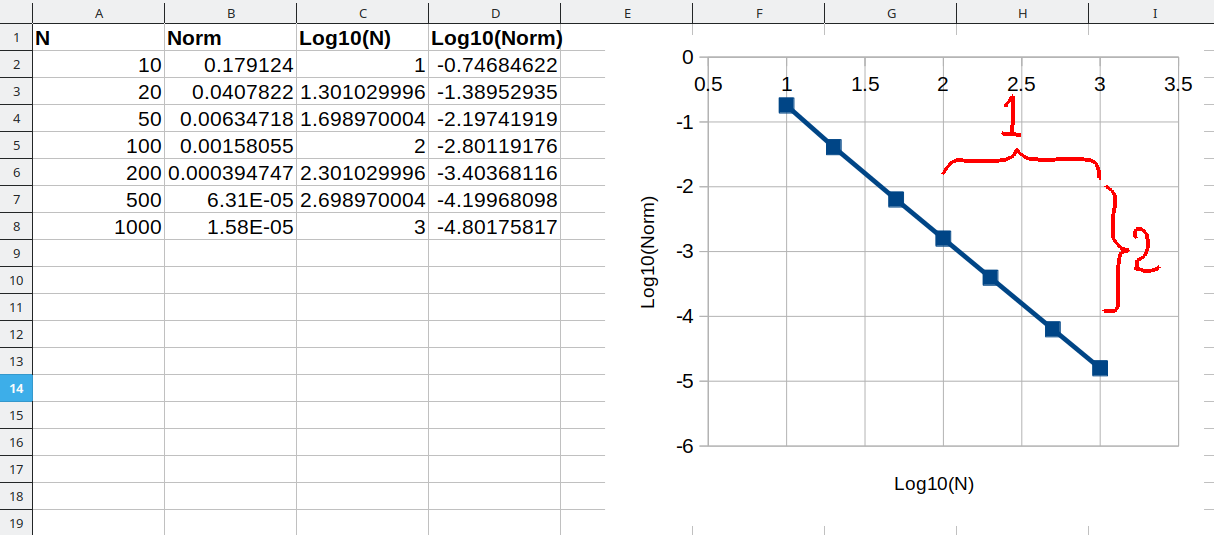
\includegraphics[width=0.9\linewidth]{poisson1_appr.png}
\caption{Сходимость с уменьшением разбиения при решении одномерного уравнения Пуассона}
\label{fig:poisson_convergence}
\end{figure}

Открыв один из cохранённых в процессе работы файлов vtk \ename{poisson1_ncells=?.vtk} в paraview
можно посмотреть полученные графики. В файле представлены как точное ``exact'', так и численное решение ``numerical''
(\figref{fig:poisson_graph}).

\begin{figure}[h]
\centering
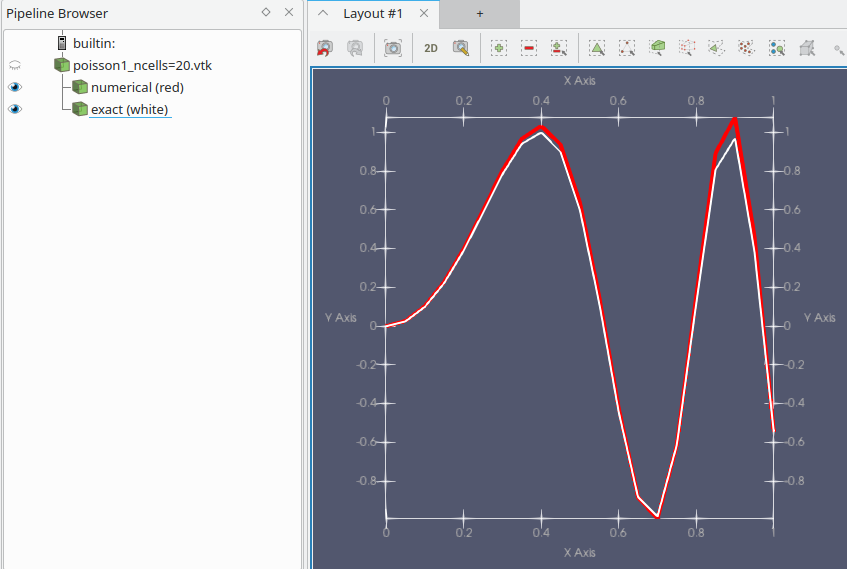
\includegraphics[width=0.9\linewidth]{poisson1_graph.png}
\caption{Сравнение точного и численного решений уравнения Пуассона}
\label{fig:poisson_graph}
\end{figure}


\subsubsubsection{Детали реализации}
\clisting{open}{"test/poisson_fdm_solve_test.cpp"}
Основная работа по решению задачи проводится в классе \cvar{TestPoisson1Worker}.

В его конструкторе происходит инициализация сетки (приватного поля класса) на отрезке $[0, 1]$ с заданным разбиением
\cvar{n_cells}:
\clisting{line}{"TestPoisson1Worker"}

В методе \cvar{solve()} производится чиленное решения задачи и вычисления нормы.
Для этого последовательно
\begin{enumerate}
\item Строится матрица левой части и вектор правой части определяющей системы уравнений.
      Матрицы хранятся в разреженном формате CSR, удобном для последовательного чтения.
\item Вызывается решатель СЛАУ. Решение записывается в приватное поле класса \cvar{u}.
\item Вызывается функция вычисления нормы.
\end{enumerate}

\clisting{block}{"double solve()"}

Функции нижнего уровня (используемые в методе \cvar{solve}):
\begin{itemize}
\item
  Сборка левой части СЛАУ. Реализует формулу \eqref{eq:poisson1d_fdm_lhs}.
  Для заполнения матрицы используется формат \cvar{cfd::LodMatrix}, удобный для непоследовательной записи, который в конце конвертируется CSR.
  \clisting{block}{"approximate_lhs("}
\item
  Сборка правой части СЛАУ. Реализует формулу \eqref{eq:poisson1d_fdm_rhs}.
  \clisting{block}{"approximate_rhs("}
\item
  Вычисление нормы. Реализует формулу \eqref{eq:poisson1d_fdm_norm}.
  \clisting{block}{"compute_norm2"}
\end{itemize}

\clearpage
\subsection{Задание для самостоятельной работы}

\subsubsection{Одномерное уравнение Пуассона}

Скомпиллировать и запустить программу, описанную в п. \ref{sec:poisson1d_prog}.
Построить график полученного численного и точного решения, аналогичный \figref{fig:poisson_graph}
(инструкцию по построению одномерного графика решения в Paraview см. в п \ref{sec:paraview-1d}).

Построить график, подтверждающий второй порядок точности
разностной схемы \eqref{eq:poisson1d_fdm}.

\subsubsection{Двумерное уравнение Пуассона}
\label{sec:hw_poisson_2d}

Написать тест, аналогичный \cvar{[poisson1]}, но
для двумерной задачи на двумерной регулярной сетке
\begin{equation*}
   -\left(\dfrq{u}{x} + \dfrq{u}{y}\right) = f(x, y).
\end{equation*}
использовать разностную схему
\begin{equation*}
   \frac{-u_{k[i-1,j]} + 2 u_{k[i, j]} - u_{k[i+1,j]}}{h_x^2} +
   \frac{-u_{k[i,j-1]} + 2 u_{k[i, j]} - u_{k[i,j+1]}}{h_y^2} =
   f_{k[i,j]},
\end{equation*}
где
\begin{equation}
    \label{eq:tasks_ij2k}
    k[i, j] = i + (n_x+1) j
\end{equation}
-- функция, переводящая парный $(i,j)$ индекс узла регурярной сетки ($i$) для оси x, $j$ для оси y) в сквозной индекс $k$
сеточного вектора, $n_x$ -- количество ячеек сетки в направлении x.

При вычислении весов $w_k$ для вычисления среднеквадратичного отклонения учесть
наличие граничных и угловых точек:
\begin{equation*}
    w_k = \begin{cases}
            h_x h_y / 4,  &\quad  \text{для угловых точек};\\
            h_x h_y / 2,  &\quad  \text{для граничных неугловых точек};\\
            h_x h_y,      &\quad  \text{для внутренних точек}.
    \end{cases}
\end{equation*}
Четрые угловые точки определяются как
\begin{equation*}
    i[k], j[k] = (0, 0), \, (0, n_y), \, (n_x, n_y), \, (n_x, 0)
\end{equation*}
Граничные неугловые точки:
\begin{equation*}
    \begin{array}{lll}
        i[k], j[k] =& \overline{1,n_x-1}, 0;    & \text{нижняя сторона},\\
                    & n_x, \overline{1,n_y-1};  & \text{правая сторона},\\
                    & \overline{1, n_x-1}, n_y; & \text{верхняя сторона},\\
                    & 0, \overline{1,n_y-1};    & \text{левая сторона}.
    \end{array}
\end{equation*}
Функции, переводящие сквозной индекс в пару $i,j$, имеют вид
\begin{equation}
    \label{eq:tasks_k2ij}
    \begin{array}{ll}
        i[k] = {\rm mod}\left(k, \left(n_x+1\right)\right), & \text{// остаток от деления},\\
        j[k] = \lfloor k / \left(n_x+1\right)\rfloor,       &\text{// целая часть от деления}.\\
    \end{array}
\end{equation}

Использовать класс \cvar{cfd::RegularGrid2D} для задания сетки.
Функции перевода индексов узлов из сквозных в парные и обратно реализованы в классе двумерной регулярной сетки:
\begin{itemize}
\item \cvar{cfd::RegularGrid2D::to_split_point_index}
\item \cvar{cfd::RegularGrid2D::to_linear_point_index}
\end{itemize}

В случае, если решатель системы линейных уравнений не решает построенную матрицу, использовать функцию
\cvar{cfd::dbg::print} для отлаточной печати матрицы в консоль (размерность задачи должна быть небольшой).

Для иллюстрации двумерного решения в Paraview использовать изолинии (\ref{sec:paraview-isolines}) и трёхмерные поверхности (\ref{sec:paraview-2d}).

Построить график сходимости для двумерного случая.
Следует иметь ввиду, что на графике сходимости
по оси абсцисс отложено линейное разбиение, вычисляемое как
$n=\sfrac{1}{h}$, где $h$ -- это характерный линейный размер ячейки.
Для двумерных сеток этот линейный размер
сетки можно вычислить через среднюю площадь ячейки $A$ как $h = \sqrt{A}$,
которую в свою очередь можно получить, разделив общую площадь на количество
ячеек: $A = \sfrac{|D|}{N}$. Тогда, в случае единичного квадрата, линейное разбиение будет равно $n = \sqrt{N}$.

\section{Лекция 4 (02.03)}
\subsection{Форматы хранения разреженных матриц}
\subsubsection{CSR-формат}
\label{sec:csr}
При реализации решателей систем сеточных уравнений важно учитывать
разреженный характер используемых в левой части. То есть избегать
хранения и ненужных операций с нулевыми элементами матрицы.

Хотя рассмотренные ранее алогритмы конечноразностных аппроксимаций на структурированных сетках
давали трёх- (для одномерных задач) или пятидиагональную (для двумерных) сеточную матрицу,
здесь будем рассматривать общие форматы хранения, не привязанные к конкретному шаблону.

Любой общий
формат хранения должен хранить
информацию о шаблоне матрице (адресах ненулевых элементов)
и значениях матричных коэффициентов в этом шаблоне.

В CSR (Compressed sparse rows) формате
все ненулевые элементы хранятся в линейном массиве \ename{vals}.
А шаблон матрицы -- в двух массивах
\begin{itemize}
	\item массиве колонок \ename{cols} -- значений колонок для соответствующих ему значений из массива \ename{vals},
	\item массиве адресов \ename{addr} -- индексах массива \ename{vals}, с которых начинается описание соответствующей строки.
\end{itemize}
В конце массива \ename{addr} добавляется общая длина массива \ename{vals}.

Таким образом, длины массивов \ename{vals}, \ename{cols} равны количеству ненулевых элементов матрицы,
а длина массива \ename{addr} равна количеству строк в матрице плюс один.

Для облегчения процедур поиска описание каждой строки должно идти последовательно
с увеличением индекса колонки.

Для примера рассмотрим следующую матрицу
\begin{equation}
\label{eq:example-sparse-matrix}
\left(
\begin{array}{cccc}
2.0 & 0 & 0 & 1.0 \\
0 & 3.0 & 5.0 & 4.0 \\
0 & 0 & 6.0 & 0 \\
0 & 7.0 & 0 & 8.0 \\
\end{array}
\right)
\end{equation}

Массивы, описывающие матрицу в формате CSR примут вид

\begin{equation*}
\begin{array}{r|l|l|l|l|l}
      & row=0     & row=1          & row=2& row=3&\\
\hline
vals= & 2.0, 1.0, & 3.0, 5.0, 4.0, & 6.0, & 7.0, 8.0 &\\
\hline
cols= & 0,\phantom{.0} 3,\phantom{.0}      & 1,\phantom{.0}2,\phantom{.0}3,\phantom{.0}          & 2,\phantom{.0}   & 1,\phantom{.0} 3     &\\
\hline
addr= & 0,        & 2,             & 5,   & 6,       & 8 \\
\hline
\end{array}
\end{equation*}

Рассмотрим реализацию базовых алгоритмов для матриц, заданных в этом формате.

Пусть матрица задана следующими массивами:
\begin{minted}[linenos=false]{c++}
std::vector<double> vals; // массив значений
std::vector<size_t> cols; // массив столбцов
std::vector<size_t> addr; // массив адресов
\end{minted}

Число строк в матрице:
\begin{minted}[linenos=false]{c++}
size_t nrows = addr.size()-1;
\end{minted}

Число элементов в шаблоне (ненулевых элементов)
\begin{minted}[linenos=false]{c++}
size_t n_nonzeros = vals.size();
\end{minted}

Число ненулевых элементов в заданной строке `irow`
\begin{minted}[linenos=false]{c++}
size_t n_nonzeros_in_row = addr[irow+1] - addr[irow];
\end{minted}

Умножение матрицы на вектор `v` (длина этого вектора должна быть равна числу строк в матрице).
Здесь реализуется суммирование вида
\begin{equation*}
    r_i = \sum_{j=0}^{N-1} A_{ij} v_j,
\end{equation*}
при этом избегаются лишние операции с нулями
\begin{minted}[linenos=false]{c++}
// число строк в матрице и длина вектора v
size_t nrows = addr.size() - 1;
// массив ответов. Инициализируем нулями
std::vector<double> r(nrows, 0);
// цикл по строкам
for (size_t irow=0; irow < nrows; ++irow){
	// цикл по ненулевым элементам строки irow
	for (size_t a = addr[irow]; a < addr[irow+1]; ++a){
		// получаем индекс колонки
		size_t icol = cols[a];
		// значение матрицы на позиции [irow, icol]
		double val = vals[a];
		// добавляем к ответу
		r[irow] += val * v[icol];
	}
}
\end{minted}


Поиск значения элемента матрицы по адресу \cvar{(irow, icol)} с учётом локально сортированного вектора \cvar{cols}
\begin{minted}[linenos=false]{c++}
using iter_t = std::vector<size_t>::const_iterator;
// указатели на начало и конец описания строки в массиве cols
iter_t it_start = cols.begin() + addr[irow];
iter_t it_end = cols.begin() + addr[irow+1];
// поиск значения icol в отсортированной последовательности [it_start, it_end)
iter_t fnd = std::lower_bound(it_start, it_end, icol);
if (fnd != it_end && *fnd == icol){
	// если нашли, то определяем индекс найденного элемента в массиве cols
	size_t a = fnd - cols.begin();
	// и возвращаем значение из vals по этому индексу
	return vals[a];
} else {
	// если не нашли, значит элемент [irow, icol] находится вне шаблона. Возвращаем 0
	return 0;
}
\end{minted}

Формат CSR обеспечивает максимальную компактность хранения
разреженной матрицы и при этом удобен для последовательной итерации по элементам матрицы (операции умножения матрицы на вектор),
но его существенным недостатком является высокая сложность добавления нового элемента в шаблон.

\subsubsection{Массив словарей}
При реализации сеточных методов решения дифференциальных уравнений работу с матрицами
можно разбить на два этапа: сборка матриц и их непосредственное использование.
Сборка матрицы в свою очередь может быть разделена на
этап вычисление шаблона матрицы (символьная сборка) и
непосредственное вычисление коэффициентов матрицы (числовая сборка).

На этапе использования матрицы основной операцией
является умножение матрицы на вектор, где наиболее эффективным является CSR-формат.

В случае использования неструктурированных сеток этап символьной сборки
является нетривиальной операцией и сводится к неупорядоченному добавлению
новых элементов в шаблон матрицы. Как было отмечено ранее, 
такая операция в случае использования CSR формата неэффективена.

Поэтому часто для этапов сборки и расчёта используют
разные форматы хранения матриц, первый из которых оптимизирован для операции вставки, а второй -- для операции умножения на вектор.
В качестве формата, оптимизированного для вставки, можно представить формат массива словарей (List of dictionaries), где каждая строка матрицы
описывается словарём, ключём которого является индекс колонки, а значением -- величина соответствующего матричного коэффициента.

С использованием синтаксиса C++ такой формат может быть описан следующим образом:
\begin{cppcode}
std::vector<std::map<size_t, double>> data;
\end{cppcode}

Марица вида \eqref{eq:example-sparse-matrix} в таком формате примет вид
\begin{cppcode}
data = {
	{0: 2.0, 3: 1.0},
	{1: 3.0, 2: 5.0, 3: 4.0},
	{2: 6.0},
	{1: 7.0, 3: 8.0}
};
\end{cppcode}

Добавление нового матричного коэффициента сведётся к вставке элемента в словарь:
\begin{cppcode}
data[i][j] = value;
\end{cppcode}

А основной операцией для такого формата будет служить
конверсия в CSR:
\begin{cppcode}
std::vector<size_t> addr{0};
std::vector<size_t> cols;
std::vector<double> vals;
for (size_t irow=0; irow < data.size(); ++irow){
	for (auto it: data[irow]){
		cols.push_back(it.first);
		vals.push_back(it.second);
	}
	addr.push_back(addr.back() + data[irow].size());
}
\end{cppcode}
Поскольку данные в контейнере типа \cvar{std::map} итерируются
в отсортированном по ключам порядке, то полученный
в результе массив \cvar{cols} также является локально отсортированным.

\section{Лекция 5 (09.03)}
\subsection{Решение СЛАУ}

В рассмотренных ранее примерах использовался алгебраический
многосеточный итерационный решатель, который имеет существенное время
инициализации. Ниже рассмотрим некоторые более простые итерационные способы решения систем
уравнений, которые, хотя и имеют значительно худшую сходимость, но не требуют дорогой инициализации.

\subsubsection{Метод Якоби}
\label{sec:SLAE-Jacobi}

Будем рассматривать систему уравнений вида
\begin{equation*}
    \sum_{j=0}^{N-1} A_{ij} u_j = r_i, \quad i = \overline{0, N-1}
\end{equation*}
относительно неизвестного сеточного вектора $\{u\}$.

В классическом виде алгоритм Якоби формулируется в виде
\begin{equation*}
    \hat u_i = \frac{1}{A_{ii}}\left(r_i - \sum_{j\neq i} A_{ij}{u_j}\right)
\end{equation*}

Произведём некоторые преобразования
\begin{align*}
    \hat u_i &= \frac{1}{A_{ii}}\left(r_i - \sum_{j} A_{ij}{u_j} + A_{ii}u_i\right) \\
             &= u_i + \frac{1}{A_{ii}}\left(r_i - \sum_{j} A_{ij}{u_j}\right)
\end{align*}

Таким образом, программировать итерацию этого алгоритма, обновляющую значения массива $\{u\}$, можно в виде
\begin{align*}
    &\check u = u; \\
    &\textbf{for } i=\overline{0, N-1} \\ 
    &\quad u_i \mathrel{{+}{=}} \frac{1}{A_{ii}}\left(r_i - \sum_{j=0}^{N-1} A_{ij}{\check u_j}\right)\\
    &\textbf{endfor} \\
\end{align*}


\subsubsection{Метод Зейделя}
\label{sec:SLAE-Seidel}
Формулируется в виде
\begin{equation*}
    \hat u_i = \frac{1}{A_{ii}}\left(r_i - \sum_{j<i} A_{ij}{\hat u_j} - \sum_{j>i} A_{ij}{u_j} \right).
\end{equation*}

Поскольку этот метод неявный относительно уже найденных на итерации значений, то в отличии от метода Якоби этот алгоритм не требует создания временного массива $\hat u$
при программировании. Псевдокод для реализации итерации этого метода можно записать как

\begin{align*}
    &\textbf{for } i=\overline{0, N-1} \\ 
    &\quad u_i \mathrel{{+}{=}} \frac{1}{A_{ii}}\left(r_i - \sum_{j=0}^{N-1} A_{ij}{u_j}\right)\\
    &\textbf{endfor}
\end{align*}


\subsubsection{Метод последовательных верхних релаксаций (SOR)}
\label{sec:SLAE-SOR}
Этот метод основан на добавлении к решению результатов итераций Зейделя с
коэффициентом $\omega > 1$. То есть он изменияет решение по тому же
принципу, что и метод Зейделя, но искуственно увеличивает эту добавку.

Формулируется этот метод в виде
\begin{equation*}
    \hat u_i = (1-\omega) u_i + \frac{\omega}{A_{ii}}\left(r_i - \sum_{j<i} A_{ij}{\hat u_j} - \sum_{j>i} A_{ij}{u_j} \right).
\end{equation*}
Для устойчивости метода необходимо $\omega < 2$. В частности, для одномерных задач,
заданных на единичном отрезке, для оптимальной сходимости можно использовать соотношение $\omega \approx 2 - 5 h$,
где $h$ -- шаг сетки.

Итерация этого метода по аналогии с методом Зейделя может быть запрограммирована в виде

\begin{align*}
    &\textbf{for } i=\overline{0, N-1} \\ 
    &\quad u_i \mathrel{{+}{=}} \frac{\omega}{A_{ii}}\left(r_i - \sum_{j=0}^{N-1} A_{ij}{u_j}\right)\\
    &\textbf{endfor}
\end{align*}

\subsection{Задание для самостоятельной работы}

Вернутся к рассмотрению двумерного уравнения Пуассона (п.~\ref{sec:hw_poisson_2d}).
Прошлая реализация этой задачи
включала в себя решение СЛАУ алгебраическим многосеточным методом
с помощью класса \cvar{AmgcMatrixSolver}:
\begin{cppcode}
	AmgcMatrixSolver solver;
	solver.set_matrix(mat);
	solver.solve(rhs, u);
\end{cppcode}

Необходимо реализовать рассмотренные ранее методы
итерационного решения СЛАУ

\begin{itemize}
\item метод Якоби (\ref{sec:SLAE-Jacobi}),
\item метод Зейделя (\ref{sec:SLAE-Seidel}),
\item метод SOR (\ref{sec:SLAE-SOR}).
\end{itemize}
и использовать их вместо многосеточного решателя.

Реализовать означенные решатели нужно в виде функций вида:
\begin{cppcode}
// Single Jacobi iteration for mat*u = rhs SLAE. Writes result into u
void jacobi_step(const cfd::CsrMatrix& mat, const std::vector<double>& rhs, std::vector<double>& u){
    ...
}
\end{cppcode}
которые делают одну итерацию соответствующего метода без проверок на сходимость.
Аргумент \cvar{u} используется как начальное значение искомого сеточного вектора. Туда же пишется 
итоговый результат.

Все алгоритмы основаны на вычислении выражения вида
\begin{equation*}
   \frac{1}{A_{ii}}\left(r_i - \sum_{j=0}^{N-1} A_{ij}{u_j}\right),
\end{equation*}
поэтому рекомендуется выделить отдельную функцию, которая бы вычисляла это выражение
и использовалась всеми тремя решателями
\begin{minted}[linenos=false]{c++}
double row_diff(size_t irow, const cfd::CsrMatrix& mat, const std::vector<double>& rhs, const std::vector<double>& u){
	const std::vector<size_t>& addr = mat.addr();   // массив адресов
	const std::vector<size_t>& cols = mat.cols();   // массив колонок
	const std::vector<double>& vals = mat.vals();   // массив значений
    ...
}
\end{minted}

Дополнительно понадобится реализовать функцию, которая проверяет сходимость решения
путём вычисления невязки вида
\begin{equation*}
res = \max_i{\left| \sum_{j}A_{ij} u_j - r_i \right|}
\end{equation*}
и сравнения с заданным малым числом $\eps=10^{-8}$.
\begin{cppcode}
bool is_converged(const cfd::CsrMatrix& mat, const std::vector<double>& rhs, const std::vector<double>& x){
	constexpr double EPS = 1e-8;
	double residual = 0;
	// ...
	return residual < EPS;
}
\end{cppcode}

Для реализации вспомогательных функций необходимо
использоватть алгоритмы работы с CSR-матрицами из п.~\ref{sec:csr}

При реализации метода SOR подобрать оптимальный параметр $\omega$,
при котором метод SOR сойдётся за минимальное число итераций.

После реализации всех методов необходимо
сравнить время исполнения решателей. Замеры нужно проводить в Release-версии сборки (см. п.~\ref{sec:release-build}).
Для замера времени исполнения участка кода воспользоваться функциями
\begin{itemize}
\item \cvar{cfd::dbg::Tic} -- вызвать до начала участка кода
\item \cvar{cfd::dbg::Toc} -- вызвать после окончания участка кода
\end{itemize}

Код решения СЛАУ методом Якоби с вызовами профилироващика
должен иметь примерно такой вид:
\begin{cppcode}
#include "dbg/tictoc.hpp"
using namespace cfd;

...

// реализация решения СЛАУ
dbg::Tic("total");  // запустить таймер total
for (size_t it=0; it < max_it; ++it){
	dbg::Tic("step");  // запустить таймер step
	jacobi_step(mat, rhs, u);
	dbg::Toc("step");  // остановить таймер step

	dbg::Tic("conv-check");  // запустить таймер conv-check
	bool is_conv = is_converged(mat, rhs, u);
	dbg::Toc("conv-check");  // остановить таймер conv-check

	if (is_conv) break;
}
dbg::Toc("total");  // остановить таймер total
\end{cppcode}

При правильном задании функций замеров, по окончанию работы в консоль должен напечататься отчёт о времени исполнения вида:
\begin{shelloutput}
     total:  6.670 sec
      step:  5.220 sec
conv-check:  1.210 sec
\end{shelloutput}

По результатам профилировки нужно заполнить таблицу

\begin{equation*}
\begin{array}{l|c|c|c|c|c|c}
    Метод & \text{total, s} & \text{step, s} & \text{conv-check, s} & \text{Кол-во итераций} \\
    \hline
    \text{Amg} &   & - & - & - \\
    \hline
    \text{Якоби} &   &  &  & \\
    \hline
    \text{Зейдель} &   &  &  & \\
    \hline
    \text{SOR} (\omega=...)&   &   & & \\
\end{array}
\end{equation*}
Здесь Amg - исходный решатель.

\section{Лекция 6 (23.03)}

\subsection{Метод конечных объёмов}
\subsubsection{Уравнение Пуассона}
Пространственную аппроксимацию дифференицальных операторов
методом конечных объёмов рассмотрим на примере многомерного уравнения Пуассона
\begin{equation}
\label{eq:fvm_pois}
-\nabla^2 u = f,
\end{equation}
которое требуется решить в области $D$. Разобъём эту область
на непересекающиеся подобласти $E_i$, $i = \overline{0, N-1}$ (\figref{fig:fvm_grid}).
Центры ячеек обозначим как $\vec c_i$.

\begin{figure}[h!]
\centering
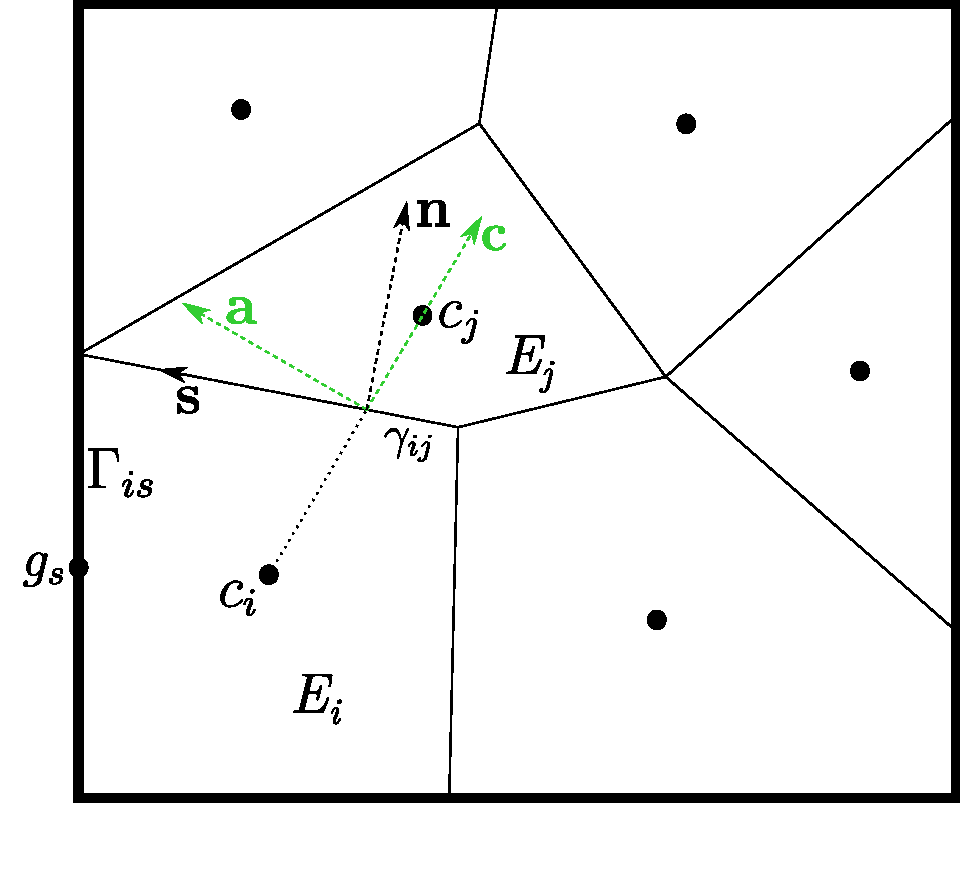
\includegraphics[width=0.4\linewidth]{fvm_grid.pdf}
\caption{Конечнообъёмная сетка}
\label{fig:fvm_grid}
\end{figure}

Проинтегрируем исходное уравнение
по одной из подобластей $E_i$:
\begin{equation*}
-\arint{\nabla^2 u}{E_i}{s} = \arint{f}{E_i}{\vec x}.
\end{equation*}
К интегралу в левой части применим формулу интегрирования по частям \cref{eq:partint_laplace}. Получим
\begin{equation}
\label{eq:fvm_pois_int}
-\arint{\dfr{u}{n}}{\partial E_i}{s} = \arint{f}{E_i}{\vec x}.
\end{equation}
Здесь $\partial E_i$ -- совокупность всех границ подобласти $E_i$,
а $\vec n$ -- внешняя к подобласти нормаль.

Граница ячейки $E_i$ состоит из внутренних граней $\gamma_{ij}$ (индекс $j$ здесь
соответствует индексу соседней ячейки)
и граней $\Gamma_{is}$, лежащих на внешней границе расчётной области $D$.
Тогда интеграл по общей границе ячейки распишется через сумму интегралов по плоским поверхностям
$$
\arint{\dfr{u}{n}}{\partial E_i}{s} = \sum_j\arint{\dfr{u}{n}}{\gamma_{ij}}{s} + \sum_s\arint{\dfr{u}{n}}{\Gamma_{is}}{s}.
$$
Аппроксимирум производную $\dsfr{u}{n}$ на каждой из граней константой.
Тогда её можно вынести из под интегралов и предыдущее выражение записать в виде
\begin{equation}
\label{eq:fvm_gamma_integral}
\arint{\dfr{u}{n}}{\partial E_i}{s} \approx
\sum_j
    \left|
        \gamma_{ij}
    \right|
    \left(
        \dfr{u}{n}
    \right)_{\gamma_{ij}}
+\sum_s
    \left|
        \Gamma_{is}
    \right|
    \left(
        \dfr{u}{n}
    \right)_{\Gamma_{is}}
\end{equation}

Аналогично, анализируя интеграл правой части \cref{eq:fvm_pois_int},
приблизим значение функции правой части $f$ внутри элемента $E_i$ константой $f_i$,
которую отнесём к центру элемента. Тогда
\begin{equation}
\label{eq:fvm_f_integral}
\arint{f}{E_i}{\vec x} \approx f_i \left|E_i\right|.
\end{equation}

Сеточный вектор $\{f_i\}$ -- есть конечнообъёмная аппроксимация
функции $f(\vec x)$ на конечнообъёмную сетку.
Значения $f_i$ при аппроксимации чаще всего находятся как значения в центрах элементов
$$
f_i = f(\vec c_i).
$$
Хотя иногда может быть использовано и другое определение,
следующее из \eqref{eq:fvm_f_integral}:
$$
f_i = \frac{1}{\left| E_i \right|} \arint{f(\vec x)}{E_i}{\vec x}.
$$


\subsubsubsection{Обработка внутренних граней}
Для начала будем рассматривать сетки, в
которых вектора $\vec c$, соединяющие центры ячеек (зедёные вектора на \figref{fig:fvm_grid}),
коллинеарны (или почти коллинеарны) нормалям к граням $\vec n$.
В этом случае производную искомой функции по нормали к грани можно записать в виде
$$
\dfr{u}{n} = \dfr{u}{c}.
$$

Далее определим значения функции $u$ в точках $c_i$, $c_j$ как $u_i$, $u_j$.
Тогда значение производной $\dsfr{u}{n}$ на внутренней грани конечного объёма
может быть приближена конечной разностью
\begin{equation}
\label{eq:fvm_dudn_dudc}
\dfr{u}{n} = \dfr{u}{c} \approx \frac{u_j - u_i}{h_{ij}}, \quad h_{ij} = |\vec c_j - \vec c_i|.
\end{equation}

Определим pebi (perpendicular-bisector) сетки как сетки, удовлетворяющие следующим свойствам
\begin{itemize}
\item линии, соединяющие центры двух соседних ячеек, перпендикулярны грани между этими ячейками;
\item внутренние грани делят линии, соединящие центры соседних ячеек, пополам.
\end{itemize}
Очевидно, что равномерная структурированная сетка удовлетворяет этим свойствам.
Для построения неструктурированных pebi-сеток используют алгоритмы построения ячеек Вороного.
Для pebi-сеток разностная схема \eqref{eq:fvm_dudn_dudc}
является симметричной разностью и, поэтому, имеет второй порядок аппроксимации.

\subsubsubsection{Учёт граничных условий первого рода}
Для вычисления второго слагаемого в правой части 
\cref{eq:fvm_gamma_integral}
следует расписать значение нормальной 
к границе производной вида
$$
\left(\dfr{u}{n}\right)_{\Gamma_{is}}.
$$
Это делается с помощью граничных условий.

Пусть на центре грани $\Gamma_{is}$ задано 
значение искомой функции
\begin{equation}
\label{eq:fvm_bc1}
\vec x \in \Gamma_{is}: \quad u(\vec x) = u^\Gamma.
\end{equation}
Аппроксимацию производных
будем проводить из тех же соображений, которые использовали
при анализе внутренних граней. Только вместо центра соседнего элемента
$c_j$ будем использовать центр грани $g_s$.
В первом приближении, отбрасывая касательные производные, придём к формуле аналогичной \cref{eq:fvm_dudn_dudc}:
\begin{equation}
\label{eq:fvm_bc1_approx}
\dfr{u}{n} \approx \frac{u^\Gamma - u_i}{h_{is}}, \quad h_{is} = \left| \vec g_s  - \vec c_i \right|.
\end{equation}

\subsubsection{Одномерный случай}
Рассмотрим результат конечнообъёмной аппроксимации
задачи \cref{eq:fvm_pois} в одномерном случае
на равномерной сетке с шагом $h$ (\figref{fig:fvm_grid1d}).

\begin{figure}[h!]
\centering
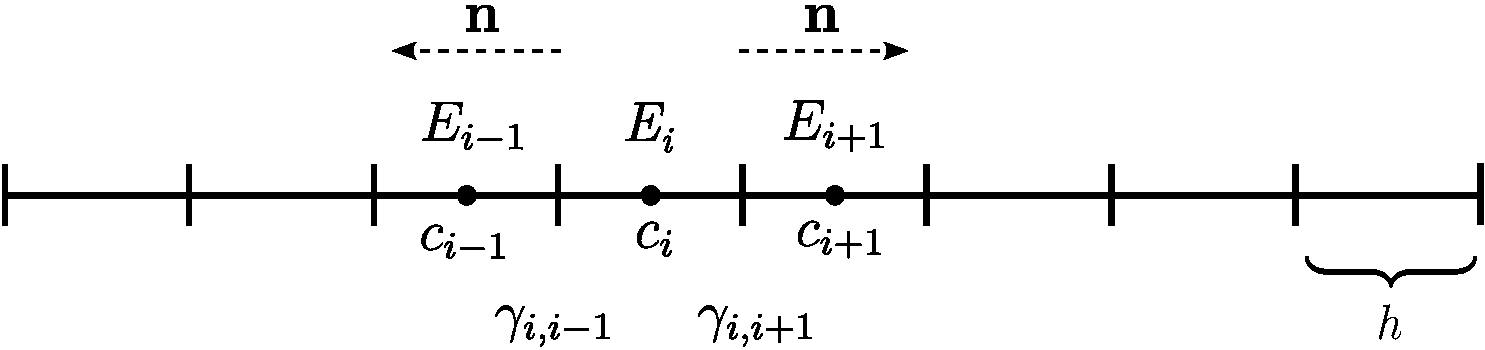
\includegraphics[width=0.6\linewidth]{fvm_grid1d.pdf}
\caption{Одномерная конечнообъёмная сетка}
\label{fig:fvm_grid1d}
\end{figure}

У внутренней ячейки $i$ есть две границы: $\gamma_{i,i-1}$ и $\gamma_{i,i+1}$.
Нормали по этим границам аппроксимируются по формулам \cref{eq:fvm_dudn_approx}:
\begin{align*}
\gamma_{i,i-1}: \quad& \dfr{u}{n} = \frac{u_{i-1}-u_{i}}{h} \\[10pt]
\gamma_{i,i+1}: \quad& \dfr{u}{n} = \frac{u_{i+1}-u_{i}}{h}
\end{align*}
Объём ячейки в одномерном случае равен её длине $h$.
Площадь грани следует положить единице с тем, чтобы
$$
|E_i| = |\gamma| h = h.
$$
Тогда, подставляя эти значения в \cref{eq:fvm_pois_int},
получим знакомую конечноразностную схему аппроксимацию уравнения Пуассона
$$
\frac{-u_{i-1} + 2 u_i - u_{i+1}}{h} = f_i h,
$$
которая имеет второй порядок точности.
Разница с методом конечных разностей здесь состоит в том,
что значения сеточных векторов $\gvec{u}$, $\gvec{f}$ здесь
приписаны к центрам ячеек, а не к их узлам.
Это отличие проявит себя в аппроксимации граничных условий.
Так, если на левой границе задано условие первого рода, то соответствующее уравнение
согласно \cref{eq:fvm_bc1_approx}
примет вид
$$
-\frac{u^\Gamma - u_0}{h/2} - \frac{u_1 - u_0}{h} = f_0 h.
$$
В методе конечных разностей это условие выразилось бы в виде $u_0 = u^\Gamma$.

\subsubsection{Сборка системы линейных уравнений}
Подставим все полученные аппроксимации
\cref{eq:fvm_dudn_dudc,eq:fvm_bc1_approx}
в уравнение \cref{eq:fvm_pois_int}:
\begin{equation*}
-\sum_j
    \frac{|\gamma_{ij}|}{h_{ij}}
         \left(u_j - u_i\right)
-\sum_{s\in{\rm I}}
    \frac{|\Gamma_{is}|}{h_{is}}
        \left(u^\Gamma - u_i\right)
=
f_i |E_i|.
\end{equation*}
Здесь первое слагаемое в левой части отвечает за потоки через внутренние границы,
второе -- граничные условия первого рода.
Далее перенесём все известные значения в правую часть и окончательно
получим линейное уравнение для $i$-го конечного объёма:
\begin{equation}
\label{eq:fvm_slae}
\sum_j
    \frac{|\gamma_{ij}|}{h_{ij}}
         \left(u_i - u_j\right)
+\sum_{s\in{\rm I}}
    \frac{|\Gamma_{is}|}{h_{is}}u_i
 =
f_i |E_i|
+\sum_{s\in{\rm I}}
    \frac{|\Gamma_{is}|}{h_{is}} u^\Gamma
\end{equation}
Таким образом мы получили систему из $N$ (по количеству подобластей) линейных уравнений относительно
неизвестного сеточного вектора $\left\{u_i\right\}$
$$
A u = b.
$$

\subsubsubsection{Алгоритм сборки в цикле по ячейкам}
Матрицу $A$ и правую часть $b$ системы \cref{eq:fvm_slae} можно
собирать в цикле по ячейкам: строчка за строчкой.
Такой алгоритм выглядел бы следующим образом
\begin{equation*}
\begin{array}{ll}
\textbf{for } i = \overline{0, N-1}                          & \textrm{-- цикл по строкам СЛАУ}\\
\qquad b_i = |E_i| f_i                                       & \\
\qquad \textbf{for } j \in \textrm{nei(i)}                   & \textrm{-- цикл по ячейкам, соседним с ячейкой $i$}\\
\qquad \qquad v = \sfrac{|\gamma_{ij}|}{h_{ij}}              & \\
\qquad \qquad A_{ii} \pluseq v                               & \\
\qquad \qquad A_{ij} \minuseq v                              & \\
\qquad \textbf{endfor}                                       & \\
\qquad \textbf{for } s \in \textrm{bnd1(i)}                  & \textrm{-- цикл по граням ячейки $i$ с условиями первого рода}\\
\qquad \qquad v = \sfrac{|\Gamma_{is}|}{h_{is}}              & \\
\qquad \qquad A_{ii} \pluseq v                               & \\
\qquad \qquad b_{i}  \pluseq u^{\Gamma} v                    & \\
\qquad \textbf{endfor}                                       & \\
\textbf{endfor}
\end{array}
\end{equation*}
Первым недостатком такого алгоритма является наличие вложенных циклов.
Во-вторых, коэффициент, отвечающий за поток через внутреннюю грань $\gamma_{ij}$,
равный $\sfrac{|\gamma_{ij}|}{h_{ij}}$ в таком алгоритме будет учитываться дважды:
в строке $i$ и в строке $j$.

\subsubsubsection{Алгоритм сборки в цикле по граням}
Вместо общего цикла по ячейкам, будем использовать цикл по граням.
В таком цикле коэффициенты потоков будут вычисляться один раз
и вставляться сразу в две строки матрицы, соответствующие соседним с гранью ячейкам.
Вложенных циклов в такой постановке удаётся избежать, потому
что у грани есть только две соседние ячейки (в то время как у ячейки может быть произвольное
количество соседних граней).

Разделим все грани на исходной сетки на внутренние и граничные (отдельный набор для каждого вида граничных условий).
Тогда для внутренних граней можно записать
\begin{equation}
\label{eq:fvm_assem_internal}
\begin{array}{ll}
\textbf{for } s \in\textrm{internal}                     & \textrm{-- цикл по внутренним граням}\\ 
\qquad i,j = \textrm{nei\_cells(s)}                      & \textrm{-- две ячейки, соседние с текущей гранью}\\
\qquad v = \sfrac{|\gamma_{ij}|}{h_{ij}}                 & \\
\qquad A_{ii} \pluseq  v; \quad A_{jj} \pluseq  v        & \textrm{-- диагональные коэффициенты матрицы}\\ 
\qquad A_{ij} \minuseq v; \quad A_{ji} \minuseq v        & \textrm{-- внедиагональные коэффициенты матрицы}\\
\textbf{endfor}                                          & \\
\end{array}
\end{equation}
Граничные условия учитываются в отдельных циклах.
Здесь будем учитывать, что у грани, принадлежащей
границе области, есть только одна соседняя ячейка.
Условия первого рода:
\begin{equation}
\label{eq:fvm_assem_bc1}
\begin{array}{ll}
\textbf{for } s \in\textrm{bnd1}                         & \textrm{-- грани с условиями первого рода}\\ 
\qquad i = \textrm{nei\_cells(s)}                        & \textrm{-- соседняя с граничной гранью ячейка}\\
\qquad v = \sfrac{|\Gamma_{is}|}{h_{is}}                 & \\
\qquad A_{ii} \pluseq  v                                 & \\ 
\qquad b_{i} \pluseq u^\Gamma v                          & \\
\textbf{endfor}                                          & \\
\end{array}
\end{equation}
Первое слагаемое в правой части
\cref{eq:fvm_slae}
учтём отдельным циклом:
\begin{equation}
\label{eq:fvm_assem_f}
\begin{array}{ll}                                         & \\
\textbf{for } i = \overline{0,N-1}                        & \textrm{-- цикл по ячейкам}\\ 
\qquad b_i = |E_i| f_i                                    & \\
\textbf{endfor}                                           &
\end{array}
\end{equation}

\subsection{Задание для самостоятельной работы}
\label{sec:hw_fvm2d}
В тесте \cvar{poisson1-fvm} из файла \ename{poisson_fvm_solve_test.cpp}
реализовано решение одномерного уравнения Пуассона с граничными условиями первого рода.
Проводится расчёт на сгущающихся сетках с количеством ячеек от 10 до 1000
и расчитываются среднеквадратичные нормы отклонения полученного численного решения от точного.
Решения сохраняются в vtk-файлы \ename{poisson1_fvm_n={}.vtk}.



Отталкиваясь от этой реализации необходимо:
\begin{enumerate}
\item написать аналогичный тест для двумерного уравнения и случая неструктурированных сеток,
\item провести серию расчётов на сгущающихся сетках разных типов (структурированных, pebi и скошенных)
\item визуализировать решение, полученное на этих сетках
\item построить графики сходимости решения и определить порядок аппроксимации метода
\end{enumerate}

\paragraph{Построение неструктурированных сеток}
В папке \ename{test_data} корневой директории репозитория
лежат скрипты построения сеток в программе \ename{HybMesh}:
\begin{itemize}
\item \ename{pebigrid.py} -- pebi--сетка,
\item \ename{tetragrid.py} -- сетка, состоящая из произвольных (скошенных) трех- и четырехугольников.
\end{itemize}
Инструкции по запуску этих скриптов смотри п. \ref{sec:hybmesh}.
Эти скрипты строят равномерную неструктурированную сетку
в единичном квадрате
и записывают её в файл vtk, который впоследствии можно загрузить
в расчётную программу.
В каждом из скриптов есть параметр \cvar{N}, означающий
примерное количество ячеек в итоговой сетке.
Меняя его значение можно строить сетки разного разрешения.

Для загрузки построенной сетки в решатель необходимо файл
с сеткой поместить в каталог \ename{test_data}
и далее загрузить её в класс \cvar{UnstructuredGrid2D}.
Нижеследующий код прочитает файл \ename{test_data/pebigrid.vtk}
и создаст рабочий класс с использованием прочитанной сетки
\begin{cppcode}
std::string fn = test_directory_file("pebigrid.vtk");
UnstructuredGrid2D grid = UnstructuredGrid2D::vtk_read(fn);
\end{cppcode}

\paragraph{Рекомендации к программированию}
При написании новых тестов следует переиспользовать уже написанный код, избегая копирования.
Для этого необходимо пользоваться механизмами наследования классов.
В частности, следует обратить внимание, что все сетки наследуются
от единого интерфейса \cvar{IGrid}. А уже написанный ``одномерный'' код 
в своей алгоритмической части использует только функции этого интерфейса.

\section{Лекция 7 (30.03)}

\subsection{Граничные условия второго рода}
Учёт условий второго рода тривиален.
Если на центре грани $\Gamma_{is}$ задано 
значение нормальной производной
\begin{equation}
\label{eq:fvm_bc2_approx}
\vec x \in \Gamma_{is}: \quad \dfr{u}{n} = q(\vec x),
\end{equation}
то это значение просто подставляется вместо соответствующей производной
в  \cref{eq:fvm_gamma_integral}.

По аналогии с \eqref{eq:fvm_assem_bc1}
учёт граничных условий второго рода
при сборке по граням будет иметь следующий вид
\begin{equation}
\label{eq:fvm_assem_bc2}
\begin{array}{ll}
\textbf{for } s \in\textrm{bnd2}                         & \textrm{-- грани с условиями второго рода}\\ 
\qquad i = \textrm{nei\_cells(s)}                        & \textrm{-- соседняя с граничной гранью ячейка}\\
\qquad b_{i} \pluseq |\Gamma_{is}| q                     & \\
\textbf{endfor}                                          & \\
\end{array}
\end{equation}


\subsection{Граничные условия третьего рода}
Теперь рассмотрим условия третьего рода
\begin{equation}
\label{eq:fvm_bc3}
\vec x \in \Gamma_{is}: \quad \dfr{u}{n} = \alpha(\vec x) u + \beta(\vec x).
\end{equation}
Распишем производную в форме \cref{eq:fvm_bc1_approx}:
\begin{equation*}
\frac{u^\Gamma - u_i}{h_{is}} = \alpha u^\Gamma + \beta,
\end{equation*}
откуда выразим $u^\Gamma$:
$$
u^\Gamma =  \frac{u_i + \beta h_{is}}{1 - \alpha h_{is}}.
$$
Подставляя это выражение в исходное граничное условие \eqref{eq:fvm_bc3} получим
\begin{equation}
\label{eq:fvm_bc3_approx}
\dfr{u}{n} = \frac{\alpha}{1 - \alpha h_{is}} u_i + \frac{\beta}{1 - \alpha h_{is}}.
\end{equation}

Учёт граничных условий третьего рода при сборке по граням будет иметь вид

\begin{equation}
\label{eq:fvm_assem_bc3}
\begin{array}{ll}
\textbf{for } s \in\textrm{bnd3}                         & \textrm{-- грани с условиями третьего рода}\\ 
\qquad i = \textrm{nei\_cells(s)}                        & \textrm{-- соседняя с граничной гранью ячейка}\\
\qquad v = \sfrac{|\Gamma_{is}|}{(1 + \alpha h_{is})}    & \\
\qquad A_{ii} \minuseq  \alpha v                         & \\ 
\qquad b_{i} \pluseq \beta v                             & \\
\textbf{endfor}                                          &
\end{array}
\end{equation}

\subsubsection{Универсальность условий третьего рода}
Условие третьего рода
\eqref{eq:fvm_bc3}
можно использовать для моделирования условий первого и второго рода.
Так, условия второго рода \cref{eq:fvm_bc2_approx} получаются, если положить $\alpha = 0$, $\beta = q$.
А условия первого \cref{eq:fvm_bc1}, -- если
\begin{equation}
\label{eq:fvm_bc3_universal}
\alpha = \eps^{-1}, \quad \beta = -\eps^{-1}u^\Gamma,
\end{equation}
где $\eps$ -- малое положительное число.

Если подставить эти выражения в формулу \cref{eq:fvm_bc3_approx}, то можно убедится,
что они дадут выражения \cref{eq:fvm_bc1_approx} и \cref{eq:fvm_bc2_approx} (в пределе при $\eps \to 0$)
соответственно.

\subsection{Задание для самостоятельной работы}
Сделать задачу, аналогичную п.~\ref{sec:hw_fvm2d}, 
но использовать граничные условия 3-его рода.
Необходимо имитировать условия первого рода через подход (\ref{eq:fvm_bc3_universal}).

По формуле
$$
n = \sqrt{\dfrac{\sum_i (u_i - u'_i)^2 V_i}{\sum_i V_i}}
$$
подсчитать норму отклонения численного решения $u_i$ задачи с использованием истинных граничных условий первого рода \eqref{eq:fvm_bc1_approx}
от численного решения $u'$ задачи, расчитанной с имитицией граничных условий первого рода через граничные условия третьего рода
\cref{eq:fvm_bc3_approx,eq:fvm_bc3_universal}.

Нарисовать график $n(\eps)$ для расчётов на структурированной и скошенной сетках (в логарифмических координатах).

\section{Лекция 8 (06.04)}

\subsection{Дополнительные точки коллокации на границах}
До сих пор мы соотносили
элементы сеточных векторов, которые получаются при аппроксимации функции на конечнообъёмную сетку,
с центрами конечных объёмов.
То есть точками коллокации служили центры объёмов,
а длина сеточных векторов (количество точек коллокации)
равнялась количеству ячеек сетки.
Бывает удобно расширить набор точек коллокаций за счёт
постановки точек на центры граничных граней.

Такой подход позволяет универсализировать подходы
к аппроксимации перетоков черех граничные грани.
То есть для каждой граничной грани вмеcто использования одного из алгоритмов \cref{eq:fvm_assem_bc1,eq:fvm_assem_bc2,eq:fvm_assem_bc3}
в зависимости от типа граничного условия, нужно использовать универсальный алгоритм, основанный на внутреннем приближении
типа \cref{eq:fvm_dudn_dudc}:
$$
\dfr{u}{n} \approx \frac{u_j - u_i}{h_{ij}},
$$
где $i$ - индекс ячейки, соседней с граничной гранью,
$j$ - индекс точки коллокации, соответствующей граничной грани,
$h_{ij}$ -- расстояние между двумя точками коллокации.
С учётом этого соотношения обработка граничных граней для сборки строк матрицы, соответствующих центрам ячеек, примет вид
\begin{equation}
\label{eq:fvm_assem_bc_extended}
\begin{array}{ll}
\textbf{for } s \in\textrm{bnd}                          & \textrm{-- граничные грани}\\ 
\qquad i = \textrm{nei\_cells(s)}                        & \textrm{-- соседняя с граничной гранью ячейка}\\
\qquad j = \textrm{bnd\_col(s)}                          & \textrm{-- индекс точки коллокации, соответствующей грани}\\
\qquad v = \sfrac{|\Gamma_{is}|}{h_{is}}                 & \\
\qquad A_{ii} \pluseq  v                                 & \\ 
\qquad A_{ij} \minuseq  v                                & \\ 
\textbf{endfor}                                          & \\
\end{array}
\end{equation}
Строки матрицы, соответствующие граничным точкам коллокации,
будут содержеть аппроксимированные граничные условия.
Так, для граней с условиями первого рода будет аппроксимироваться непосредственно выражение
\cref{eq:fvm_bc1}. Алгоритмическом виде это примет вид
\begin{equation}
\label{eq:fvm_assem_bc1_extended}
\begin{array}{ll}
\textbf{for } s \in\textrm{bnd1}                         & \textrm{-- грани с условиями первого рода}\\ 
\qquad j = \textrm{bnd\_col(s)}                          & \textrm{-- индекс точки коллокации, соответствующей грани}\\
\qquad A_{jj} = 1                                        & \\ 
\qquad b_{j} = u^\Gamma                                  & \\
\textbf{endfor}                                          & \\
\end{array}
\end{equation}
Для условий третьего рода \cref{eq:fvm_bc3} примем аппроксимацию
$$
\frac{u_j - u_i}{h_{ij}} \approx \alpha u_j + \beta.
$$
По прежнему будем считать, что $i$ -- точка коллокации, отнесённая к центру приграничной ячейки,
$j$ -- точка коллокации отнесённая к центру граничной грани с условиями третьего рода.
При сборки СЛАУ просто запишем эту аппроксимацию
в строки матриц, соответствующие граням с условиями третьего рода:
\begin{equation}
\label{eq:fvm_assem_bc3_extended}
\begin{array}{ll}
\textbf{for } s \in\textrm{bnd3}                         & \textrm{-- грани с условиями первого рода}\\ 
\qquad i = \textrm{nei\_cells(s)}                        & \textrm{-- соседняя с граничной гранью ячейка}\\
\qquad j = \textrm{bnd\_col(s)}                          & \textrm{-- индекс точки коллокации, соответствующей грани}\\
\qquad A_{jj} =\sfrac{1}{h_{is}}-\alpha                  & \\
\qquad A_{ji} = -\sfrac{1}{h_{is}}                       & \\ 
\qquad b_{j} = \beta                                     & \\
\textbf{endfor}                                          & \\
\end{array}
\end{equation}
Условия второго рода получаются из условий третьего упрощением $\alpha=0$.

Преимуществами такого подхода является:
\begin{itemize}
\item Более очевидный учёт граничных условий в отдельной строке СЛАУ,
\item Наличие явно выраженного граничного значения функции в сеточном векторе.
\end{itemize}

\subsubsection{Пример}
\begin{figure}[h]
\centering
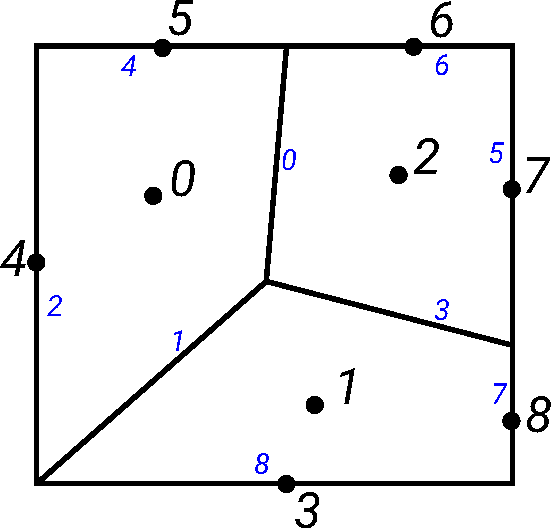
\includegraphics[width=0.25\linewidth]{extended_coll.pdf}
\caption{Расширенный набор точек коллокации}
\label{fig:extended_coll}
\end{figure}

На рис.~\ref{fig:extended_coll}.
представлена конечнообъёмная сетка, содержащая три ячейки
и девять граней. Индексация граней обозначена синими цифрами.
Всего три внутренних грани и шесть граничных.
Согласно стандартной методике конечных
объёмов сеточная функция
будет представлена массивом из трёх элементов.
В расширенном наборе будет девять точек коллокации (обозначены чёрными кругами и проиндексированы чёрными цифрами):
три соответствуют центрам ячеек и ещё шесть -- центрам граничных граней.

Пусть в области с рис.~\ref{fig:extended_coll} нужно решить
уравнение Пуассона \cref{eq:fvm_pois}.
Пусть на ниженей грани задано условие первого рода: $u = C$,
а на правой -- условие третьего рода: $\dsfr{u}{n} = \alpha u + \beta$.

\paragraph{Старый подход}
Согласно ранее рассмотренному методу конечных объёмов
аппроксимация задачи в ячейке с индексом 1 будет иметь следующий вид
$$
\frac{u_1 - u_0}{h_{10}}|\gamma_1|
+\frac{u_1 - u_2}{h_{12}}|\gamma_3|
+\frac{u_1 - C}{h_{13}}|\gamma_8|
+\frac{\alpha u_1 + \beta}{1 - \alpha h_{18}}|\gamma_7|
= V_1 f_1.
$$
Общая размерность матрицы СЛАУ при таком подходе будет
равна $3\times3$, а её элементы в 1-ой строке равны
$$
a_{10} = -\frac{|\gamma_1|}{h_{10}},  \quad
a_{12} = -\frac{|\gamma_3|}{h_{12}},  \quad
a_{11} = \frac{|\gamma_1|}{h_{10}}  + \frac{|\gamma_3|}{h_{12}} + \frac{|\gamma_8|}{h_{13}} + \frac{\alpha|\gamma_7|}{1 - \alpha h_{18}}.
$$
Справа в 1-ой строке будет стоять
$$
b_1 = V_1 f_1 + \frac{C |\gamma_8|}{h_{13}} - \frac{\beta |\gamma_7|}{1 - \alpha h_{18}}.
$$

\paragraph{Новый подход}
В расширенным набором точек коллокаций
матрица правой части будет иметь размерность $9\times9$.
Из них первые три будут собираться согласно классической процедуре
метода конечных объёмов, но учитывая наличие дополнитиельных точек коллокации в центрах
граничных граней. Так, 1-ое уравнение итоговой СЛАУ примет вид
$$
\frac{u_1 - u_0}{h_{10}}|\gamma_1|
+\frac{u_1 - u_2}{h_{12}}|\gamma_3|
+\frac{u_1 - u_3}{h_{13}}|\gamma_8|
+\frac{u_1 - u_8}{h_{18}}|\gamma_7|
= V_1 f_1.
$$
Остальные шесть уравнений будут представлять из себя
аппроксимацию граничных условий для соответствующих граней.
Так, 3-е уравнение будет соответствовать условию первого рода на грани $\gamma_8$:
$$
u_3 = C,
$$
а уравнение 8 -- условию третьего рода на грани $\gamma_7$:
$$
\frac{u_8 - u_1}{h_{18}} = \alpha u_8 + \beta
$$
Переводя рассмотренные уравнения в матричные коэффициенты, получим
следующие ненулевые коээфиициенты итоговой матрицы $\{a_{ij}\}$ и вектора правой части $\{b_i\}$. Для 1-ой строки
$$
a_{10} = -\frac{|\gamma_1|}{h_{10}},  \quad
a_{12} = -\frac{|\gamma_3|}{h_{12}},  \quad
a_{13} = -\frac{|\gamma_8|}{h_{13}},  \quad
a_{18} = -\frac{|\gamma_7|}{h_{18}},  \quad
a_{11} = -(a_{10} + a_{12} + a_{13} + a_{18}), \quad
b_1 = V_1 f_1,
$$
для 3-ей строки
$$
a_{33} = 1, \quad b_3 = C,
$$
для 8-ой строки
$$
a_{81} = -\frac{1}{h_{18}},  \quad
a_{88} = -a_{81} - \alpha, \quad
b_8  = \beta
$$

\subsection{Задание для самостоятельной работы}
\begin{enumerate}
\item
Решить задачу из п.~\ref{sec:hw_fvm2d}, 
с истинными граничными условиями первого рода,
и с граничными условиями первого рода, поставленными
через условия третьего рода.
\item
Убедится, что полученный ответ
с точностью то ошибки решения СЛАУ ($10^{-8}$)
совпадает с результатами, полученным
в двух предыдущих заданиях.
\item
Для постановки с условиями третьего рода
построить график максимального
отклонения граничного значения
полученного сеточной функции $\gvec{u}$ от точного решения в зависимости от выбранного $\eps^{-1}$ из \cref{eq:fvm_bc3_universal}
от точного решения:
$$
n_b = \max_{j > N_c} |u_j - u^e(\vec x_j)|,
$$
$N_c$ -- количество ячеек сетки, $j$ -- индекс граничных точек коллокации, $x_j$ -- координата точки коллокации.

\end{enumerate}

\paragraph{Рекомендации к программированию}
\begin{itemize}
\item
В структуру \cvar{DirichletFaces} необходимо добавить
поле \cvar{icol} -- индекс точки коллокации для текущей грани.
Нумерацию граничных точек коллокации нужно вести
начиная от \cvar{grid.n_cells()} согласно
порядку вектора \cvar{_dirichlet_faces}.
\item
Следует учитывать, что вектор неизвестных \cvar{_u} 
будет иметь длину, большую чем количество ячеек.
В частности, это может привести к ошибке сохранения в vtk.
Чтобы ограничить количество сохраняемых элементов вектора,
вызов сохранения необходимо осуществять с дополнительным параметром:
\begin{cppcode}
	VtkUtils::add_cell_data(_u, "numerical", filename, _grid.n_cells());
\end{cppcode}

\end{itemize}

\section{Лекция 9 (13.04)}

\subsection{Учёт скошенности сетки в двумерной МКО-аппроксимации}
\subsubsection{Уточнённая аппроксимация нормальной производной}
Ключевым моментом для аппроксимации оператора Лапласа
методом конечных объёмов является выражение нормально производной
по грани конечного объёма.
До сих пор мы пользовались соотношением \cref{eq:fvm_dudn_dudc},
которая на скошенных сетках приводила к большим численным погрешностям
и не давала желаемый второй порядок аппроксимации (см. задачу из п.~\ref{sec:hw_fvm2d}).
Для устранения этого недостатка распишем нормальную производную по грани более точно.

Для двумерного случая распишем градиент $u$ в системе координат,
образованной еодиничными векторами нормали $\vec n$ и касательной $\vec s = (-n_y, n_x)$
к грани $\gamma_{ij}$ (см. рисунок \figref{fig:fvm_grid}):
$$
\nabla u = \dfr{u}{n}\vec n + \dfr{u}{s} \vec s.
$$
С помощью значений функции в точках коллокации $i$ и $j$
мы можем аппроксимировать производную
$$
\left.\dfr{u}{c}\right|_{\gamma_{ij}} = \frac{u_j - u_i}{h_{ij}} + O(h^2)
$$
в центре грани $\gamma_{ij}$ вторым порядком точности как симметричную разность.
Эта производная есть проекция градиента функции $u$ на
вектор $\vec c$. Тогда можно записать:
$$
\dfr{u}{c} = \nabla u \cdot \vec c = \dfr{u}{n} \vec n \cdot \vec c + \dfr{u}{s} \vec s \cdot \vec c
 = \dfr{u}{n} \cos(\vecangle{n}{c}) + \dfr{u}{s} \sin(\vecangle{n}{c}).
$$
Отсюда выразим искомую производную
\begin{equation}
\label{eq:fvm_dudn_div}
\dfr{u}{n} = \dfr{u}{c} \frac{1}{\cos(\vecangle{n}{c})} - \dfr{u}{s} \tan(\vecangle{n}{c}).
\end{equation}
Для записи аппроксимации второго порядка нормальной производной
необходимо с заданной точностью аппроксимировать производную по касательной к грани.
В двумерном случае введём вспомогательные точки $\vec c^{+}$  и $\vec c^{-}$ как
показано на рисунке (\ref{fig:fvm_skew_example}). Тогда в центре грани запишем искомую симметричную разность
$$
\dfr{u}{s} = \frac{u^{+} - u^{-}}{|\vec c^+ - \vec c^-|} + O(h^2).
$$
Тогда получим аппроксимацию второго порядка искомой производной:
\begin{equation}
\label{eq:fvm_dudn_upm}
\dfr{u}{n} \approx \frac{u_j - u_i}{|\vec c_j - \vec c_i|} \frac{1}{\cos(\vecangle{n}{c})} - \frac{u^{+} - u^{-}}{|\vec c^+ - \vec c^-|}  \tan(\vecangle{n}{c}).
\end{equation}
Точки $c^{\pm}$ не являются точками коллокации, поэтому значения $u^{\pm}$ явно
присутствовать в аппроксимационной схеме не могут. Однако, их можно проинтерполировать
через значения $u$ в точках коллокации.

\subsubsection{Интерполяция значения функции во вспомогательных точках}
Для простой линейной интерполяции функции, заданной на двумерной плоскости,
необходимо три узловые точки, не лежащие на одной прямой.
Пусть двумя из этих трёх точек будут уже обозначенные $\vec c_i$ и $\vec c_j$.
Третью точку $\vec c_k$ будем выбирать из коллокации, 
соседних с временной точкой:
центров ячеек и центров граничных граней, которые содержат точку $\vec c^-$.

\begin{figure}[h!]
\centering
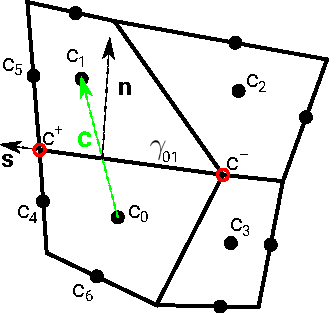
\includegraphics[width=0.25\linewidth]{fvm_skew_example.pdf}
\caption{Пример расположения вспомогательных точек (показаны красными кругами) для аппроксимации производной по грани}
\label{fig:fvm_skew_example}
\end{figure}

На примере с рис.~\ref{fig:fvm_skew_example} для точки $\vec c^-$ соседними будут точки $c_0, c_1, c_2, c_3$.
Точки $\vec c_0$ и $\vec c_1$ -- это первые две точки интерполяции (узлы $i$ и $j$ в предыдущих обозначениях).
Третью точку выберем как ближайшую к $\vec c^-$ из остальных, а именно $c_3$.
Для точки $\vec c^+$ третьей точкой будет $c_4$, выбранная аналогичным образом
из набора $c_0, c_1, c_4, c_5$.

Отметим, что для написания надёжного кода необходимо удостовериться,
что выбранная третья точка не лежит на одной прямой с двумя первыми.
И если лежит, то необходимо выбрать следующего кандидата.
А если кандидатов больше нет, то поиск необходимо продолжить
среди несоседних точек коллокации.

После того, как три узловые точки интерполяции
выбраны можно выразить вспомогательные значения
\begin{align*}
&u^- = C^-_i u_i + C^-_j u_j + C^-_k u_k,\\
&u^+ = C^+_i u_i + C^+_j u_j + C^+_s u_s,
\end{align*}
где коэффициенты интерполяции $C$ вычисляются следуя формуле
\cref{eq:simplex_interp_2d}. Например,
$$
C^-_i = \frac{|\triangle_{jk-}|}{\triangle_{ijk}|} =
\frac{
(\vec c_k - \vec c_j)\times(\vec c^- - \vec c_j)
}{
(\vec c_j - \vec c_i)\times(\vec c_k - \vec c_i)
}
$$
Подставив полученные интерполяционные соотношения в \cref{eq:fvm_dudn_upm},
получим аппроксимацию нормальной производной в виде линейную формы
\begin{equation}
\label{eq:fvm_dudn_linform}
\dfr{u}{n} \approx C_i u_i + C_j u_j + C_k u_k + C_s u_s.
\end{equation}
Коэффициенты которой равны
\begin{align*}
&C_i = -w_1 - (C_i^+ - C_i^-)w_2,
\\
&C_j = w_1 - (C_j^+ - C_j^-)w_2,
\\
&C_k = C_k^- w_2,
\\
&C_s = -C_s^+ w_2,
\\
&w_1 = \frac{1}{|\vec c_j - \vec c_i|\cos(\vecangle{n}{c})},
\\
&w_2 = \frac{\tan(\vecangle{n}{c})}{|\vec c^+ - \vec c^-|}
\end{align*}

\subsubsection{Производная по границе}
Из-за использования расширенного набора точек коллокации, 
процедура аппроксимации нормальной производной по граничной грани
ничем не отличается от аналогичной процедуры
для внутренней грани.
Так для точки коллокации $\vec c_4$
линейная форма, аппроксимирующая нормальную производную,
будет содержать значения $u_4, u_0, u_6, u_1$,
последние два из которых используются для интерполяции
вспомогательных точек.

Рассмотрим условие третьего рода \cref{eq:fvm_bc3} на стенке, соответсвующей
индексу коллокации $j$, соседней с ячейкой $i$.
C учётом \cref{eq:fvm_dudn_linform} получим:
\begin{equation*}
\dfr{u}{n} = C_i u_i + C_j u_j + C_k u_k + C_s u_s = \alpha u_j + \beta,
\end{equation*}
тогда $j$-ое уравнение СЛАУ будет иметь вид
\begin{equation}
\label{eq:fvm_bc3_skew_slae}
C_i u_i + (C_j - \alpha) u_j + C_k u_k + C_s u_s = \beta.
\end{equation}

\subsubsection{Сборка СЛАУ для уравнения Пуассона}
Рассмотрим процедуру сборки системы линейных уравнений для решения уравнения Пуассона.
Будем использовать цикл по граням по аналогии с \cref{eq:fvm_assem_internal}.
Ключевым моментом алгоритма будет являтся вычисление линейной формы
вида \cref{eq:fvm_dudn_linform}.
Отметим, что цикл по внутренним \cref{eq:fvm_assem_internal} и граничным \cref{eq:fvm_assem_bc_extended} граням
можно объединить в один цикл по всем граням. При этом следует
иметь ввиду, что этот цикл собирает уравнение внутри конечного объема
\cref{eq:fvm_pois_int}, и поэтому вносит изменения только
в строки, соответствующие центрам ячеек.
\begin{equation}
\label{eq:fvm_assem_internal_skew}
\begin{array}{ll}
\textbf{for } s \in\textrm{faces}                                & \textrm{-- цикл по всем граням}\\ 
\qquad i,j,k,s = \textrm{dn\_cells(s)}                           & \textrm{-- индексы точек коллокации для аппроксимации $\dsfr{u}{n}$}\\
\qquad v_i,v_j,v_k,v_s = \textrm{dn\_coefs(s)}                   & \textrm{-- коэф-ты линейной формы для аппроксимации $\dsfr{u}{n}$ }\\
\qquad a = \textrm{face\_area}(s)                                & \textrm{-- площадь грани}\\
\qquad \textbf{if } i \textrm{ is cell center }                  & \textrm{-- если $i$ -- коллокация для центра ячейки}\\
\qquad \qquad A_{ii} \minuseq  a\,v_i;                           & \textrm{-- $i$-ая строка матрицы (против нормали к грани)}\\ 
\qquad \qquad A_{ij} \minuseq  a\,v_j;                           & \\ 
\qquad \qquad A_{ik} \minuseq  a\,v_k;                           & \\
\qquad \qquad A_{is} \minuseq  a\,v_s;                           & \\
\qquad \textbf{endif}                                            & \\
\qquad \textbf{if } j \textrm{ is cell center }                  & \textrm{-- если $j$ -- коллокация для центра ячейки}\\
\qquad \qquad A_{ji} \pluseq a\,v_i;                             & \textrm{-- $j$-ая строка матрицы (по нормали к грани)}\\ 
\qquad \qquad A_{jj} \pluseq a\,v_j;                             & \\ 
\qquad \qquad A_{jk} \pluseq a\,v_k;                             & \\
\qquad \qquad A_{js} \pluseq a\,v_s;                             & \\
\qquad \textbf{endif}                                            & \\
\textbf{endfor}                                                  & \\
\end{array}
\end{equation}

В случае, если используются граничные условия второго или третьего рода,
та же процедура должна быть использована для выражения на границах \cref{eq:fvm_bc3_skew_slae} по аналогии с 
\cref{eq:fvm_assem_bc3_extended}.
\begin{equation*}
%\label{eq:fvm_assem_bc3_skew_extended}
\begin{array}{ll}
\textbf{for } s \in\textrm{bnd3}                         & \textrm{-- грани с условиями третьего рода}\\ 
\qquad i,j,k,s = \textrm{dn\_cells(s)}                   & \textrm{-- индексы точек коллокации для аппроксимации $\dsfr{u}{n}$}\\
\qquad v_i,v_j,v_k,v_s = \textrm{dn\_coefs(s)}           & \textrm{-- коэф-ты линейной формы для аппроксимации $\dsfr{u}{n}$ }\\
\qquad \textbf{if } j \textrm{ is cell center}           & \\
\qquad \qquad \textrm{swap}(i, j)                        & \textrm{-- переворачиваем нормаль. Теперь $j$ -- коллокация по грани} \\
\qquad \qquad v_i = -v_i, \quad v_j = -v_j               & \\
\qquad \qquad v_k = -v_k, \quad v_s = -v_s               & \\
\qquad \textbf{endif}                                    & \\
\qquad A_{ji} = C_i, \qquad A_{jj} = C_j-\alpha          & \\
\qquad A_{jk} = C_k, \qquad A_{js} = C_s                 & \\
\qquad b_{j} = \beta                                     & \\
\textbf{endfor}                                          & \\
\end{array}
\end{equation*}

\subsection{Задание для самостоятельной работы}
Решить двумерную задачу Пуассона с граничными условиями первого рода, аналогичную \ref{sec:hw_fvm2d},
но использовать поправку на скошенность.
Провести расчёт на сгущающихся сетках
и проиллюстрировать порядок аппроксимации
для структурированной, pebi и скошенной сетки.
Сравить графики сходимости с аналогичными, полученными в п.~\ref{sec:hw_fvm2d}.

\paragraph{Рекоммендации к программированию}
Для вычисления линейной формы \cref{eq:fvm_dudn_linform}
использовать класс \cvar{FvmLinformFacesDn}
из файла \ename{fvm/fvm_assembler.hpp}.

Объект этого класс необходимо собрать на этапе инициализации задачи.
Далее линейные формы для заданной грани вычисляются вызовом метода
\cvar{FvmLinformFacesDn::linear_combination(size_t iface)}.
Этот метод возвращает упорядоченную линейную комбинацию
из четырех (для двумерной задачи) слагаемых.
Получение индексов и коэффициентов линейной формы согласно алгоритму
\cref{eq:fvm_assem_internal_skew} осуществляется следующим образом
\begin{cppcode}
FvmLinformFacesDn faces_dn(grid);
for (size_t iface=0; iface < grid.n_faces(); ++iface){
	auto linform = faces_dn.linear_combination(iface);
	size_t i = linform[0].first;
	size_t j = linform[1].first;
	size_t k = linform[2].first;
	size_t s = linform[3].first;
	double vi = linform[0].second;
	double vj = linform[1].second;
	double vk = linform[2].second;
	double vs = linform[3].second;
}
\end{cppcode}



\section{Лекция 10 (20.04)}
\subsection{Учёт скошенности сетки в 3D}

\section{Лекция 11 (27.04)}
\subsection{Метод взвешенных невязок}
\subsection{Метод Бубнова--Галёркина}
\subsubsection{Степенные базисные функции}
\subsection{Метод конечных элементов}
\subsubsection{Узловые базисные функции}
\subsubsection{Одномерное уравнение Пуассона}
\subsubsubsection{Слабая интегральная постановка задачи}
\subsubsubsection{Линейный одномерный (пирамидальный) базис}

\section{Лекция 12 (04.05)}
\subsection{Поэлементная сборка конечноэлементных матриц}
\subsubsubsection{Элементные матрицы}
Матрица масс
\begin{equation}
\label{eq:fem_mass_matrix}
m^k_{ij} = \arint{\phi_i(\vec x) \phi_j(\vec x)}{E^k}{\vec x}
\end{equation}
Вектор нагрузок
\begin{equation}
\label{eq:fem_load_vector}
l^k_{i} = \arint{\phi_i(\vec x)}{E^k}{\vec x}
\end{equation}
Матрица жёсткости
\begin{equation}
\label{eq:fem_stiff_matrix}
s^k_{ij} = \arint{\nabla \phi_i \cdot \nabla \phi_j}{E^k}{\vec x}
\end{equation}

\section{Лекция 13 (11.05)}
\subsection{Вычисление элементных интегралов в параметрическом пространстве}
Будем вычислять элементные интегралы \cref{eq:fem_mass_matrix,eq:fem_stiff_matrix,eq:fem_load_vector}
в параметрическом пространстве $\vec \xi$.
Для этого введём преобразование координат $\vec x \rightarrow \vec \xi$ согласно п.\ref{sec:coo_transform}.
Интеграл для определения локальной матрицы масс \cref{eq:fem_mass_matrix} 
в параметрическом пространстве распишется согласно формуле \cref{eq:dxideta_integral}
\begin{equation}
\label{eq:mass_matrix}
m^k_{ij} = \arint{\tilde \phi^{(k)}_i(\vec \xi) \tilde \phi^{(k)}_j(\vec \xi)|J^{(k)}(\vec \xi)|}{\tilde E^k}{\vec \xi}
\end{equation}
Здесь $\tilde E^k$ -- параметрический образ конечного элемента $E^k$,
$J^{(k)}$ - Якобиан преобразования для $k$-ого элемента,
$\tilde \phi_{i}^{(k)}$ -- часть базисной функции $\phi_{c^k_i}$, определённая
в конечном элементе $E^k$ и заданная в параметрических координатах,
а $c^k_i$ -- глобальный индекс базисной функции, которая в $k$-ом элементе имеет локальный индекс $i$.
Таким образом справедливо
\begin{equation}
\nonumber
\tilde \phi_{i}^{(k)}(\vec \xi) = \phi_{c^k_i}(\vec x(\vec \xi))
\end{equation}
Локальный вектор нагрузок
\begin{equation}
\label{eq:load_vector}
l^k_{i} = \arint{\tilde \phi^{(k)}_i(\vec \xi)|J^{(k)}(\vec \xi)|}{\tilde E^k}{\vec \xi}
\end{equation}
Локальная матрица жёсткости
\begin{equation}
\label{eq:stiff_matrix}
s^k_{ij} = \arint{\nabla_{\vec x} \tilde \phi^{(k)}_i \cdot \nabla_{\vec x} \tilde \phi^{(k)}_j |J^{(k)}(\vec \xi)|}{\tilde E^k}{\vec \xi}
\end{equation}
Здесь $\nabla_{\vec x} \tilde \phi^{k}_i$ -- градиент локального базиса (заданного в параметрическом пространстве) по физическим координатам.
Для его вычисления следует воспользоваться формулами \cref{eq:vec_grad_dx}
\subsection{Двумерное уравнение Пуассона}
\subsubsubsection{Треугольный элемент. Линейный двумерный базис}
Матрица масс (из \cref{eq:mass_matrix}):
\begin{equation}
\label{eq:mass_matrix_lintri}
M^E_{ij} = \int\limits_0^1 \int\limits_0^{1-\xi} \phi_i(\xi, \eta) \phi_j(\xi, \eta) |J| \, d\eta d\xi =
\frac{|J|}{24}\left(
\begin{array}{ccc}
2 & 1 & 1 \\
1 & 2 & 1 \\
1 & 1 & 2
\end{array}
\right)
\end{equation}

\subsection{Разбор программной реализации МКЭ}
\label{sec:fem_programming}
\clisting{open}{"test/poisson_fem_solve_test.cpp"}
Численное решение уравнения Пуассона с граничными
условиями первого рода реализовано в файле
\ename{poisson_fem_solve_test.cpp}.
Будем рассматривать решение одномерной задачи с использованием пирамидальных базисов (тест \ename{[poisson1-fem-lintri]}).
В этом тесте определяется двумерная аналитическая функция
$$
f(x) = \sin(10 x^2),
$$
и формулируется уравнение Пуассона с граничными условиями первого рода, для которого эта функция является точным решением.
Далее уравнение Пуассона решается численно и полученный численный результат сравнивается
с точным ответом. Норма полученной ошибки печатается в консоль.

В функции верхнего уровня происходит построение одномерной
сетки, создание рабочего объекта, вызов решения с возвращением нормы полученной ошибки
и вывод данныех (сохранение решения в vtk-файл и печать нормы в консоль):
\clisting{pass}{"[poisson1-fem-linsegm]"}
\clisting{lines-range}{"Grid1D", "std::cout"}
Основная работа происходит в классе \cvar{TestPoissonLinearSegmentWorker}.

\subsubsection{Рабочий объект}
Класс \cvar{TestPoissonLinearSegmentWorker}
наследуется от \cvar{ITestPoisson1FemWorker}. В этом классе
сформулированы аналитические функции, служащие
правой частью, точным решением и условиями первого рода уравнения Пуассона.
А этот класс в свою очередь наследуется от \cvar{ITestPoissonFemWorker},
в котором и происходит решение уравнения.
\clisting{to-start}{}
\clisting{block}{"double ITestPoissonFemWorker::solve()"}
Для получения решения сначала собирается левая и правая
часть системы линеных уравнений,
потом происходит учёт граничных условий первого рода
, вызывается решатель системы уравнений и вычислитель нормы ошибки.

Функция сборки матрицы левой части реализует сборку глобальной матрицы жёсткости
через набор локальных матриц
\clisting{to-start}{}
\clisting{block}{"CsrMatrix ITestPoissonFemWorker::approximate_lhs() const"}
Основой для сборки служит специальный объёкт \cvar{_fem} класса
\cvar{FemAssembler} -- сборщик.
Этот объёкт сначала используется для задания шаблона итоговой матрицы,
потом в цикле по элементам вычисляются локальные матрицы и с
помощью метода этого класса \cvar{FemAssembler::add_to_global_matrix}
локальные матрицы добавляются в глобальную.

По аналогичной процедуре работает и сборка правой части \cvar{approximate_rhs}.

\subsubsection{Конечноэлементный сборщик}
Конечноэлементный сборщик \cvar{FemAssembler} -- основной класс, хранящий
всю информацию о текущей конечноэлементной аппроксимации: 
массив конечных элементов и их связность.
Эта информация подаётся ему при конструировании (реализация в файле \ename{cfd/fem/fem_assembler.hpp}).
\clisting{open}{"cfd/fem/fem_assembler.hpp"}
\clisting{lines-range}{"FemAssembler(", ");"}
Связность \cvar{tab_elem_basis} имеет формат \quo{элемент-глобальный базис} и
определяет глобальный индекс для каждого локального базисного индекса.
В рассматренных нами узловых конечных элементах базис связан с узлом сетки.
То есть эта таблица -- это связность локальной и глобальной нумерации узлов сетки для каждой ячейки сетки.

Конечноэлементный сборщик создаётся в методе
\cvar{TestPoissonLinearSegmentWorker::build_fem} итогового
рабочего класса (то есть сборщик специфичен для конкретной сетки
и конкретного выбора типов элементов). Далее он пробрасывается в конструктор базового рабочего класса.

\subsubsection{Концепция конечного элемента}
\clisting{open}{"cfd/fem/fem_element.hpp"}
Класс конечного элемента \cvar{FemElement} определён в файле
\ename{fem/fem_element.hpp} как
\clisting{block}{"struct FemElement"}
Главная задача объекта этого класса -- вычисление элементных матриц,
которые впоследствии используются сборщиком
для создания глобальных матриц.
Для расчёта элементных матриц в свою очередь требуется
\begin{itemize}
\item Геометрия элемента, включающая в себя правило отображения элемента из физической в параметрическую область,
\item Набор локальных базисных функций, заданных в параметрическом пространстве на указанной геометрии,
\item Непосредственно правило интегрирования в параметрической области.
\end{itemize}
Каждый из этих трёх алгоритмов определён через интерфейсы
\begin{itemize}
\item \cvar{IElementGeometry}
\item \cvar{IElementBasis}
\item \cvar{IElementIntegrals}
\end{itemize}
Определение конечного элемента заключается в задании конкретных реализаций этих интерфейсов.

\subsubsubsection{Определение линейного одномерного элемента}
\label{sec:linear_segment_assembly}.
Так, в рассматриваемом нами тесте \ename{"[poisson1-fem-linsegm]"}, используются только линейные одномерные элементы.
Используется следующее определение элемента:
\clisting{open}{"test/poisson_fem_solve_test.cpp"}
\clisting{pass}{"TestPoissonLinearSegmentWorker::build"}
\clisting{lines-range}{"geom =", "FemElement"}
Здесь последовательно определяются:
\begin{itemize}
\item
геометрия отрезка \cvar{geom} -- путём задания двух точек в физичекой плоскости \cvar{p0, p1},
\item
линейный одномерный базис \cvar{basis},
\item
правила интегрирования \cvar{integrals} по параметрическому отрезку $x \in [-1, 1]$
с использованием точных формул. Эти формулы зависят только от матрицы Якоби \cvar{jac} (размерности $1\times1$), которая
вычисляется с использованием геометрических свойств элемента
(в данном случае матрица Якоби постоянная, поэтому её можно вычислять в любой точке параметрической плоскости)
\end{itemize}
Этих трёх алгоритмов достаточно для полного определения конечного элемента \cvar{elem}.

\subsubsubsection{Геометрические свойства элемента}
\clisting{open}{"cfd/fem/fem_element.hpp"}
Интерфейс \cvar{IElementGeometry}, заданный в файле \ename{cfd/fem/fem_element.hpp},
определяет геометрические свойства элемента:
\clisting{block}{"class IElementGeometry"}
Для вычиселния элементных матриц главным геометрическим свойством
элемента является функция для вычисления матрицы Якоби (\cvar{jacobi}).
В простейших реализациях этого интерфейса для сиплексных геометрий
матрица Якоби постоянна для любой точки, то есть функция \cvar{jacobi} возвращает
один и тот же ответ вне зависимости от переданного аргумента.

Кроме того, этот интерфейс предоставляет функции преобразования координат из физического простравнства
в параметрическое и обратно: \cvar{to_parametric}, \cvar{to_physical}. А также задает центральную точку
в параметрическом пространстве \cvar{parametric_center}.

\subsubsubsection{Элементный базис}
Интерфейс для определения локального элементного базиса имеет вид
\clisting{open}{"cfd/fem/fem_element.hpp"}
\clisting{block}{"class IElementBasis"}
Этот интерфейс работает только с параметрическим пространстсвом
и определяет следующие методы:
\begin{itemize}
\item \cvar{size} -- количество базисных функций;
\item \cvar{parametric_reference_points} -- вектор из параметрических коордианат
      точек, приписанных к соответствующим базисам;
\item \cvar{value} -- значение базисных функций в заданной точке;
\item \cvar{grad} -- градиент (в параметрическом пространстве) базисных функций по заданным точкам.
\item \cvar{basis_type} -- тип базисной функции. До сих пор мы имели дело только с узловыми (\cvar{BasisType::Nodal})
      функциями.
\item \cvar{upper_hessian} -- верхняя часть матрицы Гессе (вторые производные базисных функций в заданной точке)
\end{itemize}

Конкретная реализация для линейного треугольного элемента \cvar{TriangleLinearBasis}
(в файле \ename{cfd/fem/elem2d/triangle_linear.cpp})
включает в себя линейный Лагранжев базис в двумерном пространстве согласно
\cref{eq:triangle_linear_basis}:
\clisting{open}{"cfd/fem/elem2d/triangle_linear.cpp"}
\clisting{block}{"TriangleLinearBasis::size"}
\clisting{block}{"TriangleLinearBasis::parametric_reference_points"}
\clisting{block}{"TriangleLinearBasis::value"}
\clisting{block}{"TriangleLinearBasis::grad"}


\subsubsubsection{Калькулятор элементных матриц}
Интерфейс \cvar{IElementIntegrals} предоставляет методы
для вычисления элементных матриц.
До сих пор были рассмотрены две элементные матрицы: матрица масс \cref{eq:mass_matrix} и матрица жёсткости \cref{eq:stiff_matrix}.
Для вычисления этих матриц используются функции \cvar{mass_matrix}, \cvar{stiff_matrix}.
Возвращают эти функции локальные квадратные матрицы с числом строк,
равным количеству базисов в элементе. 
Выходные матрицы развёрнуты в линейный массив. Так, для треугольного элемента
с тремя базисными функциями на выходе будет массив из девяти элементов:
$$
m_{00}, m_{01}, m_{02}, m_{10}, m_{11}, m_{12}, m_{20}, m_{21}, m_{22}.
$$

Два подхода к вычислению элементных интегралов: точное и численное интегрирование,
отражены в разных реализациях этого интерфейса.

До сих пор мы рассматривали только точное вычисление.
Точные формулы интегрирования зависят
от вида элемента. Так, для линейного одномерного элемента
аналитическое интегрирование реализовано в классе
\cvar{SegmentLinearIntegrals} в файле \ename{cfd/fem/elem1d/segment_linear.hpp},
а для линейного треугольного элемента -- 
\cvar{TriangleLinearIntegrals} в файле \ename{cfd/fem/elem2d/triangle_linear.hpp}
Все интегралы для этих симлексных элементов будут зависеть только от матрицы Якоби, которая и передётся этому классу в конструктор.
Например, вычисление матрицы масс (по \cref{eq:mass_matrix_lintri}) запрограммировано в виде
\clisting{open}{"cfd/fem/elem2d/triangle_linear.cpp"}
\clisting{block}{"mass_matrix()"}

\subsection{Задание для самостоятельной работы}
\label{sec:fem_programming_problem}
\begin{itemize}
\item
Показать второй порядок аппроксимации решения одномерного уравнения Пуассона
на линейных конечных элементах;
\item
Решить двумерное уравнение Пуассона с граничными условиями первого рода в квадтратной области на треугольной сетке.
Определить порядок аппроксимации двумерного уравнения Пуассона на треугольных элементах.
Для построения треугольных сеток различного разрешения использовать
скрипт \ename{trigrid.py}.
\item
Показать второй порядок аппроксимации решения двумерного уравнения Пуассона
на линейных треугольных конечных элементах;
\item
Сравнить сходимость на сгущающейся сетке конечноэлементного и конечнообъёмного решения
двумерного уравнения Пуассона на одних и тех же треугольных сетках.
Конечнообъёмное решение получать с использованием поправки на скошенность.
\end{itemize}

\paragraph{Рекомендации к программированию}
Для реализации двумерного решения
следует по аналогии с одномерным написать класс
\cvar{ITestPoisson2FemWorker},
в котором реализовать двумерные функции точного решения и правой части,
и наследуемый от него рабочий класс 
\cvar{TestPoissonLinearSegmentWorker},
в котором реализовать статическую функцию \cvar{build_fem}.
При реализации последней
использовать
алгоритмы для треугольников.
\begin{cppcode}
auto geom = std::make_shared<TriangleLinearGeometry>(p0, p1, p2);
auto basis = std::make_shared<TriangleLinearBasis>();
auto integrals = std::make_shared<TriangleLinearIntegrals>(geom->jacobi({}));
\end{cppcode}

\section{Лекция 14 (02.11)}

\subsection{Двухслойные схемы для нестационарных уравнений}

\subsubsection{Определение}

Рассмотрим дифференциальное уравнение вида

\begin{equation}
    \label{eq:nonstat_common}
    \dfr{u}{t} = f, \quad f(x, t) = g(x, t) - Lu(x, y)
\end{equation}
где $L$ -- произвольный пространственный дифференциальный оператор.
При использовании двухслойной схемы аппроксимации производная по времени записывается в
виде конечной разности с шагом $\tau$, которая может приближать производную
в одном из трёх моментов времени:

\begin{equation}
    \label{eq:nonstat_dt_appr}
    \begin{array}{llll}
        \dfrac{u(t+\tau) - u(t)}{\tau} = 
            & \quad \left.\ddfr{u}{t}\right|_{t}
            & + o(\tau)
            & -\text{ разность вперёд};\\[5pt]
        \phantom{a}
            & \quad \left.\ddfr{u}{t}\right|_{t+\tau}
            & + o(\tau)
            & -\text{ разность назад};\\[5pt]
        \phantom{a}
            & \quad \left.\ddfr{u}{t}\right|_{t+\frac{\tau}{2}}
            & + o(\tau^2)
            & -\text{ симметричная разность.}
    \end{array}
\end{equation}

Момент времени $t$ будем называть текущим временн<strong>ы</strong>м слоем,
момент $t + \tau$ -- следующим,
а момент $t+\tau/2$ -- промежуточным.
Считается, что
значение функции на текущий момент времени $u(t)$ известно, а
значение на следующий момент $u(t+\tau)$ подлежит определению.

\subsubsubsection{Явная схема}

При использовании разности назад уравнение \eqref{eq:nonstat_common}
в полудискретизованном (то есть дискретизованном только по времени, но не по пространству) виде
запишется как
\begin{equation*}
    \frac{u(x, t+\tau) - u(x)}{\tau} + L u(x, t) = g(x, t)
\end{equation*}
или, после переноса всех известных слагаемых вправо
\begin{equation}
    \label{eq:nonstat_explicit}
    u(x, t+\tau) = \left(E - \tau L\right) u(x, t) + \tau g(x, t).
\end{equation}
Здесь $E$ -- единичный оператор.
Схема \eqref{eq:nonstat_explicit} называется явной схемой
и имеет первый порядок точности.

\subsubsubsection{Неявная схема}

Выбрав разность назад из выражения \eqref{eq:nonstat_dt_appr}
полудискретизованная схема для уравнения \eqref{eq:nonstat_common} примет вид
\begin{equation*}
    \frac{u(x, t+\tau) - u(x)}{\tau} + L u(x, t+\tau) = g(x, t+\tau).
\end{equation*}
В результате преобразования получим неявную схему первого порядка точности
\begin{equation}
    \label{eq:nonstat_implicit}
    \left(E+\tau L\right) u(x, t+\tau) = u(x, t) + \tau g(x, t + \tau).
\end{equation}

\subsubsubsection{Схема Кранка--Николсон}

Подставим симметричную разность из \eqref{eq:nonstat_dt_appr}
в уравнение \eqref{eq:nonstat_common}. Формально получим
\begin{equation*}
    \frac{u(x, t+\tau) - u(x)}{\tau} + L u(x, t+\frac{\tau}{2}) = g(x, t+\frac{\tau}{2}).
\end{equation*}

Для определения выражения функций на промежуточном временном слое
распишем значение $u$ на текущем и следующем слоях в ряд Тейлора
относительно значения на момент $t+\tau/2$:
\begin{align*}
    u\left(t\right)      &= u\left(t+\frac{\tau}{2}\right) - \left.\frac{\tau}{2}\dfr{u}{t}\right|_{t+\frac{\tau}{2}} + o(\tau^2)\\
    u\left(t+\tau\right) &= u\left(t+\frac{\tau}{2}\right) + \left.\frac{\tau}{2}\dfr{u}{t}\right|_{t+\frac{\tau}{2}} + o(\tau^2)
\end{align*}
Взяв полусумму этих выражений получим аппроксимацию функции на промежуточном слое:
\begin{equation}
    \label{eq:nonstat_cn_appr}
    u\left(x, t + \frac{\tau}{2}\right) = \frac12u\left(x, t\right) + \frac12u\left(x, t+\tau\right) + o(\tau^2)
\end{equation}
Аналогичная запись справедлива и для свободного члена $g$.
Если оператор $L$ -- нестационарный или нелининый, то аппроксимацию \eqref{eq:nonstat_cn_appr}
следует записывать для всего выражения $Lu$:
\begin{equation*}
    \left(Lu\right)_{t+\frac{\tau}{2}} = \frac12\left(Lu\right)_{t} + \frac12\left(Lu\right)_{t+\tau} + o(\tau^2)
\end{equation*}


С учётом \eqref{eq:nonstat_cn_appr} симметричная разностная схема
запишется как
\begin{equation*}
    \frac{u(x, t+\tau) - u(x)}{\tau} + \frac12L u(x, t) + \frac12 L u(x, t + \tau) = \frac12 g(x, t) + \frac12 g(x, t+\tau)
\end{equation*}
или
\begin{equation}
    \label{eq:nonstat_cn}
    \left(E+\frac{\tau}{2} L\right) u(x, t+\tau) = \left(E - \frac{\tau}{2} L\right) u(x, t) + \frac{\tau}{2} \left(g(x, t) + g(x, t + \tau)\right).
\end{equation}
Такая схема называется схемой Кранка--Николсон и имеет второй порядок аппроксимации по времени.

В случае, если оператор $L$ зависит от времени, то
в левой части схемы \eqref{eq:nonstat_cn} его нужно
брать на следующем временном слое, а в правой -- на текущем.

\subsubsubsection{Обобщённая двухслойная схема}

Выражения
\eqref{eq:nonstat_explicit},
\eqref{eq:nonstat_implicit},
\eqref{eq:nonstat_cn}
можно записать в обобщённой форме
\begin{equation}
    \label{eq:nonstat_theta}
    \left(E+\theta\tau L\right) u(x, t+\tau) = \left(E + \left(\theta - 1\right)\tau L\right) u(x, t) + \left(1 - \theta\right) g(x, t) + \theta g(x, t + \tau).
\end{equation}
Коэффициент $\theta$ -- степень неявности схемы:
\begin{itemize}
\item $\theta = 0$ -- явная схема \eqref{eq:nonstat_explicit},
\item $\theta = 1$ -- полностью неявная схема \eqref{eq:nonstat_implicit},
\item $\theta = 1/2$ -- схема Кранка--Николсон \eqref{eq:nonstat_cn}.
\end{itemize}

Отметим, что только при $\theta = 1/2$ схема \eqref{eq:nonstat_theta} имеет второй порядок точности по времени.
Для других значений (в том числе промежуточных) схема будет иметь ошибку первого порядка $o(\tau)$.

\subsection{Схемы высокого порядка точности}
Существуют два подхода к построению схем дискретизации по времени произвольного высокого порядка:
первый из них предполагает использование нескольких временных слоев: $t+\tau, t, t-\tau, t-2\tau, ...$, второй -- использование
большого количества промежуточных точек на единственном временном отрезке: $t+c_i\tau, c_i\in[0, 1]$.
Первый подход используется для построения схем Адамса, второй -- схем Рунге--Кутта.

\subsubsection{Многослойные схемы. Схемы Адамса}
В общем виде многослойную расчётную схему можно записать в виде
\begin{equation}
\label{eq:nonstat_multilayer}
\sum\limits_{i=1}^{s} a_i u_i = \tau \sum\limits_{i=1}^{s} b_i f_i.
\end{equation}
Здесь нижние индексы функций использованы для указания временного слоя:
\begin{equation*}
\begin{aligned}
&u_i = u(x, t + (i+1-s)\tau),\\
&f_i = g(x, t + (i+1-s)\tau) - Lu_i,
\end{aligned}
\end{equation*}
а $s$ -- это общее количество используемых временных слоёв.
Значение всех функций на слоях $i<s$ считаются известными, а значение $u_s$ на последнем (текущем) слое подлежит определению.
Коэффициенты $a_i$. $b_i$ определяют конкретную схему.
Для однозначности принято задавать коэфиициет перед значением $u$ на текущем слое равным единице: $a_s = 1$.
Так, для двухслойной ($s=2$) схемы Кранка--Николсон \cref{eq:nonstat_cn} эти коэффициенты примут вид:
\begin{align*}
&a_1 = -1, \quad a_2 = 1,\\
&b_1 = 1/2, \quad b_2 = 1/2.
\end{align*}
Для того чтобы схема, записанная в общем виде \cref{eq:nonstat_multilayer}, была явной,
необходимо, чтобы выполнялось условие $b_s = 0$.

\subsubsubsection{Явные схемы Адамса--Башфорта}
Запишем интерполяционный полином для правой части уравнения \cref{eq:nonstat_common}
по значениям на предыдущих временных слоях $f_i, i<s$:
\begin{equation*}
p(t) = \sum\limits_{i=1}^{s-1}\left(f_i \prod\limits_{\substack{m=1\\m \neq i}}^{s-1} \frac{t - t_i}{t_m - t_i} \right).
\end{equation*}
Порядок аппроксимации этого полинома на единицу больше его степени. С учётом 
$t_{i+1} - t_{i} = \tau$ можно записать
\begin{equation*}
f(t) = p(t) + o(\tau^{s-1}).
\end{equation*}

Далее проинтегрируем уравнение по текущему временному отрезку: $[t_{s-1}, t_{s}]$:
\begin{equation*}
u_s - u_{s-1} = \sum_{i=1}^{s-1}\left( f_i \int\limits_{t_{s-1}}^{t_s} \prod \limits_{\substack{m=0\\m\neq i}}^{s-1} \frac{t - t_i}{t_m - t_i}\, dt \right).
\end{equation*}

Отсюда коэффициенты в общей форме \cref{eq:nonstat_multilayer} примут вид
\begin{equation*}
a_i = 
\begin{cases}
1,  &\quad i = s\\
-1, &\quad i = s-1\\
0,  &\quad i < s-1
\end{cases}
\qquad
b_i =
\begin{cases}
0, &\quad i = s\\[10pt]
\displaystyle\frac{1}{\tau}\int\limits_{t_{s-1}}^{t_s} \prod \limits_{\substack{m=0\\m\neq i}}^{s-1} \frac{t - t_i}{t_m - t_i}\, dt, &\quad i < s.
\end{cases}
\end{equation*}

Примеры трёх-, четырех- и пятислойной явных схем приведены ниже:
\begin{align*}
&\frac{u_3 - u_2}{\tau} = \frac{3f_2 - f_1}{2} + o(\tau^2),\\
&\frac{u_4 - u_3}{\tau} = \frac{23 f_3 - 16 f_2 + 5 f_1}{12} + o(\tau^3),\\
&\frac{u_5 - u_4}{\tau} = \frac{55 f_4 - 59 f_3 + 37 f_2 - 9 f_1}{24} + o(\tau^4).
\end{align*}

\subsubsubsection{Неявные схемы Адамса--Мультона}
Теперь снимем требование явности и запишем интерполяционный полином для правой части исходного уравнения \cref{eq:nonstat_common} с использованием $s$ точек:
\begin{equation*}
p(t) = \sum\limits_{i=1}^{s}\left(f_i \prod\limits_{\substack{m=1\\m \neq i}}^{s} \frac{t - t_i}{t_m - t_i} \right).
\end{equation*}
Тогда порядок аппроксимации этого полинома будем на единицу больше, чем для полинома явного метода.
Далее, проинтегрируем исходное уравенение по отрезку $t_{s-1}, t_s$ и получим коэффициенты общей формы \cref{eq:nonstat_multilayer}:
\begin{equation*}
a_i = 
\begin{cases}
1,  &\quad i = s\\
-1, &\quad i = s-1\\
0,  &\quad i < s-1
\end{cases}
\qquad
b_i =
\displaystyle\frac{1}{\tau}\int\limits_{t_{s-1}}^{t_s} \prod \limits_{\substack{m=0\\m\neq i}}^{s} \frac{t - t_i}{t_m - t_i}\, dt.
\end{equation*}

Двуслойная схема Адама--Мультона будет аналогична неявной двухслойной схеме \cref{eq:nonstat_implicit},
трёхслойная -- схеме Кранка--Николсон \cref{eq:nonstat_cn}. Примеры схемы высоких порядков представлены ниже:
\begin{align*}
&\frac{u_3 - u_2}{\tau} = \frac{5f_3 +  8 f_2 - f_1}{12} + o(\tau^3),\\
&\frac{u_4 - u_3}{\tau} = \frac{9 f_4 + 19 f_3 - 5 f_2 + f_1}{24} + o(\tau^4),\\
&\frac{u_5 - u_4}{\tau} = \frac{251 f_5 + 646 f_4 - 264 f_3 + 106 f_2 - 19 f_1}{720} + o(\tau^5).
\end{align*}

\subsubsection{Схемы Рунге-Кутта}
TODO

\subsection{Методы исследования устойчивости расчётных схем}
\label{sec:stability_analysis}

\subsubsection{Дискретизация по времени как итерационный процесс}

\subsubsubsection{Двухслойный итерационный процесс}

Простой двухслойный итерационный процесс определяется как
\begin{equation}
    \label{eq:nonstat_common_iter}
    u^{n+1} = A u^{n} + b,
\end{equation}
где $n$ -- индекс итерационного слоя,
$A$ -- оператор преобразования,
$b$ -- свободный член.

Определение значения функции на следующий момент времени $u(t+\tau)$ 
по двухслойной схеме \eqref{eq:nonstat_theta} можно представить как простой итерационный процесс \eqref{eq:nonstat_common_iter}, где
\begin{align*}
    A &= \left(E + \theta \tau L \right)^{-1} \left(E + (\theta - 1) \tau L \right), \\\\
    b &= \left(E + \theta \tau L \right)^{-1} \left( \theta g\left(x, t + \tau\right) + \left(1 - \theta\right) g\left(x, t\right) \right).
\end{align*}

Итерационный процесс называется сходящимся, если
\begin{equation*}
    \lim_{n=\infty} \left\lVert u^{n+1} - u^{n} \right\rVert = 0.
\end{equation*}

\subsubsubsection{Устойчивость итерационного процесса}
\label{sec:ScalarIter}

Рассмотрим два простых итерационных процесса,
имеющих на нулевом слое значение $u^0 = 1$:
\begin{align*}
    {\rm (I)}:\quad  &u^{n+1} = 2 u^{n} - 1, \\
    {\rm (II)} :\quad  &u^{n+1} = 0.5 u^{n} + 0.5.
\end{align*}
Оба этих процесса при выбранном начальном приближении, очевидно, сходятся.
На каждой итерации справделиво $u^n = 1$.
Возмутим начальное условие: пусть
\begin{equation*}
    u^0 = 1 + \eps,
\end{equation*}
и проведём итерации.
\begin{equation*}
    \def\arraystretch{1.7}
    \begin{array}{c|c|c}
        & {\rm (I)}  &  {\rm (II)} \\
        \hline
        u^1 & 1 + 2\eps & 1 + \dfrac{\eps}{2} \\
        \hline
        u^2 & 1 + 4\eps & 1 + \dfrac{\eps}{4} \\
        \hline
        u^3 & 1 + 8\eps & 1 + \dfrac{\eps}{8} \\
        \hline
        ... & & \\
        \hline
        u^\infty & \infty & 1 \\
    \end{array}
\end{equation*}

Видно, что процесс $\rm (I)$ теряет сходимость и стремится к бесконечности,
в то время, как процесс $\rm (II)$ сохраняет свои свойства.

Свойство итерационных процессов уменьшать малые возмущения называется устойчивостью.
В примере выше процесс $\rm (I)$ является неустойчивым, а процесс $\rm (II)$ -- устойчивым.

Нетрудно видеть, что для рассматриваемого скалярного итерационного процесса,
условие устойчивости запишется в виде $|A| \leq 1$.

\subsubsubsection{Источники возмущений}

На практике возникновение возмущений в решениях неизбежно:
они могут быть следствием ошибок дискретизации функций и операторов,
погрешностей решения СЛАУ, ошибок при проведении арифметических
операций на числах с плавающей точкой и т.д.
Поэтому любой итерационный процесс, используемый для решений
математических задач, должен быть устойчив.

Возникновение непреднамеренных ошибок вследствии компьютерного округления можно проиллюстрировать на примере
программы, в которой рассматривается сходящийся для любого начального условия, но неустойчивый итерационный процесс
\begin{equation*}
    u^{n+1} = 10 u^{n} - 9 u^{0}.
\end{equation*}

\begin{minted}[linenos=false]{c++}
double u0 = 0.625;
double u = u0;
for (int i=0; i<1000; ++i){
    u = 10*u - 9*u0;
}
std::cout << u << std::endl;
\end{minted}

Если начальное значение может быть точно представлено в
числах с плавающей точкой (путём конечной суммы степеней двойки),
то арифметическая ошибка не возникает.
Так, представленный выше код на выходе печатает ожидаемое $u=0.625$.
Потому что начальное приближение может быть разложено как $u^0 = 2^{-1} + 2^{-3}$.

Однако, если заменить начальное приближение на любое число,
которое не может быть записано точно во floating-point формате,
то процесс быстро уходит в бесконечность.
Например, для $u^0 = 0.626$ бесконечные (непредставимые в машинном формате) значения
появляются на 324-ой итерации,
а при переключении на работу в числах одинарной точности `float` -- уже на 46-ой.

\subsubsection{Матричный метод}

Итерационные процессы, возникающие при численном решении
дифференциальных уравнений сеточными методами, имеют матричную природу.
То есть оператор преобразования $A$ в выражении \eqref{eq:nonstat_common_iter} -- это матрица,
а функции $u$ и $b$ -- векторы-столбцы.

Как было показано выше, условием устойчивости скалярного итерационного процесса является неравенство $|A| \leq 1$.
Аналогом этого условия для матричного процесса является ограничение на спектральный радиус $S(A)$:
\begin{equation}
    \label{eq:nonstat_spectral_radius}
    S(A) = \max_j{ | \lambda_j | } \leq 1,
\end{equation}
где $\lambda_j$ -- собственные числа матрицы $A$.

Для некоторых видов матриц, возникающих при аппроксимации простейших дифференциальных уравнений,
собственные числа известны.

\subsubsubsection{Явная схема для нестационарного уравнения диффузии}
\label{sec:NonstatExpDiff}

Например, рассмотрим одномерное нестационарное уравнение диффузии с граничными условиями первого рода
\begin{align*}
    &\dfr{u}{t} = k\dfrq{u}{x},\\[5pt]
    &u(x, 0) = u_0(x),\\[5pt]
    &u(x_a, t) = u_a,\\[5pt]
    &u(x_b, t) = u_b.\\
\end{align*}
Используем явную дискретизацию по времени и аппроксимацию второго порядка по пространству.
Тогда разностная схема запишется в виде:
\begin{equation}
    \label{eq:nonstat_explicit_diff}
    \hat u_i = u_i + \gamma (u_{i-1} - 2 u_i + u_{i+1}), \quad i = \overline{1, N-1},
\end{equation}
где введено обозначение для значения функции на следующем временном слое $\hat u = u(t+\tau)$ и $\gamma = \tau k / h^2 $.
В матричном виде схема имеет вид
\begin{equation*}
    \hat u = A u, \quad
    A = \left(
        \begin{array}{cccccc}
            1      & 0          &           &            &           &        \\
            \gamma & 1-2\gamma  & \gamma    &            &           &        \\
                   & \gamma     & 1-2\gamma & \gamma     &           &        \\
                   &            & \ddots    & \ddots     & \ddots    &        \\
                   &            &           & \gamma     & 1-2\gamma & \gamma \\ 
                   &            &           &            & 0         & 1      
        \end{array}
    \right).
\end{equation*}
Первая и последняя строки этой матрицы -- следствие учёта граничных условий первого рода.

Собственные числа для полученной трёхдиагональной матрицы преобразования в правой части имеют вид
\begin{equation*}
    \lambda_j = 1 - 4\gamma\sin^2\left(\frac{j\pi}{2 N}\right), \quad j = \overline{1, N-1}
\end{equation*}
Тогда, исходя из выражения \eqref{eq:nonstat_spectral_radius}, запишем условие устойчивости
для явной схемы \eqref{eq:nonstat_explicit_diff}
\begin{equation*}
    \gamma \leq \frac12
\end{equation*}

\subsubsubsection{Неявная схема для нестационарного уравнения диффузии}\
\label{sec:NonstatImpDiff}

Аналогично, рассмотрим неявную схему
\begin{equation}
    \label{eq:nonstat_implicit_diff}
    \hat u_i - \gamma (\hat u_{i-1} - 2 \hat u_i + \hat u_{i+1}) = u_i, \quad i = \overline{1, N-1},
\end{equation}
В матричном виде
\begin{equation*}
    \hat u = A^{-1} u, \quad
    A = \left(
        \begin{array}{cccccc}
            1      & 0          &           &            &           &        \\
            -\gamma& 1+2\gamma  &-\gamma    &            &           &        \\
                   &-\gamma     & 1+2\gamma &-\gamma     &           &        \\
                   &            & \ddots    & \ddots     & \ddots    &        \\
                   &            &           &-\gamma     & 1+2\gamma &-\gamma \\ 
                   &            &           &            & 0         & 1      
        \end{array}
    \right).
\end{equation*}

Собственные числа такой матрицы имеют вид
\begin{equation*}
    \lambda_j = 1 + 4\gamma\sin^2\left(\frac{j\pi}{2 N}\right), \quad j = \overline{1, N-1}
\end{equation*}
Поскольку в правой части итерационного процесса используется матрица, обратная к $A$,
а собственные числа обратных матриц равны $1/\lambda_j$, то условие устойчивости
примет вид
\begin{equation*}
    \lambda_j \geq 1.
\end{equation*}
Очевидно, что оно выполняется всегда. Поэтому неявная схема \eqref{eq:nonstat_implicit_diff} безусловно устойчива.

\subsubsection{Метод дискретных возмущений}

Метод дискретных возмущений заключается
в использовании в качестве начального приближения
нулевого вектора, с возмущением $\eps$
в одном из узлов:
\begin{equation*}
    u^0 = \left(
        \begin{array}{c}
            0\\
            \vdots\\
            0\\
            \eps\\
            0\\
            \vdots\\
            0
        \end{array}
        \right)
\end{equation*}
и дальнейшем анализом
распространения этого возмущения с прохождением
по временным слоям.
Во многом этот метод аналогичен тому алгоритму,
по которому мы иллюстрировали устойчивость
простейшего скалярного итерационного процесса (\ref{sec:ScalarIter}).

\subsubsubsection{Явная схема против потока для уравнения переноса}
\label{sec:NonstatExpTran}

Для иллюстрации рассмотрим одномерное уравнение переноса
\begin{equation}
    \label{eq:nonstat_transport}
    \dfr{u}{t} + V\dfr{u}{x} = 0
\end{equation}
и явную противопоточную схему для него (при условии $V > 0$)
\begin{equation}
    \label{eq:nonstat_explicit_transport}
    \hat u_i = u_i - C \left(u_i - u_{i-1}\right),
\end{equation}
где число Куранта определено как $C = \tau V /h $.

Пусть $u_i = \eps$. Тогда
\begin{align*}
    & \hat u_i = (1 - C) \eps & \hence & \; 0 \leq C \leq 2,  \\[5pt]
    & \hat u_{i+1} = C \eps   & \hence & \; -1 \leq C \leq 1.
\end{align*}
Поскольку $C$ по определению больше нуля, то условием устойчивости для схемы $\eqref{eq:nonstat_explicit_transport}$
будет выражение
\begin{equation*}
    C \leq 1.
\end{equation*}

\subsubsection{Метод Неймана}

Запишем обратное преобразование Фурье для функции u(x):
\begin{equation*}
    u(x) = \int v(\kappa) e^{\imi \kappa x} \, d\kappa,
\end{equation*}
$\kappa$ -- волновое число, $\imi$ -- мнимая единица, $v(\kappa)$ -- Фурье образ исходной функции.

Зададим такое начальное возмущение, которое имеет единичную амплитуду 
на одной частоте, соответствующей волновому числу $\kappa_0$:
\begin{equation*}
    v(\kappa) = \delta(\kappa - \kappa_0),
\end{equation*}
$\delta(x)$ -- функция Дирака.
Кроме того, учтём, что $x_i = ih$.
Тогда выбранное начальное возмущение на одной выбранной частоте, взятое в $i$-ом узле, примет вид
\begin{equation}
    \label{eq:nonstat_neumann_decomp}
    u_i = e^{\imi i \theta}, \quad \theta = \kappa_0 h
\end{equation}
На следующем временном шаге это возмущение примет вид:
\begin{equation}
    \label{eq:nonstat_neumann_decomp_hat}
    \hat u_i = G e^{\imi i \theta}.
\end{equation}
$G$ -- коэффициент усиления. Он показывает во сколько раз
увеличилась амплитуда выбранного возмущения за один шаг по времени.
Для того, чтобы все возмущения затухали, необходимо
\begin{equation*}
    |G| \leq 1, \quad \forall \theta
\end{equation*}

\subsubsubsection{Неявная противопотоковая схема для уравнения переноса}
\label{sec:NonstatImpConv}

Для примера анализа устойчивости методом Неймана опять рассмотрим задачу $\eqref{eq:nonstat_transport}$,
но на этот раз рассмотрим чисто неявную аппроксимацию
\begin{equation}
    \label{eq:nonstat_implicit_transport}
    \hat u_i + C \left(\hat u_i - \hat u_{i-1}\right) = u_i.
\end{equation}

Подставим $\eqref{eq:nonstat_neumann_decomp}$, $\eqref{eq:nonstat_neumann_decomp_hat}$
\begin{equation*}
    G e(i) + C \left(G e(i) - G e(i-1)\right)= e(i). 
\end{equation*}
где для краткости введено обозначение
\begin{equation*}
    e(i) = e^{\imi \theta i}.
\end{equation*}
Поделим на $e(i)$ с использованием свойств этой степенной функции. Тогда

\begin{align*}
    & G + C G \left(1 - e(-1)\right)= 1 \quad \hence \\[10pt]
    & G = (1 + C (1 - e(-1)))^{-1}.
\end{align*}
По определению комплексной экспоненты имеем
\begin{equation*}
    e(-1) = \cos \theta - \imi \sin\theta.
\end{equation*}
Требуется показать, что $|G| \leq 1$. Отсюда
\begin{align*}
    & |1 + C (1 - \cos\theta + \imi\sin\theta)|  \geq 1 \quad \hence \\[10pt]
    & |1 + C (1 - \cos\theta) + C\imi\sin\theta)|^2 \geq 1 \quad \hence \\[10pt]
    & 1 + C^2(1-\cos\theta)^2 + 2C(1-\cos\theta) + C^2\sin^2\theta \geq 1 \quad \hence \\[10pt]
    & C^2(1-\cos\theta) + 2C + C^2(1+\cos\theta) \geq 0 \quad \hence \\[10pt]
    & C^2 + 2C \geq 0.
\end{align*}
По определению число Куранта больше 0, поэтому последнее выражение выполняется всегда.
Отсюда следует вывод, что неявная разностная схема вида $\eqref{eq:nonstat_implicit_transport}$
безусловно устойчива.

\subsubsubsection{Противопотоковая схема Кранка-Николсон для уравнения переноса}
\label{sec:NonstatCNConv}

Для того же самого уравнения $\eqref{eq:nonstat_transport}$
рассмотрим схему Кранка-Николсон $\eqref{eq:nonstat_cn_appr}$:
\begin{equation}
    \label{eq:nonstat_cn_transport}
    \hat u_i + \frac{C}{2} \left(\hat u_i - \hat u_{i-1}\right) = u_i - \frac{C}{2} \left(u_i - u_{i-1}\right).
\end{equation}
Так же
подставим $\eqref{eq:nonstat_neumann_decomp}$, $\eqref{eq:nonstat_neumann_decomp_hat}$
и поделим на $e(i)$:
\begin{align*}
    & G + \frac{C G}{2} \left(1 - e(-1)\right) = 1 - \frac{C}{2} \left(1 - e(-1)\right) \quad \hence \\[10pt]
    & G = \frac{1 - p}{1 + p}, \quad p = \frac{C}{2} \left(1 - e(-1)\right).
\end{align*}
Для выполнения условия устойчивости $|G| \leq 1$, необходимо
\begin{align*}
    & |1-p|^2 \leq |1+p|^2 \quad \hence \\[10pt]
    & (1 - \Re(p))^2 + \Im(p)^2 \leq (1+\Re(p))^2 + \Im(p)^2  \quad \hence \\[10pt]
    & \Re(p) \geq 0
\end{align*}
Здесь $\Re(p)$, $\Im(p)$ -- дейсвительная и мнимая часть комплексного числа.

Поскольку число Куранта больше нуля, то и действительная часть выражения $p$ неотрицательная для любого $\theta$.
\begin{equation*}
    \Re(p) = \frac{C}{2} \left(1 - \cos\theta\right) \geq 0.
\end{equation*}
Получаем, что схема видеа $\eqref{eq:nonstat_cn_transport}$ безусловно устойчива.

\subsubsubsection{Явная схема для уравнения нестационарной конвекции-диффузии}
\label{sec:NonstatExpConvDiff}

Рассмотрим уравнение конвекции-диффузии
\begin{equation}
    \label{eq:nonstat_convdiff}
    \dfr{u}{t} + V\dfr{u}{x} = k\dfrq{u}{x}
\end{equation}

Сначала напишем чисто явную схему второго порядка по пространству:
\begin{equation}
    \label{eq:nonstat_convdiff_explicit}
    \frac{\hat u_i - u_i}{\tau} + V\frac{u_{i+1} - u_{i-1}}{2h} = k\frac{u_{i+1} - 2 u_{i} + u_{i-1}}{h^2}
\end{equation}
Введем число Куранта $C = V \tau/h$ и параметр $\gamma = k \tau / h^2$. Тогда

\begin{equation*}
    \hat u_i = \left(\gamma - \frac{C}{2}\right) u_{i+1} + \left(\gamma + \frac{C}{2}\right) u_{i-1} + (1 - 2\gamma) u_i.
\end{equation*}
Далее подставим $\eqref{eq:nonstat_neumann_decomp}$, $\eqref{eq:nonstat_neumann_decomp_hat}$
\begin{equation*}
    G e(i) = \left(\gamma - \frac{C}{2}\right) e(i+1) + \left(\gamma + \frac{C}{2}\right) e(i-1) + (1 - 2\gamma) e(i).
\end{equation*}
Поделим на $e(i)$ с использованием свойств этой степенной функции. Тогда
\begin{equation*}
    G = \gamma(e(1) + e(-1)) - \frac {C}{2} (e(1) - e(-1)) + (1 - 2\gamma)
\end{equation*}
По определению комплексной экспоненты имеем
\begin{align*}
    e(1) &= \cos \theta + \imi \sin\theta,\\
    e(-1) &= \cos \theta - \imi \sin\theta,
\end{align*}
Отсюда
\begin{equation*}
    G = 2\gamma\cos\theta - \imi {C} \sin\theta + (1 - 2\gamma)
\end{equation*}
Запишем квадрат модуля комплексного числа $G$:
\begin{align*}
    |G|^2 = & \left(1 - 2\gamma(1-\cos\theta)\right)^2 + C^2 \sin^2\theta =\\
            & 1 + 4 \gamma^2(1-\cos\theta)^2 - 4\gamma(1-\cos\theta) + C^2 (1 - \cos^2\theta).
\end{align*}

Требование $|G| \leq 1$ эквивалентно $|G|^2 \leq 1$, или
\begin{align*}
    &1 + 4 \gamma^2(1-\cos\theta)^2 - 4\gamma(1-\cos\theta) + C^2 (1 - \cos^2\theta) \leq 1 \quad \hence \\[5pt]
    &4 \gamma^2(1-\cos\theta)^2 - 4\gamma(1-\cos\theta) + C^2 (1 - \cos^2\theta) \leq 0 \quad \hence \\[5pt]
    &4 \gamma^2(1-\cos\theta) - 4\gamma + C^2 (1 + \cos\theta) \leq 0 \quad \hence \\[5pt]
    &(C^2 - 4 \gamma^2) \cos\theta +4\gamma^2 - 4\gamma + C^2 \leq 0
\end{align*}

Поскольку неравенство должно выполняться для всех $\theta$,
а полученное выражение линейно зависит от $\cos\theta$, то будет достаточно рассмотреть два экстремальных значения косинуса,
из которых окончательно запишем два условия устойчивости для явной дискретизации уравнения конвекции-диффузии вида \eqref{eq:nonstat_convdiff_explicit}:
\begin{equation}
    \label{eq:nonstat_convdiff_explicit_cond}
    \begin{array}{lcl}
        \cos\theta = 1  & \hence & C \leq \sqrt{2\gamma}, \\
        \cos\theta = -1 & \hence & \gamma \leq 1/2.
    \end{array}
\end{equation}

Обычно вместо первого из условий \eqref{eq:nonstat_convdiff_explicit_cond} применяют
более жёсткое (в случае $2\gamma < 1$) условие
\begin{equation*}
    C \leq 2\gamma,
\end{equation*}
которое с учётом определений сводится к условию на шаг по пространству, формулируемому в терминах сеточного числа Рейнольдса $\Ren_c$:
\begin{equation*}
    \frac{V h}{k} \equiv \Ren_c \leq 2.
\end{equation*}

\subsubsubsection{Неявная схема для уравнения нестационарной конвекции-диффузии}
\label{sec:NonstatImpConvDiff}

Аналогичным образом рассмотрим неявную диффузии схему для уравнения \eqref{eq:nonstat_convdiff} вида
\begin{equation}
    \label{eq:nonstat_convdiff_semi_implicit}
    \frac{ \hat u_i - u_i}{\tau} + V\frac{ u_{i+1} - u_{i-1}}{2h} = k\frac{\hat u_{i+1} - 2 \hat u_{i} + \hat u_{i-1}}{h^2}
\end{equation}

Подставляя представление для возмущения с волновым числом $\theta$, получим
\begin{equation*}
    G = \frac{1 - \imi C \sin\theta}{1 - 2\gamma(\cos\theta - 1)}
\end{equation*}

Для устойчивости необходимо
\begin{align*}
    & |1 - \imi C \sin\theta|^2 \leq |1 - 2\gamma(\cos\theta - 1)|^2 \quad \hence \\[10pt]
    & 1 + C^2\sin^2\theta \leq 1 + 4\gamma^2(1 - \cos\theta)^2 + 4\gamma(1-\cos\theta) \quad \hence \\[10pt]
    & C^2(1 + \cos\theta) \leq 4\gamma^2(1 - \cos\theta) + 4\gamma \quad \hence \\[10pt]
    & \cos\theta(C^2 + 4\gamma^2) + C^2 - 4\gamma - 4\gamma^2 \leq 0
\end{align*}
Наибольшего значения выражение слева достигает при $\theta = 0$. Тогда единственное условие устойчивости 
примет вид
\begin{equation*}
    C \leq \sqrt{2\gamma}.
\end{equation*}

\subsubsection{Общие рекомендации к выбору устойчивых расчётных схем}
Теоретический анализ условий устойчивости возможен
лишь для простейших уравнений с постоянными шагами дискретизации.
В практических приложениях, имеющих дело, как правило,
с неструктурированными сетками и сложными нелинейными системами уравнений,
параметры устойчивого счёта приходится определять эмпирически.
Однако, такой теоретический анализ позволяет выделить принципы, которыми
следует руководствоваться для построения устойчивых схем.

{\bf Неявные схемы более устойчивы, чем явные}
\begin{itemize}
\item
Это можно видеть, сравнив результаты анализа
для безусловно устойчивой неявной схемы (\ref{sec:NonstatImpDiff}) для уравнения диффузного переноса и
для условно устойчивой явной схемы (\ref{sec:NonstatExpDiff}).
\item
Для уравнения переноса с разностью против потока
явная (\ref{sec:NonstatExpTran}) схема условно устойчива, в то время как
неявная (\ref{sec:NonstatImpConv}) -- устойчива безусловно.
\item
Даже если только часть схемы неявная, это повышает устойчивость.
Так,  явная (\ref{sec:NonstatExpConvDiff}) схема для уравнения конвекции-диффузии
имеет два условия устойчивости, в то время как
схема, неявная по диффузии (\ref{sec:NonstatImpConvDiff}) -- только одно.
\item
Аналогично,  явная (\ref{sec:NonstatExpTran}) схема против потока для
уравнения переноса условно устойчива,
а схема Кранка-Николсон (\ref{sec:NonstatCNConv}) для того же уравнения устойчива при любых параметрах.
\end{itemize}

{\bf Конвективное слагаемое провоцирует неусточивость, а диффузионное -- напротив, добавляет устойчивость}
\begin{itemize}
\item
Так, схемы с центральными разностями для уравнения конвекции-диффузии
(и явная (\ref{sec:NonstatExpConvDiff}), и полунеявная (\ref{sec:NonstatImpConvDiff})),
условно устойчивы. Явная схема с центральными разностями для чистого уравнения переноса всегда неустойчива.
В последнем можно убедится, подставив $k=0$ в условия устойчивости для уравнений конвекции-диффузии.
\end{itemize}

\subsection{Программная реализация схемы для уравнения переноса}

\subsubsection{Постановка задачи}
Рассматриваются три схемы по времени для противопотоковой аппроксимации уравнения переноса \eqref{eq:nonstat_transport}: 
\begin{itemize}
\item явная схема \eqref{eq:nonstat_explicit_transport} (тест называется \cvar{[transport1-explicit]}),
\item неявная схема \eqref{eq:nonstat_implicit_transport} (\cvar{[transport1-implicit]}),
\item схема Кранка--Николсон \eqref{eq:nonstat_cn_transport} (\cvar{[tranport1-cn]}).
\end{itemize}

Уравнение решается на отрезке $x\in[0, 1]$ с единичной скоростью $V = 1$
на сетке из 1000 ячеек. Временные итерации продолжаются до момента времени $t = 0.5$.

Начальным условием является функция вида
\begin{equation*}
    u(x, 0) = e^{-x^2/\sigma^2}, \quad \sigma = 0.1
\end{equation*}
Точное решение уравнения, с которого будут сниматься граничные условия и производится сравнения полученного численного решения,
запишется как
\begin{equation*}
    u(x, t) = u(x - t, 0) = e^{-(x-t)^2/\sigma^2}.
\end{equation*}

На каждом шаге по времени функция сохраняется в vtk-формате.
В конце выводится значение отклонения от точного решения на конечный момент времени.

В качестве цели решения обозначим построение решения и визуальное сравнение решений
при числе $C=0.9$ по трём разным схемам.
А также построение графика сходимости отклонения точного решения
от численного при изменении числа Куранта и фиксированном шаге по пространству
(то есть сходимость при уменьшении шага по времени).

Программы реализованы в файле \ename{transport_solve_test.cpp}.
\clisting{open}{"test/transport_solve_test.cpp"}

\subsubsection{Функция верхнего уровня}

Для всех трёх программ функция верхнего уровня имеет один и тот же вид.
Рассмотрим на примере первой из них:
\clisting{line}{"[transport1-explicit]"}

В начале происходит установка параметров численной схемы:
\begin{itemize}
\item конечного момента времени,
\item скорости переноса,
\item длины расчётной области,
\item разбиения по пространству,
\item числа Куранта
\end{itemize}

\clisting{lines-range}{"const double", "Cu"}

Далее вычисляются используемые шаги:
\begin{itemize}
\item шаг по пространству (из длины области и разбиения),
\item шаг по времени (из шага по пространству и числа Куранта)
\end{itemize}

\clisting{lines-range}{"double h", "double tau"}

Потом устанавливается рабочий класс, в котором будет производится решение
\clisting{line}{"TestTransport1WorkerExplicit worker"}

Конструируется класс, используемый для связного сохранения
полей на разные моменты времени.
Этот класс создаёт \ename{transport1-explicit.vtk.series}
со списком всех сохранённых полей и отнесёнными к ним моментами времени,
который можно впоследствии открыть в Paraview и использовать
функции анимации для воспроизведения поведения решения во времени.
\clisting{line}{"VtkUtils::TimeSeriesWriter writer(\"transport1-explicit\");"}
Далее нужно в этот класс сохранить решение на начальный момент времени.
Для этого туда сначала добавляется запись о нулевом моменте времени
\clisting{line}{"out_filename"}
В переменную \cvar{out_filename} записывается конкретное
имя vtk-файла, куда следует сохранить решение.
Уже это имя используется для сохранения решения на текущий (начальный) момент времени.
\clisting{line}{"out_filename"}

Далее начинается цикл по времени,
продолжающийся до тех пор, пока внутреннее время решателя
не достигнет конечного
\clisting{line}{"while"}

Внутри вызывается функция решения, которая продвигает
внутреннее время решателя на $\tau$, обновляет
актуальное состояние вектора решения
и возвращает текущую норму.
\clisting{line}{"norm"}

Потом повторяется процедура сохранения
текущего состояния решателя
\clisting{lines-range}{"out_filename", "save_vtk"}

После завершения цикла в консоль печатается
установленное разбиение по времени и
полученное отклонение от точного решения
на конечный момент времени 
\clisting{line}{"cout"}

\subsubsection{Расчётные функции}

Три класса-решателя для трёх заявленных задач:
\cvar{TestTransport1WorkerExplicit},
\cvar{TestTransport1WorkerImplicit},
\cvar{TestTransport1WorkerCN}
наследуются от одного абстрактного класса
\cvar{ATestTransport1Worker}. В этом
абстрактном классе реализованы
все общие для всех решателей функции:
создание сетки, сохранение в vtk,
расчёт нормы, продвижение по времени.

Этот класс также хранит в себе параметры, полностью определяющие текущее состояние решения:
\begin{itemize}
\item расчётную сетку,
\item шаг по времени (это параметр, производный от сетки, он сохранён в отдельное поле для удобства расчётов),
\item вектор решения на текущий момент,
\item текущее время.
\end{itemize}

Эти поля хранятся в `protected` секции, таким образом
все производные классы имеют к этим полям полный доступ.
\clisting{to-start}{}
\clisting{lines-range}{"protected:", "_time"}

Функция решения, также реализована в абстрактном классе.
Она продвигает текущее время и вызывает
виртуальный метод \cvar{impl_step}, который
изменяет значение вектора решения, а в конце вызывает
функцию вычисления ошибки.
\clisting{to-start}{}
\clisting{block}{"double step"}

Функция \cvar{impl_step} уже зависит от конкретной схемы и реализована в
производных классах

\subsubsubsection{Явная схема}

\clisting{to-start}{}

Её решатель реализован в классе \cvar{TestTransport1WorkerExplicit}. Рабочая функция по порядку:
\begin{itemize}
\item копирует текущий вектор значений во вспомогательный вектор \cvar{u_old}.
      Этот шаг добавлен сюда для ясности. Вообще говоря, его можно было избежать.
\item устанавливает граничное условие в левой точке
\item далее в цикле по точкам реализует расчётную схему \eqref{eq:nonstat_explicit_transport}.
\end{itemize}

\clisting{pass}{"TestTransport1WorkerExplicit"}
\clisting{block}{"impl_step"}

\subsubsubsection{Неявная схема}
Её решатель реализован в классе \cvar{TestTransport1WorkerImplicit}.
Поскольку здесь для нахождения решения требуется решить СЛАУ, то
порядок действий включает в себя:
\begin{itemize}
\item формирование класса-решателя.
\item формирование столбца свободных членов
\item вызова функции решения СЛАУ для найденного столбца правой части. Ответ записывается
      во внутреннее поле класса \cvar{_u}
\end{itemize}

\clisting{block}{"impl_step"}

Для построения и инициализации решателя необходимо
собрать матрицу правой части системы уравнений \eqref{eq:nonstat_implicit_transport}.
Матрица зависит от шага по времени (через число Куранта), при этом шаг по времени является
аргументом функции \cvar{build_solver}, которая приходит от пользователя решателя через аргумент функции \cvar{step()}`.

Таким образом, в логике работы приложения, нам придётся пересобирать матрицу на каждой временной итерации.
При этом, почти всегда шаги по времени постоянны для временных слоёв. То есть одну и ту же операцию (сборку матрицы)
при одним и тех же аргументах (шаге по времени) придётся повторять. 

Поскольку сборка матрицы -- дорогая операция, то результат работы
функции \cvar{build_solver} мы кэшируем (сохраняем во внутреннее поле класса \cvar{_solver}).
С тем чтобы на следующем временном слое в случае, если шаг по времени не изменился (\cvar{_last_used_tau == tau}),
просто вернуть ответ, посчитанный ранее.
\clisting{block}{"build_solver"}

Сама сборка двухдиагональной матрицы происходит в функции \cvar{build_lhs}.
В первой и последней строке учитываются граничные условия, а строки, соответствующие внутренним узлам,
заполняются согласно схеме \eqref{eq:nonstat_implicit_transport}
\clisting{block}{"build_lhs"}

Сборка правой части СЛАУ происходит в функции \cvar{build_rhs}.
Согласно схеме \eqref{eq:nonstat_implicit_transport}
правый столбец равен значению функции на предыдущем временном слое.
В коде мы создаём столбец \cvar{rhs} как копию вектора \cvar{_u}.
А далее переписываем первый и последний элемент с тем, чтобы
учесть граничные условия.
\clisting{block}{"build_rhs"}

\subsubsubsection{Схема Кранка-Николсон}
Её решатель реализован в классе \cvar{TestTransport1WorkerCN}.

По аналогии с предыдущей программой, здесь требуется
решить СЛАУ, возникающую из схемы \eqref{eq:nonstat_cn_transport}.
Таким образом, вся логика работы этого класса (включая кэширование решателя) повторяет логику
работы рассмотренного ранее класса для чисто неявной схемы \cvar{TestTransport1WorkerImplicit}.
Отличаются эти классы только реализацией функций построения матрицы и
правой части. Поэтому настоящий класс наследуется от \cvar{TestTransport1WorkerImplicit}
\clisting{line}{"TestTransport1WorkerCN"}
и переопределяет только функции 
сборки левой части \eqref{eq:nonstat_cn_transport} с учётом граничных условий
\clisting{block}{"build_lhs"}
и правой части \eqref{eq:nonstat_cn_transport} с учётом граничных условий
\clisting{block}{"build_rhs"}

\subsubsection{Анализ результатов работы}

Сравнение полученных ответов (по явной и неявной схемам) с точным решением представлено на \figref{fig:transport1_solution}.
\begin{figure}[h]
\centering
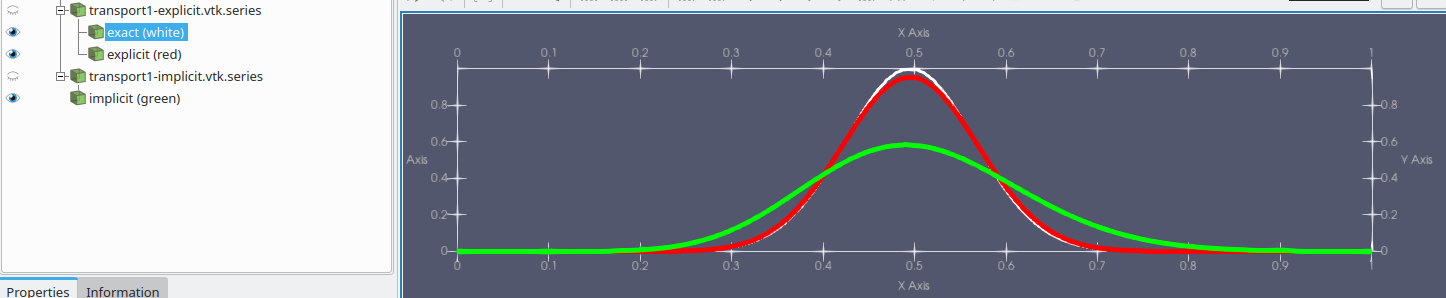
\includegraphics[width=1.0\linewidth]{transport1_solution.png}
\caption{Сравнение точного (белая линия) решения и численных решений по явной (красная) и неявной (зелёная) схемам}
\label{fig:transport1_solution}
\end{figure}

Чтобы получить такую картинку необходимо открыть в
Paraview сгенерированные в результате работы программ
выходные файлы \ename{transport1_explicit.vtk.series}
и \ename{transport1_implicit.vtk.series}
И далее проделать преобразования, описанные в пункте \ref{sec:paraview-1d}.

Для построения графиков сходимости, необходимо преобразовать
написанные программы, запустив цикл по различным значениям числа Куранта
\begin{minted}[linenos=false]{c++}
for (double Cu: { ... }){
    // solution
    ...

    std::cout << 1.0/tau << " " << norm << std::endl;
}
\end{minted}
и построить график полученной таблицы в логарифмических осях.
При задании диапазона изменений $C$ следует учитывать, что явная схема устойчива только при $C \leq 1$,
в то время как две другие схемы безусловно устойчивы.

Графики сходимости с уменьшением шага по времени
представлены на \figref{fig:transport1_norms}.

\begin{figure}[h]
\centering
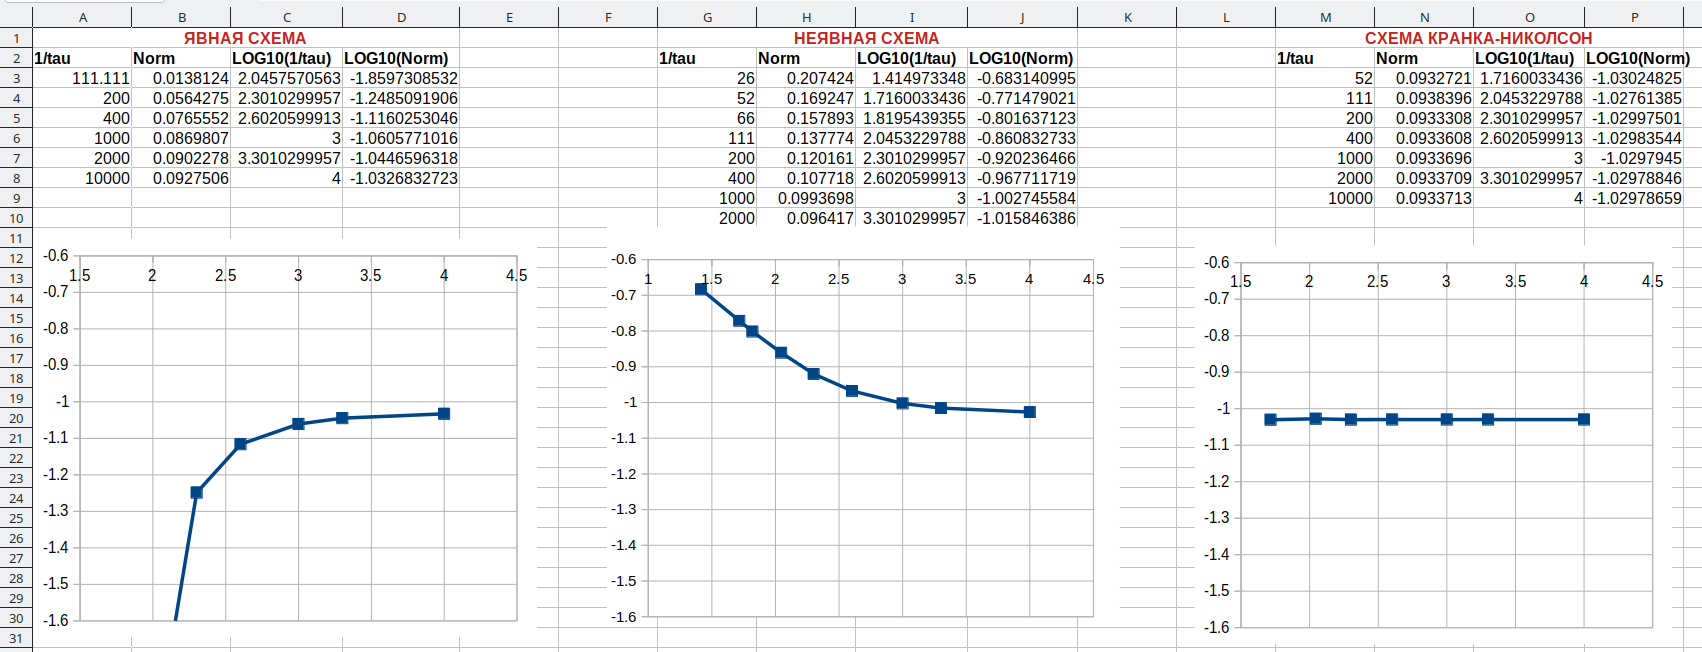
\includegraphics[width=1.0\linewidth]{transport1_norms.png}
\caption{Сходимость решения уравнения переноса с уменьшением $\tau$}
\label{fig:transport1_norms}
\end{figure}

Видно, что для явной схемы с уменьшением шага по времени
ответ отдаляется от точного, а для неявной -- наоборот, приближается.

Это объясняется тем, что в случае явной схемы
ошибки по времени и по пространству имеют разный знак
и (в случае их равенства) компенсируют друг друга.
А для неявной эти ошибки имеют одинаковый знак.

В пределе (с минимальным шагом по времени) все три схемы
сходятся к одной и той же ошибке (ошибке схемы по пространству).


\subsection{Задание для самостоятельной работы}
\subsubsection{Постановка задачи}
Написать двумерный решатель для уравнения переноса
\begin{equation*}
    \dfr{u}{t} + U \dfr{u}{x} + V \dfr{u}{y} = 0.
\end{equation*}

Решение проводить в квадрате $x,y\in[-1,1]$.

Требуется
\begin{itemize}
\item расчитать и нарисовать в Paraview нестационарное решение (см. \ref{sec:paraview-2d});
\item построить график, иллюстрирующий увеличение нормы ошибки
      с продвижением по времени;
\item исследовать устойчивость схемы. Эмпирическим путём выяснить,
      какое максимально возможный шаг по времени можно брать
      при фиксированном разбиении по пространству;
\item построить график, иллюстрирующий сходимость нормы
      ошибки при уменьшении шага по времени при фиксированном разбиении
      по пространству.
\end{itemize}

\subsubsubsection{Тестовый пример 1}
На этапе первичного тестирования использовать
значения скорости
\begin{equation*}
    U = 1, \quad V = 0.
\end{equation*}

А в качестве начального решения брать простой "столбик" (\figref{fig:transport1_work_01})
\begin{equation*}
    u(x,y,0) = u_0(x, y) = \begin{cases}
        1, & \; -1\leq x \leq -0.8, \; -0.1 \leq y \leq 0.1, \\
        0, & \; \text{иначе}.
    \end{cases}
\end{equation*}

\begin{figure}[h]
\centering
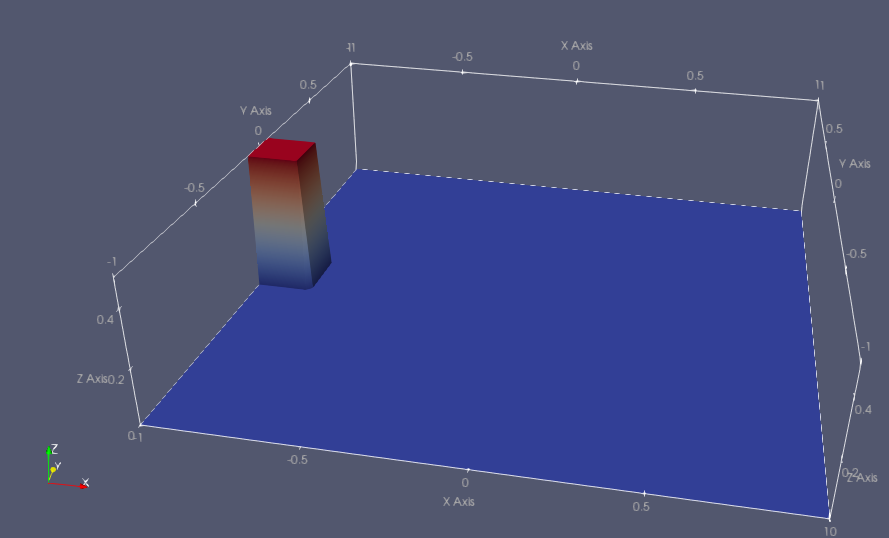
\includegraphics[width=1.0\linewidth]{transport1_work_01.png}
\caption{Начальные условия для первого тестового примера}
\label{fig:transport1_work_01}
\end{figure}

Точным решением будет функция
\begin{equation*}
    u^e(x, y, t) = u_0(x-t, y)
\end{equation*}

То есть этот столбик будет двигаться вправо с единичной
скоростью и за время 2 полностью покинет расчётную область.

\subsubsubsection{Тестовый пример 2}

После того, как этот тест будет пройден,
использовать постановку с непостоянной по пространству скоростью
\begin{equation*}
    U(x, y) = -y, \quad V(x, y) = x.
\end{equation*}

и начальным решением вида (\figref{fig:transport1_work_02})
\begin{align*}
    &r_0(x, y) = \sqrt{(x - 0.5)^2 + y^2}; \; \sigma = 0.05;\\
    &u(x, y, 0) = u_0(x, y) = e^{-r_0^2(x, y)/\sigma^2}
\end{align*}

\begin{figure}[h]
\centering
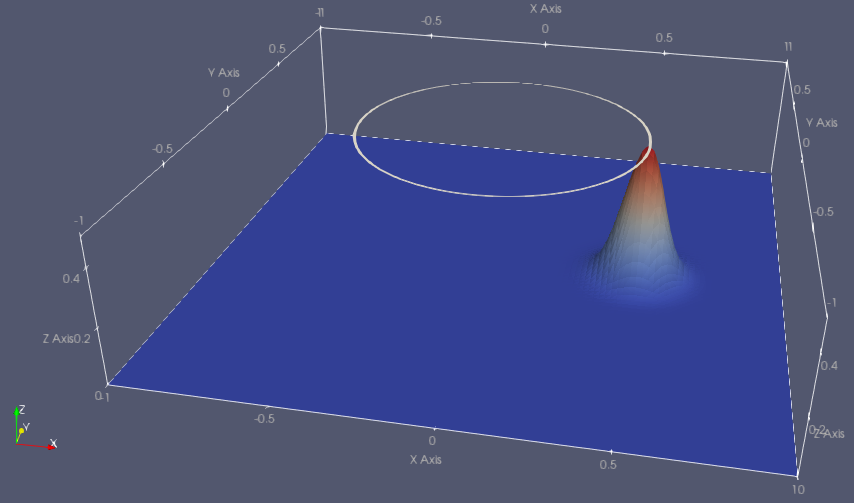
\includegraphics[width=1.0\linewidth]{transport1_work_02.png}
\caption{Начальные условия для второго тестового примера}
\label{fig:transport1_work_02}
\end{figure}

В процессе решения этот "холмик" будет
двигаться по окружности, описывая полный оборот за время $t=4\pi$.

Точное решение на момент времени $t$ будет иметь вид
\begin{align*}
  	& x_c(t) =  0.5\cos(0.5 t); \\
    & y_c(t) =  0.5\sin(0.5 t); \\
    & r(x, y, t) = \sqrt{(x - x_c(t))^2 + (y - y_c(t))^2};  \\
    & u^e(x, y, t) = e^{-r^2(x, y, t)/\sigma^2}
\end{align*}


\subsubsection{Расчётная схема}

Использовать противопотоковую явную схему:
\begin{equation*}
    \frac{\hat u_k - u_k}{\tau}
        + |U_k| \frac{u_k - u_{\upx{k}}}{h_x}
        + |V_k| \frac{u_k - u_{\upy{k}}}{h_y} = 0
\end{equation*}

Здесь $\upx{k}$, $\upy{k}$ -- 
значения индексов, расположенных против потока
отностительно узла $k$ в направлениях $x$ и $y$ соответственно.

Поскольку скорость в настоящей постановке непостоянная и зависит от точки пространства,
то вычислять индекс узла, расположенного против потока
приходится в зависимости от значения скорости.
С использованием ранее введёных алгоритмов перехода
от парных (i, j) индексов к сквозному индексу $k$ \eqref{eq:tasks_ij2k} и обратно \eqref{eq:tasks_k2ij} запишем
\begin{align*}
    & i = i[k]; \\
    & j = j[k]; \\
    & \upx{k} = \begin{cases}
          k[i-1, j], & \quad U_k \geq 0, \\
          k[i+1, j], & \quad U_k < 0 ,\\
      \end{cases} \\
    & \upy{k} = \begin{cases}
          k[i, j-1], & \quad V_k \geq 0, \\
          k[i, j+1], & \quad V_k < 0.\\
      \end{cases}
\end{align*}

В схеме скорости переноса взяты по абсолютному значению.
Это связано с зависимостью направления конечной разности от знака скорости.
Так если $U_k > 0$, то для дискретизации производной по $x$ используется разность
назад:
\begin{equation*}
    U\dfr{u}{x} \approx U_k\frac{u_{k[i, j]} - u_{k[i-1, j]}}{h_x}
    = |U_k|\frac{u_{k[i, j]} - u_{k[i-1, j]}}{h_x}
    = |U_k|\frac{u_{k[i, j]} - u_\upx{k}}{h_x}
\end{equation*}
Если же $U_k < 0$, то используется разность вперёд
\begin{equation*}
    U\dfr{u}{x} \approx U_k\frac{u_{k[i+1, j]} - u_{k[i, j]}}{h_x}
    = -U_k\frac{u_{k[i, j]} - u_{k[i+1, j]}}{h_x} 
    = |U_k|\frac{u_{k[i, j]} - u_{k[i+1, j]}}{h_x} 
    = |U_k|\frac{u_{k[i, j]} - u_\upx{k}}{h_x} 
\end{equation*}

На границах использовать условия первого рода. Можно просто нули, поскольку они соответствуют постановке.

\section{Лекция 15 (09.11)}

\subsection{Аппроксимация уравнения переноса с ограничением потока}

\subsubsection{Схемы первого и второго порядка точности}
Рассмотрим уравнение переноса в одномерной постановке

\begin{equation*}
\label{eq:tvd_transport}
\dfr{u}{t} + U\dfr{u}{x} = 0
\end{equation*}
Все дальнейшие выкладки будем приводить исходя из условия положительности скорости переноса $U > 0$.

Рассмотрим два вида пространственной аппроксимации конвективного слагаемого на равномерной сетке: схемой против потока и симметричной схемой
\begin{align}
& \dfr{u_i}{t} + U \frac{u_i - u_{i-1}}{h} = 0, \label{eq:tvd_upwind}\\
& \dfr{u_i}{t} + U \frac{u_{i+1} - u_{i-1}}{2h} = 0. \label{eq:tvd_sym}
\end{align}
Первая схема является (условно) устойчивой но при этом обладает первым
порядком аппроксимации. Вторая неустойчива, но имеет порядок $o(h^2)$.
Идея методов аппроксимации с ограничением потока состоит в том,
чтобы на основе комбинации первой и второй схем
построить устойчивое решение, имеющее ``почти везде'' второй порядок аппроксимации.

Запишем эти аппроксимации в общем виде:
\begin{equation}
\label{eq:tvd_appr_with_f}
\dfr{u_i}{t} = \frac{f_{i-\sfrac12} - f_{i+\sfrac12}}{h}.
\end{equation}
Здесь $f_{i+\sfrac12}$ -- численный поток, который в зависимости от выбранной схемы будет равен
\begin{equation}
\label{eq:tvd_fhl}
\begin{aligned}
&f^L_{i+\sfrac12} = U u_i                            &\text{-- схема против потока}\\
&f^H_{i+\sfrac12} = U \frac{u_i + u_{i+1}}{2}        &\text{-- симметричная схема}.
\end{aligned}
\end{equation}
Здесь $f^L$, $f^H$ означают потоки низкого (Low) и высокого (High) порядка аппроксимации.

Аппроксимацию с ограничением потока запишем в виде
\begin{equation}
\label{eq:tvd_f}
f_{i+\sfrac12} = f^L_{i+\sfrac12} + \Phi_{i+\sfrac12} \left( f^H_{i+\sfrac12} - f^L_{i+\sfrac12} \right).
\end{equation}
$\Phi$ в этой записи называется ограничителем, который служит
переключателем: при $\Phi = 0$ мы получаем схему первого порядка, при $\Phi=1$ -- схему второго порядка.

Далее будем выбирать $\Phi$ таким образом, чтобы не допустить возникновения осцилляций в численном решении.

\subsubsection{Условие TVD}
В качестве критерия, характеризующего возникновение и развитие осцилляций, выберем полную вариацию:
\begin{equation}
\label{eq:tvd_tv}
\begin{WithArrows}
TV(u) =& \displaystyle\int\left| \nabla u \right|\,dx =           \Arrow{в одномерном случае}\\[10pt]
      =& \displaystyle\int\left| \dfr{u}{x} \right| \, dx =       \Arrow{для сеточной функции}\\[10pt]
      =& \displaystyle\sum_{i}\left| u_i - u_{i-1}\right|.
\end{WithArrows}
\end{equation}
Условие уменьшения осцилляций в решении на следующем временном слое примет вид
\begin{equation*}
TV(\hat u) \leq TV(u).
\end{equation*}
Численные схемы, удовлетворяющие этому условию, называются TVD (Total variation diminishing) схемами.

Запишем численную схему в общем виде
\begin{equation}
\label{eq:tvd_harten}
\dfr{u_i}{t} = c_{i-\sfrac12} (u_{i-1} - u_{i}) + c_{i+\sfrac12} (u_{i+1} - u_{i}).
\end{equation}
Согласно теореме Хартена такая схема удовлетворяет свойству TVD, если $c_{i\pm\sfrac12} \geq 0$.
Схема против потока \cref{eq:tvd_upwind} является TVD-схемой:
$$c_{i-\sfrac12} = \frac{U}{h}, \quad c_{i+\sfrac12} = 0,$$
а симметричная схема \cref{eq:tvd_sym} -- нет:
$$c_{i-\sfrac12} = \frac{U}{2h}, \quad c_{i+\sfrac12} = -\frac{U}{2h}.$$

Подставляя уравнение \cref{eq:tvd_f} в \cref{eq:tvd_appr_with_f} 
и приводя к форме \cref{eq:tvd_harten} получим
\begin{equation}
\label{eq:tvd_phi_condition1}
\dfr{u_i}{t} = \frac{U}{2h}\left( 2 - \Phi_{i-\sfrac12} \right) \left( u_{i-1} - u_{i} \right)
               +\frac{U}{2h}\left(-\Phi_{i+\sfrac12} \right) \left( u_{i+1} - u_i\right)
\end{equation}
То есть для удовлетворения свойства TVD необходимо, чтобы $\Phi \leq 0$.
Для второго порядка точности требуется $\Phi = 1$. То есть линейные схемы TVD не могут иметь высокий порядок точности.

\subsubsection{Нелинейные TVD схемы}
Для того, чтобы преодолеть это ограничение, будем строить нелинейные схемы.
Общая идея построения таких схем состоит в том, чтобы выбрать такую $\Phi$,
при которой второе слагаемое равенства \cref{eq:tvd_phi_condition1} можно
было отнести к первому. То есть можно бы было записать
\begin{equation}
\label{eq:tvd_phi_condition2}
\Phi_{i+\sfrac12}(u_{i+1} - u_{i}) = -\Phi'_{i+\sfrac12} (u_{i-1} - u_{i}).
\end{equation}
Тогда условием TVD станет выражение
\begin{equation}
\label{eq:tvd_phi_condition3}
2 - \Phi_{i-\sfrac12} + \Phi'_{i+\sfrac12} \geq 0.
\end{equation}

Для характеристики поведения функции выберем соотношение наклонов (slope ratio),
который в одномерном виде запишется в виде:
\begin{equation}
\label{eq:tvd_ri}
r_i = \frac{u_i - u_{i-1}}{u_{i+1} - u_{i}}
\end{equation}
Нелинейность схемы будет выражаться в зависимости
\begin{equation*}
\Phi_{i+\sfrac12} = \Phi(r_i).
\end{equation*}

Из \cref{eq:tvd_phi_condition2} следует
\begin{equation*}
\Phi'_{i+\sfrac12} = \frac{\Phi(r_i)}{r_i}
\end{equation*}
а неравенство $\label{eq:tvd_phi_condition4}$
перепишется в виде
\begin{equation*}
\label{eq:tvd_phi_condition5}
2 - \Phi(r_i) + \frac{\Phi(r_i)}{r_i} \geq 0.
\end{equation*}
Чтобы из этого условия получить ограничение для $\Phi$, явно не зависящее от $r_i$, потребуем
\begin{equation}
\label{eq:tvd_phi_condition4}
\Phi\left(\frac{1}{r_i}\right) = \frac{\Phi(r_i)}{r_i}.
\end{equation}
Тогда неравентсво \cref{eq:tvd_phi_condition3} примет вид
\begin{equation*}
\label{eq:tvd_phi_condition6}
2 - \Phi(r_i) + \Phi\left(\frac{1}{r_i}\right) \geq 0.
\end{equation*}
Отсюда получим условие для $\Phi$:
\begin{equation}
\label{eq:tvd_phi_condition7}
0 \leq \Phi(r_i) \leq 2.
\end{equation}

Дополнительно потребуем, чтобы в точках с гладким поведением функции использовать схему второго порядка точности:
\begin{equation}
\label{eq:tvd_phi_condition8}
\Phi(1) = 1
\end{equation}
а в точках локального экстремума (которые особенно подвержены появлению осцилляций) гарантировать переключение на схему первого порядка:
\begin{equation}
\label{eq:tvd_phi_condition9}
\Phi(r\leq0) = 0.
\end{equation}

Таким образом, для построения TVD схемы, функция ограничитель должна удовлетворять условиям
\cref{eq:tvd_phi_condition4,eq:tvd_phi_condition7,eq:tvd_phi_condition8,eq:tvd_phi_condition9}.
Ниже представлены некоторые часто используемые ограничители, удовлетворяющие этим свойствам:
\begin{equation}
\label{eq:tvd_limiter}
\Phi(r) = \left\{
\begin{array}{ll}
\max(0, \min(r, 1))                   & \text{-- minmod};\\[10pt]
\dfrac{r + |r|}{1+|r|}                & \text{-- Van Leer}; \\[10pt]
\max(0, \min(2r, \dfrac{1+r}{2}, 2)   & \text{-- monotonized central (MC)}; \\[10pt]
\max(0, \min(2, r), \min(1, 2 r))     & \text{-- superbee}.
\end{array}
\right.
\end{equation}

\subsection{TVD-схемы для неструктурированных конечнообъёмных сеток}
Рассмотрим многомерное уравнение переноса
\begin{equation}
\nonumber
\dfr{u}{t} + \vec U \cdot \nabla u = 0.
\end{equation}

Применим конечнообъёмную процедуру
для получения слабой интегральной постановки задачи.
Для этого проинтегрируем это уравнение
по конечному объёму $E_i$ 
и применим формулу интегрирования по частям.
Получим
\begin{equation}
\label{eq:tvd_fvm_transport}
\left| V_i \right|
\dfr{u}{t}
+ \sum_{j\in {\rm nei}(i)} {f_{ij} \left|\gamma_{ij}\right|}
= 0, \quad f_{ij} = u_{ij} U_{ij}.
\end{equation}
Здесь $|V_i|$ -- объём конечного элемента,
${\rm nei}(i)$ -- совокупность
всех точек коллокации, инцидентных ячейке $i$
(центров соседних ячеек и соседних граничных граней),
$f_{ij}$ -- поток из точки коллокации $i$ в точку коллокации $j$,
$|\gamma_{ij}|$ --
площадь грани
конечного объёма $i$, через
которую этот объём соединяется с точкой коллокации $j$,
$u_{ij}$ -- значение функции $u$, отнесённое к этой грани,
$U_{ij}$ -- скорость потока в направлении внешней по отношению
к ячейке $i$ нормали.

Для потока справедливо
\begin{equation}
\label{eq:tvd_fij_fji}
f_{ij} = -f_{ji}.
\end{equation}
То есть для вычисления потока на грани достаточно найти значение для одного направления.
Выберем это направление $\overrightarrow{ij}$ таким образом, чтобы $U_{ij} > 0$ (рис.~\ref{fig:fvm_tvd}).


\begin{figure}[h!]
\centering
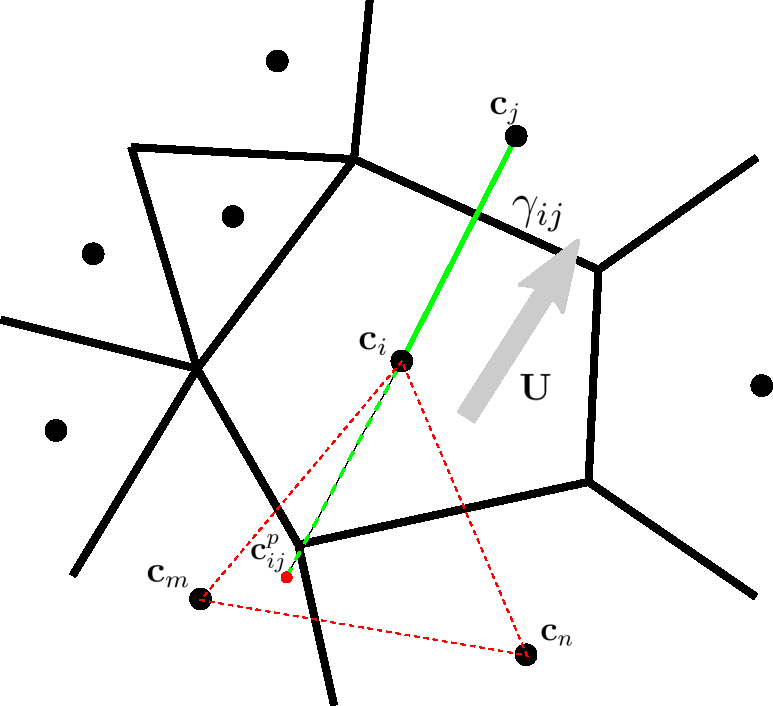
\includegraphics[width=0.4\linewidth]{fvm_tvd.pdf}
\caption{Вспомогательный узел $\vec c^p_{ij}$ на конечнообъёмной сетке}
\label{fig:fvm_tvd}
\end{figure}

Будем считать, что скорость переноса $U$ -- известная функция.
Тогда запишем значения потоков высокого и низкого порядка согласно \cref{eq:tvd_fhl}:
\begin{equation}
\label{eq:tvd_fhl_fvm}
\begin{aligned}
&f^L_{ij} = U_{ij} u_i                 &\text{-- схема против потока}\\
&f^H_{ij} = U_{ij} \frac{u_i + u_j}{2} &\text{-- симметричная схема}.
\end{aligned}
\end{equation}

Поток при этом запишется по аналогии с \cref{eq:tvd_f}:
\begin{equation}
\label{eq:tvd_f_fvm}
f_{ij} = f^L_{ij} + \Phi(r_{ij}) \left( f^H_{ij} - f^L_{ij} \right).
\end{equation}

В одномерном случае для записи соотношения наклонов $r_i$ \cref{eq:tvd_ri} использовались
три точки: текущий узел $i$, узел против потока $i-1$, и узел по потоку $i+1$.
Для случае неструктурированной сетки лишь две из этих трёх точек являются
узлами коллокации: текущий узел $i$ и узел по потоку $j$. Определим точку
против потока симметричным отражением: $\vec{c}^p_{ij} = 2\vec c_i - \vec c_j$ (см. рис.~\ref{fig:fvm_tvd}).
Значение функции в этой точке обозначим как $u^p_{ij}$.
Тогда соотношение наклонов запишется в виде

\begin{equation}
\label{eq:tvd_ri_fvm}
r_i = \frac{u_i - u_{ij}^p}{u_j - u_i}
\end{equation}

Точка $\vec c^p$ (в отличии от $x_{i-1}$ из одномерного случая)
не является точкой коллокации. То есть
значение $u^p$ нельзя достать из вектора столбца сеточной функции $u$.
Однако, это значение можно интерполировать
по значениям в ближайших точках коллокации.

\subsubsection{Прямая интерполяция противопоточного значения}
\label{sec:direct_interpolate_up}
Так, в двумерном случае для определения $u^p_{ij}$
необходимо найти три точки коллокации,
ближайшие к точке $\vec c^p_{ij}$ и не лежащие на одной прямой (или две точки коллокации, помимо $c_i$). На рис.~\ref{fig:fvm_tvd}
они помечены индексами $\vec c_m$, $\vec c_n$).
И далее в треуольнике, образованном этими тремя
точками ($\triangle_{imn}$) провести
интерполяцию
по формуле \cref{eq:simplex_interp_2d}.
Специально отметим, что точка $\vec c^p_{ij}$
не обязана содержаться внутри 
треугольника $\triangle_{imn}$.

\subsubsection{Интерполяция противопоточного значения через значение градиентов}
\label{sec:grad_inteprolate_up}.
Другой подход к определению $u^p_{ij}$ основан на записи симметричной конечной разности
по направлению $\vec c_{ij}$:
\begin{equation*}
\left.\dfr{u}{c_{ij}}\right|_i = \frac{u_j - u^p_{ij}}{2|\vec c_{ij}|} \qquad \hence
u_{ij}^p = u_j - 2 |\vec c_{ij}| \left. \dfr{u}{c_{ij}}\right|_i.
\end{equation*}
Производная по направлению $c_{ij}$ находится как проекция градиента:
\begin{equation*}
|\vec c_{ij}| \left.\dfr{u}{c_{ij}}\right|_i = \vec c_{ij} \cdot (\nabla u)_i.
\end{equation*}
Таким образом, задача интерполяции сводится к задаче определения градиента функции
$u$ в узлах коллокации.

\subsubsection{Определение градиентов в узлах коллокации. Метод наименьших квадратов}

Будем рассматривать узел $i$, имеющий $N_i$ соседних узлов $j$.
Для каждого $j$ можно записать линейное приближение
\begin{equation*}
u_j = u_i + |\vec c_{ij}| \dfr{u}{c_{ij}} = u_i + \vec c_{ij} \cdot \nabla u, \qquad j = \overline{0, N_i-1}.
\end{equation*}
Для двумерного случая можно записать:
\begin{equation*}
(\vec c_{ij})_x \, \dfr{u}{x} + (\vec c_{ij})_y \, \dfr{u}{y} = u_j - u_i, \qquad j = \overline{0, N_i - 1}.
\end{equation*}
Это выражение -- есть система линейных уравнений с двумя неизвестными $\dsfr{u}{x}$, $\dsfr{u}{y}$ 
и $N_i$ строками. Запишем её в матричном виде:
\begin{equation*}
\begin{array}{llll}
A y = f, &  \text{ где } & A_{j0} = (\vec c_{ij})_x & \quad A_{j1} = (\vec c_{ij})_y,\\
         &               & y_{0} = \dsfr{u}{x}      & \quad y_{1} = \dsfr{u}{y},\\
         &               & f_{j} = u_j - u_i &.
\end{array}
\end{equation*}
В двумерном случае размерность матрицы $A$ есть $[N_i, 2]$
(для трёхмерной задачи следуя аналогичным рассуждениям получим матрицу с размерностью $[N_i, 3]$).

При этом в двумерном случае у конечного элемента будет минимум три грани (или четыре в трёхмерном случае). То есть $N_i \geq 3$ 
и полученная система имеет неизвестных больше, чем количество уравнений.
Эта система в общем случае не имеет точного решения,
но можно найти такие $y$, при котором невязка будет минимальной.
Определим невязку как 
$$
r_i = \sum_{j=0}^{N_i}\left(A_{ij}y_j\right) - f_i, \qquad i=0, 1.
$$
и будем минимизировать её квадрат
$$
F = \sum_i r_i^2 \to \min
$$
Запишем условие экстремума как
$$
\dfr{F}{y_i} = 2 \sum_j r_j \dfr{r_j}{y_i} =
               2 \sum_j \left( \sum_k \left( A_{jk} y_k\right) - f_j \right)A_{ji} = 0, \qquad i=0,1.
$$
Отсюда получим систему уравнений
$$
\sum_j \left( A_{ji} \sum_k \left( A_{jk} y_k\right) \right) = \sum_j A_{ji}f_j = 0, \qquad i=0,1.
$$
Или, возвращаясь к матричной записи,
$$
A^{T} A y = A^{T}f.
$$
Полученная система имеет размерность $2\times2$ (или $3\times3$ в трёхмерном случае).
Значение компонент градиента в точке коллокации запишется как её прямое решение:
$$
y = \left(A^T A\right)^{-1} A^T f.
$$
Отметим, что матрица $A$ зависит только от геометрии сетки.
Поэтому в программной реализации матричное выражение $\left(A^T A\right)^{-1} A^T $ может быть расчитано 
один раз для каждого узла коллокации на этапе инициализации.
Тогда определение градиента в центрах ячеек на этапе решения задачи 
сведётся к сборке вектора $f$ и умножении его на это выражение.

\subsubsection{Реализация для явной схемы}
Для примера рассмотрим написание TVD-схемы
рассмотрим чисто явную схему для полудискретизованного уравнения \cref{eq:tvd_fvm_transport}:
\begin{equation}
\label{eq:tvd_fvm_explicit_transport}
\left| V_i \right|
\frac{\hat u - u}{\tau}
+ \sum_{j\in {\rm nei}(i)} {f_{ij} \left|\gamma_{ij}\right|}
= 0.
\end{equation}
Для того, чтобы избежать повторного вычисления потоков $f_{ij}$ и $f_{ji}$,
будем собирать эту схему в цикле по граням. Пусть через границу притока нет (то есть для граничные граней $f_{ij} = 0$.
Тогда останется только цикл по внутренним граням:
\begin{equation}
\label{eq:tvd_fvm_assem}
\begin{array}{ll}
\hat u = u                                               & \textrm{-- инициализируем следующий шаг}\\
\textbf{for } s \in\textrm{internal}                     & \textrm{-- цикл по внутренним граням}\\ 
\qquad i,j = \textrm{nei\_cells(s)}                      & \textrm{-- две ячейки, соседние с текущей гранью}\\
\qquad \vec U_{ij}                                       & \textrm{-- вектор скорости в центре грани}\\
\qquad \vec n_{ij}                                       & \textrm{-- вектор нормали к грани от ячейки i к j}\\
\qquad U_{ij} = \vec U_{ij} \cdot \vec n_{ij}            & \textrm{-- проекция скорости на нормаль}\\
\qquad \textbf{if } U_{ij} \leq 0                        & \textrm{-- схема против потока}\\
\qquad \qquad \textrm{swap}(i, j); U_{ij} = -U_{ij}      & \textrm{-- гарантируем, что жидкость течет от $i$ к $j$}\\
\qquad \textbf{endif}                                    & \textrm{}\\
\qquad f^L_{ij} = U_{ij} u_i                             & \textrm{-- поток 1-го порядка \cref{eq:tvd_fhl_fvm}}\\
\qquad f^H_{ij} = U_{ij} (u_i + u_j) / 2                 & \textrm{-- поток 2-го порядка \cref{eq:tvd_fhl_fvm}}\\
\qquad \vec c_i, \vec c_j                                & \textrm{-- центры ячеек}\\
\qquad \vec c^p = 2 \vec c_i - \vec c_j                  & \textrm{-- вспомогательная точка}\\
\qquad u^p = \textrm{interpolate}(i, j, u, \vec c^p)     & \textrm{-- интерполируем $u$ в точке $\vec c^p$}\\
\qquad r = \sfrac{(u_i - u^p)}{(u_j - u_i)}              & \textrm{-- отношение наклонов \cref{eq:tvd_ri_fvm}}\\
\qquad F = \textrm{limiter}(r)                           & \textrm{-- ограничитель \cref{eq:tvd_limiter}}\\
\qquad f_{ij} = f^L_{ij} + F (f^H_{ij} - f^L_{ij})       & \textrm{-- вычисление потока \cref{eq:tvd_f_fvm}}\\
\qquad \hat u_i\minuseq\tau/|V_i|\,f_{ij}\,|\gamma_{ij}| & \textrm{-- добавление в противопотоковую ячейку}\\
\qquad \hat u_j\pluseq \tau/|V_j|\,f_{ij}\,|\gamma_{ij}| & \textrm{-- добавление в попотоковую ячейку}\\
\textbf{endfor}                                          & \\
\end{array}
\end{equation}
Отметим, что использование
противоположенного знака при добавлении в правую
от грани ячейку $j$ связано с тожедством \cref{eq:tvd_fij_fji}.
То есть на самом деле в ячейку $j$
должен бы добавляться поток $f_{ji}$,
но поскольку отдельной обработки этого направления не предусмотрено,
мы добавляем $f_{ij}$ с обратным знаком.
При реализации функции $\textrm{interpolate}$ должен использоваться один из методов, изложенных
в пп.~\ref{sec:direct_interpolate_up}, \ref{sec:grad_inteprolate_up}.

\subsection{Задание для самостоятельной работы}
В тесте \ename{[transport2-fvm-upwind-explicit]}
из файла \ename{transport_fvm_solve_test.cpp}
реализовано решение
двумерного уравнения переноса 
по явной противопотоковой схеме.
Реализация алгоритма
в целом соответствует циклу \cref{eq:tvd_fvm_assem}
с упрощениями, следующими из отсутствия
необходимости вычислять $r$ в схеме против потока (где всегда $F=0$).

Отталкиваясь от этого теста нужно решить двумерное уравнение переноса
с помощью МКО аппроксимации на неструктурированной
сетке.  Использовать постановку из п.~\ref{sec:circle_transport} с $\sigma=0.1$.
Рассмотреть схему против потока и MC TVD-схему пространственной аппроксимации и явную схему для дискретизации по времени.
Для интерполяции противопотокового значения $u^p$ использовать
алгоритм \ref{sec:grad_inteprolate_up}. 

Неструктурированную сетку строить с помощью скрипта \ename{test_data/hexagrid.py}.
Количество элементов сетки подобрать так, чтобы видеть эффект от применения схемы высокого порядка.

\begin{enumerate}
\item
Проиллюстрировать динамику численного решения на неструктурированной конечнообъёмной сетке.
Сравнить решение MC и Upwind.
\item
Для выбранной сетки опытным путём определить максимально допустимый шаг по времени, при котором решение не разваливается;
\item 
Посчитать нормы отклоения полученного численного решения от известного точного (по максимуму и среднеквадратичную):
\begin{align*}
&n_{max} = 1 - \max\limits_{i} (u_i); \\
&n_2 = \left(\dfrac{\sum_i { \left(u_i - u^e(c_i)\right)^2 \left| V_i \right| }}{\sum_i \left| V_i \right|}\right)^{1/2}
\end{align*}
Нарисовать графики этих норм от времени $n(t)$ для двух рассмотренных схем. 
\end{enumerate}

\paragraph{Рекомендации к программированию}
Для вычисления градиентов в центрах ячеек
использовать класс \cvar{FvmCellGradient} из файла \ename{fvm/fvm_assembler.hpp}, экземпляр которого нужно создать на этапе инициализации задачи.
Тогда для вычисления градиентов от известной сеточной функции \cvar{u}
достаточно вызывать метод \cvar{FvmCellGradient::compute}.

\section{Лекция 16 (06.11)}

\subsection{Алгебраический подход к построению нелинейных TVD схем}
TODO

\subsection{Схемы с искусственной вязкостью}
TODO
\subsubsection{Направленная искусственная вязкость}
TODO
\subsubsection{SUPG}
TODO


\subsection{Задание для самостоятельной работы}
\label{sec:hw_supg}
В тестовом примере \cvar{[convdiff-fem-supg]} из файла \ename{convdiff_fem_test.cpp}
производится численного решение одномерного нестационарного уравнения конвекции-диффузии
$$
\dfr{u}{t} + v \dfr{u}{x} - \eps \dfrq{u}{x} = 0
$$
в области $x\in[0, 4]$
с точным решением вида
$$
u^e(x, t) = \frac{1}{\sqrt{4\pi \eps (t + t_0)}} \exp\left(-\frac{(x - v t)^2}{4\eps(t+t_0)}\right)
$$
Точное решение используется для формулировки начальных ($t=0$) и граничных ($x=0,4$) условий первого рода.
Результат расчёта сохраняется в файл \ename{convdiff-supg.vtk.series}.

Задача полудискретизуется по схеме Кранка-Николсон c шагом по времени, вычисленным через число Куранта $\rm C = 0.5$.

После дискретизации задача сводится к СЛАУ относительно неизвестного сеточного вектора $u$
$$
\begin{array}{ll}
\mat A u = \mat B \check u. \\
\mat A = \mat M + \tau\theta \mat K + \eps\tau\theta \mat S, \\
\mat B = \mat M - \tau(1-\theta)\mat K - \eps\tau(1-\theta) \mat S.
\end{array}
$$
Здесь матрица масс $\mat M$ -- результат коненчноэлементной аппроксимации единичного оператора,
матрица переноса $\mat K$ -- конвективного оператора,
а матрица жёсткости $\mat S$ -- оператора диффузии,
$\tau$ -- шаг по времени, и для схемы Кранка--Николсон $\theta=0.5$.


Стабилизированные матрицы вычислялись по следующим формулам:
\begin{equation*}
\begin{WithArrows}
\mat M =& \int\limits_\Omega \phi_j (\phi_i + s \vec v \cdot \nabla \phi_i) \, d\vec x
           \\[10pt]
\mat K =& \arint{\vec v \cdot \nabla \phi_j (\phi_i + s \vec v \cdot \nabla \phi_i)}{\Omega}{\vec x}
           \\[10pt]
\mat S =& -\arint{\nabla^2 \phi_j (\phi_i + s\vec v \cdot \nabla \phi_i)}{\Omega}{\vec x}
           \Arrow{по формуле \cref{eq:partint_laplace_fg}}\\[10pt]
       =& \arint{\nabla \phi_j \cdot \nabla(\phi_i + s\vec v \cdot \nabla \phi_i)}{\Omega}{\vec x}
           \Arrow{если $\phi_i$ линейны, то $\nabla^2\phi_i = 0$}\\[10pt]
       =& \arint{\nabla \phi_j \cdot \nabla\phi_i}{\Omega}{\vec x}
\end{WithArrows}
\end{equation*}
где $s = \mu h / \left | v \right|^2$, $h$ -- характерный линейный размер элемента, а $\mu$ -- параметр SUPG-стабилизации.

Сборки необходимых матриц осуществляется в процедуре \cvar{asseble_solver}.
Локальные матрицы для операторов $\mat M$, $\mat K$ вычисляются с помощью численного интегрирования в процедуре
\cvar{custom_matrix}, которой в качестве аргумента передаётся функция подинтегрального выражения.

Необходимо:
\begin{enumerate}
\item В одномерном тесте \cvar{[convdiff-supg]} с помощью анимированных графиков продемонстрировать наличие осцилляций
      при выбранных параметрах решения при отсутствии стабилизации \cvar{mu_supg = 0}, а так же эффект от SUPG-слагаемого (\cvar{mu_supg > 0});
\item Нарисовать в сравнении результаты расчёта на конечный промежуток времени для различных $\mu$;
\item Подобрать оптимальную величину параметра $\mu$, минимизирующую норму отклонения численного решения от точного;
\item Написать аналогичный тест для двумерного случая (решение в единичном квадрате) c точным решением
$$
u^e(x, t) = \frac{1}{4\pi \eps (t + t_0)} \exp\left(-\frac{(x - v_x t)^2 + (y - v_y t)^2}{4\eps(t+t_0)}\right)
$$
Использовать $\vec v  = (1, 1)$. Взять треугольную сетку, построенную процедурой \ename{trigrid.py}. Проанализировать результаты, полученные на грубой и подробной сетке.
\end{enumerate}

В целом имеющийся решатель не зависит от геометрической размерности задачи.
Для двумерного решателя нужно
\begin{itemize}
\item изменить значение точного решения и скорости (функции \cvar{velocity}, \cvar{nonstat_solution});
\item внести изменения в процедуру постановки граничных условий в функциях \cvar{assemble_solver}, \cvar{assemble_rhs} (сместо двух точек начала и конца одномерной области
необходимо пройтись по всем граничным узлам двумерной сетки);
\end{itemize}

\section{Лекция 17 (23.11)}

\subsection{Моделирирование течения вязкой несжимаемой жикости методом конечных разностей}
\subsubsection{Система уравнений Навье-Стокса}

Будем рассматривать стационарную двумерную систему уравнений
Навье-Стокса для вязкой несжимаемой жидкости.
В безразмерном консервативном виде в декартовой системе координат она имеет вид

\begin{align}
    \label{eq:ns2d_u}
    & \dfr{u^2}{x} + \dfr{uv}{y} =
        -\dfr{p}{x}
        + \frac{1}{\Ren}\left(\dfrq{u}{x} + \dfrq{u}{y}\right),\\[5pt]
    \label{eq:ns2d_v}
    & \dfr{uv}{x} + \dfr{v^2}{y} =
        -\dfr{p}{y}
        + \frac{1}{\Ren}\left(\dfrq{v}{x} + \dfrq{v}{y}\right), \\[5pt]
    \label{eq:ns2d_div}
    &\dfr{u}{x} + \dfr{v}{y} = 0.
\end{align}

Неизвестными являются поля скорости: $u$ -- в направлении оси $x$,
$v$ -- в направлении оси $y$, и давления $p$.

Число Рейнольдса определено через характерную скорость $U$, [м/c] и
характерный линейный размер $L$, [м] как
\begin{equation*}
    \Ren = \frac{UL\rho}{\mu},
\end{equation*}
где $\rho$, [кг/м$^3$] -- постоянная (вследствии несжимаемости) плотность жидкости, а
$\mu$, [Па$\cdot$с] -- динамическая вязкость жидоксти.

Характерое значение для давление выпишется в виде:
$ p^0 = \rho U^2 $, [Па].

Для решения этой системы будем использовать метод конечных разностей
с аппроксимацией по пространству второго порядка и последовательное (раздельное) решение входящих в неё
уравнений.

Глядя на вид уранений \cref{eq:ns2d_u,eq:ns2d_v,eq:ns2d_div}
можно выделить несколько проблем, которые необходимо решить
при построении расчётной схемы:
\begin{itemize}
\item нелинейность конвективного оператора в \eqref{eq:ns2d_u}, \eqref{eq:ns2d_v},
\item отсутствие явного уравнения для определения давления,
\item аппркосимация первых производных для давления и скорости со вторым порядком точности.
\end{itemize}


Для решения первой проблемы будем использовать итерационный процесс с линеаризацией -- то есть
записывать уравнение на итерационном слое используя значения неизвестных полей с прошлого слоя.
Вторую проблему будем решать с помощью алгоритма SIMPLE
связывания давления и скорости (Pressure-Velocity Coupling).
Решать третью проблему будем с помощью пространственной аппроксимации на разнесённой сетке (Staggered Grid).

\subsubsection{Схема расчёта}

Стационарную задачу \eqref{eq:ns2d_u}-\eqref{eq:ns2d_div} будем решать
методом установления. Для этого в первые два уравнения введём фиктивную
производную по времени, которую распишем по неявной двухслойной схеме с шагом $\tau$.
Тогда задача на одном итерационном слое примет вид

\begin{align}
    \label{eq:ns2d_semi_u}
    & \frac{\hat u - u}{\tau} + \dfr{u \hat u}{x} + \dfr{v \hat u}{y} =
        -\dfr{\hat p}{x}
        + \frac{1}{\Ren}\left(\dfrq{\hat u}{x} + \dfrq{\hat u}{y}\right),\\[5pt]
    \label{eq:ns2d_semi_v}
    & \frac{\hat v - v}{\tau} + \dfr{u\hat v}{x} + \dfr{v \hat v}{y} =
        -\dfr{\hat p}{y}
        + \frac{1}{\Ren}\left(\dfrq{\hat v}{x} + \dfrq{\hat v}{y}\right), \\[5pt]
    \label{eq:ns2d_semi_div}
    &\dfr{\hat u}{x} + \dfr{\hat v}{y} = 0.
\end{align}

При записи была произведена линеаризация конвективного слагаемого:
один из множителей в производной был отнесён на предыдущий
временной слой. В остальном схема неявная.

На временном слое значения $u, v, p$
известны, а $\hat u, \hat v, \hat p$ подлежат определению.

Критерием выхода из итерационного процесса является пороговое условие на невязку,
вычисленную с использованием найденных на слое значений неизвестных:
\begin{align}
    \nonumber
    &r_u = \dfr{\hat u \hat u}{x} + \dfr{\hat u \hat v}{y}
        + \dfr{\hat p}{x}
        - \frac{1}{\Ren}\left(\dfrq{\hat u}{x} + \dfrq{\hat u}{y}\right),\\[5pt]
    \nonumber
    &r_v = \dfr{\hat u\hat v}{x} + \dfr{\hat v \hat v}{y}
        +\dfr{\hat p}{y}
        - \frac{1}{\Ren}\left(\dfrq{\hat v}{x} + \dfrq{\hat v}{y}\right), \\[5pt]
    \label{eq:ns2d_residual}
    &\max(\lVert r_u \rVert, \lVert r_v \rVert) < \eps.
\end{align}

\subsubsubsection{Метод SIMPLE}
\label{sec:simple-algo}

Приведём алгоритм для явного выражения уравнения для давления из
уравнения неразрывности \eqref{eq:ns2d_semi_div}.

Распишем искомые перенные в виде суммы 
\begin{equation}
    \label{eq:ns2d_decomp}
\begin{array}{l}
    \hat u = u^* + u',\\
    \hat v = v^* + v',\\
    \hat p = p + p'.
\end{array}
\end{equation}

Пусть введённые выше поля $u^*$, $v^*$ удовлетворяют уравнениям
\begin{align}
    \label{eq:ns2d_ustar}
    &u^* + \tau\dfr{u u^*}{x} + \tau\dfr{v u^*}{y}
       - \frac{\tau}{\Ren}\left(\dfrq{u^*}{x} + \dfrq{u^*}{y}\right)
       = -\tau\dfr{p}{x} + u, \\[5pt]
    \label{eq:ns2d_vstar}
    &v^* + \tau\dfr{u v^*}{x} + \tau\dfr{v v^*}{y}
       - \frac{\tau}{\Ren}\left(\dfrq{v^*}{x} + \dfrq{v^*}{y}\right)
       = -\tau\dfr{p}{y} + v.
\end{align}

Тогда уравнение для поправки $u'$ запишем вычтя последнее выражение из
уравнения \eqref{eq:ns2d_semi_u}, умноженного на $\tau$:

\begin{equation}
    \label{eq:ns2d_uprime}
    u' + \tau\dfr{u u'}{x} + \tau\dfr{v u'}{y}
       - \frac{\tau}{\Ren}\left(\dfrq{u'}{x} + \dfrq{\hat u'}{y}\right)
       = -\tau\dfr{p'}{x}.
\end{equation}

Основная идея алгоритма SIMPLE заключается в приближённом представлении выражения \eqref{eq:ns2d_uprime}
в явном виде относительно поправки. Для этого все дифференциальные операторы, включающие в себя поправку скорости,
из выражения убираются, а для компенсации в правую часть добавляется множитель $d^u$:

\begin{equation}
    \label{eq:ns2d_uprime_approx}
    u' \approx -\tau d^u(x, y) \dfr{p'}{x}.
\end{equation}

Аналогичные рассуждения в отношении поправки поперечной скорости $v'$ приводят к выражению

\begin{equation}
    \label{eq:ns2d_vprime_approx}
    v' \approx -\tau d^v(x, y) \dfr{p'}{y}.
\end{equation}

К точному определению значения полей $d^u$, $d^v$ вернёмся позднее, когда будем расписывать
эти выражения на матричном уровне.

Далее используем уравнение неразрывности \cref{eq:ns2d_semi_div}. Подставим
в него разложения \cref{eq:ns2d_decomp} и используем
\cref{eq:ns2d_uprime_approx,eq:ns2d_vprime_approx}.
Тогда
получим уравнение Пуассона с непостоянным по пространству векторным коэффициентом диффузии $\left(d^u, d^v\right)$
относительно поправки давления $p'$:
\begin{equation}
    \label{eq:ns2d_pprime_diff}
    -\left[
    \dfr{}{x}\left(
       d^u \dfr{p'}{x} 
            \right)
    +\dfr{}{y}\left(
       d^v \dfr{p'}{y} 
            \right)
    \right]
    =
    -\frac{1}{\tau}\left(
            \dfr{u^*}{x} + \dfr{v^*}{y}
    \right).
\end{equation}

Определим порядок вычислений на итерационном слое.
Напомним, что значения $u, v, p$ с
предыдущего слоя нам известно и задача
состоит в нахождении значений $\hat u, \hat v, \hat p$
на текущем слое.

\begin{enumerate}
\item Из уравнений \eqref{eq:ns2d_ustar}, \eqref{eq:ns2d_vstar}
      вычисляются значения $u^*, v^*$;
\item Они используются для вычисления правой части уравнения \eqref{eq:ns2d_pprime_diff},
      в результате решения которого находится поправка давления $p'$;
\item Дифференцируя найденную поправку давления найдём поправки скорости $u', v'$
      из выражений \eqref{eq:ns2d_uprime_approx}, \eqref{eq:ns2d_vprime_approx};
\item Окончательно выразим значения переменных для текущего слоя из \eqref{eq:ns2d_decomp}.
      Для улучшения стабильности алгоритма значение давления вычисляют
      с некоторым коэффициентом релаксации $\alpha_p$:
      \begin{equation*}
           \hat p = p + \alpha_p p';
      \end{equation*}
\item Далее проводится вычисление невязки с ипользованием найденных значений $\hat u, \hat v, \hat p$
      из выражения \eqref{eq:ns2d_residual}. Если она недостаточно мала,
      то выполняется присваивание
      $
           u = \hat u, \; v=\hat v, \; p = \hat p
      $ 
      и возвращение на шаг 1.
\end{enumerate}

Полученные на каждом шаге итерационного процесса компоненты скорости $\hat u, \hat v$
точно удовлетворяют уравнению неразрывности \eqref{eq:ns2d_semi_div} в ``чёрных'' узлах сетки, но
уравнения движения \eqref{eq:ns2d_semi_u}, \eqref{eq:ns2d_semi_v} выполняются лишь приближённо.

Всего в алгоритме SIMPLE есть два параметра: коэффициент
релаксации давления $\alpha_p$ и фиктивный шаг по времени $\tau$ (который можно трактовать как коэффициент релаксации скорости).

\subsubsection{Пространственная аппроксимация}

Для численной реализации алгоритма решения
необходимо провести пространственную аппроксимацию полудискретизованных
выражений
\eqref{eq:ns2d_ustar}, \eqref{eq:ns2d_vstar}, \eqref{eq:ns2d_uprime_approx},
\eqref{eq:ns2d_vprime_approx}, \eqref{eq:ns2d_pprime_diff}.

\subsubsubsection{Разнесённая сетка}

Будем использовать структурированную четырёхугольную сетку
с постоянным шагом по пространству.
При этом неизвестные параметры будем задавать
по схеме, представленной на \figref{fig:staggered_grid}.

\begin{figure}[h]
\centering
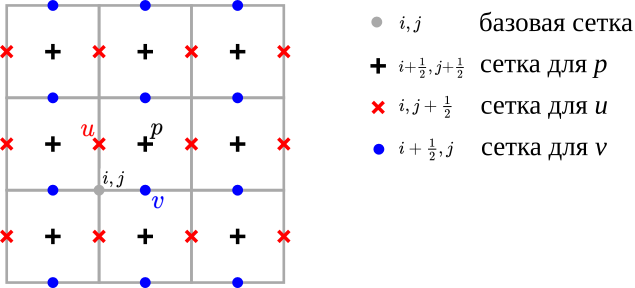
\includegraphics[width=0.6\linewidth]{staggered_grid.png}
\caption{Разнесённая сетка}
\label{fig:staggered_grid}
\end{figure}

Введём разбиение сетки:
$n_x$ -- количество ячеек в направлении $x$,
$n_y$ -- количество ячеек в направлении $y$.

Очевидно, что при использовании такого разнесённого шаблона,
количество точек, в которых заданы значения, будет
различным для разных параметров.
Так количество узловых значений давления будет равно $n_x \times n_y$,
продольной скорости $u$ -- $(n_x+1) \times n_y$, а поперечной $v$ -- $n_x \times (n_y+1)$.

Использование такого расположения узловых точек
даёт преимущество при аппроксимации
первых производных. Так, конечная разность
\begin{equation*}
\left.\dfr{p}{x}\right|_{i, j+\tfrac12} = \frac{p_{i+\tfrac12,j+\tfrac12} - p_{i-\tfrac12,j+\tfrac12}}{h_x} + o(h_x^2)
\end{equation*}
будем симметричной в узле $i,j+\tfrac12$, где задана
компонента скорости $u$, и поэтому будет иметь там второй порядок точности.

Выражения \eqref{eq:ns2d_ustar}, \eqref{eq:ns2d_uprime_approx} аппроксимируются
на сетке для $u$, выражения \eqref{eq:ns2d_vstar}, \eqref{eq:ns2d_vprime_approx} -- 
на сетке для $v$, а \eqref{eq:ns2d_pprime_diff} -- на сетке для $p$.

Введём сквозную линейную нумерацию узлов сетки: нулевой узел разположим в левом нижнем углу,
далее будем индексировать слева направа и потом снизу вверх.
Для основной сетки перевод двумерного индекса $i,j$ в сквозной индекс будет проводится по формуле
\begin{equation}
    \label{eq:ns2d_kij}
    k(i,j) = j(n_x+1)+i.
\end{equation}
Для сеток, на которых заданы сеточные параметры, такой перевод примет вид
\begin{align}
    \label{eq:ns2d_kipjp}
    &k(i+\tfrac12,j+\tfrac12) = jn_x + i, \quad - \; \text{сетка для давления } p\\[10pt]
    \label{eq:ns2d_kijp}
    &k(i,j+\tfrac12) = j(n_x+1) + i, \quad - \;  \text{сетка для продольной скорости } {\color{red} u} \\[10pt]
    \label{eq:ns2d_kipj}
    &k(i+\tfrac12,j) = jn_x + i, \quad - \; \text{сетка для поперечной скорости } {\color{blue} v}
\end{align}

\subsubsubsection{Уравнения движения}

Запишем конечноразностную аппроксимацию уравнения \eqref{eq:ns2d_ustar} для пробной скорости $u^*$ в ``красных'' узлах сетки
$\left(i, j+\tfrac12\right)$:

\begin{align}
    \label{eq:ns2d_ustar_discr}
    u^*_{i, j+\tfrac12} 
        &+ \frac{\tau}{h_x}
          \left(
            \left(u u^*\right)_{i+\tfrac12,j+\tfrac12}-
            \left(u u^*\right)_{i-\tfrac12,j+\tfrac12}
          \right)  \\[10pt]
    \nonumber
        &+ \frac{\tau}{h_y}
          \left(
            \left(v u^*\right)_{i,j+1}-
            \left(v u^*\right)_{i,j}
          \right)   \\[10pt]
    \nonumber
       &-\frac{1}{\Ren}\frac{\tau}{h_x^2}
          \left(
            u^*_{i-1,j+\tfrac12} - 2 u^*_{i,j+\tfrac12} + u^*_{i+1,j+\tfrac12}
          \right)   \\[10pt]
    \nonumber
       &-\frac{1}{\Ren}\frac{\tau}{h_y^2}
          \left(
            u^*_{i,j-\tfrac12} - 2 u^*_{i,j+\tfrac12} + u^*_{i,j+\tfrac32}
          \right)   \\[10pt]
    \nonumber
       &= u_{i,j+\tfrac12} -\frac{\tau}{h_x}\left(p_{i+\tfrac12,j+\tfrac12} - p_{i-\tfrac12,j+\tfrac12}\right).
\end{align}

В приведённом выражении
за исключением конвективных слагаемых вида $u u$ все остальные
сеточные вектора используются на своих сетках.
Конвективные слагаемые распишем через полусуммы вида:
\begin{equation*}
    u_{i+\tfrac12} = \frac{u_{i} + u_{i+1}}{2} + o(h^2)
\end{equation*}

Тогда
\begin{align*}
    \left(u u^*\right)_{i+\tfrac12,j+\tfrac12} =&
        \left(u_{i+\tfrac12,j+\tfrac12} \vphantom{u^*_{\tfrac12}}\right)\left(u^*_{i+\tfrac12,j+\tfrac12}\right) =
        \frac14 \left(u_{i, j+\tfrac12} + u_{i+1,j+\tfrac12}\vphantom{u^*_{\tfrac12}}\right)
                \left(u^*_{i, j+\tfrac12} + u^*_{i+1,j+\tfrac12}\right), \\[10pt]
    \left(u u^*\right)_{i-\tfrac12,j+\tfrac12} =&
        \frac14 \left(u_{i, j+\tfrac12} + u_{i-1,j+\tfrac12}\vphantom{u^*_{\tfrac12}}\right)
                \left(u^*_{i, j+\tfrac12} + u^*_{i-1,j+\tfrac12}\right), \\[10pt]
    \left(v u^*\right)_{i,j+1} =&
        \frac14 \left(v_{i+\tfrac12, j+1} + v_{i-\tfrac12,j+1}\vphantom{u^*_{\tfrac12}}\right)
                \left(u^*_{i, j+\tfrac32} + u^*_{i,j+\tfrac12}\right), \\[10pt]
    \left(v u^*\right)_{i,j} =&
        \frac14 \left(v_{i+\tfrac12, j} + v_{i-\tfrac12,j}\vphantom{u^*_{\tfrac12}}\right)
                \left(u^*_{i, j+\tfrac12} + u^*_{i,j-\tfrac12}\right).
\end{align*}

Схему \eqref{eq:ns2d_ustar_discr} можно записать в виде системы линейных уравнений вида
\begin{equation}
    \label{eq:ns2d_ustar_slae}
    S^u u^* = b^{u}.
\end{equation}
Сеточная матрица $A^u$ будет иметь $(n_x+1)n_y$ строк.
Для строки, соответствующей $\left(i,j+\tfrac12\right)$ узлу ненулевыми будут столбцы,
соответствующие узлам:
\begin{itemize}
\item $\left(i,j+\tfrac12\right)$,
\item $\left(i+1,j+\tfrac12\right)$,
\item $\left(i-1,j+\tfrac12\right)$,
\item $\left(i,j+\tfrac32\right)$,
\item $\left(i,j-\tfrac12\right)$.
\end{itemize}

В случае использования стандартной нумерации узлов структурированной сетки,
когда нулевой индекс соответствуют левому нижнему узлу и далее нумерация идёт
с быстрым индексом $i$, то матрица будет пятидиагональной.


Подставим полученные выражения в конвективную часть выражения \eqref{eq:ns2d_ustar_discr}.
Множитель при диагональном элементе $u^*_{i,j+\tfrac12}$ будет равен:
\begin{align*}
        \frac{\tau}{4}\Biggl(
         \underbrace{\frac{u_{i,j+\tfrac12} - u_{i-1,j+\tfrac12}}{h_x}}_{\left.\ddfr{u}{x}\right|_{i-\tfrac12,j+\tfrac12}}
        +\underbrace{\frac{u_{i+1,j+\tfrac12} - u_{i,j+\tfrac12}}{h_x}}_{\left.\ddfr{u}{x}\right|_{i+\tfrac12,j+\tfrac12}}
        +\underbrace{\frac{v_{i+\tfrac12,j+1} - v_{i+\tfrac12,j}}{h_y}}_{\left.\ddfr{v}{y}\right|_{i+\tfrac12,j+\tfrac12}}
        +\underbrace{\frac{v_{i-\tfrac12,j+1} - v_{i-\tfrac12,j}}{h_y}}_{\left.\ddfr{v}{y}\right|_{i-\tfrac12,j+\tfrac12}}
        \Biggr)
\end{align*}

Сумма первого и четвёртого слагаемых представляет собой разностный
аналог уравнения неразрывности \eqref{eq:ns2d_semi_div}, записанной для ``чёрного'' узла
сетки $i-\tfrac12, j+\tfrac12$ относительно компонент
скорости с предыдущей итерации.
Как было сказано ранее,
в настоящем алгоритме
уравнение неразрывности для итоговых по результатам итерации скорости в этих узлах выполняется точно.
Поэтому эта сумма в точности будет равна нулю. Аналогичный результат получится
и для суммы второго и третьего слагаемых. Отсюда следует вывод, что
конвективное слагаемое не даёт вклад в диагональ итоговой матрицы (как и следовало ожидать от симметричной аппроксимации).

Окончательно запишем все пять ненулевых вхождений в строку матрицы:
\begin{align}
    \label{eq:ns2d_au}
    S^u\left[
        k\left(i,j+\tfrac12\right),
        k\left(i,j+\tfrac12\right)\right]
        &= 1 + \frac{2\tau}{\Ren}\left(\frac{1}{h_x^2} + \frac{1}{h_y^2}\right)
        \quad - \;\text{основная диагональ}, \\[10pt]
    \nonumber
    S^u\left[
        k\left(i,j+\tfrac12\right),
        k\left(i+1,j+\tfrac12\right)\right]
        &= -\frac{\tau}{\Ren}\frac{1}{h_x^2}
           +\frac{\tau}{4h_x}\left(u_{i,j+\tfrac12}+u_{i+1,j+\tfrac12}\right)
        \quad - \;\text{первая верхняя диагональ}, \\[10pt]
    \nonumber
    S^u\left[
        k\left(i,j+\tfrac12\right),
        k\left(i-1,j+\tfrac12\right)\right]
        &= -\frac{\tau}{\Ren}\frac{1}{h_x^2}
           -\frac{\tau}{4h_x}\left(u_{i,j+\tfrac12}+u_{i-1,j+\tfrac12}\right)
        \quad - \;\text{первая нижняя диагональ}, \\[10pt]
    \nonumber
    S^u\left[
        k\left(i,j+\tfrac12\right),
        k\left(i,j+\tfrac32\right)\right]
        &= -\frac{\tau}{\Ren}\frac{1}{h_y^2}
           +\frac{\tau}{4h_y}\left(v_{i+\tfrac12,j+1}+v_{i-\tfrac12,j+1}\right)
        \quad - \;\text{вторая верхняя диагональ}, \\[10pt]
    \nonumber
    S^u\left[
        k\left(i,j+\tfrac12\right),
        k\left(i,j-\tfrac12\right)\right]
        &= -\frac{\tau}{\Ren}\frac{1}{h_y^2}
           -\frac{\tau}{4h_y}\left(v_{i+\tfrac12,j}+v_{i-\tfrac12,j}\right)
        \quad - \;\text{вторая нижняя диагональ}.
\end{align}
Здесь $k(i,j)$ -- функция перевода двумерного индекса в сквозной \eqref{eq:ns2d_kijp}.

Аналогичные выкладки для второго из уравнений движения \eqref{eq:ns2d_vstar}
дают систему уравнений
\begin{equation}
    \label{eq:ns2d_vstar_slae}
    S^v v^* = b^{v},
\end{equation}
элементы пятидиагональной матрицы которой имеют вид
\begin{align}
    \label{eq:ns2d_av}
    S^v\left[
        k\left(i+\tfrac12,j\right),
        k\left(i+\tfrac12,j\right)\right]
        &= 1 + \frac{2\tau}{\Ren}\left(\frac{1}{h_x^2} + \frac{1}{h_y^2}\right)
        \quad - \;\text{основная диагональ}, \\[10pt]
    \nonumber
    S^v\left[
        k\left(i+\tfrac12,j\right),
        k\left(i+\tfrac32,j\right)\right]
        &= -\frac{\tau}{\Ren}\frac{1}{h_x^2}
           +\frac{\tau}{4h_x}\left(u_{i+1,j+\tfrac12}+u_{i+1,j-\tfrac12}\right)
        \quad - \;\text{первая верхняя диагональ}, \\[10pt]
    \nonumber
    S^v\left[
        k\left(i+\tfrac12,j\right),
        k\left(i-\tfrac12,j\right)\right]
        &= -\frac{\tau}{\Ren}\frac{1}{h_x^2}
           -\frac{\tau}{4h_x}\left(u_{i,j+\tfrac12}+u_{i,j-\tfrac12}\right)
        \quad - \;\text{первая нижняя диагональ}, \\[10pt]
    \nonumber
    S^v\left[
        k\left(i+\tfrac12,j\right),
        k\left(i+\tfrac12,j+1\right)\right]
        &= -\frac{\tau}{\Ren}\frac{1}{h_y^2}
           +\frac{\tau}{4h_y}\left(v_{i+\tfrac12,j}+v_{i+\tfrac12,j+1}\right)
        \quad - \;\text{вторая верхняя диагональ}, \\[10pt]
    \nonumber
    S^v\left[
        k\left(i+\tfrac12,j\right),
        k\left(i+\tfrac12,j-1\right)\right]
        &= -\frac{\tau}{\Ren}\frac{1}{h_y^2}
           -\frac{\tau}{4h_y}\left(v_{i+\tfrac12,j}+v_{i+\tfrac12,j-1}\right)
        \quad - \;\text{вторая нижняя диагональ}.
\end{align}
Правая часть аппроксимируется в виде
\begin{equation*}
    b^{v^*}[k(i+\tfrac12, j)] = 1 - \frac{\tau}{h_y}\left(p_{i+\tfrac12, j+1} - p_{i+\tfrac12,j}\right).
\end{equation*}
Используется функция перевода двумерного индекса в сквозной из \eqref{eq:ns2d_kipj}.

\subsubsubsection{Уравнение для поправки давления}
Распишем уравнение \eqref{eq:ns2d_pprime_diff}
на ``чёрной'' сетке методом конечных разностей.
Для первого слагаемого получим
\begin{equation}
\label{eq:ns2d_d2pdx2}
\begin{array}{ll}
\left.\ddfr{}{x}\left(d^u \ddfr{p'}{x}\right) \right|_{i+\tfrac12, j+\tfrac12}
    &\approx
        \dfrac{1}{h_x}\left(
            d^u_{i+1, j+\tfrac12} \left. \ddfr{p'}{x} \right|_{i+1, j+\tfrac12} -
            d^u_{i, j+\tfrac12} \left. \ddfr{p'}{x} \right|_{i, j+\tfrac12}
        \right) \\[10pt]

    &=
        \dfrac{1}{h_x}\left(
            d^u_{i+1, j+\tfrac12} \dfrac{p'_{i+\tfrac32,j+\tfrac12} - p'_{i+\tfrac12,j+\tfrac12}}{h_x} - 
            d^u_{i, j+\tfrac12}  \dfrac{p'_{i+\tfrac12,j+\tfrac12} - p'_{i-\tfrac12,j+\tfrac12}}{h_x}
        \right).
\end{array}
\end{equation}
Аналогично расписываются остальные слагаемые. В результате получим систему линейных уравнений вида
\begin{equation}
    \label{eq:ns2d_pprime_slae}
    A^p p' = b^p,
\end{equation}
где ненулевые коэффициенты пятидиагональной матрицы примут вид
\begin{align}
    \label{eq:ns2d_ap}
    A^p[k(i+\tfrac12, j+\tfrac12), k(i+\tfrac12, j+\tfrac12)] =&
        \frac{1}{h_x^2}\left( d^u_{i+1,j+\tfrac12} + d^u_{i,j+\tfrac12} \right)
        +\frac{1}{h_y^2}\left( d^v_{i+\tfrac12,j} + d^v_{i+\tfrac12,j+1} \right), \\[10pt]
    \nonumber
    A^p[k(i+\tfrac12, j+\tfrac12), k(i+\tfrac32, j+\tfrac12)] =&
        -\frac{1}{h_x^2}d^u_{i+1,j+\tfrac12}, \\[10pt]
    \nonumber
    A^p[k(i+\tfrac12, j+\tfrac12), k(i-\tfrac12, j+\tfrac12)] =&
        -\frac{1}{h_x^2}d^u_{i,j+\tfrac12}, \\[10pt]
    \nonumber
    A^p[k(i+\tfrac12, j+\tfrac12), k(i+\tfrac12, j+\tfrac32)] =&
        -\frac{1}{h_y^2}d^v_{i+\tfrac12,j+1}, \\[10pt]
    \nonumber
    A^p[k(i+\tfrac12, j+\tfrac12), k(i+\tfrac12, j-\tfrac12)] =&
        -\frac{1}{h_y^2}d^v_{i+\tfrac12,j}.\\[10pt]
\end{align}
Столбец свободных членов аппроксимируется в виде
\begin{equation}
    \label{eq:ns2d_bp}
    b^p[k(i+\tfrac12,j+\tfrac12)] = 
        -\frac{1}{\tau}
        \left(
              \frac{u^*_{i+1,j+\tfrac12} - u^*_{i,j+\tfrac12}}{h_x}
            + \frac{v^*_{i+\tfrac12,j+1} - v^*_{i+\tfrac12,j}}{h_y}
        \right).
\end{equation}
Здесь используется функция перевода двумерного индекса в сквозной из $\eqref{eq:ns2d_kipjp}$.

Далее определим значения $d^u, d^v$.
Согласно идее алгоритма SIMPLE $d^u$ должна
быть такой функцией, которая максимально приближает
выражение \eqref{eq:ns2d_uprime} к \eqref{eq:ns2d_uprime_approx}.

Пространственная аппроксимация выражения \eqref{eq:ns2d_uprime}
приводит к системе уравнений
\begin{equation*}
    S^u u' = -\tau\dfr{p'}{x}
\end{equation*}
где матрица $S^u$ -- та же самая матрица, которая использовалась
при аппроксимации уравнения движения \eqref{eq:ns2d_ustar_discr}.

Сравнивая предыдущее выражение с \eqref{eq:ns2d_uprime_approx}
сделаем вывод, что $d^u$ должна быть такой, чтобы
\begin{equation*}
    d^u \dfr{p'}{x} \approx \left(S^u\right)^{\sminus 1} \dfr{p'}{x}.
\end{equation*}
То есть поэлементное умножение сеточного вектора ${d^u}$ 
на другой вектор
должно действовать похоже на умножение обратной к $S^u$ матрицы на этот же самый вектор.

Исходя из свойств матрицы $S^u$ \eqref{eq:ns2d_au} можно
положить 
\begin{equation}
    \label{eq:ns2d_du}
    d^u = \left({\rm diag}\left(S^u\right)\right)^{\sminus 1} = 
        \left(1 + \frac{2\tau}{\Ren}\left(\frac{1}{h_x^2} + \frac{1}{h_y^2}\right)\right)^{\sminus 1}
\end{equation}
и аналогично из \eqref{eq:ns2d_av}
\begin{equation}
    \label{eq:ns2d_dv}
    d^v = \left({\rm diag}\left(S^v\right) \right)^{\sminus 1}= 
        \left(1 + \frac{2\tau}{\Ren}\left(\frac{1}{h_x^2} + \frac{1}{h_y^2}\right)\right)^{\sminus 1}.
\end{equation}
Равентство коэффициентов $d^u = d^v$ -- следствие использования симметричной
аппроксимации конвективного слагаемого в уравнениях движения.

Таким образом мы получили выражения для коэффициентов уравнения для поправки давления,
которые зависят только от разбиения сетки.
В случае, если разбиение равномерное ($h_x = {\rm const}, h_y = {\rm const}$),
то все значения коэффициентов одинаковы.
Однако, для неравномерных разбиений, они будут зависеть
от пространства и задаваться на ``красной'' (для $d^u$) и ``синей'' (для $d^v$)
сетках.

В результате использования \eqref{eq:ns2d_du}, \eqref{eq:ns2d_dv} левая часть системы уравнений \eqref{eq:ns2d_pprime_slae}
будет постоянна на всех итерациях, что удобно для инициализации алгебраических решателей этой системы
(можно провести инициализацию один раз до начала счёта).

Это отличает эту систему от двух других систем, возникающих
из аппроксимации уравнений движения \eqref{eq:ns2d_ustar_slae}, \eqref{eq:ns2d_vstar_slae},
левые части которых зависят от значений с предыдущих
итерационных слоёв. Этот момент обуславливает выбор
решателей для этих систем, которые в эффективных гидродинамических кодах обычно
отличаются, от решателя для системы \eqref{eq:ns2d_pprime_slae}.


\subsubsubsection{Уравнение для поправки скорости}
И наконец рассмотрим аппроксимацию выражений \eqref{eq:ns2d_uprime_approx},
\eqref{eq:ns2d_vprime_approx}, которые примут явный вид
\begin{align}
    \label{eq:ns2d_uprime_discr}
    u'_{i,j+\tfrac12} = -\tau d^u_{i,j+\tfrac12} \frac{p'_{i+\tfrac12,j+\tfrac12} - p'_{i-\tfrac12, j+\tfrac12}}{h_x}, \\[10pt]
    \label{eq:ns2d_vprime_discr}
    v'_{i+\tfrac12,j} = -\tau d^v_{i+\tfrac12,j} \frac{p'_{i+\tfrac12,j+\tfrac12} - p'_{i+\tfrac12, j-\tfrac12}}{h_x}.
\end{align}

\subsubsubsection{Учёт граничных условий}
\label{sec:simple-bc}

Для уравнений Навье-Стокса на каждой границе расчётной области
требуется столько условий, сколько есть уравнений движения.
Для двумерной задачи \cref{eq:ns2d_u,eq:ns2d_div,eq:ns2d_v}
нужно задать два граничных условия.

При использовании разнесённой сетки граница области проходит
по граням основной сетки. 
На нижней и верхней границах расчётной области
присутствуют узлы для $v$, но отсутствуют
узлы для $u$.
На правой и левой границах, наоборот,
есть узлы с заданными компонентами $u$,
но нет узлов с компонентами $v$.
Узловые значения для давления $p$
никогда не бывают граничными.

Для простоты пока будем рассматривать только случай с заданными значениями
двух компонент скорости на каждой из границ задачи:
\begin{align*}
    &\left. u(x, y) \right|_{x,y\in\Gamma} = u^\Gamma(x, y), \\
    &\left. v(x, y) \right|_{x,y\in\Gamma} = v^\Gamma(x, y).
\end{align*}

В схеме SIMPLE частные граничные условия 
для скорости учитываются при решении задачи
для пробных скоростей $u^*, v^*$.
Тогда для поправки скорости $u', v'$ на границах
будут справедливы соответствующие однородные граничные условия (нулевые значения в нашем случае):

\begin{align}
    \label{eq:ns2d_usplit_bc}
    &\left. u^*(x, y) \right|_{x,y\in\Gamma} = u^\Gamma(x, y), \\
    \nonumber
    &\left. v^*(x, y) \right|_{x,y\in\Gamma} = v^\Gamma(x, y), \\
    \nonumber
    &\left. u'(x, y) \right|_{x,y\in\Gamma} = 0,\\
    \nonumber
    &\left. v'(x, y) \right|_{x,y\in\Gamma} = 0.
\end{align}

Для учёта граничных условий по скорости требуется модифицировать
системы линейных уравнений \eqref{eq:ns2d_ustar_slae}, \eqref{eq:ns2d_vstar_slae}.

Рассмотрим нижнюю границу $j=0$.

На нижней границе явно присутствуют узлы ``синей'' сетки.
Значит можно явно установить значения для скорости $v$
путём постановки нулей с единицой на диагонали в строке матрицы и отнесением необходимого
граничного значение в правый вектор столбец системы \eqref{eq:ns2d_vstar_slae}:
\begin{align}
    \label{eq:ns2d_bc1}
    &A^v[k(i+\tfrac12, 0), s] = \delta_{ks}, \quad \forall i, \; \forall s\\[10pt]
    \nonumber
    &b^{v}[k(i+\tfrac12, 0)] = v^\Gamma.
\end{align}
Такая модификация просто заменяет $k(i+\tfrac12, 0)$ -ое уравнение
системы \eqref{eq:ns2d_vstar_slae} на выражение
\begin{equation*}
    v^*_{i+\tfrac12, 0} = v^\Gamma.
\end{equation*}

Узлов для компонет $u$ на нижней границе нет.
Рассмотрим первый ряд точек ``красной'' сетки: $(i, \tfrac12)$.
Если бы мы захотели заполнить коэффициенты системы
линейных уравнений \eqref{eq:ns2d_ustar_slae}
по выведенным выше формулам \eqref{eq:ns2d_au}
для узла, расположенного в этом ряду, мы бы столкнулись
с необходимостью установки значения в фиктивную колонку:
последнее из уравнений \eqref{eq:ns2d_au}
предписывает нам установить значение по адресу
$[k(i, \tfrac12), k(i, -\tfrac12)]$, который, очевидно, не присутствует в матрице.

Действительно, $k(i,\tfrac12)$-ая строка системы уравнений \eqref{eq:ns2d_au}
имеет вид
\begin{equation}
    \label{eq:ns2d_au_low}
      D    u^*_{i, \tfrac12}
    + U^1  u^*_{i+1, \tfrac12}
    + L^1  u^*_{i-1, \tfrac12}
    + U^2 u^*_{i, \tfrac32}
    + L^2 u^*_{i, -\tfrac12} 
    = b^u_{i, \tfrac12},
\end{equation}
где $D$ -- коэффициент с основной диагонали, $U^{1,2}, L^{1,2}$ -- 
коэффициенты с двух верхних и двух нижних диагоналей, вычисляемые по формулам \eqref{eq:ns2d_au}.
Вторая нижняя диагональ у этой строки матрицы отсутствует.
Она соответствует вкладу от узла $(i, -\tfrac12)$, который лежит вне области расчёта, на полшага ниже
нижней границе.

Тем не менее, такой фиктивный узел мы можем 
использовать для записи аппроксимации
\begin{equation*}
    u^*_{i,0} = u^\Gamma = \frac{u^*_{i,\tfrac12} + u^*_{i, -\tfrac12}}{2} + o(h_x^2).
\end{equation*}
или
\begin{equation*}
    u^*_{i, -\tfrac12} \approx 2u^\Gamma - u^*_{i,\tfrac12}.
\end{equation*}

Подставляя это выражение в строку \eqref{eq:ns2d_au_low} получим
\begin{equation*}
      (D - L^2) u^*_{i, \tfrac12}
    + U^1       u^*_{i+1, \tfrac12}
    + L^1       u^*_{i-1, \tfrac12}
    + U^2       u^*_{i, \tfrac32}
    = b^u_{i, \tfrac12} + 2 u^\Gamma.
\end{equation*}

Таким образом, добавление коэффициента в фиктивную колонку строки матрицы при
наличие условия первого рода на границе равносильно
вычитанию этого коэффициента из диагонального элемента этой строки
и вычитанием удвоенного граничного значения из правой части.
В случае нижней границы получим
\begin{align}
    \label{eq:ns2d_bc2}
    &A^u[k(i, \tfrac12), k(i, \tfrac12)] \mathrel{-}= A^u[k(i, -\tfrac12)], \\[10pt]
    \nonumber
    &b^u[k(i, \tfrac12)] \mathrel{-}= 2 u^\Gamma.
\end{align}

Приёмы \eqref{eq:ns2d_bc1}, \eqref{eq:ns2d_bc2}
используются и на остальных границах для
постановки граничных условий для скорости.

При сборке системы линейных уравнений для
поправки давления \eqref{eq:ns2d_pprime_slae}
так же возникает проблема с обращением
к фиктивным узлам. Например, при рассмотрении левой стенки ($i=0$
третье из уравнений \eqref{eq:ns2d_ap} описывает
несуществующий столбец $k(-\tfrac12, j+\tfrac12)$.
Если обратиться к выражению \eqref{eq:ns2d_d2pdx2},
то будет видно, что это слагаемое пришло в результате
расписывания граничной производной $p'$,
которая, исходя из выражения \eqref{eq:ns2d_uprime_approx} пропорциональна граничному значению $u'$,
то есть, вспоминая \eqref{eq:ns2d_usplit_bc}, равна нулю:
\begin{equation*}
\left. \dfr{p'}{x} \right|_{0,j+\tfrac12} = -\frac{1}{\tau d^u} u'_{0,j+\tfrac12} = 0.
\end{equation*}

То есть добавлять слагаемые, соответствующие фиктивным узлам, в матрицу $A^p$ не нужно.
Не нарушая общности выведённых ранее выражений \eqref{eq:ns2d_ap},
просто модифицируем значения коэффициентов $d^u, d^v$:
\begin{align}
    \label{eq:ns2d_bc3}
    d^u_{0, j+\tfrac12} = d^u_{n_x+1, j+\tfrac12} = 0, \\[10pt]
    \nonumber
    d^v_{i+\tfrac12, 0} = d^u_{i+\tfrac12, n_y+1} = 0.
\end{align}

В исходных уравнениях
\eqref{eq:ns2d_u}-\eqref{eq:ns2d_div}
давление присутствует только в виде своих производных.
Если в задаче нигде не задано явное граничное условие
для давления, то решение для давления
будет определено только с точностью до константы.
Чтобы убрать эту неопределённость
рекомендуется явно положить давление нулю
в любом узле. Например, в случае нулевого узла,
по аналогии с \eqref{eq:ns2d_bc1} запишем:
\begin{align}
    \label{eq:ns2d_bc4}
    &A^p[k(\tfrac12, \tfrac12), s] = \delta_{ks}, \\[10pt]
    \nonumber
    &b^{p}[k(\tfrac12, \tfrac12)] = 0.
\end{align}

\subsubsection{Оптимальные значения параметров алгоритма SIMPLE}

Введем обозначение
\begin{equation*}
\label{eq:ns2d-simple-e}
E = \frac{4\tau}{\Ren\,\bar h^2}
\end{equation*}
где ${\bar h^2}$ -- среднее гармоническое значение шага, определяемое как
$$
\bar h^2 = \frac{2\,h_x^2\,h_y^2}{h_x^2 + h_y^2}.
$$
Значение $E$ -- есть диагональное компонента матрицы диффузии
в аппроксимированных уравнениях движения (второе слагаемое в правой части первой формулы \cref{eq:ns2d_au}).

При независимом задании релаксаций по скорости и давлению,
оптимальной сходимости соответствуют значения
\begin{align*}
&E = 1 \hence \tau = \frac{\Ren \,\bar h^2}{4}, \\
&\alpha_p = 0.8.
\end{align*}
Ещё более эффективной сходимости соответствуют параметры
\begin{equation}
\label{eq:ns2d-simplec}
E \approx 4, \quad \alpha_p = \frac{1}{1+E}.
\end{equation}
Это выражение соответствует алгоритму SIMPLEC (согласованный алгоритм, SIMPLE Consistent).

\subsection{Программа для расчёта течения в каверне по схеме SIMPLE}
\label{sec:prog-cavity2}

\subsubsection{Постановка задачи}

Для иллюстрации работы алгоритма рассмотрим задачу о 
течении в каверне. Постановку задачи представлена на \figref{fig:cavity}.

\begin{figure}[h]
\centering
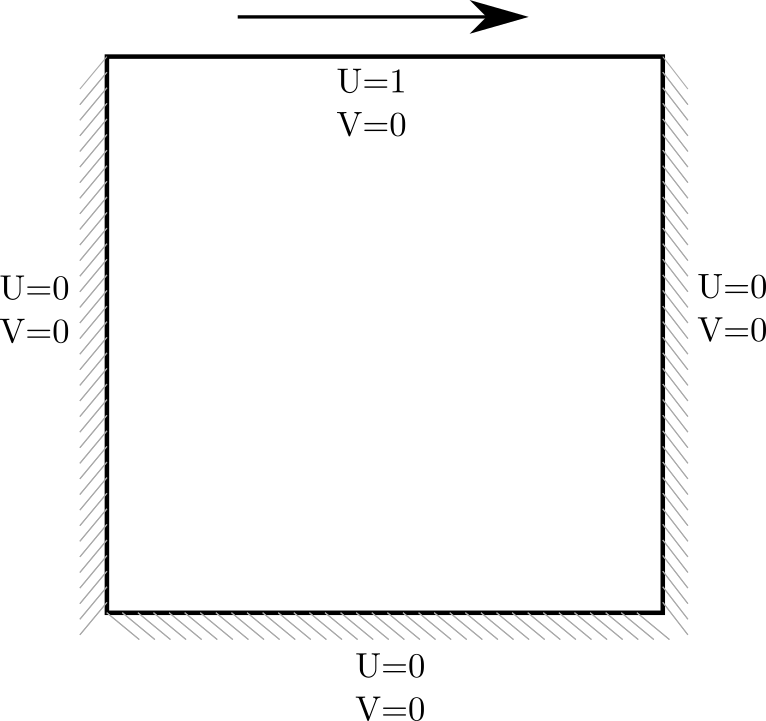
\includegraphics[width=0.4\linewidth]{cavity2d.png}
\caption{Область расчёта задачи о каверне}
\label{fig:cavity}
\end{figure}

Задача реализована в тесте \ename{[cavity2-simple]} в файле \ename{cavity_simple_test.cpp}.

Программа проводит итерации стартуя от начального нулевого состояния
$u=v=p=0$ до тех пор, пока невязка не достигнет заданного порога.
На каждой итерации поле давления и векторное поле скорости сохраняются
на основной сетке в файл \ename{cavity2.vtk.series}.

Итоговый результат (для $\eps=10^{-2}$) представлен на \figref{fig:cavity-result}.

\begin{figure}[h]
\centering
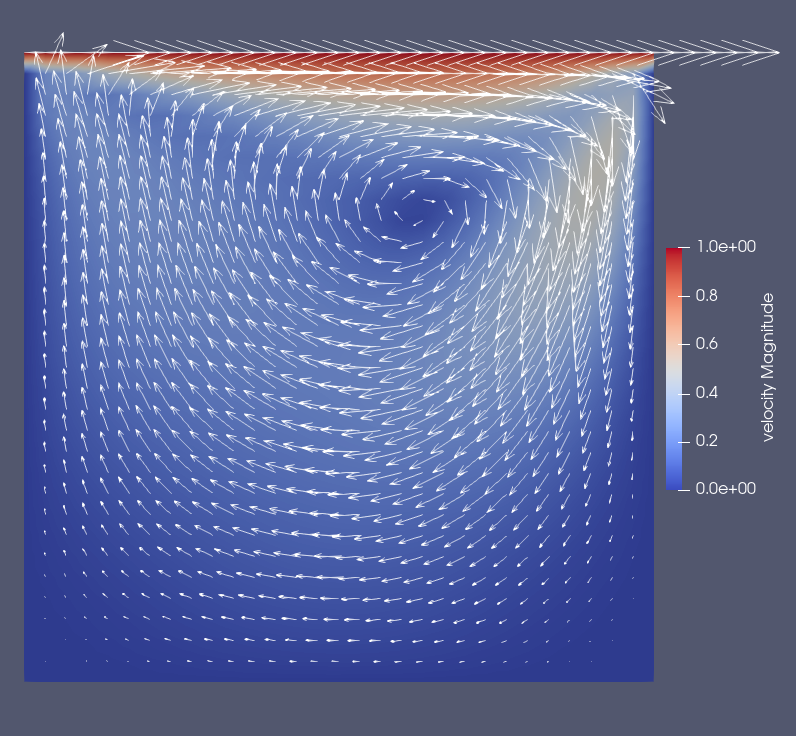
\includegraphics[width=0.7\linewidth]{cavity2d-result.png}
\caption{Область расчёта задачи о каверне}
\label{fig:cavity-result}
\end{figure}

Для отображения вектора поля скорости в Paraview см. справку в \ref{sec:paraview-glyph}.

Для работы с разнесённой сеткой в классе \cvar{cfd::RegularGrid2D}
представлены функции
\begin{itemize}
\item \cvar{cfd::RegularGrid2D::cell_centered_grid()}  -- построить сетку по центрам ячеек (``чёрную'' сетку для $p$),
\item \cvar{cfd::RegularGrid2D::xface_centered_grid()} -- построить сетку по центрам $x$-граней (``синюю'' сетку для $v$),
\item \cvar{cfd::RegularGrid2D::yface_centered_grid()} -- построить сетку по центрам $y$-граней (``красную'' сетку для $u$),
\end{itemize}

и функции перевода индексов
\begin{itemize}
\item \cvar{cfd::RegularGrid2D::cell_centered_grid_index_ip_jp} -- посчитать линейный индекс ``чёрной'' сетки \eqref{eq:ns2d_kipjp},
\item \cvar{cfd::RegularGrid2D::xface_grid_index_ip_j} -- посчитать линейный индекс ``синей'' сетки \eqref{eq:ns2d_kipj},
\item \cvar{cfd::RegularGrid2D::yface_grid_index_i_jp} -- посчитать линейный индекс ``красной'' сетки \eqref{eq:ns2d_kijp}.
\end{itemize}

\subsubsection{Функция верхнего уровня}
\clisting{open}{"test/cavity_simple_test.cpp"}
\clisting{line}{"[cavity2-simple]"}

Сначала устанавливаются параметры задачи:
число Рейнолдса,
\clisting{line}{"Re"}
параметры алгоритма SIMPLE,
\clisting{lines-range}{"tau", "alpha"}
разбиение сетки, 
\clisting{line}{"n_cells"}
максимальное количество итераций 
\clisting{line}{"max_it"}
и значение невязки, при котором итерации прекращаются
\clisting{line}{"double eps"}

Затем происходит инициализация решателя, который
определён в классе \cvar{Cavity2DSimpleWorker}
\clisting{line}{"Cavity2DSimpleWorker"}
и параметров сохранения. Здесь
первым параметром является флаг сохранения
точных сеточных значений, который установлен в \cvar{false},
а также имя файла с итоговым результатом.
Таким образом сохраняться будет только решение,
интерполированное на основную сетку.
Для целей отладки программы (для просмотра действительных, не интерполированных полей решения)
следует первый флаг установить в \cvar{true}. Тогда помимо \ename{cavity2.vtk.series}, будут
создаваться также файлы \ename{cavity2-u}, \ename{cavity2-v}, \ename{cavity2-p}.
\clisting{until}{"_saver"}

Потом происходит установка начальных значений искомых сеточных векторов: $u=v=p=0$
\clisting{lines-range}{"u_init", "set_uvp"}

и начинается итерационный процесс.
\clisting{line}{"for"}

Внутри цикла
выполняется шаг итерационного процесса, который
возвращает значение итоговой невязки в переменную \cvar{nrm}.
\clisting{line}{"step"}

На печать выводится индекс итерации, значение невязки и значение давления в правом верхнем узле (для контроля сходимости)
\clisting{line}{"cout"}

Сохраняется состояние решателся на пройденную итерацию
\clisting{line}{"save_current"}

и производится проверка на сходимость
\clisting{block}{"if (nrm < eps)"}

В конце производится проверка: при установленных параметрых решение
должно сойтись за 9 итераций:
\clisting{line}{"CHECK"}

\subsubsection{Поля класса решателя}
\clisting{to-start}{}
Класс \cvar{Cavity2DSimpleWorker} хранит в себе набор полей,
характеризующих состояние итерационного процесса.
Некоторые из этих полей (параметры решателя) постоянны (\cvar{const}) и
определяются непосредственно перед вызовом конструктора в инициализаторе. Другие
меняются с продвижением по итерациям.

Среди постоянных полей заданы 4 сетки: основная \cvar{_grid},
``чёрная'' сетка \cvar{_cc_grid} (cell-centered) для давления,
``красная'' сетка \cvar{_yf_grid} (y-face) для $u$,
``синяя'' сетка \cvar{_xf_grid} (x-face) для $v$ (\figref{fig:staggered_grid}).
\clisting{pass}{"private"}
\clisting{until}{"_yf_grid"}
Далее заданы скалярные параметры: число Рейнольдса, шаги сетки и параметры алгоритма SIMPLE
\clisting{until}{"_alpha_p"}

Далее следуют сеточные вектора, характеризующие текущее состояние решателя:
найденные на последней итерации давление и скорости.
\clisting{until}{"_v;"}

Также определяется данные для решения системы уравнений для нахождения $p'$ \eqref{eq:ns2d_pprime_slae}:
значения $d^u, d^u$, а так же инициализированный решатель системы уравнений.
Поскольку используется постоянные шаги по времени, $d^u, d^v$ являются скалярами.
\clisting{until}{"_p_prime_solver"}

Хранятся левая и правая части систем уравнений \eqref{eq:ns2d_ustar_slae}, \eqref{eq:ns2d_vstar_slae}
для определения пробных значений скорости и расчета невязки.
\clisting{until}{"_rhs_v;"}

Указатели на классы, помогающие сохранять найденные вектора в vtk - формат.
Эти классы инициализируются только в случае, если пользователь указал на 
необходимость сохранения.
\clisting{until}{"_writer_all;"}

\subsubsection{Инициализация решателя}
\clisting{to-start}{}

В секции инициализации конструктора
созаются сетки в единичном квадрате и переписываются параметры решения.
Далее в теле конструктора вычисляются значения
$d^u, d^v$ по формулам \eqref{eq:ns2d_du}, \eqref{eq:ns2d_dv}
и собирается решатель для $p'$. Как было указано ранее,
матрица системы $A^p$ не меняется
с продвижением по итерациям, поэтому этот решатель можно собрать один раз
до начала счёта.

\clisting{block}{"Cavity2DSimpleWorker::Cavity2DSimpleWorker"}

Начальные значения устанавливаются через вызов функции \cvar{set_uvp}.
Эти начальные значения будут использоваться в качестве значений
с предыдущего итерационного слоя на первой итерации.

В функции происходит переписывание переданных векторов
в приватные поля класса.
\clisting{lines-range}{"set_uvp", "_p"}

После этого данных в классе-решателе достаточно,
для сборки матриц $A^u, A^v$ и правых частей
$b^u, b^v$ для системы уравнений \eqref{eq:ns2d_ustar_slae}, \eqref{eq:ns2d_vstar_slae}.
\clisting{until}{"v_slae()"}

Если посмотреть на выражение для невязки \eqref{eq:ns2d_residual} убрав в нём крышки над переменными, то можно
убедится, что оно аппроксимируется в виде
\begin{equation*}
    r_u = \frac{1}{\tau}\left(A^u u - b^u\right).
\end{equation*}
Поэтому после сборки систем уравнений движения, можно вычислить невязку, характеризующую
отклонение установленного в этой процедуре решения от желаемого:
\clisting{until-close}{}

\subsubsection{Шаг итерации SIMPLE}
\clisting{to-start}{}
Осуществляется в процедуре
\clisting{block}{"double Cavity2DSimpleWorker::step()"}
и представляет собой буквальное пошаговое следование алгоритму SIMPLE (\ref{sec:simple-algo}).
В конце опять вызывается функция \cvar{set_uvp} для сборки матриц для следующей итерации
и подсчёта невязки на текущей итерации.

\subsubsection{Сборка системы уравнений для поправки давления}
\clisting{to-start}{}

Сборка системы уравнений \eqref{eq:ns2d_pprime_slae}
осуществляется в процедуре
\clisting{line}{"void Cavity2DSimpleWorker::assemble_p_prime_solver()"}
Сборка происходит с использованием матрицы формата \cvar{cfd::LodMatrix},
удобного для непоследовательной записи.
\clisting{until}{"LodMatrix"}
Заполнение происходит в цикле по раздвоенным индексам $ij$
``чёрной'' сетки для давления:
\clisting{until}{"size_t i"}
Внутри цикла устанавливаются флаги, характеризующие граничный статус текущего узла
\clisting{until}{"is_top"}
Вычисляется значение сквозного индекса по формуле \eqref{eq:ns2d_kipjp}
\clisting{until}{"ind0"}
и значения коэффициентов в формулах \eqref{eq:ns2d_ap}. Поскольку
сетка равномерная, эти значения не меняются для разных узлов
\clisting{until}{"coef_y"}
Далее формулы \eqref{eq:ns2d_ap}
применяются для заполнения матриц
с учётом аппроксимированного граничного условия \eqref{eq:ns2d_bc3}.
Так, запись
\clisting{until-close}{}
для всех неправых узлов с линейным индексом \cvar{ind0} вычисляет индекс 
узла, расположенного правее него с линейным индексом \cvar{ind1},
добавляет слагаемое в диагональный (первое из уравнений \eqref{eq:ns2d_ap}) и
вычитает из недиагонального (четвёртое из уравнений \eqref{eq:ns2d_ap}) элемента
строки \cvar{ind0}.
Для правых узлов работает граничное условие \eqref{eq:ns2d_ap} и выполнять эту процедуру
не нужно.

После заполнения в матрицу вводится граничное условие \eqref{eq:ns2d_bc4}
\clisting{line}{"set_unit_row"}

И матрица передаётся в решатель СЛАУ предварительно сконверованная в формат \cvar{cfd::CsrMatrix}
\clisting{until}{"set_matrix"}

Правая часть собирается заново на каждой итерации по формуле \eqref{eq:ns2d_bp}.
Её реализация представлена в функции
\clisting{line}{"Cavity2DSimpleWorker::compute_p_prime"}
Сначала собирается правая часть системы \eqref{eq:ns2d_pprime_slae} по формуле \eqref{eq:ns2d_bp}:
\clisting{block}{"for (size_t i"}
потом осуществляется установка граничного условия \eqref{eq:ns2d_bc4}
\clisting{line}{"rhs[0]"}
и вызывается решатель СЛАУ
\clisting{until-close}{}

\subsubsection{Сборка системы уравнений для пробной скорости}
\clisting{to-start}{}

Сборка системы \eqref{eq:ns2d_ustar_slae} (как правой, так и левой частей) реализована
в функции
\clisting{line}{"Cavity2DSimpleWorker::assemble_u_slae"}

Основной цикл идёт по негрничным узлам ``красной'' сетки,
в котором реализуются формулы \eqref{eq:ns2d_au}
\clisting{pass}{"internal"}
\clisting{block}{"for (size_t", "rhs"}

Как было отмечено в пункте \ref{sec:simple-bc},
граничные условия первого рода в этом уравнении
учитываются двумя разными способами:
узлы расположенные непосредственно на границе (нижней и верхней)
учитываются по схеме \eqref{eq:ns2d_bc1}, которая реализована в цикле
\clisting{to-start}{}
\clisting{block}{"for (size_t j=0; j< _grid.ny(); ++j)"}

А фиктивные узлы, возникающие при обработке
узлов расположенных в полушаге от границ (левой и правой),
обрабатываются по схеме \eqref{eq:ns2d_bc2}.
Эта схема реализована в виде
препроцессинга алгоритма добавления элемента в матрицу в лямбда-функции
\clisting{to-start}{}
\clisting{pass}{"assemble_u_slae"}
\clisting{block}{"add_to_mat"}

Эта лямбда вызывается везде, где нужно добавить в строку \cvar{row_index}
и колонку, соответствующую узлу \cvar{ij_col}, значение \cvar{value}.
Она перехватывает ситуации с ``фиктивным'' узлом ($j=-1, j=n_y$)
и применяет алгоритм \eqref{eq:ns2d_bc2}.


\subsection{Задание для самостоятельной работы}

\begin{enumerate}

\item 
Подобрать оптимальные параметры алгоритма SIMPLE $\tau, \alpha_p$ для задачи в каверне,
при которых сходимость происходит за наименьшее число итераций.
Для этого лучше понизить пороговый $\eps=0.01$.
Сравнить полученные вами эмпирически значения с рекомендованными.
Увеличить разбиение и отметить, как величина шага по простравнству влияет на количество
требуемых итераций.
Для ускорения параметрических расчётов лучше собирать программу в ``релизной'' (\ref{sec:release-build}) 
версии и убрать сохранение в vtk внутри каждой итерации.

\item
Нарисовать поле невязок $r_u, r_v$ в динамике по каждой итерации. Отметить в каком из уравнений и в каких местах области расчёта
наблюдаются наибольшие проблемы со сходимостью.
Обратить внимание, что невязка $r_u$ задана на ``красной'' сетке. При этом сохранение на этой сетке делается
через объект \cvar{_writer_u}. Невязка $r_v$ задается на ``синей'' сетке с объектом сохранения \cvar{_writer_v}.

\item
Решить аналогичную задачу, в которой скорость не только на верхней, но и на
нижней стенке равна $U=1$. Для этого завести новый тест \ename{[cavity2-simple-sym]}.

\end{enumerate}

\section{Лекция 18 (30.11)}

\subsection{Нестационарное уравнение Навье-Стокса}
\label{sec:ns2d-nonstat}

Запишем безразмерную систему \eqref{eq:ns2d_u} -- \eqref{eq:ns2d_div} в нестационарной постановке
\begin{equation}
\label{eq:ns2d_nonstat}
\begin{array}{l}
    \ddfr{u}{t} + \ddfr{u^2}{x} + \ddfr{uv}{y} =
        -\ddfr{p}{x}
        + \dfrac{1}{\Ren}\left(\ddfrq{u}{x} + \ddfrq{u}{y}\right),\\[10pt]
    \ddfr{v}{t} + \ddfr{uv}{x} + \ddfr{v^2}{y} =
        -\ddfr{p}{y}
        + \dfrac{1}{\Ren}\left(\ddfrq{v}{x} + \ddfrq{v}{y}\right), \\[10pt]
    \ddfr{u}{x} + \ddfr{v}{y} = 0.
\end{array}
\end{equation}
Характерное время, на которое было произведено обезразмериваение,
равно $t^0 = L/U$.

\subsubsection{Cхема расчёта по алгоритму SIMPLE}
\label{sec:simple-nonstat-algo}

Производную по времени будет аппроксимировать по двухслойной неявной схеме.
\begin{equation*}
\dfr{u}{t} = \frac{\hat u - \check u}{\dt} + o(\dt),
\end{equation*}
где символом $\check\cdot$ обозначены значения с предыдущего временн\'{о}го слоя.

Внутри каждого временн\'{о}го слоя будем исполнять
итерационный процесс по типу \eqref{eq:ns2d_semi_u} -- \eqref{eq:ns2d_semi_div}
с добавлением дискретизованной производной по времени:

\begin{equation}
    \label{eq:ns2d_nonstat_semi}
    \begin{array}{l}
    \displaystyle
    \frac{\hat u - \check u}{\dt} + \frac{\hat u - u}{\tau} + \dfr{u \hat u}{x} + \dfr{v \hat u}{y} =
        -\dfr{\hat p}{x}
        + \frac{1}{\Ren}\left(\dfrq{\hat u}{x} + \dfrq{\hat u}{y}\right), \\[10pt]
    \displaystyle
    \frac{\hat v - \check v}{\dt} + \frac{\hat v - v}{\tau} + \dfr{u\hat v}{x} + \dfr{v \hat v}{y} =
        -\dfr{\hat p}{y}
        + \frac{1}{\Ren}\left(\dfrq{\hat v}{x} + \dfrq{\hat v}{y}\right),  \\[10pt]
    \displaystyle
    \dfr{\hat u}{x} + \dfr{\hat v}{y} = 0.
    \end{array}
\end{equation}

Далее на основе этих уравнений проведём рассуждения, аналогичные приведённым в п. \ref{sec:simple-algo}.
Уравнения для пробной скорости типа \eqref{eq:ns2d_ustar}, \eqref{eq:ns2d_vstar}
примут вид
\begin{equation}
    \label{eq:ns2d_nonstat_uvstar}
    \begin{array}{l}
    \displaystyle
    \left(1 + \frac{\tau}{\dt}\right)u^* + \tau\dfr{u u^*}{x} + \tau\dfr{v u^*}{y}
       - \frac{\tau}{\Ren}\left(\dfrq{u^*}{x} + \dfrq{u^*}{y}\right)
       = -\tau\dfr{p}{x} + u + \frac\tau\dt \check u, \\[10pt]
    \displaystyle
    \left(1 + \frac{\tau}{\dt}\right)v^* + \tau\dfr{u v^*}{x} + \tau\dfr{v v^*}{y}
       - \frac{\tau}{\Ren}\left(\dfrq{v^*}{x} + \dfrq{v^*}{y}\right)
       = -\tau\dfr{p}{y} + v + \frac\tau\dt \check v.
   \end{array}
\end{equation}

Уравнения для поправок скорости \eqref{eq:ns2d_uprime_approx}, \eqref{eq:ns2d_vprime_approx}
и давления \eqref{eq:ns2d_pprime_diff}
можно оставить в неизменном виде если модифицировать входящие в них множители $d^u, d^v$.
По аналогии с \eqref{eq:ns2d_du}, \eqref{eq:ns2d_dv} запишем
\begin{equation}
    \label{eq:ns2d_nonstat_duv}
    \begin{array}{l}
    \displaystyle
    d^u = \left({\rm diag}\left(S^u\right)\right)^{-1} = 
        \left(1 + \frac\tau\dt + \frac{2\tau}{\Ren}\left(\frac{1}{h_x^2} + \frac{1}{h_y^2}\right)\right)^{-1} \\[10pt]
    \displaystyle
    d^v = \left({\rm diag}\left(S^v\right) \right)^{-1}= 
        \left(1 + \frac\tau\dt + \frac{2\tau}{\Ren}\left(\frac{1}{h_x^2} + \frac{1}{h_y^2}\right)\right)^{-1}.
    \end{array}
\end{equation}
Здесь $S^u$, $S^v$ -- матрицы левых частей выражений \eqref{eq:ns2d_nonstat_uvstar}.

Схема расчёта на временн\'{о}м слое остаётся аналогичной стационарному случаю,
с той разницей, что первая итерация использует значение расчётных полей
с предыдущего шага по времени.
Порядок действий на временном слое:

\begin{enumerate}
\item Присвоить $u=\check u$, $v=\check v$, $p=\check p$;
\item Из уравнений \eqref{eq:ns2d_nonstat_uvstar}
      вычислить значения $u^*, v^*$;
\item Определить поправку давления $p'$ из уравнения \eqref{eq:ns2d_pprime_diff} с использованием \eqref{eq:ns2d_nonstat_duv};
\item Найти поправки скорости $u', v'$ из выражений \eqref{eq:ns2d_uprime_approx}, \eqref{eq:ns2d_vprime_approx} с использованием \eqref{eq:ns2d_nonstat_duv};
\item Выразить значения переменных для текущего слоя из \eqref{eq:ns2d_decomp};
      Для определения давления использовать сглаживание с коэффициентом $\alpha_p$;
\item Найти невязку с ипользованием найденных значений $\hat u, \hat v, \hat p$
      из выражения \eqref{eq:ns2d_residual}.
      Если она недостаточно мала, то выполняется присваивание
      $u = \hat u, \; v=\hat v, \; p = \hat p$ 
      и возвращение на шаг 2.
      Если сходимость достигнута, то перейти на следующий шаг по времени.
      Для этого выполнить
      $\check u = \hat u, \; \check v= \hat v, \; \check p = \hat p$ 
      и перейти на шаг 1.
\end{enumerate}

\subsection{Задача об обтекании препятствия}
\label{sec:problem-obstacle}

\subsubsection{Расчётная сетка}
Рассмотрим постановку граничных условий и особенности пространственной аппроксимации для задачи
о внешнем обтекании. Поскольку рассматриваемые нами методы
пока ограничены аппроксимациями на структурированной прямоугольной
сетке, то будем рассматривать такую область расчёта,
которую легко можно отобразить на такой сетке. Пусть внешняя
область расчёта и обтекаемое препятствие представляет из себя прямоугольники.

\begin{figure}[h!]
\centering
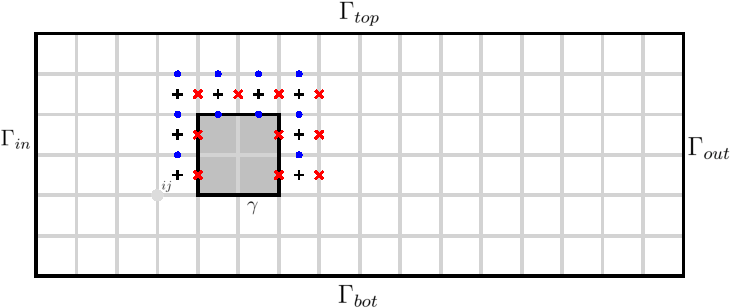
\includegraphics[width=0.8\linewidth]{obstacle_staggered.pdf}
\caption{Область расчёта и разнесённая сетка для задачи обтекания}
\label{fig:obstacle_staggered}
\end{figure}

По аналогии с \figref{fig:staggered_grid} введём в этой области
прямоугольную сетку (\figref{fig:obstacle_staggered}).

В случае сохранения естестественной нумерации узлов и ячеек сетки
часть их этих пронумерованных ячеек выпадает из области расчёта (попадает внутрь препятствия).
Для таких случаев существует два способа работы с нумерацией:
\begin{itemize}
\item
Можно сохранить естественную нумерацию, при этом часть ячеек пометить
как неактивные (например, введя специальный массив признаков \ename{actnum},
$i$-ый элемент которого равен единице для активной ячейки и нулю для неактивной).
Количество элементов в сеточных векторах тогда будет равно общему количеству
всех ячеек (и активных и неактивных). Но значения этих векторов в неактивных ячейках будут фиктивными (нулями).
\item
Можно нумеровать лишь активные ячейки (и узлы), тем самым
нарушив естественную нумерацию. 
\end{itemize}

Оба этих подхода имеют свои очевидные плюсы и минусы.
Первый подход сохраняет простые зависимости для перевода двумерного индекса в сквозной и
диагональную структуру сеточных матриц. Второй подход более экономичен в хранении данных. 

\subsubsection{Граничные условия}
Рассмотрим постановку со следующими граничными условиями:
\begin{itemize}
\item
во входном сечении зададим равномерный профиль скорости
\begin{equation}
\label{eq:ns2d_obstable_bc_in}
(x, y) \in \Gamma_{in}: u=1, \; v=0;
\end{equation}
\item
на нижней и верхней границах -- условие симметрии (идеального скольжения). Это условие моделирует
зеркальное отражение расчётной области относительно соответствующих границ $\Gamma_{top}, \Gamma_{bot}$.
\begin{equation}
\label{eq:ns2d_obstable_bc_topbot}
(x, y) \in \Gamma_{top}, \Gamma_{bot}: \dfr{u}{n}=0, \; v = 0;
\end{equation}
\item
на самом обтекаемом деле -- условия прилипания
\begin{equation}
\label{eq:ns2d_obstable_bc_wall}
(x,y) \in \gamma: u=0, \; v=0;
\end{equation}
\item
в выходном сечении -- условия выхода потока. Их точную формулировку определим позднее.
\end{itemize}

На каждом шаге алогоритма SIMPLE требуется
решить три дифференциальных уравнения \cref{eq:ns2d_ustar,eq:ns2d_vstar,eq:ns2d_pprime_diff}.
относительно неизвестных $u^*, v^*, p'$.
Значит из представленных выше граничных условий требуется
выразить граничные значения для этих трёх неизвестных сеточных векторов
и расписать способ их учёта при сборке соответствующих систем линейных уравнений.

\subsubsubsection{Входное сечение}
\label{sec:obstacle_bc_input}
При разложении скорости на пробное значение и поправку \cref{eq:ns2d_decomp}
условия для скорости \cref{eq:ns2d_obstable_bc_in} раскладываются следующим образом:
\begin{equation}
\label{eq:ns2d_decomp_input}
(x,y) \in \Gamma_{in}: u^* = 1, \; v^* = 0, \; u' = v' = 0
\end{equation}
Условия первого рода для пробной скорости учитываются при решении уравнений
\cref{eq:ns2d_ustar,eq:ns2d_vstar}.
Для сеточного вектора $u^*$, узлы которого лежат непосредственно на границе,
учёт этого условия сводится к модификации соответствующей строки матрицы $A^u$ и правой части $b^u$.
В строке $k=k\left[0, j+\tfrac12\right]$:
\begin{equation}
\label{eq:ns2d_au_bc_left}
A^u_{km} = \delta_{km}, \quad b^u_k = 1.
\end{equation}

Для сеточного вектора $v^*$ учёт производится с помощью выражения для значения в фиктивном узле $k_1 = k\left[-\tfrac12, j\right]$
через значение в настоящем узле $k_0 = k\left[\tfrac12, j\right]$:
$$
\frac{v^*_{k_0} + v^*_{k_1}}{2} = 0 \hence v^*_{k_1} = -v^*_{k_0}.
$$
Поэтому при сборке матрицы $A^v$ по формулам \cref{eq:ns2d_av} при необходимости добавить
значение $a$ в колонку, соответствующую фиктивному узлу, требуется добавить это значение
в диагональ с обратным знаком:
\begin{equation}
\label{eq:ns2d_av_bc_left}
A^v_{k_0, k_1} {{+}{=}} a \hence A^v_{k_0, k_0} \minuseq a
\end{equation}

Из условий на поправку скорости $u'=v'=0$ и уравнений \cref{eq:ns2d_uprime_approx,eq:ns2d_vprime_approx}
следует граничное условие для поправки давления
\begin{equation}
\label{eq:ns2d_obstacle_bc_pres}
x,y\in\Gamma_{in}: \dfr{p'}{x}=0
\end{equation}
Из этого условия получаем соотношение для давления в фиктивном узле $k_1 = k\left[-\tfrac12, j+\tfrac12\right]$
через значение  в реальном узле $k_0 = k\left[\tfrac12, j+\tfrac12\right]$:
$$
p'_{k_1} = p'_{k_0}
$$
Тогда добавление значения $a$ в фиктивную колонку $k_1$ эквивалентно
\begin{equation}
\label{eq:ns2d_ap_bc}
A^p_{k_0, k_1} {{+}{=}} a \hence A^p_{k_0, k_0} \pluseq a
\end{equation}

Следует понимать, что выражение \cref{eq:ns2d_uprime_approx}
является приближением, используемым в расчётной схеме SIMPLE.
В действительности, использование условия \cref{eq:ns2d_obstacle_bc_pres} (в случае нулевого начального приближения давления)
приводит к нулевой производной для всего давления (а не только поправки)
$$
x,y\in\Gamma_{in}: \dfr{p}{x}=0.
$$
Это выражение никак не следует из постановки задачи.
Действительно, если расписать уравнение \cref{eq:ns2d_u} с учётом условий \cref{eq:ns2d_obstable_bc_in}
и уравнения неразрывности \cref{eq:ns2d_div}, то получим соотношение
\begin{equation}
\label{eq:ns2d_obstacle_true_bc_p}
x,y\in\Gamma_{in}: \dfr{p}{x} = \frac{1}{\Ren}\dfrq{u}{x} = -\frac1\Ren\dfr{}{x}\left(\dfr{v}{y}\right).
\end{equation}
(при выводы учтено, что $\dsfr{v}{y} = -\dsfr{u}{x} = 0$).
Однако, практика показывает, что в большинстве случаев, условий типа \cref{eq:ns2d_obstacle_bc_pres}
оказывается достаточно. Выражение \cref{eq:ns2d_obstacle_true_bc_p} равно нулю,
если поперечная компонента скорости не появляется сразу за входным сечением. То есть
течение остается прямолинейным на начальном участке расчётной области.
Чтобы это исполнялось, входное сечение необходимо размещать
на таком растоянии от препятствия, на котором поток еще не чувствует его присутствия (не начинает разворачиваться).

\subsubsubsection{Условия симметрии}
Однородные условие для скорости \cref{eq:ns2d_obstable_bc_topbot} расписываются
как
$$
(x,y) \in \Gamma_{in}: \dfr{u^*}{y} = \dfr{u'}{y} = 0, \; v^* = v' = 0.
$$
Из условия на $u^*$ запишем соотношение для фиктивного узла около нижней границы, которое будем использовать
при сборке матрицы $A^u$:
\begin{align*}
&k_0 = k\left[i+\tfrac12, \tfrac12\right], \quad k_1 = k\left[i+\tfrac12, -\tfrac12\right], \\
&u^*_{k_1} = u^*_{k_0}, \\
&A^u_{k_0, k_1} {{+}{=}} a \hence A^u_{k_0, k_0} \pluseq a.
\end{align*}
Условие на $v^*$ можно использовать явно:
\begin{align*}
&k = k\left[i+\tfrac12, \tfrac12\right], \\
&A^u_{k,s} = \delta_{ks}, \quad b^u_k = 0.
\end{align*}

Граничное условие для поправки давления
можно получить из уравнения движения \cref{eq:ns2d_v} (в неконсервативном виде) с учётом уравнения неразрывности.
Используя
\begin{align*}
&(x,y) \in \Gamma_{top,bot}:
	v = 0 \hence \dfr{v}{x} = 0 \hence \dfrq{v}{x} = 0,\\
&\phantom{(x,y) \in \Gamma_{top,bot}}:
	\dfr{u}{y} = 0 \hence \dfr{}{x}\dfr{u}{y} = 0 \hence \dfrq{v}{y} = 0,\\
\end{align*}
получим
$$
(x,y) \in \Gamma_{top,bot}: \dfr{p}{y} = 0.
$$
При использовании нулевого начального приближения давления, для поправки давления так же справедливо
$$
(x,y) \in \Gamma_{top,bot}: \dfr{p'}{y} = 0.
$$
Учёт этого условия на матричном уровне аналогичен процедуре \cref{eq:ns2d_ap_bc}.

\subsubsubsection{Условия прилипания}
\label{sec:obstacle-noslip}
Учёт условий прилипания на границе обтекаемого тела \cref{eq:ns2d_obstable_bc_wall}
в целом аналогичен алгоритму учёта входной границы.
Для компонент скорости, узлы которых лежат на границе работает процедура \cref{eq:ns2d_au_bc_left} (с нулём в правой части).
В случае если узлы не лежат на границе, то используется процедура \cref{eq:ns2d_av_bc_left}.

Для поправки давления так же используется однородное условие второго рода \cref{eq:ns2d_obstacle_bc_pres}
И все комментарии к этому условию, указанные в пункте \ref{sec:obstacle_bc_input}, остаются справедливыми.

\subsubsubsection{Выходные граничные условия}
На выходной границе отсутствует возможность указать какие-либо физичные условия для искомых переменных.
При этом, как правило, поведение течения в этой области большого интереса не представляет.
Поэтому здесь требуется написать такие выражения, учёт которых
не оказывал бы влияния на течение в основной области расчёта.
Отсюда возникает проблема формулировки неотражающих граничных условий.
Цель состоит в том, чтобы жидкость выходила из области расчёта естественным для себя образом, не подстраиваясь под выходную границу.

Простейшим решением этой проблемы является использование уравнения переноса на выходной границе:
\begin{equation}
\label{eq:ns2d_outflow_common}
\begin{aligned}
(x,y)\in\Gamma_{out}:\; &\dfr{u}{t} + u\dfr{u}{x} = 0,\\[10pt]
                        &\dfr{v}{t} + u\dfr{v}{x} = 0.
\end{aligned}
\end{equation}
В стационарном случае ($\dsfr{u,v}{t} = 0$) из этих условий следует, что поперечная скорость равна нулю:
\begin{equation*}
\dfr{u}{x} = 0 \hence \dfr{v}{y} = 0 \hence v = v|_{\Gamma_{bot}} = 0.
\end{equation*}

По аналогии с уравнениями движения \cref{eq:ns2d_semi_u}
в уравнение на выходной границе так же добавим фиктивную производную по времени.
Тогда условия для компонент скорости на итерации SIMPLE примут вид (для стационарного случая)

\begin{equation}
\label{eq:ns2d_outflow_common_semi}
\begin{aligned}
(x,y)\in\Gamma_{out}:\; &\frac{\hat u - u}{\tau} + u\dfr{\hat u}{x} = 0,\\[10pt]
                        &\hat v = 0.
\end{aligned}
\end{equation}

Подставим разложение \cref{eq:ns2d_decomp} и запишем условия для уравнений пробной скорости

\begin{align}
\label{eq:ns2d_outflow_ustar}
(x,y)\in\Gamma_{out}:\; &u^* + \tau u\dfr{u^*}{x} = u,\\[10pt]
\label{eq:ns2d_outflow_vstar}
                        &v^* = 0.
\end{align}

Пробная скорость в алгоритме SIMPLE не удовлетворяет уравнению неразрывности.
Поэтому нет гарантий, что найденная $u^*$ сохраняет баланс масса в расчётной области.
На практике это означает, что количество жидкости, которое втекает через $\Gamma_{in}$ не равно
количеству жидкости, которое вытекает через $\Gamma_{out}$.

Но финальная по итогам SIMPLE итерации скорость должна сохранять баланс массы.
То есть
$$
\triangle Q = \int_{\Gamma_{in}} \hat u \, ds - \int_{\Gamma_{out}} \hat u \, ds = 0.
$$
Раскладывая это выражение через пробную скорость и поправку с учётом нулевого значения $u'$ на входной границе \cref{eq:ns2d_decomp_input},
получим
$$
\int_{\Gamma_{out}} u' \, ds = \int_{\Gamma_{in}} u^* \, ds - \int_{\Gamma_{out}} u^* \, ds
$$
Положим, что $u'$ на выходной границе постоянна.
Это предположение не влияет на итоговый результат SIMPLE итераций, так как
при его сходимости поправки скорости обнуляются. Тогда запишем значение поправки скорости
на выходной границе
\begin{equation}
\label{eq:ns2d_uprime_from_balance}
(x,y)\in\Gamma_{out}:\; u' = \left(\int_{\Gamma_{in}} u^* \, ds - \int_{\Gamma_{out}} u^* \, ds \right) / \left|\Gamma_{out}\right|
\end{equation}
Подставляя это выражение в \cref{eq:ns2d_uprime_approx}, получим граничные условия на поправку давления
\begin{equation}
\label{eq:ns2d_outflow_pprime}
(x,y)\in\Gamma_{out}:\;  d^u\dfr{p'}{x} = -\frac{u'}{\tau}
\end{equation}

Таким образом, мы вывели граничные условия для всех трёх дифференциальных уравнений:
\cref{eq:ns2d_outflow_ustar,eq:ns2d_outflow_vstar,eq:ns2d_outflow_pprime}.

Отметим, что если выходных границ несколько, то выражение \cref{eq:ns2d_uprime_from_balance}
следует записывать для каждой из границ. При этом следует дополнительно задавать
долю расхода $C_i$, вытекающую через каждую из границ. Пусть $\Gamma_{out} = \Gamma_{o1} \cap \Gamma_{o2}$.
Тогда
\begin{align*}
&(x,y)\in\Gamma_{o1}:\; u' = \left(C_1 \int_{\Gamma_{in}} u^* \, ds - \int_{\Gamma_{o2}} u^* \, ds \right) / \left|\Gamma_{o1}\right|\\
&(x,y)\in\Gamma_{o2}:\; u' = \left(C_2 \int_{\Gamma_{in}} u^* \, ds - \int_{\Gamma_{o1}} u^* \, ds \right) / \left|\Gamma_{o2}\right|\\
&C_1 + C_2 = 1.
\end{align*}

\paragraph{Учёт условия для $u^*$ \cref{eq:ns2d_outflow_ustar}}
Просто перепишем уравнение в строках СЛАУ, соответствующих выходным узлам $k_0 = k\left[n_x, j+\tfrac12\right]$.
Для этого аппроксимируем конвективную производную по схеме против потока (с противопоточным узлом
$k_1 = k\left[n_x-1, j+\tfrac12\right]$).
$$
u^*_{k_0} + \tau U_{k_0} \frac{u^*_{k_0} - u^*_{k_1}}{h_x} = u_{k_0},
$$
где $U$ - скорость переноса в $k_0$-ом узле. Она должна быть всегда больше нуля (иначе схема
перестаёт быть противопотоковой). Можно просто положить её равной среднерасходной (единице в нашем случае).
А можно взять из предыдущей итерации с проверкой на положительность:
$$
U_{k_0} = \max\left(0, u_{k_0}\right).
$$
На матричном уровне получим:
\begin{equation}
\label{eq:ns2d_outflow_ustar_mat}
\begin{aligned}
&A^u_{k0, s} = \begin{cases}
	1 + \dfrac{\tau U_{k_0}}{h_x}, \quad s = k_0\\[10pt]
	-\dfrac{\tau U_{k_0}}{h_x}, \quad s = k_1\\[10pt]
	0, \quad \text{иначе},
\end{cases}, \\
&b^u_{k_0} = u_{k_0}
\end{aligned}
\end{equation}

\paragraph{Учёт условия для $v^*$ \cref{eq:ns2d_outflow_vstar}}
будем осуществлять за счёт введения фиктивного узла:
\begin{align*}
&k_0 = k\left[n_x - \tfrac12, j\right], \; k_1 = k\left[n_x + \tfrac12, j\right], \\
&\frac{v^*_{k_0} + v^*_{k_1}}{2} = v^*_{\Gamma_{out}} = 0 \hence v^*_{k_1} = -v^*_{k_0}.
\end{align*}
Отсюда добавление элемента $a$ в фиктивную колонку будет осуществляться в виде
$$
A^v_{k_0, k_1} \pluseq a \hence A^v_{k_0, k_0} \minuseq a.
$$


\paragraph{Учёт условия для $p'$ \cref{eq:ns2d_outflow_pprime}}
Также введём фиктивный узел $k_1$ и расположенные левее от него реальный узел $k_0$:
\begin{equation*}
k_0 = k\left[n_x - \tfrac12, j+\tfrac12\right], \; k_1 = k\left[n_x + \tfrac12, j+\tfrac12 \right], \\
\end{equation*}
Из \cref{eq:ns2d_outflow_pprime}
\begin{equation*}
d^u \frac{p'_{k_1} - p'_{k_0}}{h_x} = -\frac{u'}{\tau} \hence p'_{k_1} = p'_{k_0} -\frac{h_x}{\tau d^u} u'
\end{equation*}
На матричном уровне добавление фиктивной колонки даёт
\begin{equation}
\label{eq:ns2d_outflow_pstrike_mat}
A^v_{k_0, k_1} \pluseq a \hence A^v_{k_0, k_0} \pluseq a, \; b^v_{k_0} \pluseq a \frac{h_x u'}{\tau d^u}.
\end{equation}

\subsubsection{Баланс сил. Коэффициенты сил}

\subsubsubsection{Сопротивление}
Проинтегрируем уравнение движения 
\cref{eq:ns2d_u}
по области расчёта $D$:
$$
\arint{\dfr{u^2}{x}}{D}{\vec x} +
\arint{\dfr{uv}{y}}{D}{\vec x} =
-\arint{\dfr{p}{x}}{D}{\vec x} + \frac{1}{\Ren} \arint{\nabla^2 u}{D}{\vec x}.
$$
Интегрирование по частям даёт:
\begin{align*}
&\arint{\dfr{f}{x}}{D}{\vec x} = \arint{f}{\Gamma_{out}}{s} - \arint{f}{\Gamma_{in}}{s} + \arint{f n_x}{\gamma}{s} \\[10pt]
&\arint{\dfr{f}{y}}{D}{\vec x} = \arint{f}{\Gamma_{top}}{s} - \arint{f}{\Gamma_{bot}}{s}+ \arint{f n_y}{\gamma}{s}, \\[10pt]
&\arint{\nabla^2 f}{D}{\vec x} = \arint{\dfr{f}{n}}{\Gamma}{s} + \arint{\dfr{f}{n}}{\gamma}{s}, \quad \Gamma = \Gamma_{in} \cap \Gamma_{out} \cap \Gamma_{bot} \cap \Gamma_{top}
\end{align*}
Учтём, что на обтекаемом теле скорости равны нулю, а верхняя и нижняя границы непротекаемы.
Тогда
$$
\arint{\left(u^2 + p\right)}{\Gamma_{in}}{s}
-\arint{\left(u^2 + p\right)}{\Gamma_{out}}{s} =
\arint{p \, n_x}{\gamma}{s} - \frac1\Ren\arint{\dfr{u}{n}}{\gamma}{s}
$$
Полученное выражение есть баланс сил в $x$ направлении.
Слева стоит сила, обусловленная перепадом динамического давления
(если считать профили скорости на входе и на выходе примерно одинаковыми, то останется только перепад статического давления).
А справа - силы сопротивления потоку вследствии наличия препятствия. И эти силы уравнавешивают друг друга.
Первое слагаемое в правой части -- есть сопротивление формы, второе -- сопротивление трения из-за эффектов вязкости.

Коэффициенты этих сил имеют следующее выражение:
\begin{equation}
\label{eq:ns2d_cx}
\begin{array}{lll}
	C^p_x =& 2 \displaystyle\arint{p\,n_x}{\gamma}{s} & \text{-- коэффициент сопротивления формы} \\[20pt]
	C^f_x =& -\dfrac2\Ren \displaystyle\arint{\dfr{u}{n}}{\gamma}{s} & \text{-- коэффициент сопротивления трения} \\[20pt]
	C_x =& C^p_x + C^f_x & \text{-- коэффициент сопротивления}
\end{array}
\end{equation}

Чтобы из этих безразмерных коэффициентов получить реальные силы, измеряемые в Ньютонах, нужно умножить их на $\tfrac12 \rho U^2 L^2$.

\subsubsubsection{Подъёмная сила}

Аналогично проинтегрируем уравнение движение в направлении $y$
\cref{eq:ns2d_v}. С учётом граничных условий получим выражение для баланса сил в поперечном направлении
$$
\arint{p}{\Gamma_{bot}}{s}
-\arint{p}{\Gamma_{top}}{s} =
\arint{p \, n_y}{\gamma}{s} - \frac1\Ren\arint{\dfr{v}{n}}{\gamma}{s}
$$
и соответствующие коэффициенты
\begin{equation}
\label{eq:ns2d_cy}
\begin{array}{lll}
	C^p_y =& 2 \displaystyle\arint{p n_y}{\gamma}{s} & \text{} \\[20pt]
	C^f_y =& -\dfrac2\Ren \displaystyle\arint{\dfr{v}{n}}{\gamma}{s} & \text{} \\[20pt]
	C_y =& C^p_y + C^f_y & \text{-- коэффициент подъёмной силы}
\end{array}
\end{equation}

\subsubsubsection{Вычисление коэффициентов сил на разнесённой сетке}
\label{sec:compute-obstacle-coefs}
Вычисления коэффициентов $C_x, C_y$ по формулам \cref{eq:ns2d_cx,eq:ns2d_cy}
сводятся к интегрированию давления и производных скорости по поверхности обтекаемого тела.
Само вычисление интеграла происходит простым суммированием:
\begin{equation}
\label{eq:ns2d_gamma_quadrature}
\arint{f}{\gamma}{s} \approx \sum_i f_i |\gamma_i|,
\end{equation}
где $\gamma_i$ -- отрезок границы поверхности $\gamma$, а $f_i$ -- значение функции в центре этого отрезка.
В случае равномерной сетки $|\gamma_i| = h_x, h_y$ для горизонтальных и вертикальных отрезков соответственно.
Задача сводится к определению значению функций $p$, $\dsfr{u,v}{n}$ в центрах отрезков.

\paragraph{Горизонтальная граница} Зафиксируем узел $i+\tfrac12, j$ на такой границе.
На этой границе $n_x$ равна нулю, и вклад в $C^p_x$ он не даёт.
Для вычисления вклада в $C^f_x$ нужно вычислить $\dsfr{u}{y}$.
Для верхней границе запишем:
\begin{align*}
&u_{i+\tfrac12, j} = 0 \quad \text{из граничных условий прилипания},\\
&u_{i+\tfrac12, j + \tfrac12} = \frac{u_{i, j+\tfrac12} + u_{i+1, j + \tfrac12}}{2}
\end{align*}
отсюда
\begin{equation}
\label{eq:ns2d_dudn_upper}
\dfr{u}{n} =
-\dfr{u}{y} = \frac{u_{i+\tfrac12, j} - u_{i+\tfrac12, j+\tfrac12}}{h_y/2} =
              -\frac{u_{i, j+\tfrac12} + u_{i+1, j + \tfrac12}}{h_y}
\end{equation}
Аналогично для нижней границы
\begin{equation}
\label{eq:ns2d_dudn_lower}
\dfr{u}{n} =
\dfr{u}{y} =
\frac{u_{i+\tfrac12, j} - u_{i+\tfrac12, j-\tfrac12}}{h_y/2} =
-\frac{u_{i, j-\tfrac12} + u_{i+1, j - \tfrac12}}{h_y}
\end{equation}

Для вычисления вклада в $C_y^p$ необходимо определить давление в $i+\tfrac12, j$.
На границе $\gamma$ мы использовали условие $\dsfr{p}{n} = 0$ (см п. \ref{sec:obstacle-noslip}).
Отсюда на верхней границе:
\begin{equation*}
\dfr{p}{n} = \frac{p_{i+\tfrac12, j} - p_{i+\tfrac12, j+\tfrac12}}{h_y} = 0
\hence p_{i+\tfrac12, j} = p_{i+\tfrac12, j+\tfrac12}.
\end{equation*}
Тогда подинтегральное выражение равно
\begin{equation}
\label{eq:ns2d_obstacle_pny_top}
p\,n_y = -p_{i+\tfrac12, j+\tfrac12}
\end{equation}
Аналогично на нижей границе получим:
\begin{equation}
\label{eq:ns2d_obstacle_pny_bot}
p\,n_y = p_{i+\tfrac12, j-\tfrac12}
\end{equation}

Вклад горизонтальной границы в коэффициент $C^f_y$
вычисляется через значение $\dsfr{v}{y}$, которое равно нулю из-за условий прилипания.

\paragraph{Вертикальная граница}
Теперь зафиксируем узел $i, j+\tfrac12$ на вертикальной границе.
Вклад этой границы в коэффициенты $C^p_y, C^f_x$ равны нулю:
первого из-за значения $n_y$, а второго из-за $\dsfr{u}{x} = -\dsfr{v}{y} = 0$.

Для коэффициента $C^p_x$ напишем:
\begin{equation}
\label{eq:ns2d_obstacle_pnx_vertical}
\begin{aligned}
& p\,n_x = p_{i-\tfrac12, j+\tfrac12} \quad \text{-- левая граница},\\
& p\,n_x = -p_{i+\tfrac12, j+\tfrac12} \quad \text{-- правая граница}.
\end{aligned}
\end{equation}

Для $C^f_y$:
\begin{equation}
\label{eq:ns2d_obstacle_dvdn_vertical}
\begin{aligned}
& \dfr{v}{n} = - \frac{v_{i-\tfrac12, j} + v_{i-\tfrac12, j+1}}{h_x} \quad \text{-- левая граница},\\
& \dfr{v}{n} = - \frac{v_{i+\tfrac12, j} + v_{i+\tfrac12, j+1}}{h_x} \quad \text{-- правая граница}.
\end{aligned}
\end{equation}

\subsection{Тестовые примеры}
\clisting{open}{"test/linear_simple_test.cpp"}

\subsubsection{Задача о равномерном течении}
Рассмотрим задачу о стационарном прямолинейном течении с граничными условиями
\begin{align*}
(x,y)\in\Gamma_{in}:      \quad & u=1, v=0, \\
(x,y)\in\Gamma_{top,bot}: \quad & \dfr{u}{n} = 0, v = 0, \\
(x,y)\in\Gamma_{out}:     \quad & u\dfr{u}{x} = 0, v = 0.
\end{align*}
Очевидно, что точным решением этой задачи будут $u=1, v=0, p=0$.
В случае использования алгоритма инициализации (п. \ref{sec:ns2d-init}) 
мы бы сразу получили этот ответ. Но здесь в качестве теста будем начинать итерации
из состояния покоя $u=v=p=0$.

Задача решается в области $[0, 2]\times[-\tfrac12, \tfrac12]$
c использованием алгоритма SIMPLEC c $E=4$ и разбиением на единицу длины $n_{un} = 20$.

Программа реализована в тесте \ename{linear2-simple} в файле \ename{linear_simple_test.cpp}.

Программа по расчёту этой задачи отличается от рассмотренной ранее задачи
в каверне (п. \ref{sec:prog-cavern2}) только наличием условий
входного и выходного сечений.

\paragraph{Шаг алгоритма SIMPLE}
В функции \cvar{step()}, описывающей основной шаг алгоритма SIMPLE,
добавлено вычисление граничных значений поправки скорости $u'$ из \cref{eq:ns2d_uprime_from_balance}
необходимых для соблюдения баланса массы (\cvar{compute_u_prime_outflow}).
\clisting{block}{"double Linear2DSimpleWorker::step()"}
В дальнейшем эти условия используются для расчёта поправки давления
и для расчёта самой поправки скорости. 

\subsubsubsection{Учёт граничных условий}
\paragraph{Вычисление поправки скорости на выходной границе}
Функция \cvar{compute_u_prime_outflow}, реализующая вычисление формулы \cref{eq:ns2d_uprime_from_balance},
имеет вид
\clisting{block}{"std::vector<double> Linear2DSimpleWorker::compute_u_prime_outflow"}.
Здесь в цикле по вертикальным граням вычисляются расходы по входному и выходному сечениям
(\cvar{qin}, \cvar{qout}),
далее находится поправка скорости (\cvar{diff_u}), постоянная для всех выходных отрезков,
и возвращается вектор, содержащий эту поправку для всех выходных отрезков.

\paragraph{Учёт гранииных условий для $u^*$}
\clisting{to-start}{}
Для учёта граничных условий входа и выхода при сборке уравнения для $u^*$ в функции \cvar{assemble_u_slae}
используется цикл
\clisting{pass}{"void Linear2DSimpleWorker::assemble_u_slae()"}
\clisting{block}{"for (size_t j=0; j< _grid.ny(); ++j)"}
Здесь для левой границы
согласно \cref{eq:ns2d_au_bc_left}
жёстко устанавливается единичное значение.
А для правой границы используются соотношения \cref{eq:ns2d_outflow_ustar_mat}.

\paragraph{Учёт граничных условий для p'}

Найденные поправки скорости на выходной границе
должны быть учтены при решении задачи для $p'$ согласно
\cref{eq:ns2d_outflow_pstrike_mat}
Сборка матрицы левой части при этом останется неизменной.
Действительно, распишем производную на правой (выходной) границе
$$
d^u\dfr{p'}{x}_{n_x, j+\tfrac12} \approx d^u\frac{p'_{k_1} - p'_{k_0}}{h_x}
$$
входящую в выражение \cref{eq:ns2d_d2pdx2}.
Где $k_0 = k[n_x - \tfrac12, j+\tfrac12]$ -- реальный,
а $k_1 = k[n_x + \tfrac12, j+\tfrac12]$ -- находящийся правее него фиктивный узлы сетки.
Наличие этой производной требует добавления
выражения $d^u/h_x^2$ в реальный (диагональный) столбец $k_0$
и выражения $-d^u/h_x^2$ в фиктивный столбец $k_1$ матрицы $A^p$ в строке $k_0$.
Следуя алгоритму \cref{eq:ns2d_outflow_pstrike_mat} добавление
значения в фиктивный столбец равносильно добавлению этого же значения в диагональный столбец.
То есть два этих значения взаимоуничтожаться. Останется только модифицировать столбец правых членов.
Альтернативно можно просто подставить значение производной 
\cref{eq:ns2d_outflow_pprime} в дисретизованное выражение 
\cref{eq:ns2d_d2pdx2}, и, поскольку оно не содержит в себе $p'$, унести его в правую часть
с обратным знаком и делением на $h_x$.

Учёт граничных условий в правой части осуществляется в функции
\cvar{assemble_p_prime_solver} за счёт модификации правой части для узлов,
расположенных около выходной границы:
\clisting{to-start}{}
\clisting{pass}{"void Linear2DSimpleWorker::assemble_p_prime_solver()"}
\clisting{block}{"// outflow compensation"}

\paragraph{Учёт граничных условий для $u'$}
Явным образом предварительно найденные
граничные значения для поправки скорости присваиваются в фукнции
\cvar{"compute_u_prime"}:
\clisting{to-start}{}
\clisting{pass}{"std::vector<double> Linear2DSimpleWorker::compute_u_prime"}
\clisting{block}{"// outflow"}

\subsubsubsection{Анализ результатов}
До невязки $\eps=10^{-2}$ задача сходится за 53 итерации.
При этом для скорости точный ответ получается уже на первой итерации,
а всё остальное время происходит подстройка давления.

Максимальное значение давление в зависимости от итерации приведено на графике ниже
\begin{center}
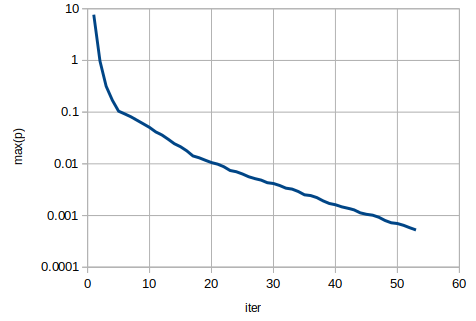
\includegraphics[width=0.6\linewidth]{linear2_simple_pres.png}
\end{center}


\subsubsection{Течение Пуазейля}
TODO

\subsubsection{Стационарное обтекание квадратного препятствия}

В тесте \ename{obstacle2-simple} из файла \ename{obstacle_simple_test.cpp}
рассматривается задача о стационарном обтекании
квадтратного препятствия (см. постановку в п. \ref{sec:problem-obstacle}).
По окончании расчёта в консоль печатаются коэффициенты сопротивления и подъёмной силы.

Используется естественная нумерация узлов с неактивными ячейками.
Класс \cvar{RegularGrid2D} предлагает следующие методы, связанные с неактивными ячейками:
\begin{itemize}
\item
\cvar{void RegularGrid2D::deactivate_cells(Point bot_left, Point top_right)} -- установить область неактивных ячеек;
\item
\cvar{bool RegularGrid2D::is_active_cell(size_t icell)} -- проверить, является ли ячейка активной.
\end{itemize}

Кроме того, в задаче появились внутренние границы.
То есть для постаноки граничных условий уже не достаточно
использовать крайние значение индексов $i$, $j$,
а нужен механизм для получения граничных отрезков сетки.
Для этого введены следующие функции
\begin{itemize}
\item
\cvar{RegularGrid2d::boundary_yfaces()} -- получить список всех вертикальных граничных фасок (возвращает парные индексы в
соответствии \cvar{yface_centered_grid}.
\item
\cvar{RegularGrid2d::boundary_xfaces()}  -- получить список всех горизонтальных граничных фасок (возвращает парные индексы в
соответствии \cvar{xface_centered_grid}.
\item
\cvar{RegularGrid2d::yface_type(size_t yface_index)} -- узнать тип вертикальной грани по её глобальному индексу.
Возвращает перечисление
\begin{minted}[linenos=false]{c++}
enum struct FaceType{
	Internal,     // внутренняя
	Boundary,     // граничная
	Deactivated   // неактивная (находится внутри неактивной области)
};
\end{minted}
\item
\cvar{RegularGrid2d::xface_type(size_t xface_index)} -- узнать тип вертикальной грани по её глобальному индексу.
\end{itemize}

\subsubsubsection{Функция верхнего уровня}
\clisting{open}{"test/obstacle_simple_test.cpp"}
\clisting{pass}{"TEST_CASE"}
Здесь сначала происходит установка параметров расчёта: числа Рейнольдса, параметра $E$,
количества итераций, порога сходимости и разбиения единичного интервала.
\clisting{lines-range}{"double Re", "n_unit"}
Далее строится сетка
\clisting{line}{"grid"}
В этом примере сетка строится в четырёхугольнике $[0, 12]\times[-2,2]$.
Потом для описания квадтратного препятствия 
происходит деактивация ячеек, находящихся в единичном квадрате
с нижней левой координатой $(2, -0.5)$ и верхней правой координатой $(3, 0.5)$.
\clisting{line}{"deactivate_cells"}
Потом создаётся решатель, инициализируются функции сохранения
и вызывается алгоритм потенциальной инициализации расчётных полей.
\clisting{until}{"worker.initialize();"}

Затем идёт стандартный цикл по SIMPLE-итерациям 
\clisting{block}{"size_t it = 0;"}

По окочании цикла вызывается функция сохранения решения в vtk
\clisting{line}{"worker.save_current_fields(it);"}

В конце происходит расчёт коэффициентов сил и их печать в консоль
\clisting{lines-range}{"coefs", "Cx"}
Результирующее поле течения сохраняется в файл \ename{obstacle2.vtk.series}.

\subsubsubsection{Учёт неактивных ячеек}
\clisting{to-start}{}
Неактивные ячейки учитываются во всех алгоритмах
сборки систем линейных уравнений. Рассмотрим на примере сборки
матрицы для пробной скорости, реализованной в функции \cvar{assemble_u_slae}.
\clisting{line}{"void Obstacle2DSimpleWorker::assemble_u_slae()"}
\clisting{pass}{"// internal"}
Рассмотрим цикл сборки внутренних узлов ``красной'' сетки для $u$
(или, что тоже самое, цикл по всем вертикальным граням основной сетки)
\clisting{lines-range}{"size_t j", "size_t i"}
Сначала вычисляется индекс строки (сквозной индекс текущей грани):
\clisting{line}{"row_index"}
Эта грань может быть либо внутренней, либо граничной (принадлежать внутренней вертикальной границе),
либо неактивной.
Выполняется проверка, является ли эта грань внутренней
\clisting{line}{"FaceType::Internal"}
Если да, то выполняется обычная процедура сборки
\clisting{before}{"else"}
Если нет (то есть грань либо неактивная, либо принадлежит внутренней границе),
то в диагональ ставится единица, в правую часть 0.
\clisting{block}{"else"}
Это отражает тот факт, что на внутренних границах $u=0$ из-за условий прилипания,
а для неактивных мы пишем тривиальное уравнение, просто чтобы матрица не была вырождена.

\clisting{to-start}{}
\clisting{pass}{"void Obstacle2DSimpleWorker::assemble_u_slae()"}
Учёт условий прилипания на внутренних горизонтальных
границах осуществляется через фиктивный узел в лямбда-функции \cvar{"add_to_mat"},
которая перехватывает все ситуации, когда алгоритм требует добавить что-либо в фиктивную колонку матрицы.
\clisting{line}{"auto add_to_mat"}
Такие ситуации могут произойти либо при сборке
около вертикальной грани, находящейся рядом с верхней границей:
\clisting{lines-range}{"if (ij_col[1] == _grid.ny())", "add_value"}
либо около вертикальной грани, находящейся рядом с нижней границей границей:
\clisting{lines-range}{"if (ij_col[1] == (size_t)-1)", "add_value"}
либо около вертикальнй грани, находящейся непосредственно над или под препятствием.
В этом случае индекс фиктивной колонки, в которую трубуется поставить будет
соответствовать неакотвной вертикальной грани.
Мы вычисляем этот индекс
\clisting{before}{"if"}
Если он неактивный, то следуем по процедуре добавления фиктивного узла около
границы с нулевым значением.
\clisting{block}{"if"}
Иначе -- это нормальная колонка и мы добавляем туда значение по стандартной процедуре
\clisting{line}{"add_value"}

\subsubsubsection{Расчёт коэффициентов сопротивления}
\label{sec:prog-cxcy}
\clisting{to-start}{}
Расчёт коэффициентов сил по формулам \cref{eq:ns2d_cx} осуществляется в процедуре \cvar{coefficients()}.
Она возвращает структуру, куда входят все шесть искомых значений
\clisting{block}{"struct Coefficients"}
Процедура, объявленная как
\clisting{line}{"Obstacle2DSimpleWorker::coefficients()"}
производит вычисления четырёх интегралов по простой квадратуре
\cref{eq:ns2d_gamma_quadrature}.
Результаты аггрегируются в переменные
\clisting{lines-range}{"sum_cpx", "sum_cfx"}
Операции проводятся в циклах по внутренним граничным отрезкам.
Сначала рассматриваются вертикальные границы:
\clisting{line}{"for (const RegularGrid2D::split_index_t& yface: _grid.boundary_yfaces())"}
Здесь в переменную \cvar{yface} попадают все парные индексы вертикальных граней, лежащих
на границах. Сначала нужно отфильтровать границы, лежащие во входном и выходном сечениях
\clisting{until}{" else "}
На вертикальных границах актуально вычисление коэффициентов $C^p_x$ (из пункта \ref{sec:compute-obstacle-coefs}).
Дли их определения на каждой сеточной грани мы должны определить
$p\,n_x$ по формулах \cref{eq:ns2d_obstacle_pnx_vertical}.
\clisting{line}{"pnx"}
Для использования этих формул нужно определить, является ли это левой или правой границей обтекаемого тела.
Мы вычисляем индексы ячеек, лежащих слева и справа.
Если левая ячейка активна, значит это левая граница, если правая активна, значит это правая граница.
\clisting{until}{"right_cell"}
Далее левой границы
\clisting{lines-range}{"if", "pnx"}
для правой
\clisting{lines-range}{"if", "pnx"}
иначе (если это и не правая и не левая граница) бросается исключение,
потому что так быть не должно: у любой внутренней границы должна быть хоть одна соседняя активная ячейка
\clisting{block}{"else"}
После вычисления $p\,n_x$ они добавляются
в искомые интегралы согласно
\cref{eq:ns2d_gamma_quadrature}:
\clisting{line}{"sum_cpx"}

Далее аналогичная процедура проводится для горизонтальных граней,
где актуально вычисление коэффициентов $C^f_x$.
Дли их определения на каждой сеточной грани мы должны определить
$\dsfr{u}{n}$ по формулах \cref{eq:ns2d_dudn_upper,eq:ns2d_dudn_lower}.

\clisting{block}{"for (const RegularGrid2D::split_index_t& xface: _grid.boundary_xfaces())"}

В конце функции искомые коэффициенты вычисляются через
уже найденные интегралы согласно
\cref{eq:ns2d_cx}:
\clisting{lines-range}{"Coefficients", "return"}

\subsubsubsection{Результаты расчёта}
Картина течения, полученная для
сетки \cvar{n_part = 10} при $\Ren = 20$,
представлена на \figref{fig:obstacle2-flow}
\begin{figure}[h!]
\centering
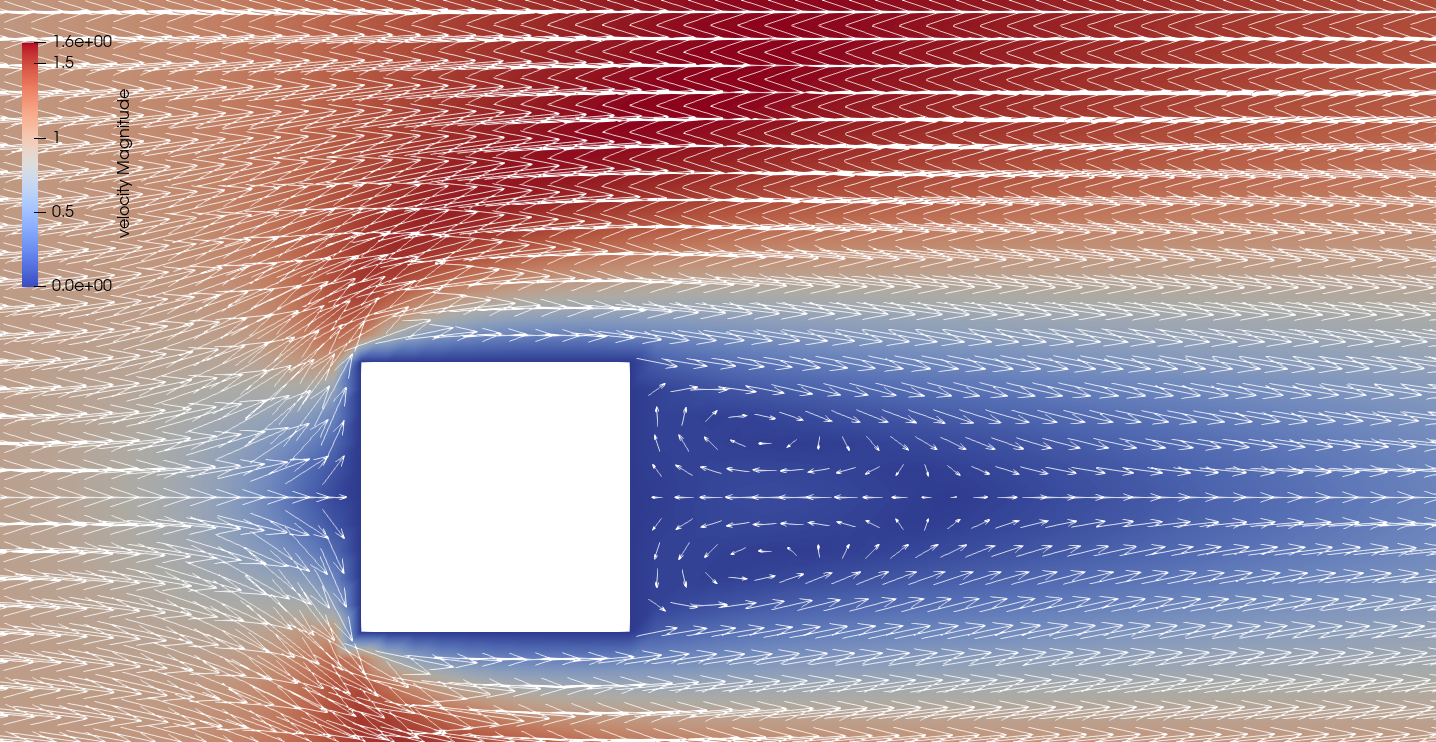
\includegraphics[width=0.9\linewidth]{obstacle2-flow.png}
\caption{Обтекание квадратного препятствия в стационарном режиме}
\label{fig:obstacle2-flow}
\end{figure}
Полученные коэффициенты сопротивления:
\begin{shelloutput}
=== Drag
Cpx = 2.97224
Cfx = 1.08639
Cx  = 4.05863
\end{shelloutput}
Для $\eps = 10^{-1}$ решение сошлось за 29 итераций.

\subsubsection{Нестационарное обтекание квадратного препятствия}
\label{sec:prob-obstacle-temp}

Эта задача реализована в файле \ename{obstacle_nonstat_simple_test.cpp}
в тесте \ename{[obstacle2-nonstat-simple]}.

Программа решает задачу в той же области, которая рассматривалась
в предыдущем пункте, но в нестационарной постановке
\cref{eq:ns2d_nonstat}

Поля течения для разных моментов времени пишутся в файл
\ename{obstacle-nonstat.vtk.series}. Кроме того, в файл \ename{c.txt}
пишутся вычисленные на разные моменты времени коэффициенты сопротивления.

\subsubsubsection{Функция верхнего уровня}
\clisting{open}{"test/obstacle_nonstat_simple_test.cpp"}
В начале обозначим параметры задачи:
числа Рейнольдса,
разбиение единичного отрезка,
шаг по времени $\dt$ и конечное время, 
параметр внутреннего итерационного процесса $E$, 
максимальное количество итераций во внутреннем итерационном процессе
и порог по невязке:
\clisting{pass}{"TEST_CASE"}
\clisting{lines-range}{"Re", "eps"}

Далее проводится создание сетки (так же, как и в предыдущем примере) и начальная инициализация
решателя
\clisting{lines-range}{"grid", "save_current_fields"}

После всех инициализаций начинается цикл по времени
\clisting{line}{"for (double time=time_step; time<end_time+1e-6; time+=time_step)"}
Отметим, что поскольку значению $t=0$ соответствует начальное
состояние решения, то цикл начинается сразу с первого шага $t=\dt$.

Внутри цикла по времени производится цикл
внутренних итераций SIMPLE
\clisting{block}{"size_t it"}

Далее, если текущее время кратно $1.0$, производится сохранение
решения в файл vtk и запись коэффициентов сил в файл:
\clisting{block}{"if"}

Печатается информация о сходимости текущей итерации
\clisting{line}{"cout"}

и производится переход на следующий шаг по времени:
\clisting{line}{"to_next_time_step"}

\subsubsubsection{Учёт нестационарности}
Согласно пунку \ref{sec:ns2d-nonstat} наличие производной по времени
учитывается:
\begin{itemize}
\item
При вычислении коэффициентов $d^u$, $d^v$
\cref{eq:ns2d_nonstat_duv}:
\clisting{to-start}{}
\clisting{pass}{"ObstacleNonstat2DSimpleWorker::ObstacleNonstat2DSimpleWorker("}
\clisting{lines-range}{"_du", "_dv"}
\item
При сборке систем уравнений для $u^*$, $u^*$
\cref{eq:ns2d_nonstat_uvstar}
\clisting{to-start}{}
\clisting{pass}{"void ObstacleNonstat2DSimpleWorker::assemble_u_slae()"}
как прибавка к диагонали
\clisting{line}{"add_to_mat(row_index, {i, j}, 1.0 + _tau/_time_step)"}
и правой части
\clisting{line}{"_rhs_u[row_index] += (_tau/_time_step)*_u_old[row_index]"}
\item
А так же в граничных условиях на выходе.
В этом случае условия \cref{eq:ns2d_outflow_common}
для $u$ по аналогии с \cref{eq:ns2d_outflow_common_semi}
аппроксимируются к виду
\begin{equation*}
(x,y)\in\Gamma_{out}:\; \frac{\hat u - \check u}{\dt} + \frac{\hat u - u}{\tau} + u\dfr{\hat u}{x} = 0.
\end{equation*}
Для упрощения по прежнему будем использовать ``стационарное'' условие
для поперечной скорости $v=0$.
Тогда для $u^*$ можно записать
$$
(x,y)\in\Gamma_{out}:\;
	\left(1 + \frac{\tau}{\dt}\right)u^*_{n_x, j+\tfrac12}
	+ \tau U_{n_x, j+\tfrac12}\frac{u^*_{n_x, j+\tfrac12}
					- u^*_{n_x-1, j+\tfrac12}}{h_x}
	= u_{n_x, j+\tfrac12}
	+ \frac\tau\dt \check u_{n_x, j+\tfrac12}
$$
Это выражение и добавляется в соответствующие строки матрицы и правой части
\clisting{to-start}{}
\clisting{pass}{"void ObstacleNonstat2DSimpleWorker::assemble_u_slae()"}
\clisting{block}{"// right boundary: du/dt + u*du/dx = 0"}
\item
При переходе на слудующий шаг по времени в функции
\clisting{to-start}{}
происходит вычисление текущего значения температуры, и
присваивание значений $\check u$, $\check v$.
\clisting{block}{"double ObstacleNonstat2DSimpleWorker::to_next_time_step()"}
Вызов \cvar{set_uvp} здесь осуществляется для пересборки актуальных матриц.

\end{itemize}

\subsection{Задание для самостоятельной работы}
\subsubsection{Расчитать коэффициент подъёмной силы}
Добавить расчёт коэффициентов подъёмной силы $C_y$ в
код для моделирования нестационарного обтекания (\ref{sec:prob-obstacle-temp}).
В п.(\ref{sec:prog-cxcy}) представлен используемый алгоритм
расчёта коэффицента сопротивления.
Отталкиваясь от этого алгоритма необходимо
\begin{itemize}
\item в класс \cvar{Coefficients} добавить поля \cvar{Cpy,Cfy,Cy},
\item добавить расчёт \cvar{dvdn} на вертикальных стенках препятствия по формулам  \cref{eq:ns2d_obstacle_dvdn_vertical},
\item добавить расчёт \cvar{pny} на горизонтальных стенках препятствия по формулам \cref{eq:ns2d_obstacle_pny_top,eq:ns2d_obstacle_pny_bot},
\item аггрегировать эти значения в \cvar{sum_cpy,sum_cfy}, из которых вычислить коэффициенты подъёмной силы,
\item сами коэффициенты добавить в файл \ename{c.txt}.
\end{itemize}


\subsubsection{Расчёт течения}
Провести расчёт течения при параметрах $\Ren = 100$, $\eps=10^{-1}$, $\dt = 0.1$, $t_{end} = 200$, $n=10$.
(для ускорения расчётов не забыть переключиться на релизную сборку).
\begin{itemize}
\item Показать динамику изменения расчётных полей: скалярных $p$, $|\vec v|$ и вектора скорости $\vec v$,
\item Нарисовать графики изменения коэффициентов сопротивления $C_x, C^p_x, C^f_x$ и подъёмной силы $C_y, C^p_y, C^f_y$ во времени.
\end{itemize}


\appendix
\section{Формулы и обозначения}
\subsection{Векторы}

\subsubsection{Обозначение}

Геометрические вектора обозначаются жирным шрифтом $\vec v$.
Скалярные координаты вектора -- через нижний индекс с обозначением
оси координат: $\left(v_x, v_y, v_z\right)$.
Если вектор $\vec u$ -- вектор скорости, то его декартовые координаты
имеют специальное обозначение $\vec u = \left(u, v, w\right)$.
Единичные вектора, соответствующие осям координат, обозначаются 
знаком $\hat\cdot$: $\vec{\hat x}$, $\vec{\hat y}$, $\vec{\hat z}$.
Координатные векторы обозначаются по символу первой оси. Например, $\vec x = (x, y, z)$ или $\vec \xi = (\xi, \eta, \zeta)$.

Операции в векторами имеют следующее обозначение (расписывая в декартовых координатах):
\begin{itemize}
\item
Умножение на скалярную функцию
\begin{equation}
\label{eq:vec_scalar}
f \vec u = (f u_x)\vec{\hat x} + (f u_y)\vec{\hat y} + (f u_z)\vec{\hat z};
\end{equation}
\item
Скалярное произведение
\begin{equation}
\label{eq:vec_dot}
\vec u \cdot \vec v = u_x v_x + u_y v_y + u_z v_z;
\end{equation}
\item
Векторное произведение
\begin{equation}
\label{eq:vec_cross}
\vec u\times\vec v = 
\left|
\begin{array}{ccc}
\vec{\hat x} & \vec{\hat y} & \vec{\hat z} \\
u_x & u_y & u_z \\
v_x & v_y & v_z
\end{array}
\right| = 
\left(u_y v_z - u_z v_y\right)\vec{\hat x} -
\left(u_x v_z - u_z v_x\right)\vec{\hat y} +
\left(u_x v_y - u_y v_x\right)\vec{\hat z}.
\end{equation}

\end{itemize}

В двумерном случае можно считать, что $u_z = v_z = 0$.
Тогда результатом векторного произведения согласно \cref{eq:vec_cross} 
будет вектор, направленный перпендикулярно плоскости $xy$:
$$
\vec u \times \vec v = (u_x v_y - u_y v_x)\vec{\hat z}.
$$
При работе с двумерными задачами, где ось $\vec z$ отсутствует,
обычно результатом векторного произведения считают скаляр
\begin{equation}
\label{eq:vec_cross_2d}
2D: \; \vec u \times \vec v = u_x v_y - u_y v_x.
\end{equation}
Геометрический смысл этого скаляра: площадь
параллелограмма, построенного на векторах $\vec u$ и $\vec v$.


\subsubsection{Набла--нотация}

Символ $\nabla$ -- есть псевдовектор, который выражает
покоординатные производные.
Для декартовой системы координат $(x, y, z)$ он запишется в виде
$$
\nabla = \left( \dfr{}{x}, \; \dfr{}{y}, \; \dfr{}{z} \right).
$$
В радиальной $(r, \phi, z)$:
$$
\nabla = \left( \dfr{}{r}, \; \frac{1}{r}\dfr{}{\phi}, \; \dfr{}{z} \right).
$$
В цилиндрической $(r, \theta, \phi)$:
$$
\nabla = \left( \dfr{}{r}, \; \frac{1}{r}\dfr{}{\theta}, \; \frac{1}{r\sin\theta}\dfr{}{\phi} \right).
$$
Удобство записи дифференциальных выражений с использованием $\nabla$ заключается в независимости записи от
вида системы координат.
Но если требуется обозначить производную по конкретной координате,
то, по аналогии с обычными векторами, это делается через нижний индекс:
$$
\nabla_n f = \dfr{f}{n}.
$$

Для этого символа справедливы все векторные операции, описанные ранее.
Так, применение $\nabla$ к скалярной функции аналогично умножению вектора
на скаляр \cref{eq:vec_scalar} (здесь и далее приводятся покоординатные выражения для декартовой системы):
\begin{equation}
\label{eq:del_grad}
\nabla f  = \left(\nabla_x f, \; \nabla_y f, \; \nabla_z f\right) = \dfr{f}{x}\vec{\hat x} + \dfr{f}{y}\vec{\hat y} + \dfr{f}{z}\vec{\hat z}.
\end{equation}
Результатом этой операции является вектор.

Скалярное умножение $\nabla$ на вектор $\vec v$ по аналогии с \cref{eq:vec_dot} -- есть дивергенция:
\begin{equation}
\label{eq:del_div}
\nabla \cdot \vec v  = \dfr{v_x}{x} + \dfr{v_y}{y} + \dfr{v_z}{z}
\end{equation}
результат которой -- скалярная функция.

Двойное применение $\nabla$ к скалярной функции -- это оператор Лапласа:
\begin{equation}
\label{eq:del_laplace}
\nabla \cdot \nabla f  = \nabla^2 f = \dfrq{f}{x} + \dfrq{f}{y} + \dfrq{f}{z}
\end{equation}

Ротор -- аналог векторного умножнения \cref{eq:vec_cross}:
\begin{equation}
\label{eq:del_rotor}
\nabla\times\vec v = 
\left|
\begin{array}{ccc}
\vec{\hat x} & \vec{\hat y} & \vec{\hat z} \\
\nabla_x & \nabla_y & \nabla_z \\
v_x & v_y & v_z
\end{array}
\right| = 
\left(\dfr{v_z}{y} - \dfr{v_y}{z}\right)\vec{\hat x} -
\left(\dfr{v_z}{x} - \dfr{v_x}{z}\right)\vec{\hat y} +
\left(\dfr{v_y}{x} - \dfr{v_x}{y}\right)\vec{\hat z}.
\end{equation}

\subsection{Интегрирование}
\label{sec:partint} 

\subsubsection{Формула Гаусса--Остроградского}

Формула Гаусса--Остроградского, связывающая
интегрирование по объёму $E$ с интегрированием по границе этого объёма $\Gamma$,
для векторного поля $\vec v$ имеет вид
\begin{equation}
\label{eq:partint_div}
\arint{\nabla\cdot\vec v}{E}{\vec x} = \arint{v_n}{\Gamma}{s},
\end{equation}
где $\vec n$ -- внешняя по отношению к области $E$ нормаль.
Смысл этой формулы можно проиллюстрировать на одномерном примере.
Пусть одномерное векторное поле $v_x = f(x)$ на отрезке $E = [a, b]$ задано
функцией, представленной на \figref{fig:div1d}.
\begin{figure}[h!]
\centering
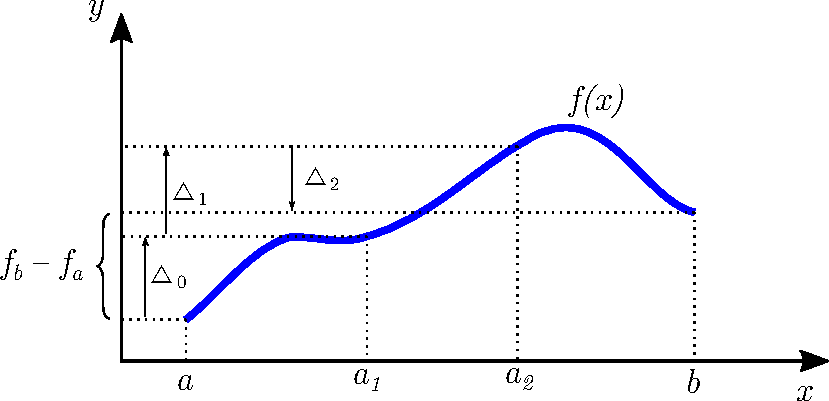
\includegraphics[width=0.6\linewidth]{div1d.pdf}
\caption{Формула Гаусса-Остроградского в одномерном случае}
\label{fig:div1d}
\end{figure}
Разобъем область на $N=3$ равномерных подобласти длины $h$. Тогда
расписывая интеграл как сумму, а производную через конечную разность, получим
$$
\arint{\dfr{f}{x}}{E}{x} \approx \sum_{i=0}^{2} h \left(\dfr{f}{x}\right)_{i+\tfrac12}
\approx\sum_{i=0}^{2}(f_{i+1} - f_{i})
= \triangle_0 + \triangle_1 + \triangle_2 = f_b - f_a.
$$
Очевидно что, при устремлении $N\to\infty$ правая часть предыдущего выражения не изменится.
То есть, сумма всех изменений функции в области есть изменение функции по её границам:
$$
\int\limits_{a}^{b}\dfr{f}{x}\,dx = f(b) - f(a).
$$
А формула \cref{eq:partint_div} -- есть многомерное обобщение этого выражения.

\subsubsection{Интегрирование по частям}

Подставив в \cref{eq:partint_div} $\vec v = f\vec u$, где $f$ -- некоторая скалярная функция, и 
расписав дивергенцию в виде
$$\nabla\cdot(f\vec u) = f\nabla\vec u + \vec u \cdot \nabla f$$
получим формулу интегрирования по частям
\begin{equation}
\label{eq:partint}
\arint{\vec u \cdot \nabla f}{E}{\vec x} = \arint{f u_n}{\Gamma}{s} - \arint{f\nabla\cdot \vec u}{E}{\vec x}
\end{equation}
Распишем некоторые частные случаи для формулы \cref{eq:partint}.
Для $\vec u = (n_x, 0, 0)$ получим
\begin{equation}
\label{eq:partint_ugrad_}
\arint{\dfr{f}{x}}{E}{\vec x} = \arint{f \cos(\vecangle{n}{x})}{\Gamma}{s}
\end{equation}
При $\vec u = \nabla g$
\begin{equation}
\label{eq:partint_laplace_fg}
\arint{f\left(\nabla^2 g \right)}{E}{\vec x} = \arint{f\dfr{g}{n}}{\Gamma}{s} - \arint{\nabla f \cdot \nabla g}{E}{\vec x}
\end{equation}
При $f=1$ и $\vec u = \nabla g$
\begin{equation}
\label{eq:partint_laplace}
\arint{\nabla^2 g}{E}{\vec x} = \arint{\dfr{g}{n}}{\Gamma}{s}
\end{equation}

\subsubsection{Численное интегрирование в заданной области}
Квадратурная формула
\begin{equation}
\label{eq:quadrature_formula}
\arint{f(\vec x)}{E}{\vec x} = \sum_{i=0}^{N-1} w_i f(\vec x_i)
\end{equation}
Она определяется заданием узлов интегрирования $\vec x_i$ 
и соответствующих весов $w_i$.

\subsection{Интерполяционные полиномы}

\subsubsection{Многочлен Лагранжа}

\subsubsubsection{Узловые базисные функции}

Рассмотрим функцию $f(\xi)$, заданную в области $D$.
Внутри этой области зададим $N$ узловых
точек $\xi_i, i=\overline{0,N-1}$.
Приближение функции $f$ будем искать в виде
\begin{equation}
\label{eq:nodal_basis}
f(\xi) \approx \sum_{i=0}^{N-1} f_i \phi_i(\xi),
\end{equation}
где  $f_i = f(\xi_i)$, $\phi_i$ -- узловая базисная функция.
Потребуем, чтобы это выражение выполнялось точно для всех
заданных узлов интерполяции $\xi = \xi_i$. Тогда, исходя из определения \cref{eq:nodal_basis}, запишем условие 
на узловую базисную функцию
\begin{equation}
\label{eq:nodal_bases_conditions}
\phi_i(\xi_j) = 
\begin{cases}
1, &\quad i = j, \\
0, &\quad i \neq j.
\end{cases}
\end{equation}
Дополнительно потребуем, чтобы формула \cref{eq:nodal_basis} была
точной для постоянных функций
$$
f(\xi)=\const \hence f_i = \const.
$$
Тогда для любого $\xi$ должно выполняться условие
\begin{equation}
\label{eq:nodal_bases_unitsum}
\sum_{i=0}^{N-1} \phi_i(\xi) = 1, \qquad \xi \in D.
\end{equation}

Задача построения интерполяционной функции состоит
в конкретном определении узловых базисов
$\phi_i(\xi)$ по заданному набору
узловых точек $\xi_i$ и значениям
функции в них $f_i$. Будем искать базисы
в виде многочленов вида
\begin{equation}
\label{eq:nodal_basis_1d_decomp}
\phi_i(\xi) = \sum_{a} A_i^{(a)} \xi^{a} =
A_i^{(0)} + 
A_i^{(1)} \xi + 
A_i^{(2)} \xi^2 +  \ldots, \qquad i = \overline{0, N-1}.
\end{equation}
Определять коэффициенты $A^{(a)}_i$ будем из условий \cref{eq:nodal_bases_conditions},
которое даёт $N$ линейных уравнений относительно неизвестных $A_i^{(a)}$ для каждого $i=\overline{0, N-1}$.
Таким образом, в выражениях \cref{eq:nodal_basis_1d_decomp} должно быть
ровно $N$ слагаемых.
Будем использовать последовательный набор степеней: $a=\overline{0,N-1}$.
Выпишем систему линейных уравнений для $0$-ой базисной функции
\begin{equation*}
\begin{aligned}
& \phi_0(\xi_0) = A_0^{(0)} + A_0^{(1)} \xi_0 + A_0^{(2)} \xi_0^2 + A_0^{(3)} \xi_0^3 + \ldots = 1, \\
& \phi_0(\xi_1) = A_0^{(0)} + A_0^{(1)} \xi_1 + A_0^{(2)} \xi_1^2 + A_0^{(3)} \xi_1^3 + \ldots = 0, \\
& \phi_0(\xi_2) = A_0^{(0)} + A_0^{(1)} \xi_2 + A_0^{(2)} \xi_2^2 + A_0^{(3)} \xi_2^3 + \ldots = 0, \\
& \ldots
\end{aligned}
\end{equation*}
или в матричном виде
\begin{equation*}
\left(
\begin{array}{ccccc}
1 & \xi_0 & \xi_0^2 & \xi_0^3 & \ldots \\[5pt]
1 & \xi_1 & \xi_1^2 & \xi_1^3 & \ldots \\[5pt]
1 & \xi_2 & \xi_2^2 & \xi_2^3 & \ldots \\[5pt]
1 & \xi_3 & \xi_3^2 & \xi_3^3 & \ldots \\[5pt]
\ldots &&&&
\end{array}
\right)
\left(
\begin{array}{c}
A_0^{(0)} \\[5pt]
A_0^{(1)} \\[5pt]
A_0^{(2)} \\[5pt]
A_0^{(3)} \\[5pt]
\vdots
\end{array}
\right)
=
\left(
\begin{array}{c}
1 \\[5pt]
0 \\[5pt]
0 \\[5pt]
0 \\[5pt]
\vdots
\end{array}
\right)
\end{equation*}
Записывая аналогичные выражения для остальных базисных функций, получим систему матричных уравнений
вида $C A = E$:
\begin{equation*}
\left(
\begin{array}{ccccc}
1 & \xi_0 & \xi_0^2 & \xi_0^3 & \ldots \\[5pt]
1 & \xi_1 & \xi_1^2 & \xi_1^3 & \ldots \\[5pt]
1 & \xi_2 & \xi_2^2 & \xi_2^3 & \ldots \\[5pt]
1 & \xi_3 & \xi_3^2 & \xi_3^3 & \ldots \\[5pt]
\ldots &&&&
\end{array}
\right)
\left(
\begin{array}{ccccc}
A_0^{(0)} & A_1^{(0)} & A_2^{(0)} & A_3^{(0)} & \ldots\\[5pt]
A_0^{(1)} & A_1^{(1)} & A_2^{(1)} & A_3^{(1)} &       \\[5pt]
A_0^{(2)} & A_1^{(2)} & A_2^{(2)} & A_3^{(2)} &       \\[5pt]
A_0^{(3)} & A_1^{(3)} & A_2^{(3)} & A_3^{(3)} &       \\[5pt]
\vdots
\end{array}
\right)
=
\left(
\begin{array}{ccccc}
1 & 0 & 0 & 0 & \ldots \\[5pt]
0 & 1 & 0 & 0 &        \\[5pt]
0 & 0 & 1 & 0 &        \\[5pt]
0 & 0 & 0 & 1 &        \\[5pt]
\vdots
\end{array}
\right)
\end{equation*}
Отсюда матрица неизвестных коэффициентов $A$ определится как
\begin{equation}
\label{eq:nodal_basic_amat}
A = C^{-1} = 
\left(
\begin{array}{ccccc}
1 & \xi_0 & \xi_0^2 & \xi_0^3 & \ldots \\[5pt]
1 & \xi_1 & \xi_1^2 & \xi_1^3 & \ldots \\[5pt]
1 & \xi_2 & \xi_2^2 & \xi_2^3 & \ldots \\[5pt]
1 & \xi_3 & \xi_3^2 & \xi_3^3 & \ldots \\[5pt]
\ldots &&&&
\end{array}
\right) ^{-1}.
\end{equation}

Подставляя полином \cref{eq:nodal_basis_1d_decomp} в условие согласованности \cref{eq:nodal_bases_unitsum},
получим требование
\begin{equation*}
\sum_{i=0}^{N-1} A_i^{(a)} = 
\begin{cases}
1, \quad a=0, \\
0, \quad a=\overline{1,N-1}.
\end{cases}
\end{equation*} 
То есть сумма всех свободных членов в интерполяционных полиномах должна
быть равна единице, а сумма коэффициентов при остальных степенях -- нулю.
Можно показать, что это свойство выполняется для любой матрицы $A=C^{-1}$,
в случае, если первый столбец матрицы $C$ состоит из единиц.
То есть условие согласованности требует наличие свободного члена
с интерполяционном полиноме.


\subsubsubsection{Интерполяция в параметрическом отрезке}
\label{sec:segment_bases}
Будем рассматривать область интерполяции $D=[-1, 1]$.
В качестве первых двух узлов интерполяции возьмем границы области:
$\xi_0 = -1$, $\xi_1 = 1$.
\paragraph{Линейный базис}
Будем искать интерполяционный базис в виде
$$
\phi_i(\xi) = A_i^{(0)} + A_i^{(1)} \xi.
$$
на основе двух условий:
$$
\phi_i(-1) = A_i^{(0)} - A_i^{(1)} = \delta_{0i}, \quad \phi_i(1) = A_i^{(0)} + A_i^{(1)}\delta_{1i}.
$$
Составим матрицу $C$, записав эти условия в матричном виде
$$
C =
\left(
\begin{array}{l|rr}
      & A^{(0)} & A^{(1)}\\
\hline
\phi(-1) & 1 & -1 \\[5pt]
\phi(1) & 1 &  1 \\[5pt]
\end{array}
\right)
$$
и, согласно \cref{eq:nodal_basic_amat}, найдём матрицу коэффициентов
$$
A =
\left(
\begin{array}{cc}
A_0^{(0)} & A_1^{(0)} \\[5pt]
A_0^{(1)} & A_1^{(1)} \\[5pt]
\end{array}
\right) = C^{-1} =
\left(
\begin{array}{l|rr}
     & \phi_0   & \phi_1  \\
\hline
1    & \frac12  & \frac12 \\[5pt]
\xi  & -\frac12 & \frac12 \\[5pt]
\end{array}
\right).
$$
Отсюда узловые базисные функции примут вид (\figref{fig:basis1d_linear})
\begin{equation}
\label{eq:segment_linear_basis}
\begin{aligned}
&\phi_0(\xi) = \frac{1 - \xi}{2}, \\
&\phi_1(\xi) = \frac{1 + \xi}{2}.
\end{aligned}
\end{equation}
Окончательно интерполяционная функция из определения \cref{eq:nodal_basis}
примет вид
$$
f(\xi) \approx \frac{1 - \xi}{2} f(-1) + \frac{1 + \xi}{2} f(1).
$$
\begin{figure}[h!]
\centering
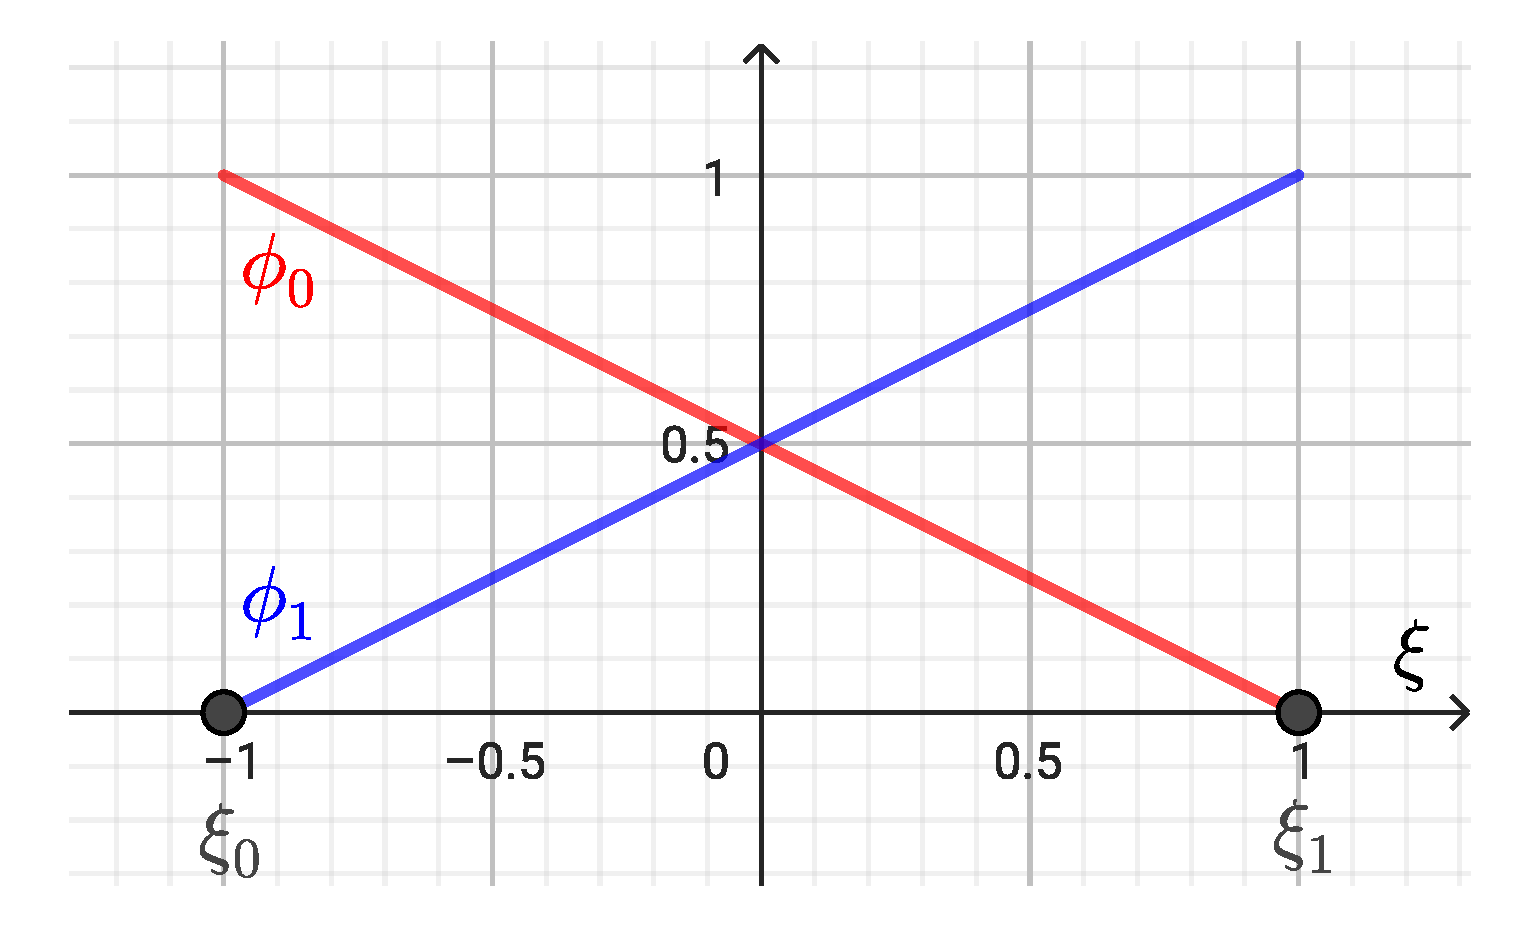
\includegraphics[width=0.4\linewidth]{basis1d_linear.pdf}
\caption{Линейный базис в параметрическом отрезке}
\label{fig:basis1d_linear}
\end{figure}

\paragraph{Квадратичный базис}
Будем искать интерполяционный базис в виде
$$
\phi_i(\xi) = A_i^{(0)} + A_i^{(1)} \xi + A_i^{(2)} \xi^2.
$$
По сравнению с линейным случаем, в форму базиса добавился ещё один неизвестый коэффициент $A_i^{(2)}$,
поэтому в набор условий \cref{eq:nodal_bases_conditions} требуется ещё одно уравнение (ещё одна узловая точка).
Поместим её в центр параметрического сегмента $\xi_2 = 0$. Далее будем действовать по
аналогии с линейным случаем:
$$
C = \left(
\begin{array}{l|rrr}
         &  A^{(0)} & A^{(1)}   & A^{(2)} \\ 
\hline
\phi(-1) & 1 & -1 & 1\\[5pt]
\phi(1)  & 1 &  1 & 1\\[5pt]
\phi(0)  & 1 &  0 & 0
\end{array}
\right)
\hence
A = C^{-1} = \left(
\begin{array}{l|rrr}
       & \phi_0   & \phi_1   & \phi_2 \\
\hline
 1     & 0        &  0       &  1     \\[5pt]
 \xi   & -\frac12 &  \frac12 &  0     \\[5pt]
 \xi^2 &  \frac12 &  \frac12 & -1     \\[5pt]
\end{array}
\right).
$$
Узловые базисные функции для квадратичной интерполяции примут вид (\figref{fig:basis1d_quadratic})
\begin{equation}
\label{eq:segment_quadratic_basis}
\begin{aligned}
&\phi_0(\xi) = \frac{\xi^2 - \xi}{2}, \\
&\phi_1(\xi) = \frac{\xi^2 + \xi}{2}, \\
&\phi_2(\xi) = 1 - \xi^2.
\end{aligned}
\end{equation}

\begin{figure}[h!]
\centering
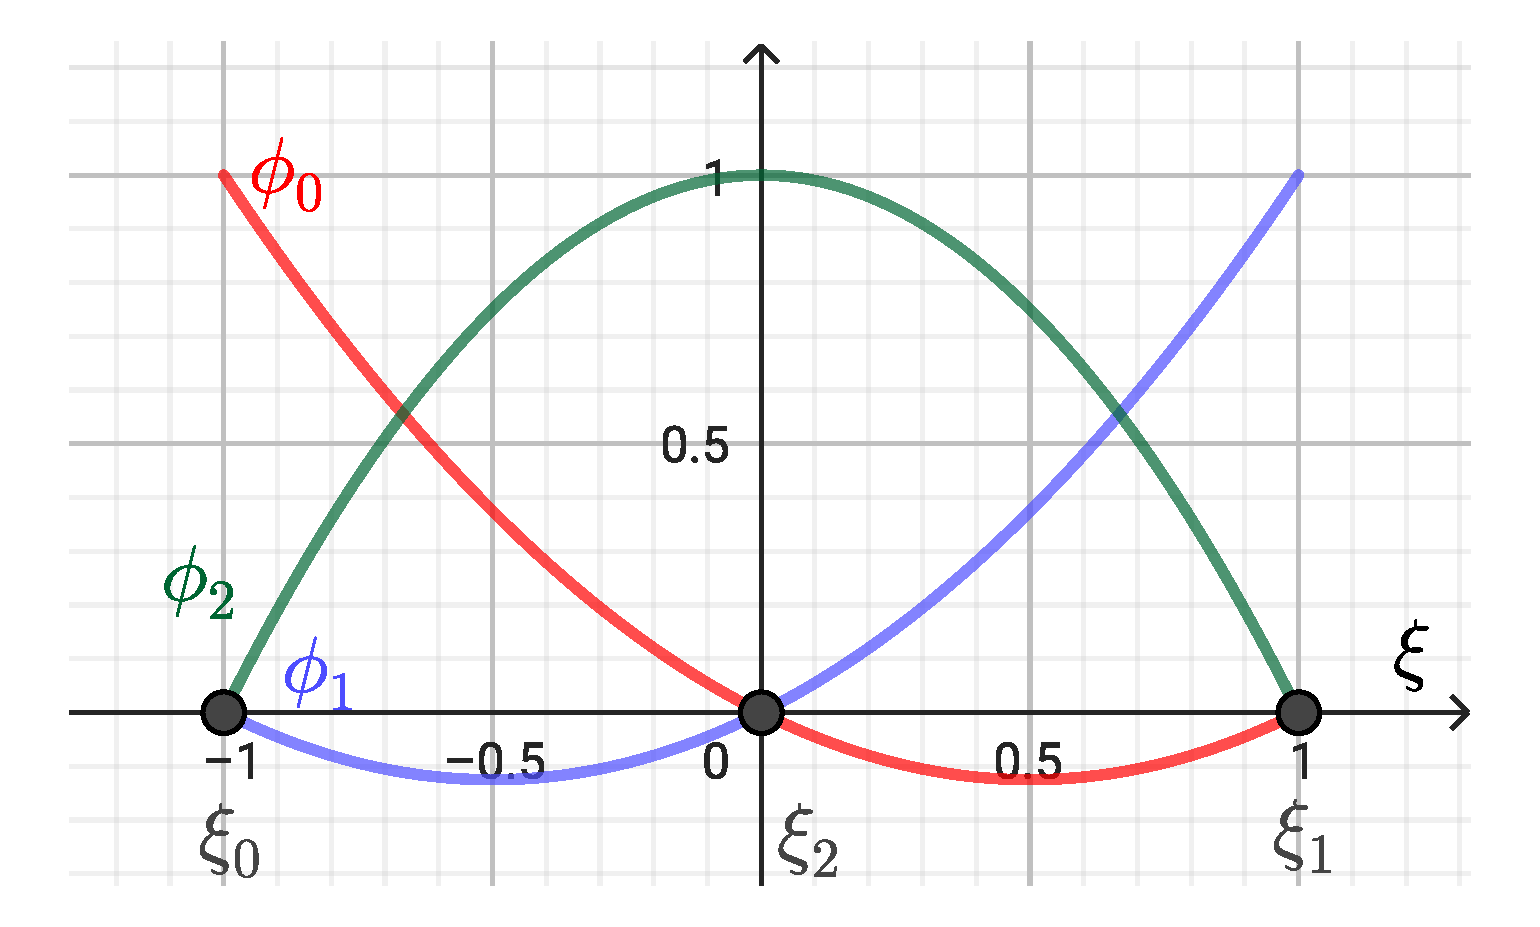
\includegraphics[width=0.4\linewidth]{basis1d_quadratic.pdf}
\caption{Квадратичный базис в параметрическом отрезке}
\label{fig:basis1d_quadratic}
\end{figure}

\paragraph{Кубический базис}
Интерполяционный базис будет иметь вид
$$
\phi_i(\xi) = A_i^{(0)} + A_i^{(1)} \xi + A_i^{(2)} \xi^2 + A_i^{(3)} \xi^3.
$$
Для нахождения четырёх коэффициентов нам понадобится четыре узла интерполяции.
Две из них -- это границы параметрического отрезка. Остальные две разместим
так, чтобы разбить отрезок на равные интервалы:
$\xi_2 = -\tfrac13$, $\xi_3 = \tfrac13$.
Далее вычислим матрицу коэффициентов:
$$
C =
\left(
\begin{array}{l|rrrr}
                &  A^{(0)}  &  A^{(1)}      & A^{(2)}     & A^{(3)}         \\
\hline
\phi(-1)        &  1  & -1        & 1         &  -1           \\[5pt]
\phi( 1)        &  1  & 1         & 1         &   1           \\[5pt]
\phi(-\tfrac13) &  1  & -\tfrac13 & \tfrac19  &  -\tfrac1{27} \\[5pt]
\phi(\tfrac13)  &  1  &  \tfrac13 & \tfrac19  &   \tfrac1{27}
\end{array}
\right)
\hence
A = C^{-1} =
\frac{1}{16}
\left(
\begin{array}{l|rrrr}
      & \phi_0 & \phi_1 & \phi_2 & \phi_3 \\
\hline
1     & -1     & -1     &   9    &  9     \\[5pt]
\xi   &  1     & -1     & -27    &  27    \\[5pt]
\xi^2 &  9     &  9     & -9     & -9     \\[5pt]
\xi^3 & -9     &  9     &  27    & -27   
\end{array}
\right)
$$
Узловые базисные функции для квадратичной интерполяции примут вид (\figref{fig:basis1d_cubic})
\begin{equation}
\label{eq:segment_cubic_basis}
\begin{aligned}
&\phi_0(\xi) = \frac{1}{16}\left(-1 + \xi + 9 \xi^2 -9 \xi^3\right), \\
&\phi_1(\xi) = \frac{1}{16}\left(-1 - \xi + 9 \xi^2 +9 \xi^3\right), \\
&\phi_2(\xi) = \frac{1}{16}\left(9 -27 \xi - 9\xi^2 + 27 \xi^3\right), \\
&\phi_3(\xi) = \frac{1}{16}\left(9 +27 \xi - 9\xi^2 - 27 \xi^3\right), \\
\end{aligned}
\end{equation}

\begin{figure}[h!]
\centering
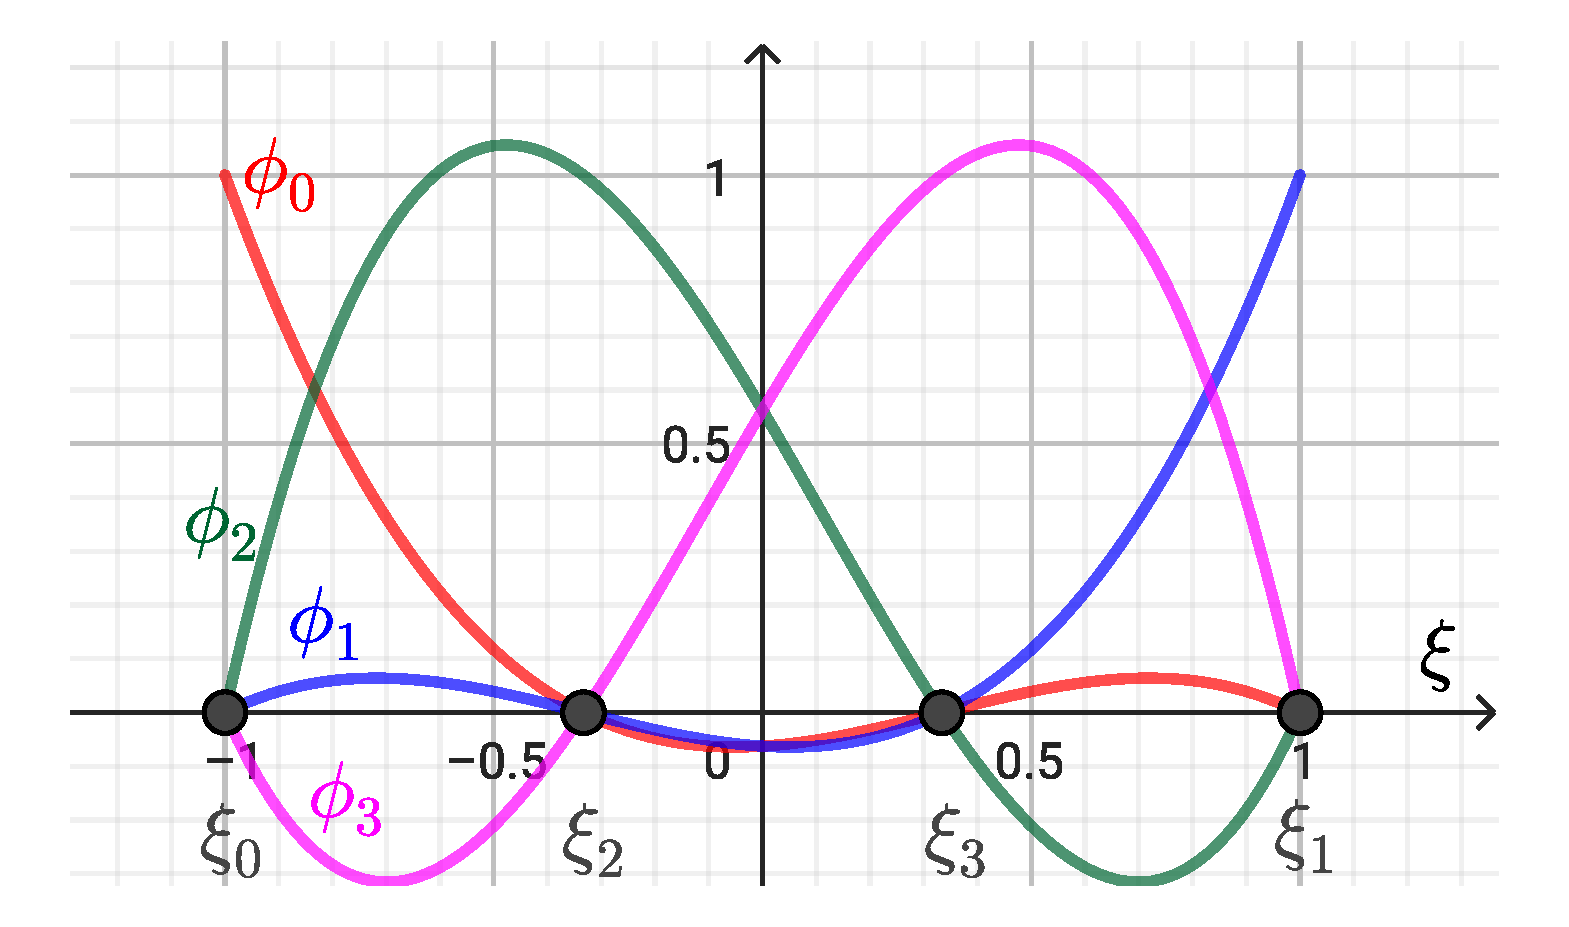
\includegraphics[width=0.4\linewidth]{basis1d_cubic.pdf}
\caption{Кубический базис в параметрическом отрезке}
\label{fig:basis1d_cubic}
\end{figure}

На \figref{fig:basis1d_compare} представлено сравнение результатов
аппроксимации функции $f(x) = -x + \sin(2 x + 1)$ линейным, квадратичным и кубическим базисом.
Видно, что все интерполяционные приближения точно попадают в функцию в своих
узлах интерполяции, а между узлами происходит аппроксимация полиномом соответствующей степени.

\begin{figure}[h!]
\centering
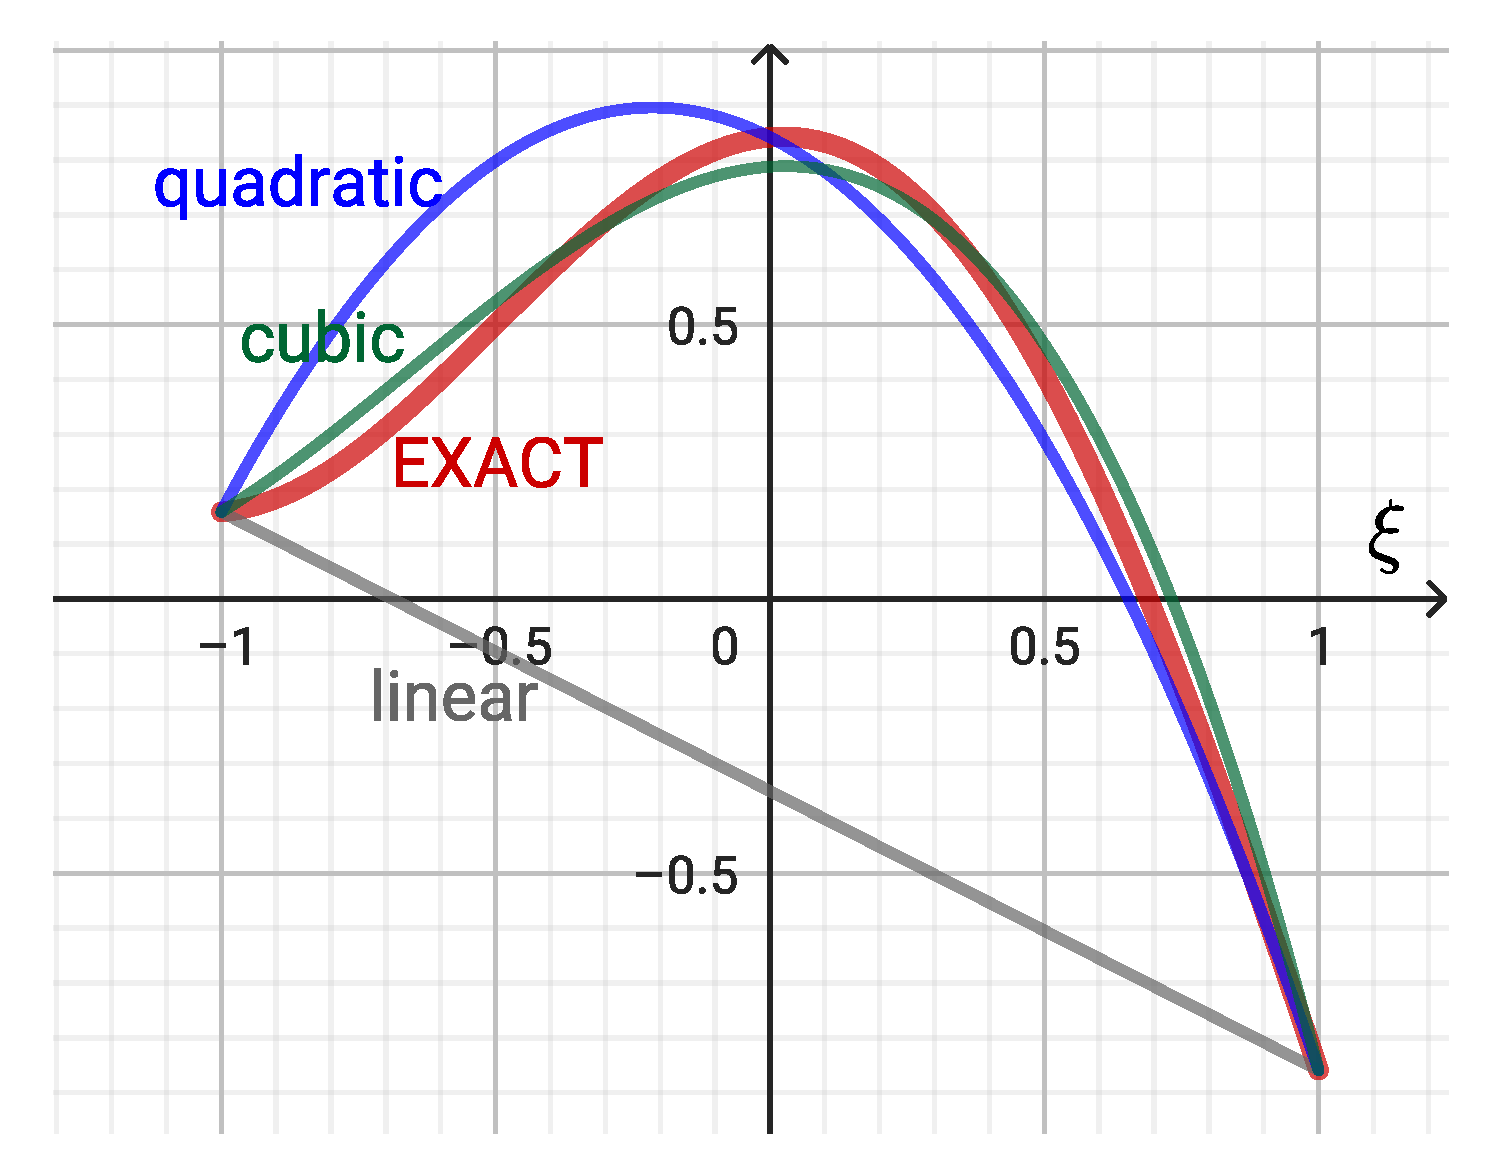
\includegraphics[width=0.4\linewidth]{basis1d_compare.pdf}
\caption{Результат интерполяции}
\label{fig:basis1d_compare}
\end{figure}

\subsubsubsection{Интерполяция в параметрическом треугольнике}
\label{sec:triangle_bases}
Теперь рассмотрим двумерное обобщение формулы
\begin{figure}[h!]
\centering
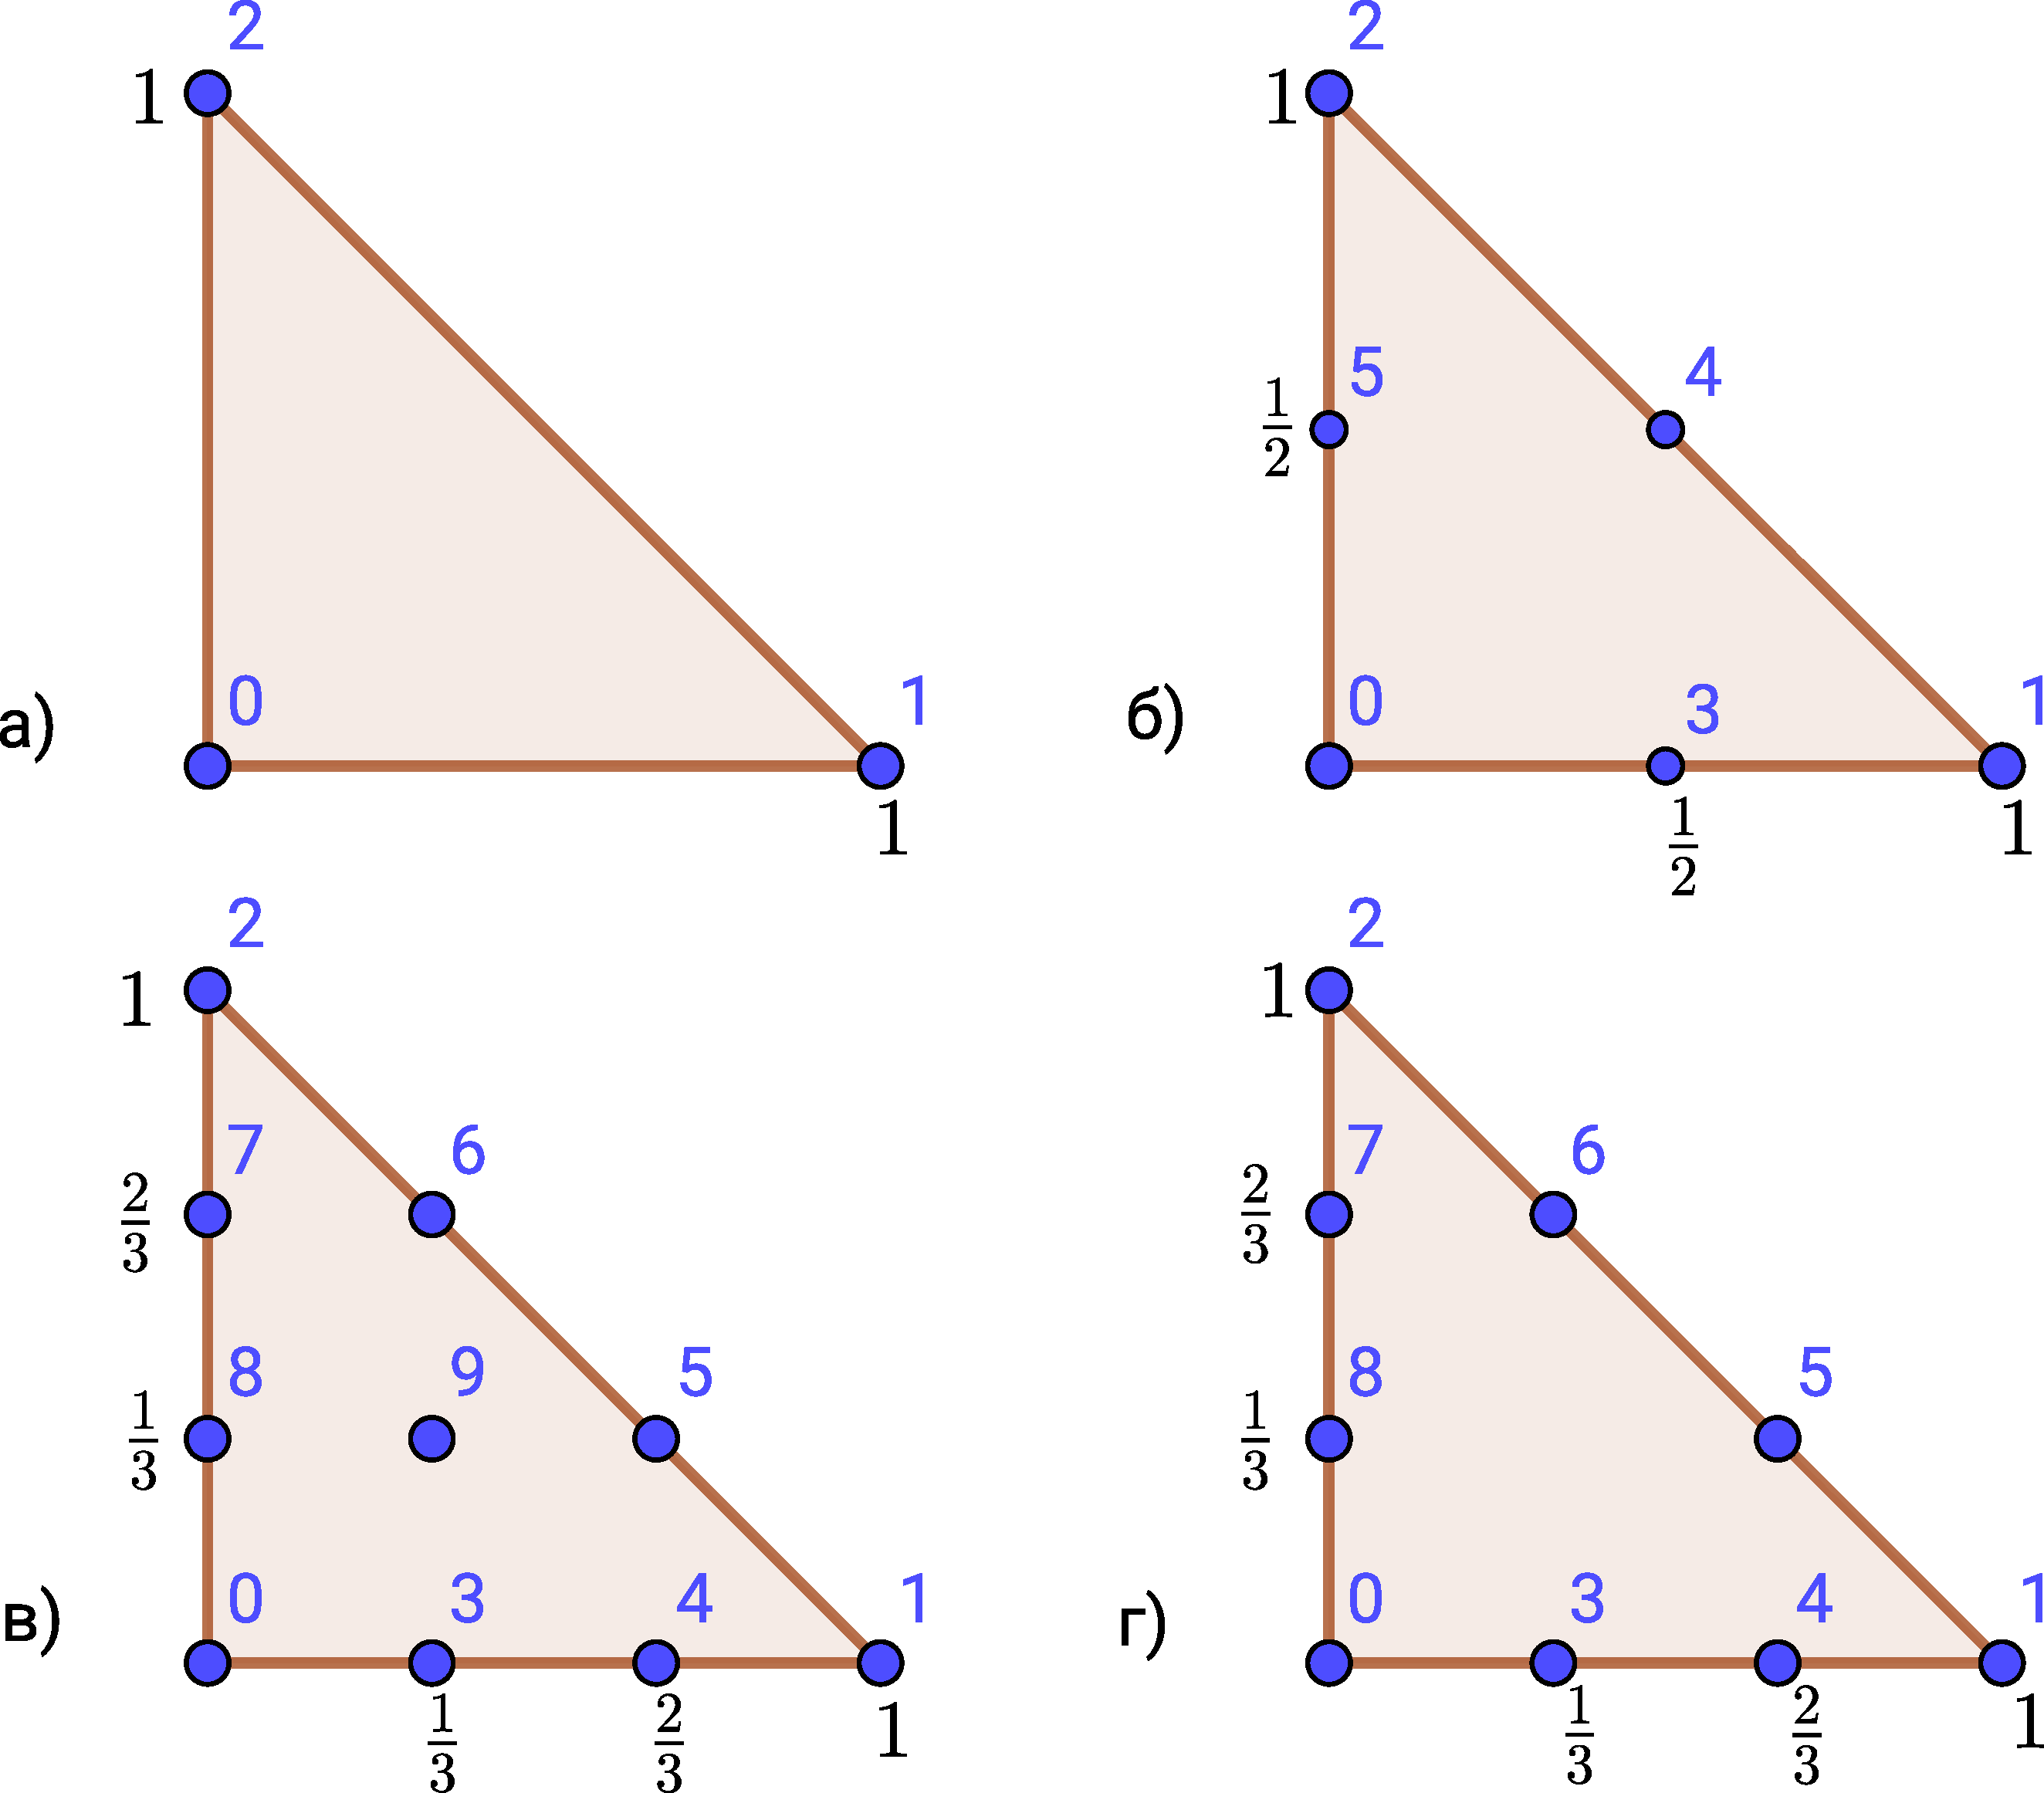
\includegraphics[width=0.5\linewidth]{triangle_basis_points.pdf}
\caption{Расположение узловых точек в параметрическом треугольнике. а) линейный базис, б) квадратичный базис, в) кубический базис, г) неполный кубический базис}
\label{fig:triangle_basis_points}
\end{figure}
\paragraph{Линейный базис}

\begin{equation*}
\phi_i(\xi, \eta) = A_i^{(00)} + A_i^{(10)} \xi + A_i^{(01)} \eta.
\end{equation*}
\begin{equation*}
C = \left(
\begin{array}{l|ccc}
                  & A^{(00)}   & A^{(10)} & A^{(01)} \\
\hline
\phi(0, 0) & 1   & 0   & 0    \\[5pt]
\phi(1, 0) & 1   & 1   & 0    \\[5pt]
\phi(0, 1) & 1   & 0   & 1
\end{array}
\right)
\hence
A = C^{-1} = 
\left(
\begin{array}{l|rrr}
     & \phi_0 & \phi_1 & \phi_2 \\
\hline
1    & 1      & 0      & 0      \\[5pt]
\xi  &-1      & 1      & 0      \\[5pt]
\eta &-1      & 0      & 1
\end{array}
\right)
\end{equation*}

\begin{equation}
\label{eq:triangle_linear_basis}
\begin{aligned}
&\phi_0(\xi, \eta) = 1 - \xi - \eta, \\
&\phi_1(\xi, \eta) = \xi, \\
&\phi_2(\xi, \eta) = \eta, \\
\end{aligned}
\end{equation}

\begin{figure}[h!]
\centering
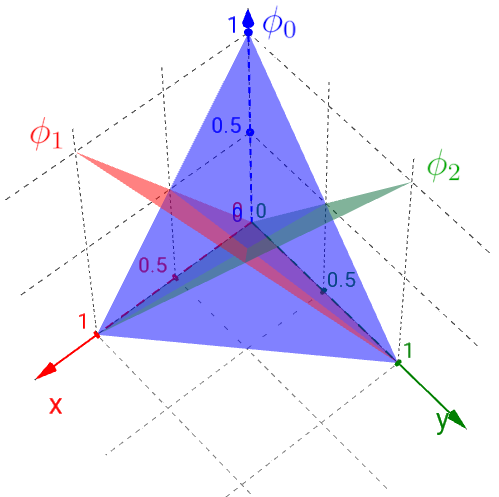
\includegraphics[width=0.4\linewidth]{basis2d_linear.png}
\caption{Линейный базис в параметрическом треугольнике}
\label{fig:basis2d_linear}
\end{figure}


\paragraph{Квадратичный базис}
\begin{equation*}
\phi_i(\xi, \eta) = A_i^{(00)} + A_i^{(10)} \xi + A_i^{(01)} \eta + A_i^{(11)} \xi \eta + A_i^{(20)} \xi^2 + A_i^{(02)} \eta^2.
\end{equation*}

\begin{equation*}
C =
\left(
\begin{array}{l|cccccc}
                     & A^{(00)} & A^{(10)}      & A^{(01)}  & A^{(11)}  & A^{(20)}    & A^{(02)}   \\[5pt]
\hline
\phi(0, 0)               & 1 &  0       &  0          &   0      &    0     &   0      \\[5pt]
\phi(1, 0)               & 1 &  1       &  0          &   0      &    1     &   0      \\[5pt]
\phi(0, 1)               & 1 &  0       &  1          &   0      &    0     &   1      \\[5pt]
\phi(\tfrac12, 0)        & 1 & \tfrac12 &  0          &   0      & \tfrac14 &   0      \\[5pt]
\phi(\tfrac12, \tfrac12) & 1 & \tfrac12 &  \tfrac12   & \tfrac14 & \tfrac14 & \tfrac14 \\[5pt]
\phi(0, \tfrac12)        & 1 &  0       &  \tfrac12   &   0      &    0     & \tfrac14 
\end{array}
\right)
\hence
A = \left(
\begin{array}{l|rrrrrr}
        & \phi_0 & \phi_1 & \phi_2 & \phi_3 & \phi_4 & \phi_5 \\[5pt]
\hline
1       & 1  &  0 & 0 & 0 & 0 & 0\\[5pt]
\xi     & -3 & -1 & 0 & 4 & 0 & 0\\[5pt]
\eta    & -3 & 0 & -1 & 0 & 0 & 4\\[5pt]
\xi\eta & 4 & 0 & 0 & -4 & 4 & -4\\[5pt]
\xi^2   & 2 & 2 & 0 & -4 & 0 & 0 \\[5pt]
\eta^2  & 2 & 0 & 2 & 0 & 0 & -4
\end{array}
\right)
\end{equation*}

\begin{figure}[h!]
\centering
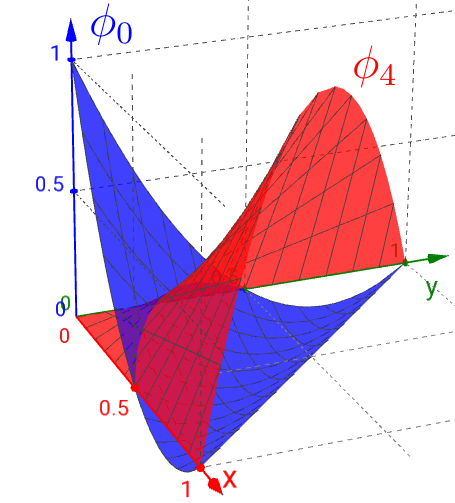
\includegraphics[width=0.3\linewidth]{basis2d_quadratic.png}
\caption{Квадратичные функции $\phi_0$, $\phi_4$ в параметрическом треугольнике}
\label{fig:basis2d_quadratic}
\end{figure}

\paragraph{Кубический базис}
TODO

\paragraph{Неполный кубический базис}
TODO

\subsubsubsection{Интерполяция в параметрическом квадрате}
\begin{figure}[h!]
\centering
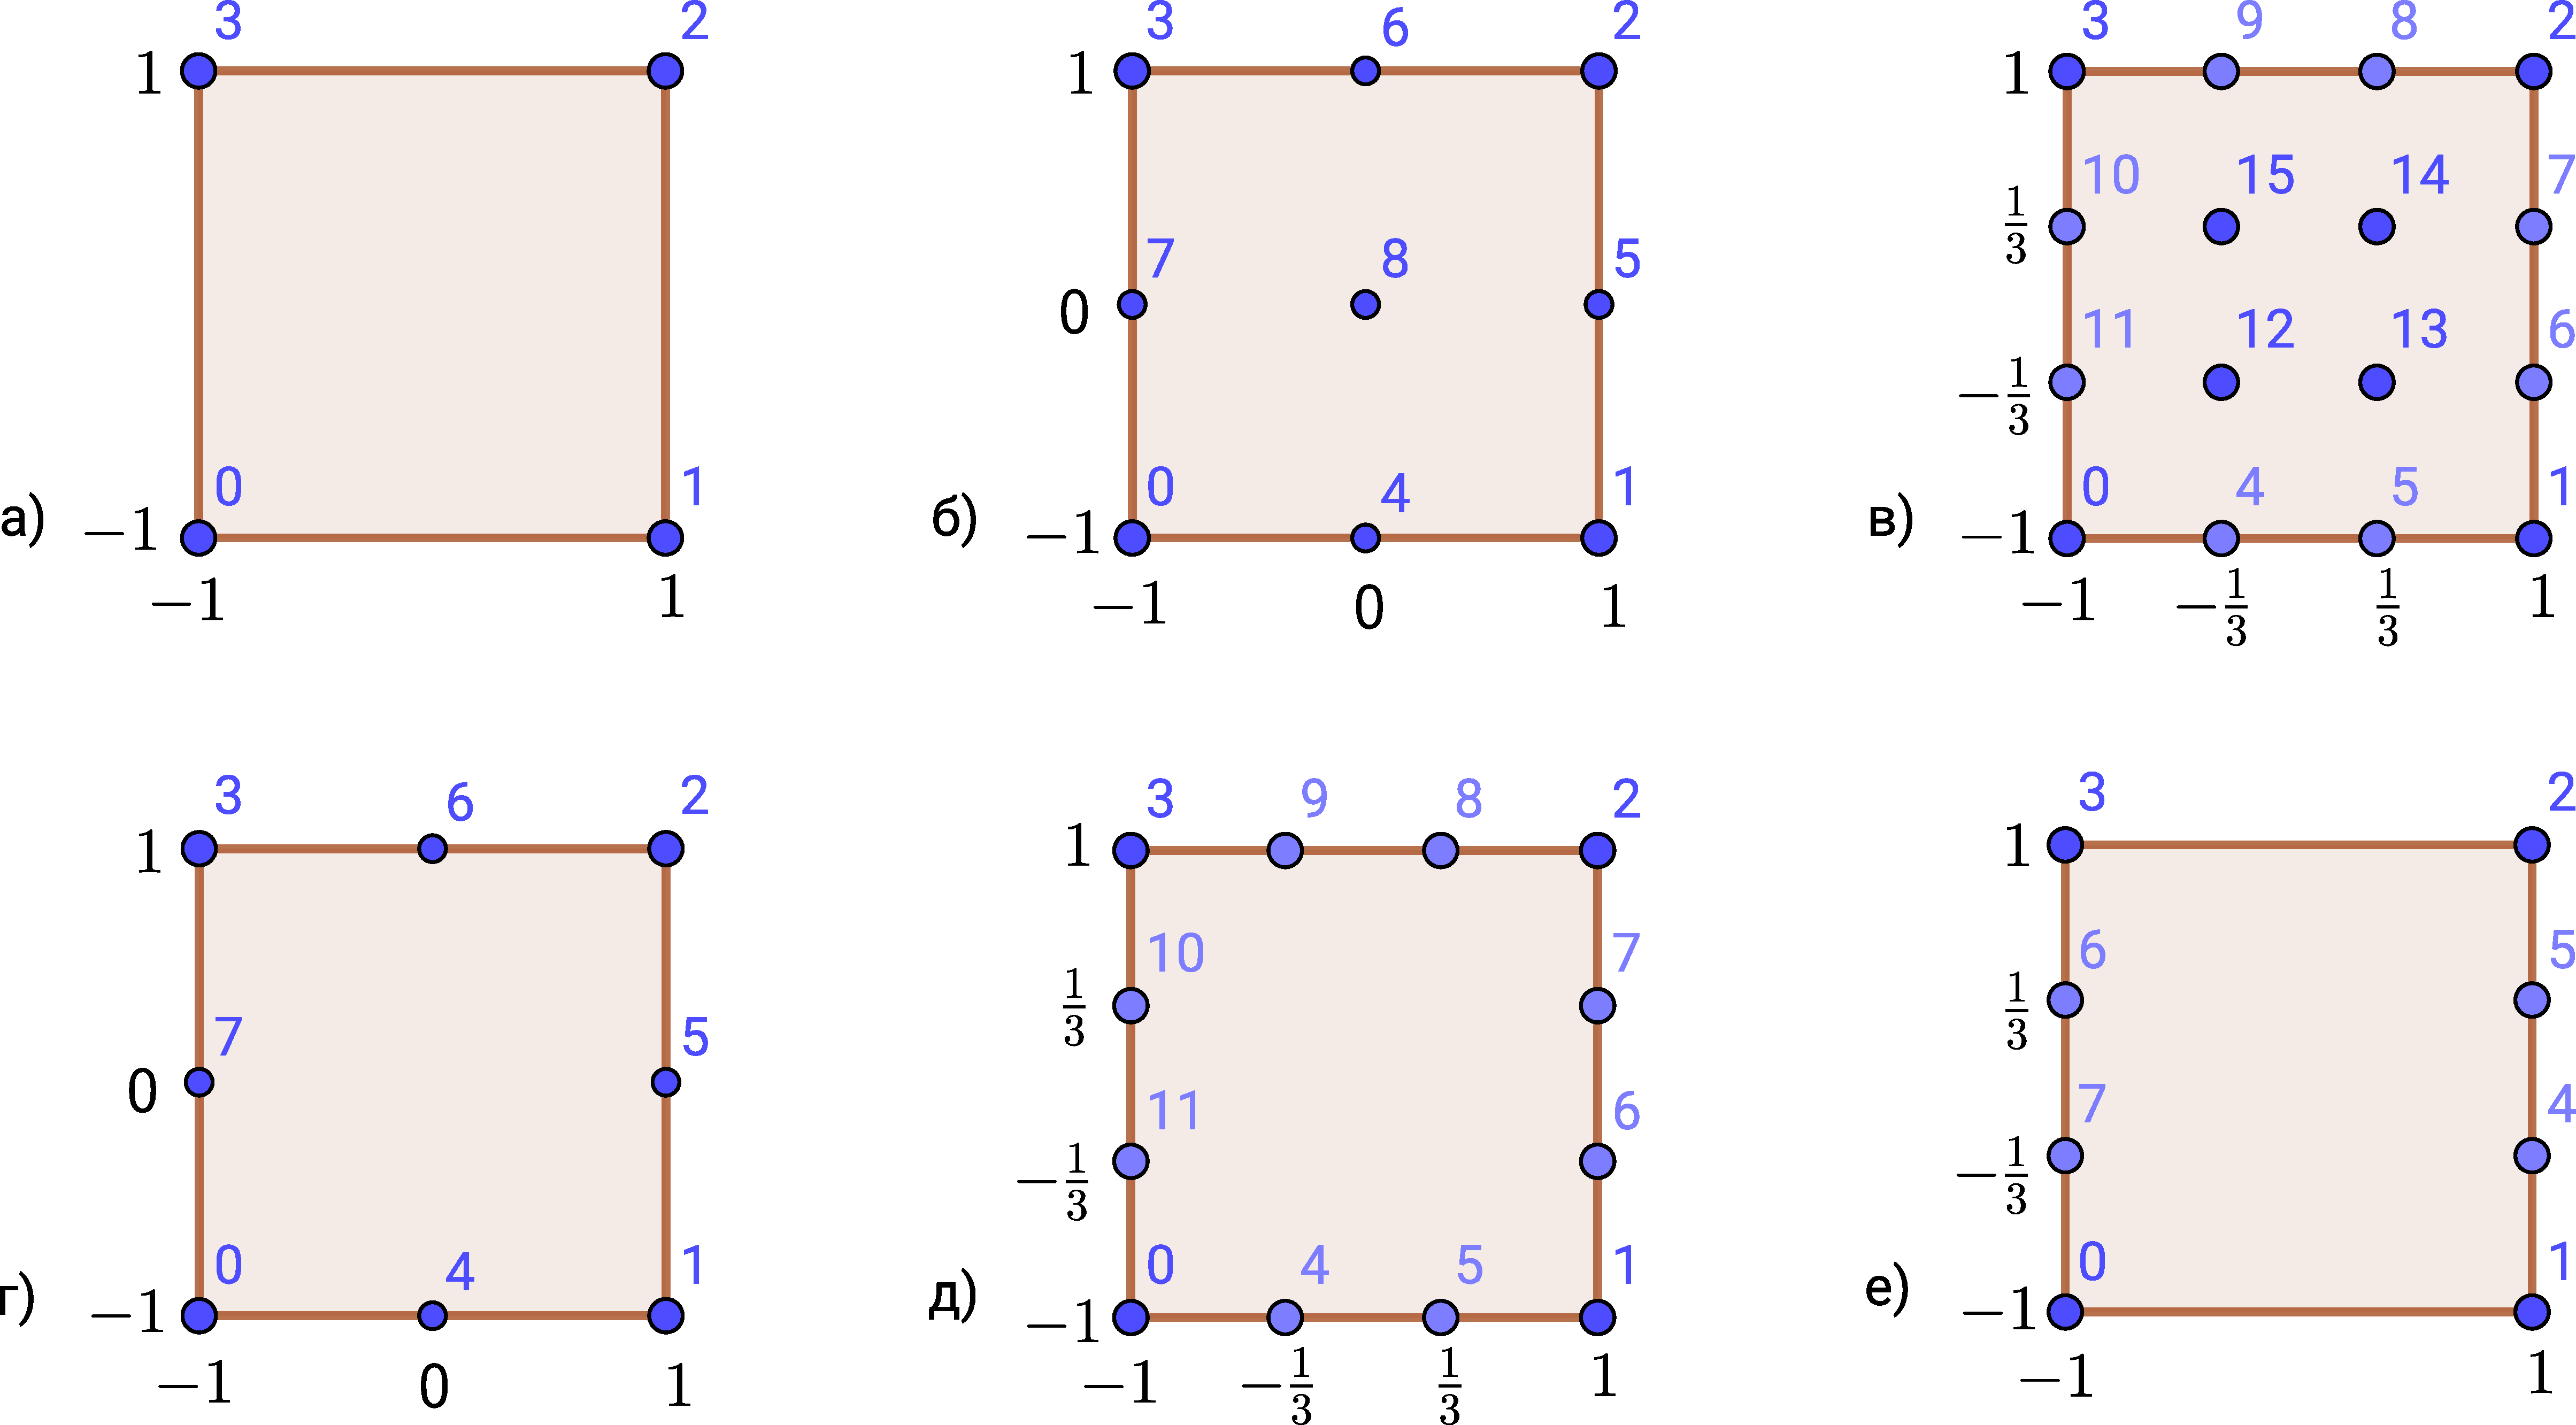
\includegraphics[width=0.7\linewidth]{quadrangle_basis_points.pdf}
\caption{Расположение узловых точек в параметрическом квадратре}
\label{fig:quadrangle_basis_points}
\end{figure}

\paragraph{Билинейный базис}
\begin{equation*}
\phi_i = A^{00}_i + A^{10}_i \xi + A^{01}_i \eta + A^{11}_i \xi\eta.
\end{equation*}

\begin{equation*}
C = \left(
\begin{array}{l|rrrr}
                      & A^{(00)} & A^{(10)} & A^{(01)} & A^{(11)} \\
\hline
\phi(-1, -1) & 1 & -1  & -1   &  1      \\[5pt] 
\phi( 1, -1) & 1 &  1  & -1   & -1      \\[5pt]
\phi( 1,  1) & 1 &  1  &  1   &  1      \\[5pt]
\phi(-1,  1) & 1 & -1  &  1   & -1      \\[5pt]
\end{array}
\right)
\hence
A = C^{-1} = \frac14\left(
\begin{array}{l|rrrr}
        & \phi_0 & \phi_1 & \phi_2 & \phi_3\\
\hline
1       & 1 & 1 & 1 & 1\\[5pt]
\xi     & -1 & 1 & 1 & -1\\[5pt]
\eta    & -1 & -1 & 1 & 1\\[5pt]
\xi\eta & 1 & -1 & 1 & -1
\end{array}
\right)
\end{equation*}

\begin{equation}
\label{eq:quadrangle_bilinear_basis}
\begin{aligned}
&\phi_0(\xi, \eta) = \frac{1-\xi-\eta+\xi\eta}{4}\\[10pt]
&\phi_1(\xi, \eta) = \frac{1+\xi-\eta-\xi\eta}{4}\\[10pt]
&\phi_2(\xi, \eta) = \frac{1+\xi+\eta+\xi\eta}{4}\\[10pt]
&\phi_3(\xi, \eta) = \frac{1-\xi+\eta-\xi\eta}{4}
\end{aligned}
\end{equation}

\begin{figure}[h!]
\centering
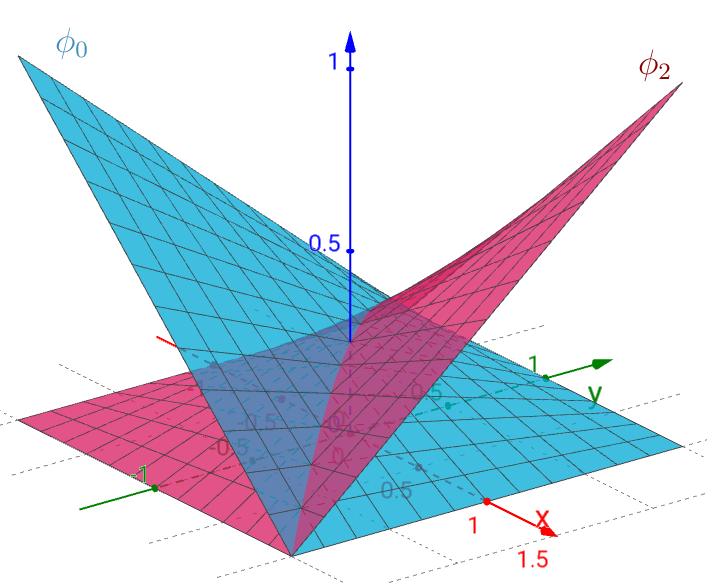
\includegraphics[width=0.4\linewidth]{basis2d_bilinear.png}
\caption{Билинейные функции $\phi_0$, $\phi_2$ в параметрическом квадрате}
\label{fig:basis2d_bilinear}
\end{figure}

\paragraph{Определение двумерных базисов через комбинацию одномерных}
Обратим внимание, что в искомые билинейные базисные функции линейны
в каждом из направлений $\xi, \eta$, если брать их по отдельности.
Значит можно представить эти функции как комбинацию одномерных
линейных базисов \cref{eq:segment_linear_basis} в каждом из направлений.
Узлы двумерного параметрического квадрата можно
выразить через узлы линейного базиса в параметрическом одномерном сегменте,
рассмотренном в п.~\ref{sec:segment_bases}:
$$
\vec \xi_0 = \left(\xi^{1D}_0, \xi^{1D}_0\right), \quad
\vec \xi_1 = \left(\xi^{1D}_1, \xi^{1D}_0\right), \quad
\vec \xi_2 = \left(\xi^{1D}_1, \xi^{1D}_1\right), \quad
\vec \xi_3 = \left(\xi^{1D}_0, \xi^{1D}_1\right).
$$
Значит и соответствующие базисные функции можно выразить
через линейный одномерный базис $\phi^{1D}$ из соотношений \cref{eq:segment_linear_basis}:
\begin{equation*}
\begin{aligned}
\phi_0(\xi, \eta) = \phi_0^{1D}(\xi)\phi^{1D}_0(\eta) = \frac{1-\xi}{2}\frac{1-\eta}{2},\\[5pt]
\phi_1(\xi, \eta) = \phi_1^{1D}(\xi)\phi^{1D}_0(\eta) = \frac{1+\xi}{2}\frac{1-\eta}{2},\\[5pt]
\phi_2(\xi, \eta) = \phi_1^{1D}(\xi)\phi^{1D}_1(\eta) = \frac{1+\xi}{2}\frac{1+\eta}{2},\\[5pt]
\phi_3(\xi, \eta) = \phi_0^{1D}(\xi)\phi^{1D}_1(\eta) = \frac{1-\xi}{2}\frac{1+\eta}{2}.
\end{aligned}
\end{equation*}
Раскрыв скобки можно убедится, что мы получили тот же билинейный базис, что и ранее \cref{eq:quadrangle_bilinear_basis}.

\paragraph{Биквадратичный базис}
Применим этот метод для вычисления биквадратичного базиса, определённого в точках на \figref{fig:quadrangle_basis_points}б.
В качестве основе возьмём квадратичный одномерный базис $\phi^{1D}_i$ из \cref{eq:segment_quadratic_basis}.
\begin{equation}
\label{eq:quadrangle_quadratic_basis}
\begin{array}{ll}
  \phi_0(\xi, \eta) = \phi_0^{1D}(\xi)\phi_0^{1D}(\eta) = \dfrac{\xi^2 - \xi}{2}\dfrac{\eta^2 - \eta}{2},
& \phi_1(\xi, \eta) = \phi_1^{1D}(\xi)\phi_0^{1D}(\eta) = \dfrac{\xi^2 + \xi}{2}\dfrac{\eta^2 - \eta}{2}, \\[10pt]
  \phi_2(\xi, \eta) = \phi_1^{1D}(\xi)\phi_1^{1D}(\eta) = \dfrac{\xi^2 + \xi}{2}\dfrac{\eta^2 + \eta}{2},
& \phi_3(\xi, \eta) = \phi_0^{1D}(\xi)\phi_1^{1D}(\eta) = \dfrac{\xi^2 - \xi}{2}\dfrac{\eta^2 + \eta}{2}, \\[10pt]
  \phi_4(\xi, \eta) = \phi_2^{1D}(\xi)\phi_0^{1D}(\eta) = (1-\xi^2)\dfrac{\eta^2 - \eta}{2},
& \phi_5(\xi, \eta) = \phi_1^{1D}(\xi)\phi_2^{1D}(\eta) = \dfrac{\xi^2 + \xi}{2}(1 - \eta^2),            \\[10pt]
  \phi_6(\xi, \eta) = \phi_2^{1D}(\xi)\phi_1^{1D}(\eta) = (1-\xi^2)\dfrac{\eta^2 + \eta}{2},
& \phi_7(\xi, \eta) = \phi_0^{1D}(\xi)\phi_2^{1D}(\eta) = \dfrac{\xi^2 - \xi}{2}(1 - \eta^2),            \\[10pt]
  \phi_8(\xi, \eta) = \phi_2^{1D}(\xi)\phi_2^{1D}(\eta) = (1-\xi^2)(1 - \eta^2).
&
\end{array}
\end{equation}

\paragraph{Бикубический базис}

\paragraph{Неполный биквадратичный базис}

\paragraph{Неполный бикубический базис}

\subsection{Геометрические алгоритмы}
\subsubsection{Линейная интерполяция}
\begin{figure}[h!]
\centering
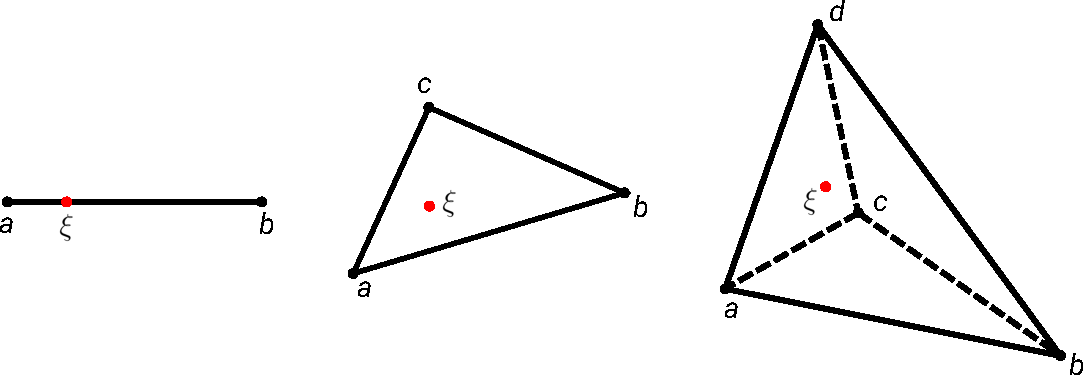
\includegraphics[width=0.8\linewidth]{geom_interp.pdf}
\caption{Порядок нумерации точек одномерного, двумерного и трёхмерного симплекса при линейной интерполяции}
\label{fig:geom_interp}
\end{figure}
Пусть функция $u$ задана в узлах симплекса, имеющего нумерацию согласно рис.~\ref{fig:geom_interp}.
Необходимо найти значение этой функции в точке $\vec \xi$ (эта точка вообще говоря не обязана лежать внутри симлекса).

Интерполяция в одномерном, двумерном и трёхмерном виде запишется как
\begin{align}
\label{eq:simplex_interp_1d}
&u(\xi) =
\frac{
|\triangle_{\xi a}|u(b)+
|\triangle_{b \xi}|u(a)
}
{|\triangle_{ba}|}
\\[10pt]
\label{eq:simplex_interp_2d}
&u(\xi) =
\frac{
|\triangle_{ab\xi}|u(c) +
|\triangle_{bc\xi}|u(a) +
|\triangle_{ca\xi}|u(b)
}
{|\triangle_{abc}|}
\\[10pt]
\label{eq:simplex_interp_3d}
&u(\xi) =
\frac{
|\triangle_{abc\xi}|u(d) +
|\triangle_{cbd\xi}|u(a) +
|\triangle_{cda\xi}|u(b) +
|\triangle_{adb\xi}|u(c)
}
{|\triangle_{abcd}|},
\end{align}
где $|\triangle|$ -- знаковый объём симплекса, вычисляемый как
\begin{align*}
& |\triangle_{ab}| = b - a, \\[10pt]
& |\triangle_{abc}| = \left(\frac{(\vec b - \vec a)\times(\vec c - \vec a)}{2}\right)_z, \\[10pt]
& |\triangle_{abcd}| = \frac{(\vec b - \vec a)\cdot\left((\vec c - \vec a)\times(\vec d - \vec a)\right)}{6}.\\[10pt]
\end{align*}

\subsubsection{Преобразование координат}
\label{sec:coo_transform} 
Рассмотрим преобразование
из двумерной параметрической системы координат $\vec \xi$ 
в физическую систему $\vec x$.
Такое преобразование полностью определяется покоординатными
функциями $\vec x(\vec \xi)$.
Далее получим соотношения, связывающие операции дифференцирования
и интегрирования в физической и параметрической областях.

\subsubsubsection{Матрица Якоби}
Будем рассматривать двумерное преобразование $(\xi, \eta) \to (x, y)$.
Линеаризуем это преобразование (разложим в ряд Фурье до линейного слагаемого)
\begin{align*}
& x(\xi_0 + d\xi, \eta_0 + d\eta) \approx x_0 + \left.\dfr{x}{\xi}\right|_{\xi_0, \eta_0} d\xi
    + \left.\dfr{x}{\eta}\right|_{\xi_0, \eta_0} d\eta, \\
& y(\xi_0 + d\xi, \eta_0 + d\eta) \approx y_0 + \left.\dfr{y}{\xi}\right|_{\xi_0, \eta_0} d\xi
    + \left.\dfr{y}{\eta}\right|_{\xi_0, \eta_0} d\eta,
\end{align*}
где $x_0 = x(\xi_0, \eta_0)$, $y_0 = y(\xi_0, \eta_0)$.
Переписывая это выражение в векторном виде, получим
\begin{equation}
\label{eq:jacobi_linear}
\vec{x}(\vec \xi_0 + \vec{d\xi} ) - \vec{x}_0 = J(\vec \xi_0) \; \vec{d\xi}.
\end{equation}
Матрица $J$ (зависящая от точки приложения в параметрической плоскости) называется матрицей Якоби:
\begin{equation}
\label{eq:jacobi_matrix_2d}
J = \left(
	\begin{array}{cc}
	J_{11} & J_{12}\\[10pt]
	J_{21} & J_{22}\\
	\end{array}
\right)
= \left(
	\begin{array}{cc}
	\ddfr{x}{\xi} & \ddfr{x}{\eta}\\[10pt]
	\ddfr{y}{\xi} & \ddfr{y}{\eta}\\
	\end{array}
\right)
\end{equation}

\paragraph{Якобиан}

\begin{figure}[h!]
\centering
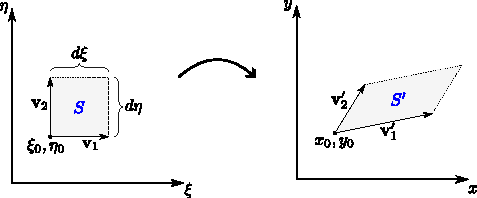
\includegraphics[width=0.6\linewidth]{dxideta.pdf}
\caption{Преобразование элементарного объёма}
\label{fig:dxideta}
\end{figure}

Определитель матрицы Якоби (якобиан), взятый в конкретной точке параметрической плоскости $\vec\xi_0$, показывает,
во сколько раз увеличился элементарный объём около этой точки в результате преобразования.
Действительно, рассмотрим два перпендикулярных элементарных вектора
в параметрической системе координат: $\vec v_1 = (d\xi, 0)$ и $\vec v_2 = (0, d\eta)$
отложенных от точки $\vec\xi_0$ (см.~\figref{fig:dxideta}).
В результате преобразования по формуле \cref{eq:jacobi_linear} 
получим следующие преобразования концевых точек и векторов:
\begin{align*}
& (\xi_0, \eta_0) \to (x_0, y_0), \\
& (\xi_0 + d\xi, \eta_0) \to (x_0 + J_{11} d\xi, y_0 + J_{21} d\xi) \hence \vec v_1 \to \vec v'_1 = (J_{11} d\xi, J_{21} d\xi), \\
& (\xi_0 , \eta_0 + d\eta) \to (x_0 + J_{12} d\eta, y_0 + J_{22} d\eta) \hence \vec v_2 \to \vec v'_2 = (J_{12} d\eta, J_{22} d\eta).
\end{align*}
Элементарный объём равен площади параллелограмма, построенного
на элементарных векторах.
В параметрической плоскости согласно \cref{eq:vec_cross_2d} получим 
$$ |S| = \vec v_1 \times \vec v_2 = d\xi d\eta,$$
и аналогично для физической плоскости:
$$
|S'| = \vec v'_1 \times \vec v'_2 = (J_{11} J_{22} - J_{12} J_{21})d\xi d\eta = |J| d\xi d\eta
$$
Сравнивая два последних соотношения приходим к выводу,
что элементарный объём в результате преобразования увеличился в $|J|$ раз. Тогда можно записать
\begin{equation}
\label{eq:dxdy_dxideta}
dx\,dy = |J|\,d\xi\,d\eta
\end{equation}

\subsubsubsection{Дифференцирование в параметрической плоскости}
Пусть задана некоторая функция $f(x, y)$. Распишем её производную по
параметрическим координатам:
\begin{align*}
&\dfr{f}{\xi} = \dfr{f}{x}\dfr{x}{\xi} + \dfr{f}{y}\dfr{y}{\xi}, \\
&\dfr{f}{\eta} = \dfr{f}{x}\dfr{x}{\eta} + \dfr{f}{y}\dfr{y}{\eta}.
\end{align*}
Вспоминая определение \cref{eq:jacobi_matrix_2d}, запишем
\begin{equation*}
\left(\begin{array}{c}
  \ddfr{f}{\xi} \\[10pt]
  \ddfr{f}{\eta}
  \end{array}
\right) = 
J^T 
\left(
  \begin{array}{c}
  \ddfr{f}{x} \\[10pt]
  \ddfr{f}{y}
  \end{array}
\right) =
\left(
  \begin{array}{cc}
    J_{11} & J_{21} \\[10pt]
    J_{12} & J_{22}
  \end{array}
\right)
\left(
  \begin{array}{c}
  \ddfr{f}{\xi} \\[10pt]
  \ddfr{f}{\eta}
  \end{array}
\right)
\end{equation*}
Обратная зависимость примет вид
\begin{equation*}
\left(\begin{array}{c}
  \ddfr{f}{x} \\[10pt]
  \ddfr{f}{y}
  \end{array}
\right) = 
\left(J^T\right)^{-1}
\left(
  \begin{array}{c}
  \ddfr{f}{\xi} \\[10pt]
  \ddfr{f}{\eta}
  \end{array}
\right) =
\frac{1}{|J|}
\left(
  \begin{array}{cc}
    J_{22} & -J_{21} \\[10pt]
    -J_{12} & J_{11}
  \end{array}
\right)
\left(
  \begin{array}{c}
  \ddfr{f}{\xi} \\[10pt]
  \ddfr{f}{\eta}
  \end{array}
\right)
\end{equation*}

\subsubsubsection{Интегрирование в параметрической плоскости}
Пусть в физической области $x, y$ задана область $D_x$.
Интеграл функции $f(x, y)$ по этой области
можно расписать, используя замену \cref{eq:dxdy_dxideta}
\begin{equation}
\label{eq:dxideta_integral}
\int\limits_{D_{x}}f(x, y)\,dxdy = \int\limits_{D_{\xi}}f(\xi, \eta) \, |J(\xi, \eta)|d\xi d\eta,
\end{equation}
где $f(\xi, \eta) = f(x(\xi, \eta), y(\xi, \eta))$, а $D_\xi$ -- образ области $D_x$ в параметрической плоскости.

\subsubsubsection{Двумерное линейное преобразование. Параметрический треугольник}
\label{sec:lintri_transform}
\begin{figure}[h!]
\centering
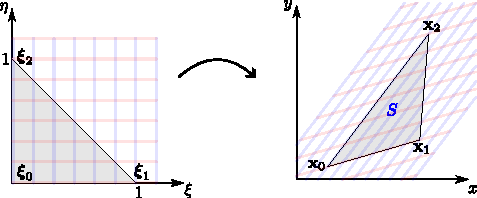
\includegraphics[width=0.6\linewidth]{lintri_transform.pdf}
\caption{Преобразование из параметрического треугольника}
\label{fig:lintri_transform}
\end{figure}
Рассмотрим двумерное преобразование, при котором
определяющие функции являются линейными. То есть представимыми в виде
\begin{align*}
x(\xi, \eta) = A_x \xi + B_x \eta + C_x, \\
y(\xi, \eta) = A_y \xi + B_y \eta + C_y.
\end{align*}
Для определения шести констант, определяющих это преобразование,
достаточно выбрать три любые (не лежащие на одной прямой) точки:
$(\xi_i, \eta_i) \to (x_i, y_i)$ для $i=0,1,2$.
В результате получим систему из шести линейных уравнений (три точки по две координаты),
из которой находятся конcтанты $A_{x,y}, B_{x,y}, C_{x,y}$.
Пусть три точки в параметрической плоскости
образуют единичный прямоугольный треугольник (\figref{fig:lintri_transform}):
\begin{equation*}
\xi_0, \eta_0 = (0, 0),\quad
\xi_1, \eta_1 = (1, 0),\quad
\xi_2, \eta_2 = (0, 1).
\end{equation*}
Тогда система линейных уравнений примет вид
\begin{align*}
&x_0 = C_x,       \quad y_0 = C_y, \\
&x_1 = A_x + C_x, \quad y_1 = A_y + C_y, \\
&y_2 = B_x + C_x, \quad y_2 = B_y + C_y.
\end{align*}
Определив коэффициенты преобразования их этой системы, окончательно запишем преобразование
\begin{equation}
\label{eq:lintri_transform}
\begin{aligned}
&x(\xi, \eta) = (x_1 - x_0)\xi + (x_2 - x_0) \eta + x_0,\\
&y(\xi, \eta) = (y_1 - y_0)\xi + (y_2 - y_0) \eta + y_0.\\
\end{aligned}
\end{equation}
Матрица Якоби этого преобразования \cref{eq:jacobi_matrix_2d}
не будет зависеть от параметрических координат $\xi, \eta$:
\begin{equation}
\label{eq:lintri_jacobi_matrix}
J = \left(
\begin{array}{cc}
x_1 - x_0 & x_2 - x_0 \\
y_1 - y_0 & y_2 - y_0 \\
\end{array}
\right).
\end{equation}
Якобиан преобразования будет равен удвоенной площади треугольника $S$, составленного из определяющих точек в физической плоскости:
\begin{equation}
\label{eq:lintri_jacobian}
|J| = (x_1 - x_0) (y_2 - y_0) - (y_1 - y_0) (x_2 - x_0) = (\vec x_1 - \vec x_0) \times (\vec x_2 - \vec x_0) = 2 |S|.
\end{equation}
Распишем интеграл по треугольнику $S$ по формуле \cref{eq:dxideta_integral}.
Вследствии линейности преобразования якобиан постоянен и, поэтому, его можно вынести его из-под интеграла:
\begin{equation}
\label{eq:lintri_integral}
\int\limits_{S}f(x, y)\,dxdy = |J|\int\limits_0^1 \int\limits_0^{1-\xi} f(\xi, \eta) d\eta d\xi.
\end{equation}

\subsubsubsection{Двумерное билинейное преобразование. Параметрический квадрат}
\label{sec:bilinquad_transform}
\begin{figure}[h!]
\centering
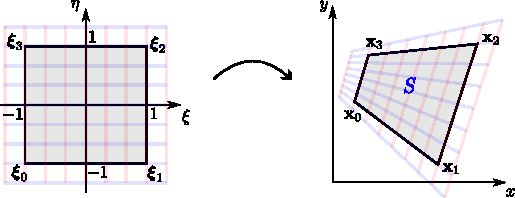
\includegraphics[width=0.6\linewidth]{bilinquad_transform.pdf}
\caption{Преобразование из параметрического квадрата}
\label{fig:bilinquad_transform}
\end{figure}

\subsubsubsection{Трёхмерное линейное преобразование. Параметрический тетраэдр}
TODO

\subsubsection{Свойства многоугольника}
\subsubsubsection{Площадь многоугольника}
\label{sec:polygon_area} 

\begin{figure}[h!]
\centering
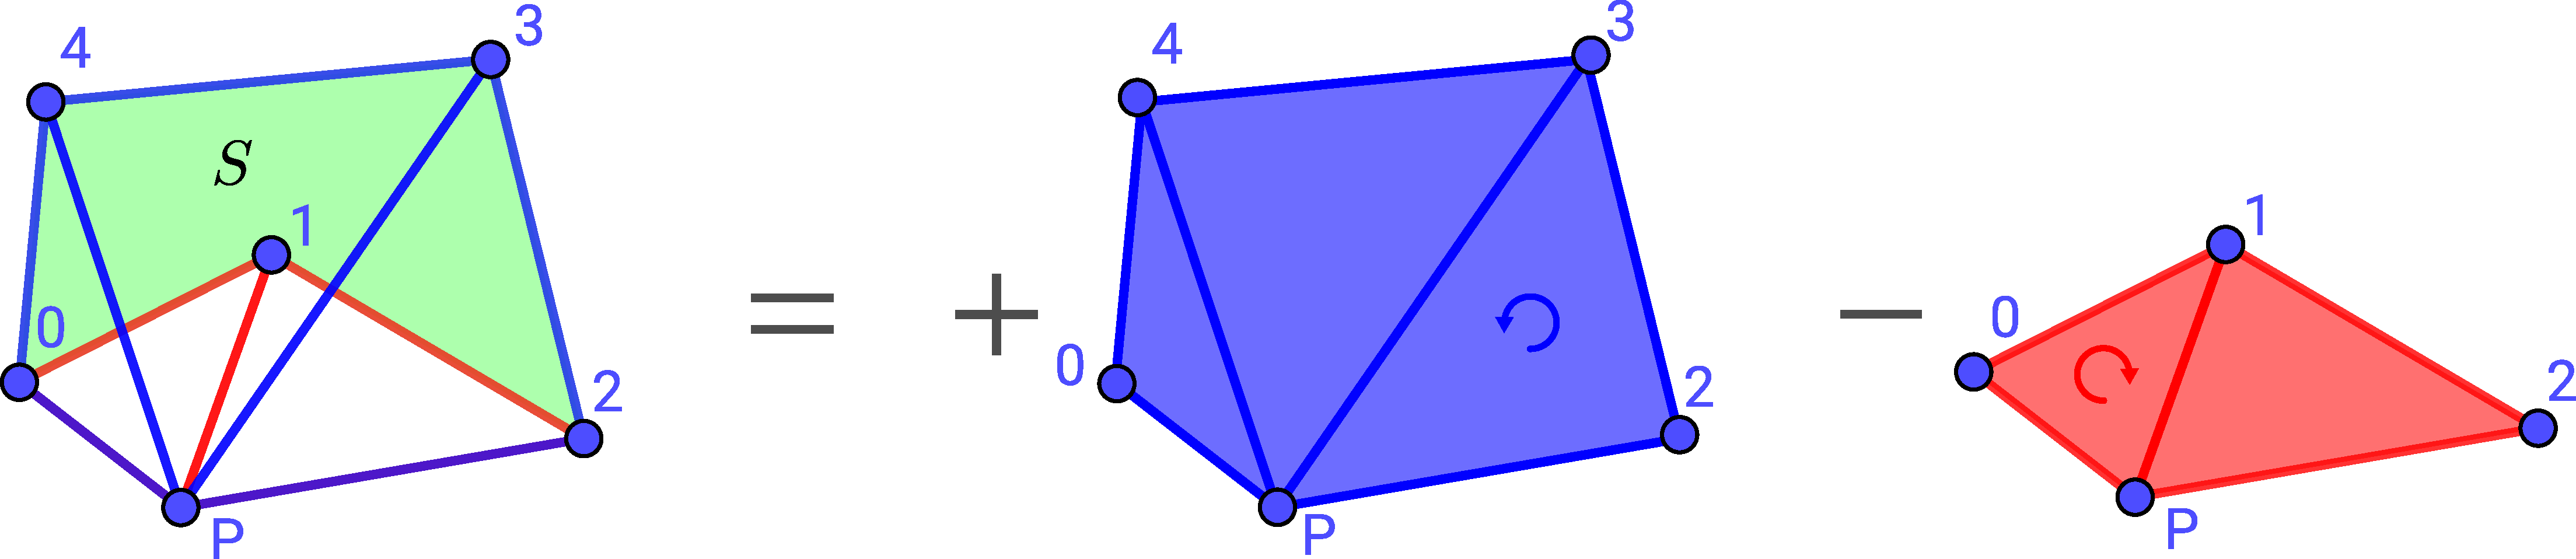
\includegraphics[width=0.7\linewidth]{polygon_area.pdf}
\caption{Площадь произвольного многоугольника}
\label{fig:polygon_area}
\end{figure}

Рассмотрим произвольный несамопересекающийся $N$-угольник $S$,
заданный координатами своих узлов $\vec x_i$, $i=\overline{0, N-1}$,
пронумерованных последовательно против часовой стрелки (\figref{fig:polygon_area}).
Далее введём произвольную точку $\vec p$ и 
от этой точки будем строить ориентированные треугольники до граней многоугольника:
$$
\triangle^p_i = (\vec p, \vec x_i, \vec x_{i+1}), \quad i=\overline{0, N-1},
$$
(для корректности записи будем считать, что $\vec x_N = \vec x_0$).
Тогда площадь исходного многоугольника $S$ будет равна сумме
знаковых площадей треугольников $\triangle^p_i$:
$$
|S| = \sum_{i=0}^{N-1} |\triangle^p_i|, \qquad |\triangle^p_i| = \frac{(\vec x_i - \vec p) \times (\vec x_{i+1} - \vec p)}{2}.
$$
Знак площади ориентированного треугольника зависит от направления закрутки его узлов:
она положительна для закрутки против часовой стрелки и отрицательна, если узлы пронумерованы по часовой стрелке.
В частности, на рисунке~\ref{fig:polygon_area} видно, что треугольники, отмеченные красным: $P01, P12$, будут
иметь отрицательную площадь, а синие треугольники $P23$, $P34$, $P40$ -- положительную. Сумма этих площадей
с учётом знака даст искомую площадь многоугольника.

Для сокращения вычислений воспользуемся произвольностью положения $\vec p$ и совместим
её с точкой $\vec x_0$. Тогда треугольники $\triangle^p_0$, $\triangle^p_{N-1}$
выродятся (будут иметь нулевую площадь).
Обозначим такую последовательную триангуляцию как
\begin{equation}
\label{eq:seq_polygon_triangulation}
\triangle_i = (\vec x_0, \vec x_i, \vec x_{i+1}), \qquad i=\overline{1,N-2}.
\end{equation}
Знаковая площадь ориентированного треугольника будет равна
\begin{equation}
\label{eq:seq_triangle_area}
|\triangle_i| = \frac{(\vec x_i - \vec x_0) \times (\vec x_{i+1} - \vec x_0)}{2}.
\end{equation}
Тогда окончательно формула определения площади примет вид
\begin{equation}
\label{eq:polygon_area}
|S| = \sum_{i=1}^{N-2}|\triangle_i|.
\end{equation}

\paragraph{Плоский полигон в пространтве} Если плоский полигон $S$ расположен в трёхмерном пространстве,
то правая часть формулы \cref{eq:seq_triangle_area} согласно определению векторного произведения в трёхмерном пространстве \cref{eq:vec_cross}
-- есть вектор.
Чтобы получить скалярную площадь, нужно спроецировать этот вектор на единичную нормаль к плоскости
многоугольника:
$$
\vec n = \frac{\vec k}{|\vec k|}, \qquad \vec k = (\vec x_1 - \vec x_0) \times (\vec x_2 - \vec x_0).
$$
Эта формула записана из предположения, что узел $\vec x_2$ не лежит
на одной прямой с узлами $\vec x_0$, $\vec x_1$. Иначе вместо $\vec x_2$ нужно
выбрать любой другой узел, удовлетворяющий этому условию.
Тогда площадь ориентированного треугольника, построенного
в трёхмерном пространстве запишется через смешанное произведение:
\begin{equation}
\label{eq:seq_triangle_area_3d}
|\triangle_i| = \frac{\left((\vec x_i - \vec x_0) \times (\vec x_{i+1} - \vec x_0) \right)\cdot \vec n}{2}.
\end{equation}
Формула для определения площади полигона \cref{eq:polygon_area} будет по прежнему верна.
При этом итоговый знак величины $S$ будет положительным,
если закрутка полигона положительная (против часовой стрелки) при взгляде со стороны
вычисленной нормали $\vec n$.

\subsubsubsection{Интеграл по многоугольнику}
\label{sec:polygon_integral} 
Рассмотрим интеграл функции $f(x,y)$ по $N$-угольнику $S$, заданному последовательными координатами своих узлов $\vec x_i$.
Введём последовательную триангуляцию согласно \cref{eq:seq_polygon_triangulation}.
Тогда интеграл по многоугольнику можно расписать как сумму интегралов по ориентированным треугольникам:
\begin{equation}
\label{eq:seq_triangulation_integral}
\arint{f(x,y)}{S}{xdy} = \sum_{i=1}^{N-2} \arint{f(x,y)}{\triangle_i}{xdy}.
\end{equation}
Далее для вычисления интегралов в правой части
воспользуемся преобразованием к параметрическому треугольнику (п.~\ref{sec:lintri_transform}).
Следуя формуле интегрирования \cref{eq:lintri_integral}, распишем
интеграл по $i$-ому треугольнику:
\begin{equation*}
\arint{f(x,y)}{\triangle_i}{xdy} = |J_i| \int\limits_{0}^{1}\int\limits_{0}^{1-\xi} f_i(\xi, \eta) \, d\eta d\xi,
\end{equation*}
где якобиан $|J_i|$ согласно \cref{eq:lintri_jacobian} есть удвоенная площадь ориентированного треугольника $\triangle_i$
(положительная при закрутке против часовой стрелке и отрицаетельная иначе):
\begin{equation*}
|J_i| = 2|\triangle_i| = (\vec x_i - \vec x_0) \times (\vec x_{i+1} - \vec x_0),
\end{equation*}
а функция $f_i(\xi, \eta)$ есть функция от преобразованных согласно \cref{eq:lintri_transform}
переменных:
\begin{equation*}
f_i(\xi, \eta) = f\left(\left(\vec x_i - \vec x_0\right)\xi + \left(\vec x_{i+1} - \vec x_0\right)\eta + \vec x_0\right).
\end{equation*}
Окончательно запишем
\begin{equation}
\label{eq:polygon_integral}
\arint{f(x,y)}{S}{xdy} = 2 \sum_{i=1}^{N-2}
    |\triangle_i| \int\limits_{0}^{1}\int\limits_{0}^{1-\xi} f_i(\xi, \eta) \, d\eta d\xi.
\end{equation}
Отметим, что эта формула работает и в том случае, когда
полигон расположен в трёхмерном пространстве
(знаковую площадь при этом следует вычислять по \cref{eq:seq_triangle_area_3d}).

\subsubsubsection{Центр масс многоугольника}
\label{sec:polygon_center} 
По определению, координаты центра масс $\vec c$ области $S$ равны среднеинтегральным значениям координатных функций. То есть
\begin{equation*}
c_x = \frac{1}{|S|}\int\limits_{S} x \, dxdy,
\quad 
c_y = \frac{1}{|S|}\int\limits_{S} y \, dxdy.
\end{equation*}
Далее распишем интеграл в правой части через последовательную триангуляцию согласно
\cref{eq:seq_triangulation_integral} с учётом линейного преобразования
\cref{eq:lintri_transform}:
\begin{align*}
\int\limits_{S} x \, dxdy &= \sum_{i=1}^{N-2} \int\limits_{\triangle_i} x \, dxdy\\
                          &= \sum_{i=1}^{N-2} |J_i| \int\limits_0^1\int\limits_0^{1-\xi} ((x_i - x_0)\xi + (x_{i+1} - x_0)\eta + x_0)\, d\eta d\xi\\
                          &= \sum_{i=1}^{N-2} \frac{|J_i|}{2}\frac{x_0 + x_i + x_{i+1}}{3}\\
                          &= \sum_{i=1}^{N-2} |\triangle_i|\frac{x_0 + x_i + x_{i+1}}{3}.
\end{align*}
Итого, с учётом \cref{eq:polygon_area}, координаты центра масс примут вид
\begin{align*}
&\vec c = \dfrac{\displaystyle\sum_{i=1}^{N-2} \dfrac{\vec x_0 + \vec x_i + \vec x_{i+1}}{3}|\triangle_i|}{\displaystyle\sum_{i=1}^{N-2} |\triangle_i|}.
\end{align*}
Если полигон расположен в двумерном пространстве $xy$, то знаковая площадь треугольников
вычисляется по формуле \cref{eq:seq_triangle_area}.
В случае трёхмерного пространтва должна использоваться формула \cref{eq:seq_triangle_area_3d}.

\subsubsection{Свойства многогранника}
\subsubsubsection{Объём многогранника}
\label{sec:polyhedron_volume} 
TODO
\subsubsubsection{Интеграл по многограннику}
\label{sec:polyhedron_integral} 
TODO
\subsubsubsection{Центр масс многогранника}
\label{sec:polyhedron_center} 
TODO

\subsubsection{Поиск многоугольника, содержащего заданную точку}
TODO


\section{Работа с инфраструктурой проекта CFDCourse}

\subsection{Сборка и запуск}
\subsubsection{Сборка проекта CFDCourse}

Описанная ниже процедура собирает проект в отладочной конфигурации.
Для проведения необходимых модификаций для сборки релизной версии смотри \ref{sec:release-build}.

\subsubsubsection{Подготовка}
\label{sec:install-prep}
\begin{enumerate}
\item
Для сборки проекта необходимо установить \ename{git} и \ename{cmake>=3.0}

В Windows необходимо скачать и установить диструбутивы:
\begin{itemize}
\item
\url{https://github.com/git-for-windows/git/releases/download/v2.43.0.windows.1/Git-2.43.0-64-bit.exe}
\item
\url{https://github.com/Kitware/CMake/releases/download/v3.28.3/cmake-3.28.3-windows-x86\_64.msi}
\end{itemize}

При установке cmake проследите, что бы путь к \ename{cmake.exe} сохранился в системных путях.
Msi установщик спросит об этом в диалоге.

В {\bf линуксе} используйте менеджеры пакетов, предоставляемые вашим дистрибутивом.
Также проследите чтобы были доступны компиллятор \ename{g++} и отладчик \ename{gdb}.

\item
Создайте папку в системе для репозиториев. Например \ename{D:/git_repos/}

\item
Возьмите необходимые заголовочные библиотеки boost из \url{https://disk.yandex.ru/d/GwTZUvfAqPsZBQ}
и распакуйте архив в папку для репозиториев (D:/git\_repos/boost).
Проследите, чтобы внутри папки boost сразу шли папки с кодом (\ename{accumulators}, \ename{algorithm}, ...)
и заголовочные файлы (\ename{align.hpp}, \ename{aligned_storage.hpp}, ...)
без дополнительных уровней вложения.

\item
Откройте терминал (git bash в Windows).

\item
С помощью команды cd в терминале перейдите в папку для репозиториев
\begin{shelloutput}
> cd D:/git_repos
\end{shelloutput}

\item
Клонируйте репозиторий
\begin{shelloutput}
> git clone https://github.com/kalininei/CFDCourse25
\end{shelloutput}
В директории (\ename{D:/git_repos} в примере) появится папка \ename{CFDCourse25}, которая является корневой папкой проекта
\end{enumerate}

\subsubsubsection{VisualStudio}
\label{sec:vs-build}

\begin{enumerate}
\item
Cоздайте папку build в корне проекта СFDCourse25

\item
Скопируйте скрипт winbuild64.bat в папку build. Далее вносить изменения
только в скопированном файле.

\item
Скрипт написан для версии \ename{Visual Studio 2019}. Если используется другая версия,
измените в скрипте значение переменной \cvar{CMGenerator} на соответствующие вашей версии.
Значения для разных версий Visual Studio написаны ниже
\begin{shelloutput}
SET CMGenerator="Visual Studio 17 2022"
SET CMGenerator="Visual Studio 16 2019"
SET CMGenerator="Visual Studio 15 2017"
SET CMGenerator="Visual Studio 14 2015"
\end{shelloutput}

\item
Запустите скрипт \ename{winbuild64.bat} из папки \ename{build}. Нужен доступ к интернету.
В процессе будет скачано около 200Мб пакетов, поэтому первый запуск может занять время

\item
После сборки в папке \ename{build} появится проект \ename{VisualStudio} \ename{cfdcourse25.sln}.
Его нужно открыть в \ename{VisualStudio}.
Дерево решения должно иметь следующий вид:
\begin{center}
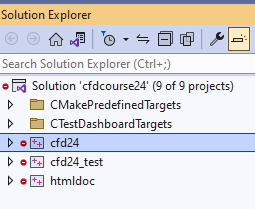
\includegraphics[width=0.3\linewidth]{vs_solution_explorer.png}
\end{center}
Проекты:
\begin{itemize}
\item \ename{cfd25} -- расчётная библиотека
\item \ename{cfd25_test} -- модульные тесты для расчётных функций
\end{itemize}

\item
Проект \ename{cfd25_test} необходимо назначить запускаемым проектом. Для этого нажать правой кнопкой мыши по проекту и в выпадающем меню
выбрать соответствующий пункт. После этого заголовок проекта должен стать жирным.
\begin{center}
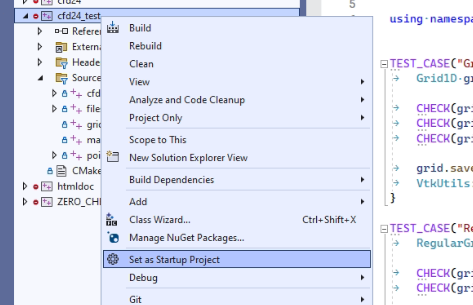
\includegraphics[width=0.5\linewidth]{win_startup_project.png}
\end{center}

\item
Скомпиллировать решение. Несколько способов:
\begin{itemize}
\item \ename{Ctrl+Shift+B},
\item \ename{Build->Build Solution} в основном меню,
\item \ename{Build Solution} в меню решения в дереве решения,
\item \ename{Build} в меню проекта \ename{cfd25_test}.
\end{itemize}

\item
Запустить тесты (проект \ename{cfd25_test}) нажав \ename{F5} (или кнопку отладки в меню).
После отработки должно высветиться сообщение об успешном прохождении всех тестов.

\item
Бинарные файлы будут скомпиллированы в папку \ename{CFDCourse25/build/bin/Debug}.
В случае работы через отладчик выходная директория, куда будут скидываться все файлы (в частности, vtk),
должна быть \ename{CFDCourse25/build/src/test/}.
\end{enumerate}

\subsubsubsection{VSCode}
\label{sec:vscode-build}

\begin{enumerate}
\item
Открыть корневую папку проека через \ename{File->Open Folder}
\item
Установить предлагаемые расширения cmake, c++
\item
Для настройки отладки создайте конфигурацию launch.json следующего вида
\begin{center}
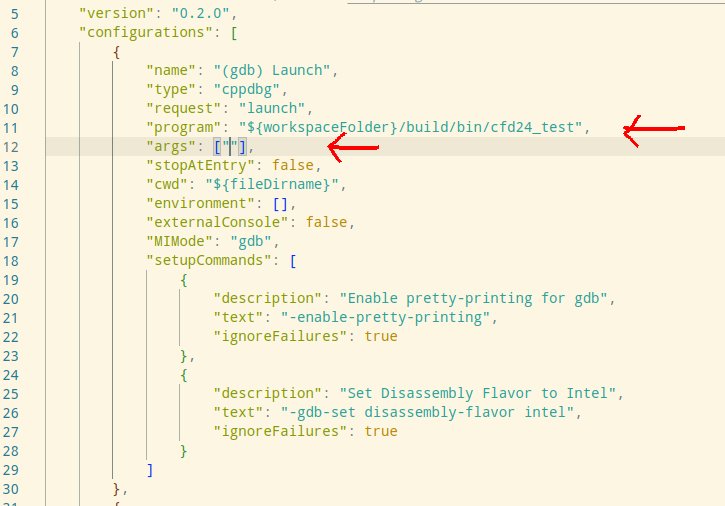
\includegraphics[width=0.7\linewidth]{vscode_launch_json.png}
\end{center}
\begin{itemize}
\item
Для этого перейдите в меню \ename{Run and Dubug} (\ename{Ctrl+Shift+D}), нажмите
\ename{create launch.json}, выберите пункт \ename{Node.js}.
\item
После этого в корневой папке появится файл \ename{.vscode/launch.json}.
\item
Откройте этот файл в \ename{vscode}, нажмите \ename{Add configuration}, \ename{(gdb) Launch} или \ename{(Windows) Launch} в зависимости от ОС.
\item
Далее напишите имя программы как показано на картинке.
\item
Используйте поле args для установки аргументов запуска.
\item
Выберите созданную конфигурацию для запуска отладчика по \ename{F5}
\begin{center}
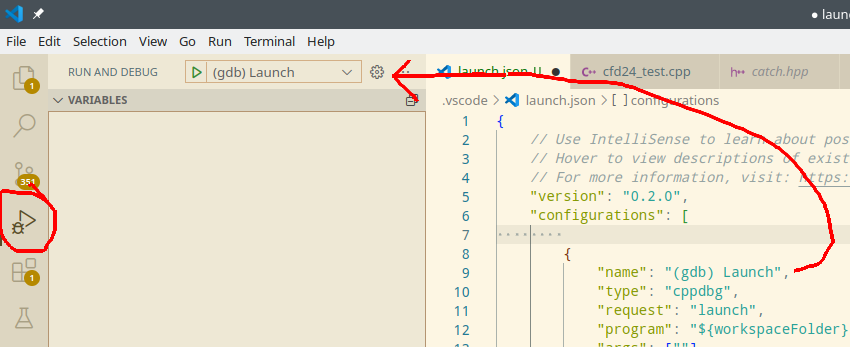
\includegraphics[width=0.7\linewidth]{vscode_launch.png}
\end{center}
\end{itemize}

На скриншотах представлены настройки в случае работы в линуксе. Для работы под виндоус 
\begin{shelloutput}
"name" : "(Windows) Launch",
"program": "${workspaceFolder}/build/bin/Debug/cfd25_test.exe"
\end{shelloutput}
\end{enumerate}

\subsubsection{Запуск конкретного теста}

По умолчанию программа \ename{cfd25_test} прогоняет все объявленные в проекте тесты. Иногда может возникнуть необходимость
запустить только конкретный тест в целях отладки или проверки.
Для этого нужно передать программе аргумент с тегом для этого теста.

Тег для теста -- это второй аргумент в макросе \cvar{TEST_CASE}, записанный в квадратных скобках.
Добавлять нужно вместе со скобками. Например, \cvar{[ping]}.

Чтобы добавить аргумент в \ename{VisualStudio}, необходимо в контекстном меню проекта \ename{cfd25_test} выбрать опции отладки
\begin{center}
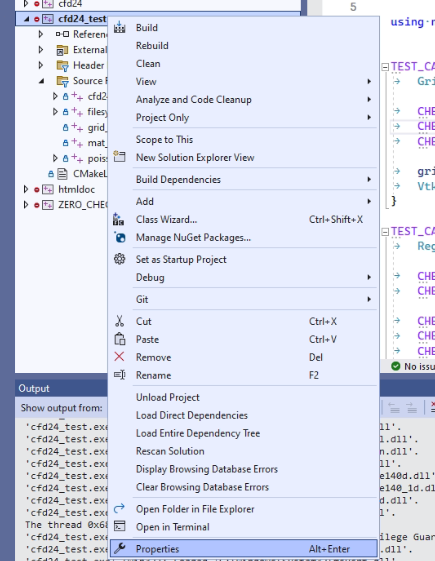
\includegraphics[width=0.7\linewidth]{win_debug_args_1.png}
\end{center}
и там в поле Аргументы прописать нужный тэг.
\begin{center}
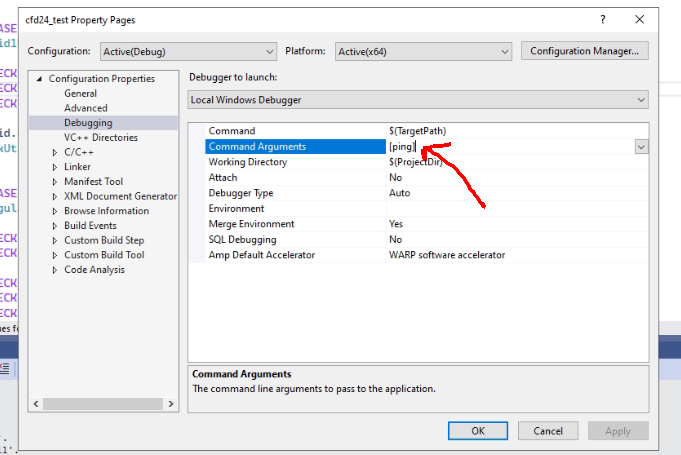
\includegraphics[width=0.9\linewidth]{win_debug_args_2.png}
\end{center}

В \ename{VSCode} аргументы нужно добавлять в файле \ename{.vscode/launch.json} в поле args в кавычках
(см. картинку \ref{sec:vscode-build} с настройками launch.json).

\subsubsection{Сборка релизной версии}
\label{sec:release-build}

Релизная сборка программ даёт многократное увеличение производительности,
но при этом отладка приложений в таком режиме невозможна.

{\bf Visual Studio}
\begin{enumerate}
\item Создать папку \ename{build-release} рядом с папкой \ename{build}.
\item Скопировать в неё файл \ename{winbuild64.bat} из папки \ename{build}. 
\item В скопированном файле произвести замену \cvar{Debug} на \cvar{Release}
\begin{shelloutput}
-DCMAKE_BUILD_TYPE=Release ..
\end{shelloutput}
\item Запустить \ename{winbuild64.bat} из новой папки
\item Открыть \ename{build-release/cfdcourse25.sln} в \ename{Visual Studio}
\item В проекте студии установить релизную сборку
\begin{center}
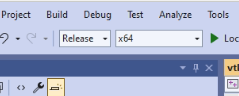
\includegraphics[width=0.5\linewidth]{release_build.png}
\end{center}
\item Это новое решение, не связанное настройками с \ename{debug}-версией.
      Поэтому нужно заново настроить запускускаемым проектом \ename{cfd_test}
      и, если нужно, настроить аргументы отладки.
\item Бинарные файлы будут скомпиллированы в папку \ename{CFDCourse25/build_release/bin/Release}.
      В случае работы через отладчик выходная директория -- \ename{CFDCourse25/build_release/src/test/}.
\end{enumerate}

{\bf VSCode}
\begin{enumerate}
\item Выбрать релизную сборку в \ename{build variant}
\item Нажать \ename{Build}
\item Нажать \ename{Launch}
\begin{center}
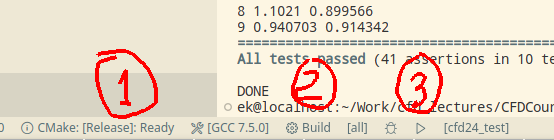
\includegraphics[width=0.5\linewidth]{release_build_2.png}
\end{center}
\end{enumerate}

\subsection{Git}
\subsubsection{Основные команды}
Все команды выполнять в терминале (\ename{git bash} для виндоус),
находясь в корневой папке проета CFDCourse24.
\begin{itemize}
\item
  Для {\bf смены директории} использовать команду \ename{cd}. Например, находясь в папке \ename{A} перейти в папку \ename{A/B/C}
  \begin{shelloutput}
> cd B/C
  \end{shelloutput}
\item
  {\bf Подняться} на директорию выше
  \begin{shelloutput}
> cd ..
  \end{shelloutput}
\item
  {\bf Просмотр статуса} текущего репозитория: текущую ветку, все изменённые файлы и т.п.
  \begin{shelloutput}
> git status
  \end{shelloutput}
\item
  {\bf Сохранить и скоммитить} изменения в текущую ветку
  \begin{shelloutput}
> git add .
> git commit -m "message"
  \end{shelloutput}

  ``message'' -- произвольная информация о текущем коммите, которая будет приписана к этому коммиту
\item
  {\bf Переключиться на ветку} main
  \begin{shelloutput}
> git checkout main
  \end{shelloutput}

  работает только в том случае, если все файлы скоммичены и статус ветки 'Up to date'
\item
  {\bf Создать новую ветку} ответвлённую от последнего коммита текущей ветки и переключиться на неё
  \begin{shelloutput}
> git checkout -b new-branch-name
  \end{shelloutput}

  new-branch-name -- имя новой ветки. Пробелы не допускаются

  Эта комманда работает даже если есть нескоммиченные изменения. 
  Если необходимо скоммитить изменеия в новую ветку, сразу за этой командой нужно вызвать
  \begin{shelloutput}
> git add .
> git commit -m "message"
  \end{shelloutput}
\item
  {\bf Сбросить} все нескоммиченные изменения. Вернуть файлы в состояние последнего коммита
  \begin{shelloutput}
> git reset --hard
  \end{shelloutput}

  Все изменения будут утеряны
\item
  {\bf Получить последние изменения} из удалённого хранилища с обновлением текущей ветки
  \begin{shelloutput}
> git pull
  \end{shelloutput}
  Работает только если статус текущей ветки 'Up to date'.\\
  Если требуется получить изменения, но не обновлять локальную ветку:
  \begin{shelloutput}
> git fetch
  \end{shelloutput}
  Обновленная ветка будет доступна по имени origin/{имя ветки}.
\item
  {\bf Просмотр истории} коммитов в текущей ветке (последний коммит будет наверху)
  \begin{shelloutput}
> git log
  \end{shelloutput}
\item
  {\bf Просмотр доступных веток} в текущем репозитории
  \begin{shelloutput}
> git branch
  \end{shelloutput}
\item
  {\bf Просмотр} актуального состояние дерева репозитория в gui режиме
  \begin{shelloutput}
> git gui
  \end{shelloutput}
  Далее в меню \ename{Repository->Visualize all branch history}.
  В этом же окне можно посмотреть изменения файлов по сравнению с последним коммитом.

  Альтернативно, при работе в виндоус можно установить программу GitExtensions и работать в ней.
\end{itemize}
  
\subsubsection{Порядок работы с репозиторием CFDCourse}

Основная ветка проекта -- \ename{main}. После каждой лекции (в течении 1-2 дней) в эту ветку будет отправлен коммит с сообщением \ename{after-lect{index}}.
Этот коммит будет содержать краткое содержание лекции,
задание по итогам лекции и необходимые для этого задания изменения кода.

Если предполагается работа с кодом на лекции, то перед лекцией в эту ветку будет отправлен коммит с сообщением \ename{before-lect{index}}.
Этот коммит содержит изменения кода для работы на лекции.

Таким образом, {\bf после лекции} необходимо выполнить следующие команды (находясь в ветке \ename{main})
\begin{shelloutput}
> git reset --hard  # очистить локальную копию от изменений,
                    # сделанных на лекции (если они не представляют ценности)
> git pull          # получить изменения
\end{shelloutput}

{\bf Перед началом лекции}, если была сделана какая то работа по заданиям,
\begin{shelloutput}
> git checkout -b work-lect{index}    # создать локальную ветку, содержащую задание
> git add .
> git commit -m "{свой комментарий}"  # скоммитить свои изменения в эту ветку
> git checkout main                   # вернуться на ветку main
> git pull                            # получить изменения
\end{shelloutput}

Даже если задание выполнено не до конца, вы в любой момент можете переключиться на ветку с заданием и его доделать
\begin{shelloutput}
> git checkout work-lect{index}
\end{shelloutput}

Если ничего не было сделано (или все изменения не представляют ценности), можно повторить алгоритм ``после лекции''.

\subsection{Paraview}

\subsubsection{Данные на одномерных сетках}
\label{sec:paraview-1d}

Заданные на сетке данные паравью показывает цветом.
Поэтому при загрузке одномерных сеток можно видеть картинку типа
\begin{center}
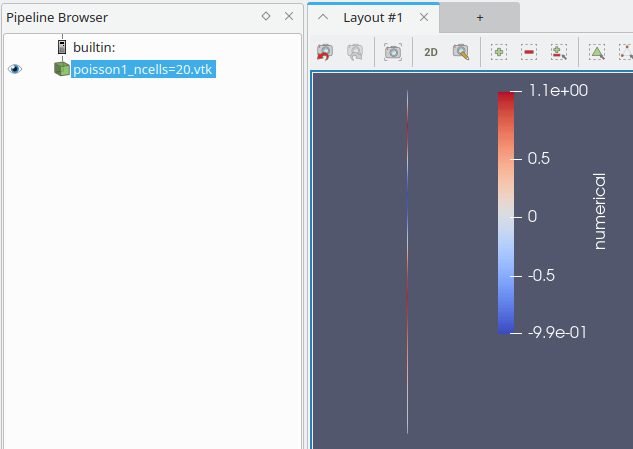
\includegraphics[width=0.5\linewidth]{howto_paraview_1d_1.png}
\end{center}
\paragraph{Развернуть изображение в плоскость xy}
\begin{center}
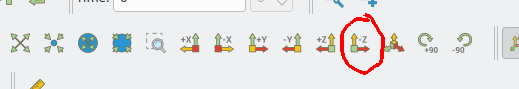
\includegraphics[width=0.5\linewidth]{howto_paraview_1d_2.png}
\end{center}
\paragraph{Отобразить данные в виде y-координаты} Для того, что бы данные отображались в качестве значения по оси ординат, к загруженному файлу необходимо
\begin{enumerate}
\item применить фильтр \ename{WarpByScalar} (В меню \ename{Filters->Alphabetical->Warp By Scalar})
\item в меню настройки фильтра указать поле данных, для отображения (numerical в примере ниже)
\item И настроить нормаль, вдоль которой будут проецироваться данные (в нашем случае ось y)
\end{enumerate}
\begin{center}
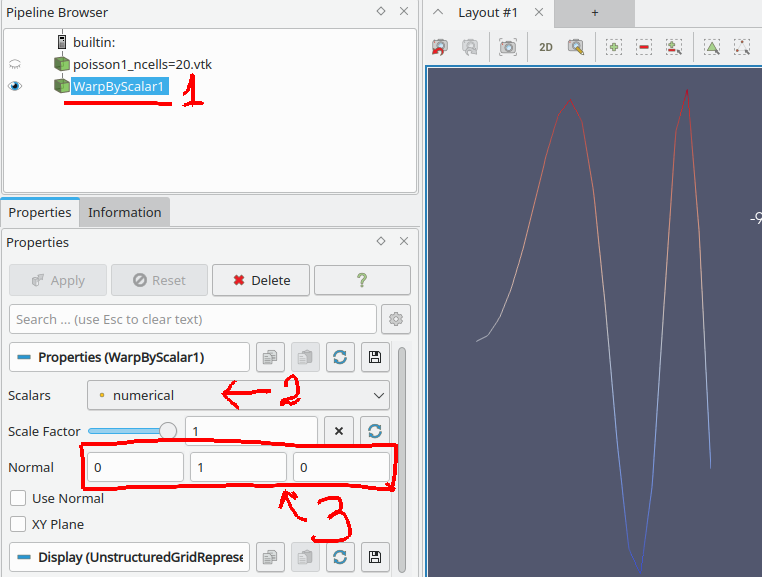
\includegraphics[width=0.5\linewidth]{howto_paraview_1d_3.png}
\end{center}

\paragraph{Цвет и толщина линии}
\begin{enumerate}
\item Включить подробные опции фильтра
\item Сменить стиль на \ename{Solid Color}
\item В меню \ename{Edit} выбрать желаемый цвет
\item В строке \ename{Line Width} указать толщину линии
\end{enumerate}
\begin{center}
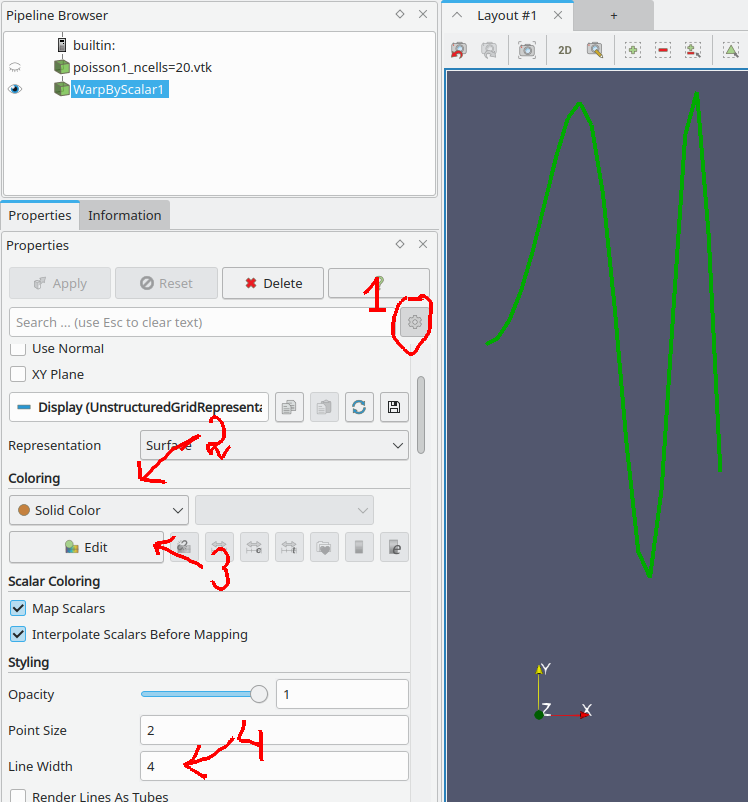
\includegraphics[width=0.6\linewidth]{howto_paraview_1d_4.png}
\end{center}

\paragraph{Настрока масштабов и отображение осей координат}
\begin{enumerate}
\item Отметье подробные настройки фильтра
\item В поле \ename{Transforming/Scale} Установите желаемые масштабы (в нашем случае растянуть в два раза по оси x)
\item Установите галку на отображение осей
\item откройте меню натройки осей
\item В нём включите подробные настроки
\item И также поставьте растяжение осей
\end{enumerate}
В случае, если масштабировать график не нужно, достаточно выполнить шаг 3.
\begin{center}
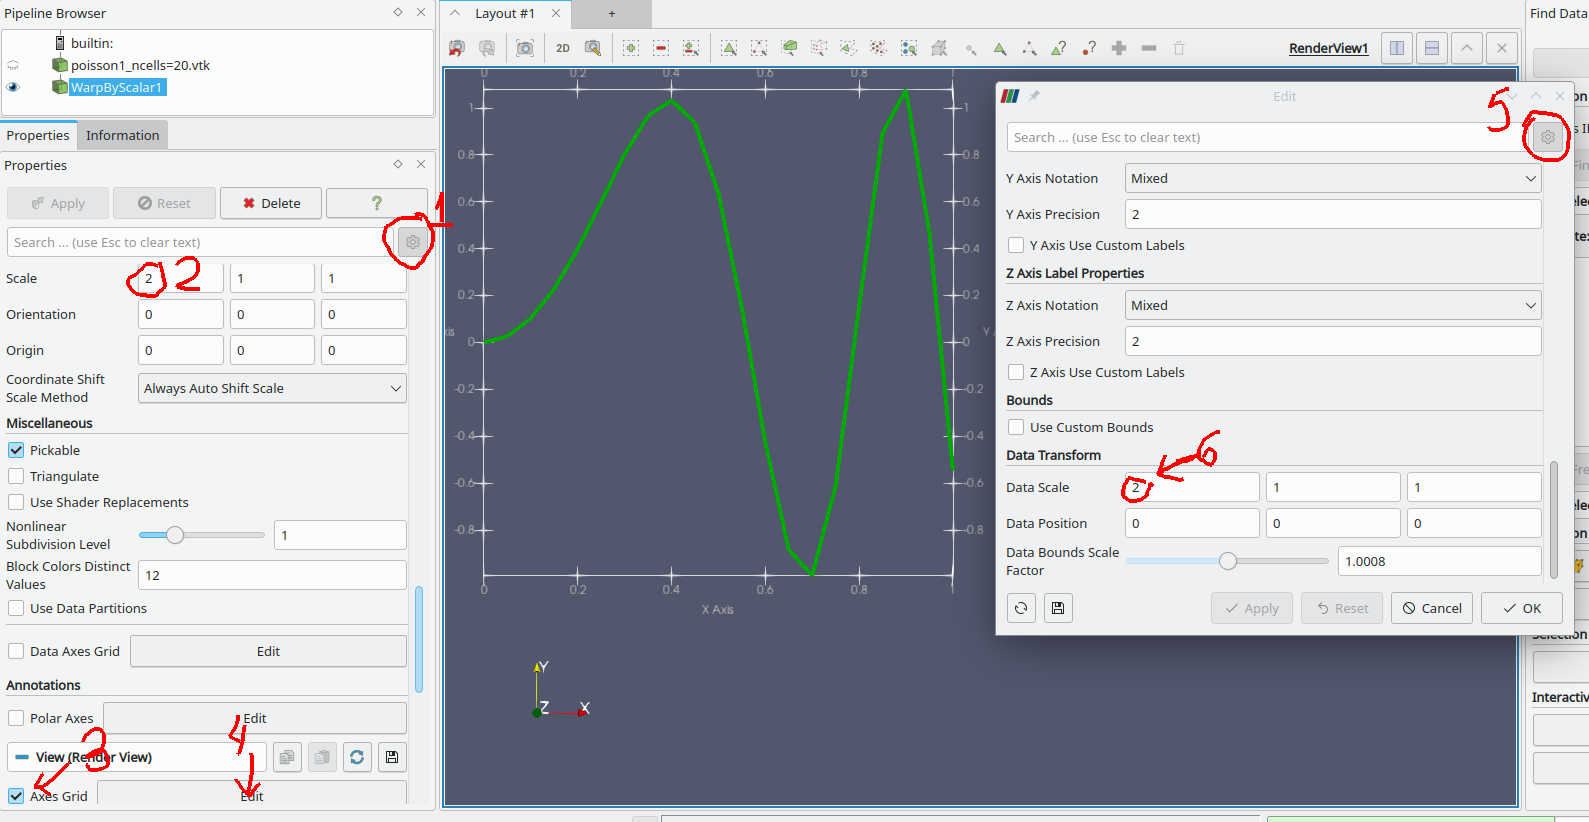
\includegraphics[width=0.9\linewidth]{howto_paraview_1d_5.png}
\end{center}

\paragraph{Построение графиков для нескольких данных}
Если требуется нарисовать рядом несколько графиков для разных данных из одного файла,
примените фильтр \ename{Warp By Scalar} для этого файла ещё раз, изменив поле \ename{Scalars} в настройке фильтра.
Для наглядности измените имя узла в Pipeline Browser на осмысленные
\begin{center}
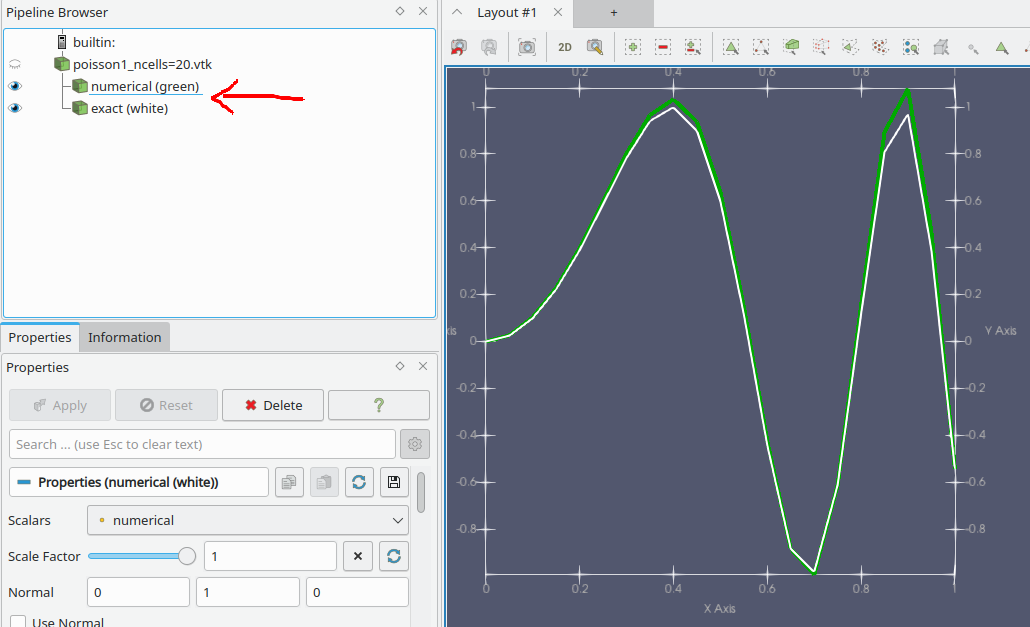
\includegraphics[width=0.8\linewidth]{howto_paraview_1d_6.png}
\end{center}

\paragraph{Обновление данных при изменении исходного файла}
В случае, если исходный файл был изменён, нужно в контекстном меню узла соответствующего файла
выбрать \ename{Reload Files} (или нажать F5). Если те же самые фильтры нужно применить для просмотра другого файла
нужно в этом меню нажать \ename{Change File}.
\begin{center}
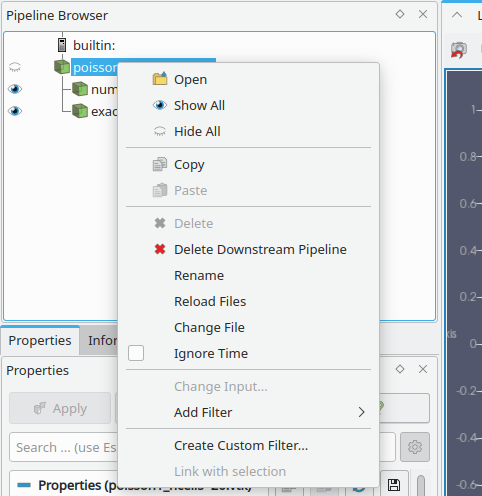
\includegraphics[width=0.4\linewidth]{howto_paraview_1d_7.png}
\end{center}

\subsubsection{Изолинии для двумерного поля}
\label{sec:paraview-isolines}

\begin{enumerate}
\item Нажмите иконку \ename{Contour} (или \ename{Filters/Contour})
      В настройках фильтра Contour by выберитее данные, по которым нужно строить изолинии.
\item В настройках фильтра удалите все существующие записи о значениях для изолиний
\item Добавьте равномерные значения. В появившемся меню установите необходимое количество изолиний и их диапазон.
\item Если необходимо, включите одновременное отображения цветного поля и изолиний.
\end{enumerate}

\begin{center}
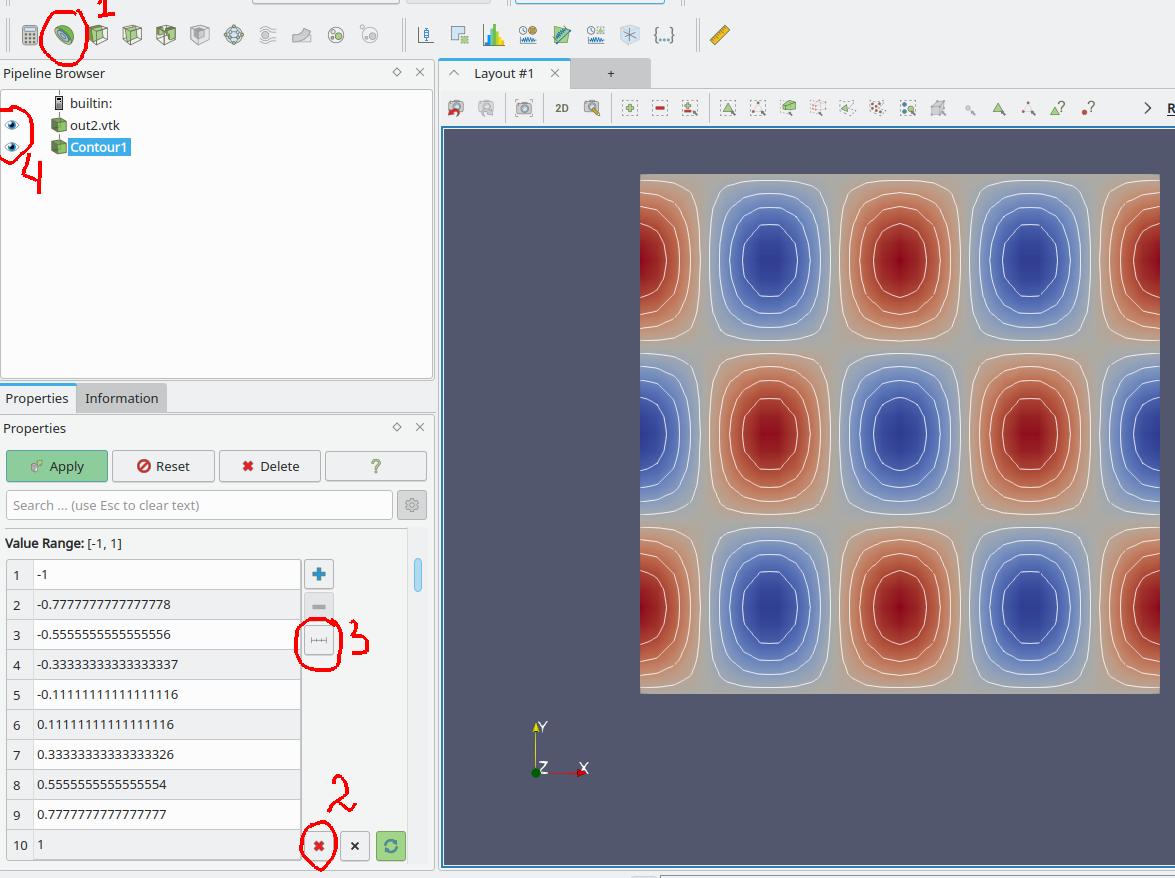
\includegraphics[width=0.7\linewidth]{howto_paraview_isolines_1.png}
\end{center}

\paragraph{Задание цвета и толщины изолинии}
В случае, если нужно сделать изолинии одного цвета, установите поле \ename{Coloring/Solid color} в 
настройках фильтра. Там же в меню \ename{Edit} можно выбрать цвет.
Для установления толщины линии включите подробные настройки и найдите там опцию \ename{Styling/Line Width}.
\begin{center}
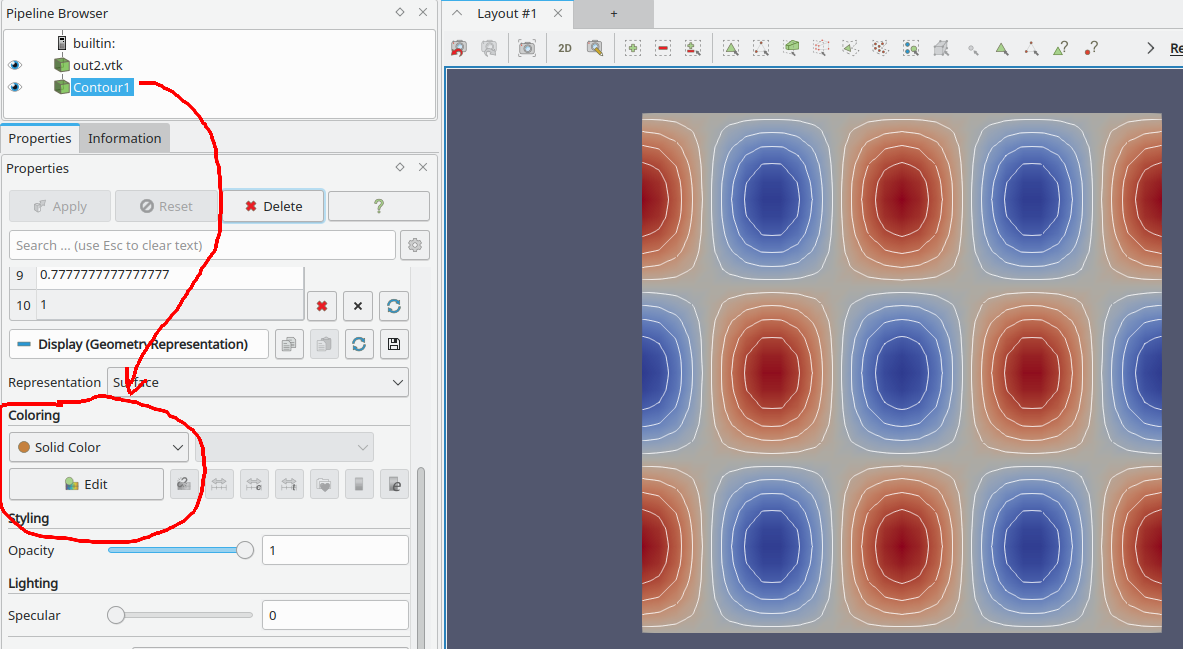
\includegraphics[width=0.7\linewidth]{howto_paraview_isolines_2.png}
\end{center}

\subsubsection{Данные на двумерных сетках в виде поверхности}
\label{sec:paraview-2d}

По аналогии с  одномерным графиком (п.~\ref{sec:paraview-1d}), двумерные поля так же
можно отобразить, проектируя данные на геометрическую координату для получения
объёмного графика. Для этого
\begin{enumerate}
\item Включите фильтр \ename{Filters/Warp By Scalar}
\item В настройках фильтра установите данные, которые будут проектироваться на координату z
\item Установите нормаль для проецирования (ось z)
\item Если нужно, выберите масштабирования для этой координаты
\item После нажатия \ename{Apply} включите трёхмерное отображение
\item Если данные не видно, обновите экран.
\end{enumerate}
\begin{center}
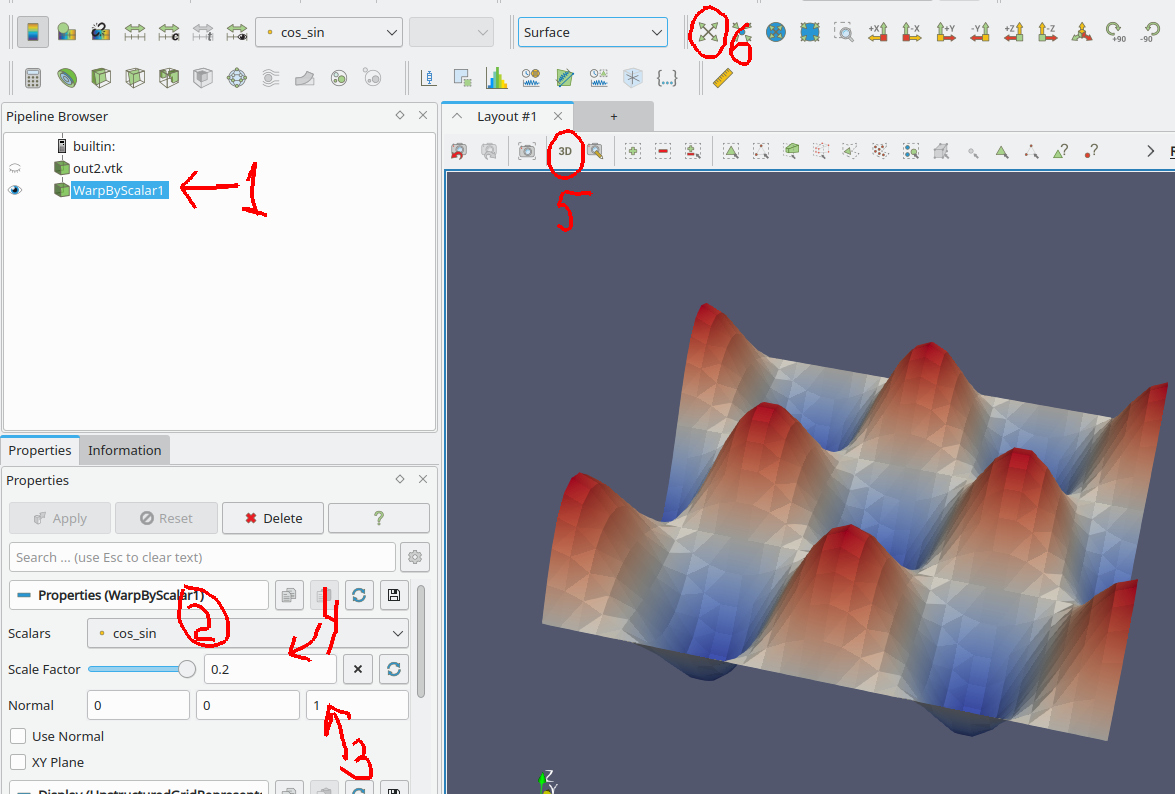
\includegraphics[width=0.9\linewidth]{howto_paraview_2d_as_3d.png}
\end{center}

\subsubsection{Числовых значения в точках и ячейках}
\label{sec:paraview-show-data}

Иногда в процессе отладки или анализа результатов расчёта
требуется знать точное значение поля в заданном узле или ячейке сетки.
Для этого

\begin{enumerate}
\item Включить режим выделения точек или ячеек (иконка (1 на рисунке) или горячие клавиши \ename{s}, \ename{d}).
      Выделить мышкой интересующую область
\item В окне \ename{Find data} (или \ename{Selection Inspector} для старых версий Paraview) отметить поле, которое должно отображаться 
      в центрах ячеек и в точках (2 на рисунке). Если такого окна нет, включить его из основного меню \ename{View}.
\end{enumerate}

\begin{center}
\includegraphics[width=0.8\linewidth]{howto_paraview_show_labels.png}
\end{center}

\subsubsection{Векторные поля}
\label{sec:paraview-glyph}

Открыть файл vtk или vtk.series, который содержит
векторное поле. Далее
\begin{enumerate}
\item Создать фильтр \ename{Glyph}
\item Задать двумерный тип стрелки
\item Сместить центр стрелки, чтобы она исходила из точки, к которой приписана
\item Отметить необходимое векторное поле в качестве ориентации
\item Отметить необходимое векторное поле для масштабирования
      Нажать \ename{Apply}.
\end{enumerate}

\begin{center}
\includegraphics[width=0.6\linewidth]{glyph-1.png}
\end{center}

\paragraph{Настройка отображения стрелок}
\begin{enumerate}
\item Выбрать необходимый \ename{Glyph-mode}. Если сетка небольшая, то можно \ename{All Points}.
\item Установить белый цвет для стрелок. Нажать Apply.
\end{enumerate}

\begin{center}
\includegraphics[width=0.4\linewidth]{glyph-2.png}
\end{center}

\paragraph{Уменьшения разброса по длине стрелок}
Если разброс по длинам стрелок слишком велик, его можно подравнять,
введя новую функцию $|\vec v|^{\alpha}$ -- длина вектора в степени меньше единицы (например, $\alpha=0.7$).
Такую функцию можно создать через калькулятор

\begin{enumerate}
\item Начиная от загруженного файла создать фильтр \ename{Calculator}
\item Там вбить необходимую формулу
\end{enumerate}
\begin{center}
\includegraphics[width=0.6\linewidth]{glyph-3.png}
\end{center}
Созданную функцию нужно прокинуть в \ename{Glyph} в качестве коэффициента масштабирования
\begin{enumerate}
\item В \ename{Scale Array} фильтра \ename{Glyph} указать уже результат работы \ename{Calculator}-a (\ename{Result} по умолчанию),
\item Подтянуть значение \ename{Scale Factor} до приемлимого
\item Не забыть отключить вспомогательное поле \ename{Calculator} из отображения
\end{enumerate}
\begin{center}
\includegraphics[width=0.6\linewidth]{glyph-4.png}
\end{center}

\subsubsection{Значение функции вдоль линии}
\label{sec:paraview-plot-over-line}

\begin{enumerate}
\item
Выбрать фильтр \ename{Plot Over Line} иконкой или в меню \ename{Filters}
\item
Установить начальную и конечную точку сечения
\item
Можно использовать привязку к узлам сетки с помощью горячих клавиш (в подсказках написано)
\item
Можно установить координаты руками в соответствующем поле. Для двумерных задач проследить,
что координата Z равна нулю
\item
Нажать \ename{Apply}
\end{enumerate}

\begin{center}
\includegraphics[width=0.4\linewidth]{howto_paraview_plot_over_line_1.png}
\end{center}

\paragraph{Настройка графика}
\begin{enumerate}
\item
После установок появится дополнительное окно типа \ename{Line Chart View} с нарисованным графиком.
\item
Сделав это окно активным в настройках фильтра \ename{PlotOverLine}
можно выбрать, какие поля рисовать (\ename{Series Parameters})
\end{enumerate}

\begin{center}
\includegraphics[width=0.2\linewidth]{howto_paraview_plot_over_line_3.png}
\quad
\includegraphics[width=0.3\linewidth]{howto_paraview_plot_over_line_2.png}
\end{center}

\paragraph{Отрисовка в отдельном окне}
\begin{enumerate}
\item
Открыть новую вкладку
\item
Выбрать \ename{Line Chart View}
\item
Выбрать предварительно созданный фильтр с одномерным графиком
\end{enumerate}
\begin{center}
\includegraphics[width=0.2\linewidth]{howto_paraview_plot_over_line_4.png}
\quad
\includegraphics[width=0.3\linewidth]{howto_paraview_plot_over_line_5.png}
\quad
\includegraphics[width=0.3\linewidth]{howto_paraview_plot_over_line_6.png}
\end{center}

\subsection{Hybmesh}
\label{sec:hybmesh}

Генератор сеток на основе композитного подхода.
Работает на основе python-скрипотов.
Полная документация \url{http://kalininei.github.io/HybMesh/index.html}

\subsubsection{Работа в Windows}
Инсталлятор программы следует скачать по ссылке
\url{https://github.com/kalininei/HybMesh/releases}
и установить стандартным образом.

Для запуска скрипта построения \ename{script.py} нужно
открыть консоль, перейти в папку с нужным скриптом,
оттуда выполнить (при условии, что программа была установлена в папку \ename{C:\Program Files}):
\begin{shelloutput}
> "C:\Program Files\HybMesh\bin\hybmesh.exe" -sx script.py
\end{shelloutput}

\subsubsection{Работа в Linux}
Версию для линукса нужно собирать из исходников.
Либо, если собрать не получилось,
можно строить сетки в Windows и переносить
полученные vtk-файлы на рабочую систему. 

Перед сборкой в систему необходимо установить dev-версии
пакетов \ename{suitesparse} и \ename{libxml2}. Также 
должны быть доступны компилляторы \ename{gcc-c++} и \ename{gcc-fortan} и \ename{cmake}.
Программа работает со скиптами python2.
Лучше установить среду anaconda (\url{https://docs.anaconda.com/free/anaconda/install/index.html})
И в ней создать окружение c python-2.7:
\begin{shelloutput}
> conda create -n py27 python=2.7   # создать среду с именем py27
> conda activate py27               # активировать среду py27
> pip install decorator             # установить пакет decorator
\end{shelloutput}

Сначала следует склонировать репозиторий в папку с репозиториями гита:
\begin{shelloutput}
> cd D:/git_repos
> git clone https://github.com/kalininei/HybMesh
\end{shelloutput}

Поскольку программа не предназначена для запуска из под анаконды,
в сборочные скрипты нужно внести некоторые изменения.
В корневом сборочном файле \ename{HybMesh/CMakeLists.txt} 
нужно закомментировать все строки в диапазоне
\begin{minted}[linenos=false]{text}
# ========================== Python check
....
# ========================== Windows installer options
\end{minted}
а в файле \ename{HybMesh/src/CMakeLists.txt} последнюю строку
\begin{minted}[linenos=false]{text}
#add_subdirectory(bindings)
\end{minted}

Далее, находясь в корневой директории репозитория HybMesh, запустить сборку
\begin{shelloutput}
> mkdir build
> cd build
> cmake .. -DCMAKE_BUILD_TYPE=Release
> make -j8
> sudo make install
\end{shelloutput}

Для запуска скриптов нужно создать скрипт-прокладку
\begin{minted}[linenos=false]{python}
import sys
sys.path.append("/path/to/HybMesh/src/py/")  # вставить полный путь к Hybmesh/src/py
execfile(sys.argv[1])
\end{minted}
и сохранить его в любое место. Например в \ename{path/to/HybMesh/hybmesh.py}.

Для запуска скрипта построения сетки следует перейти в папку, где находится нужный скрипт \ename{script.py},
убедится, что анаконда работает в нужной среде (то есть \ename{conda activate py27} был вызван),
и запустить
\begin{shelloutput}
> python /path/to/HybMesh/hybmesh.py script.py
\end{shelloutput}


\end{document}
